\documentclass{../../template/mai_book}

\defaultfontfeatures{Mapping=tex-text}
\setdefaultlanguage{russian}

%\usepackage{dsfont}% for mathds and more

\begin{document}

%\documentclass{../../template/mai_book}

\defaultfontfeatures{Mapping=tex-text}
\setdefaultlanguage{russian}

%\clearpage
%\setcounter{thesection}{6}% ТАК ЗАДАВАТЬ ГЛАВЫ, ПАРАГРАФЫ И ПРОЧЕЕ.
% Эти счетчики достаточно задать один раз, обновляются дальше сами


% \newtop{ЗАГОЛОВОК}  юзать чтобы вручную поменть заголовок вверху страници

\begin{document}
\hspace{3.4in}АЛГЕБРАИЧЕСКАЯ

\hspace{3.4in}АЛГОРИТМИКА
\newpage
\hspace{3.0in} LOGIQUE MATHEMATIQUES

 \hspace{3.1in} \textbf{I N F O R M A T I Q U E}
\\\\\\
{\Huge \textbf {ALGORITMIQUE}}
\\
\newline {\Huge \textbf {ALGEBRIQUE}}
\\\\
\Large{ \textbf{Avec exercices corriges}}
\\\\\\\\\\
\normalsize {Patrice NAUDIN}
\newline \textit {\normalsize {Maitre de conferences a I'universite de Bordeaux I}}
\\\\
\normalsize {Claude QUITTE}
\newline \textit {Maitre de conferences a I'universite de Poitiers}
\\\\
\normalsize {Preface de Francis SERGERAERT}
\\\\\\\\\\\\\\\\\\\\\\\\\\\\\\\\\\\\\\\\\

\hspace{2.0in} MASSON Paris Milan Barcelone Bonn 1992
\newpage
\large {Патрис НОДЕН},    \large {Клод КИТТЕ}
\\\\\\\
{\Huge \textbf {АЛГЕБРАИЧЕСКАЯ}}
\\
\newline {\Huge \textbf {АЛГОРИТМИКА}}
\\\\\
\textbf{С упражнениями и решениями}
\\\\\\
\newline Предисловие Франсиса Сержераера
\\\\\\\
Перевод с французского
\newline \textit{В.А. Соколова}
\\\\
под редакцией
\newline \textit {Л.С. Казарина}
\\\\\\\\\
\small {Рекомендовано Научно-методическим советом по прикладной математике
\newline Учебно-методического объединения университетов для использования в учеб-
\newline ном процессе для студентов вузов по специальности «Прикладная математи-
\newline ка» и «Прикладная математика и информатика»}
\\\\\\\\\\\\\\\\\\\\\\\\
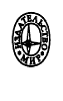
\includegraphics{2.png}

\large {МОСКВА «МИР» 1999}
\newpage

УДК 512+519.6

   ББК 22.14+22.19

\hspace{1.0cm} Н72
\\

\hspace{1.0cm} \textbf{Ноден П., Китте К.}

Н72 \hspace{0.5cm} \small {Алгебраическая алгоритмика (с упражнениями и решениями):} 

\hspace{1.0cm} \small {Пер. с франц. — М.: Мир, 1999. — 720 с., ил.}

\hspace{1.5cm} ISBN 5-03-003318-1

\hspace{1.5cm} \small {Книга известных французских математиков — это по существу эн-

\hspace{1.0cm} циклопедия алгоритмов алгебры и теории чисел от Евклида и до на-

\hspace{1.0cm} ших дней. В ней прослеживается общая идея — представить основные

\hspace{1.0cm} алгебраические структуры и концепции в виде объектов, поддающих-

\hspace{1.0cm} ся машинной обработке. Главными для авторов являются два вопроса:

\hspace{1.0cm} что значит вычислить математический объект и как его вычислить

\hspace{1.0cm} наиболее эффективно.

\hspace{1.5cm} Изложение отличается методическими достоинствами: тщательный 

\hspace{1.0cm} отбор материала, многочисленные замечания теоретического и исто-

\hspace{1.0cm} рического характера, большое число упражнений с решениями в конце

\hspace{1.0cm} каждой главы.

\hspace{1.5cm} Для математиков-прикладников, для всех изучающих и применяю-

\hspace{1.0cm} щих компьютерную алгебру и информатику как учебное и справочное 

\hspace{1.0cm} пособие.}

\hspace{4.0in} ББК 22.14+22.19
\\

\hspace{2.4in} 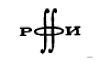
\includegraphics{1.png}
\\

\hspace{2.0cm} Издание осуществлено при поддержке Российского фонда 

\hspace{2.3cm}фундаментальных исследований по проекту 97-01-14001
\\\\

\hspace{2.5cm} Издание осуществлено в рамках программы помощи 

\hspace{2.9cm} издательскому делу «Пушкин» при поддержке 

\hspace{3.2cm} Министерства Иностранных Дел Франции

\hspace{4.0cm} и Посольства Франции в России
\\\\
 
\hspace{2.0cm} \textit {Редакция литературы по математическим наукам}
\\\\

ISBN 5-03-003318-1 (русск.) \hspace{2.1cm} © Masson, Paris, 1992 

 ISBN 2-225-82703-6 (франц.) \hspace{2.0cm} © перевод на русский язык,
 
\hspace{2.8in} «Мир», 1999
\newpage

\hspace{2.0cm} {\Large \textbf {Предисловие переводчика}

\hspace{2.6cm} {\Large \textbf {и редактора перевода}.
\\\\

    \normalsize {Со времени появления монографии Г. Биркгофа и Т. Барти «\textit {Современная прикладная алгебра}» (28 лет тому назад) сочетание прилагательных «\textit {прикладной}» и «\textit {абстрактный}» в применении к алгебре перестало шокировать или изумлять читателей. Прилагательное «\textit {современный}», разумеется, должно исчезнуть по мере разрастания теории и завоевания все новых территорий (переведенная недавно книга Р. Лидла и П. Пильца тому свидетельство). Более интересным является сопоставление компьютерной математики и алгебры, появившееся сравнительно недавно, а уж алгебраическая алгоритмика и вовсе должна вызвать ассоциацию с «\textit {маслом масляным}», ибо корни обоих понятий (алгебра и алгоритм), как известно, одни и те же. Тем не менее, несмотря на близкое родство, алгоритмика (читай, информатика) и алгебра длительное время развивались как бы обособленно, хотя слово «\textit {метод}» в учебниках по высшей алгебре вытеснялось постепенно словом «\textit {алгоритм}», а в информатику проникли модули и тензорные произведения. Вопросы сложности вычислений, явившиеся краеугольным камнем для информатики, позволили поставить весьма интересные чисто алгебраические задачи. Стало ясно, что в алгебре можно вычислять, даже если исходные вопросы касаются таких субстанций, как модуль, кольцо, группа. А раз можно вычислять, то нужно вычислять как можно быстрее, ибо уже студенту-первокурснику понятно, что «\textit грубая сила» машины не сможет выручить при решении некоторых совсем простых, на первый взгляд, задач.
    
   Многие алгоритмы алгебры, с которыми нам приходилось сталкиваться в жизни, становились известными из математического фольклора, другие изобретались самостоятельно (ибо посмотреть было негде). Потом появился изумительный Д. Кнут (Искусство программирования), пугающий своей фундаментальностью, куда все-таки приходилось заглядывать, невзирая на известные трудности. А что делать студенту? Книга «\textit {Алгебраическая алгоритмика}» явилась нам неожиданно во всем своем блеске благодаря знакомству с ее авторами, работавшими в Пуатье. Начав работать, мы оба поняли, что этой-то книги нам не хватало и как преподавателям, и как математикам-профессионалам.}
\newpage 
\setcounter{page}{6}% ВОТ ТУТ ЗАДАТЬ СТРАНИЦУ
С одной стороны, — это новый взгляд на вещи, казавшиеся устоявшимися. Например, что может быть проще алгоритма Евклида или возведения в степень? С другой, некоторая систематизация, азбука информатики (как мы мечтали 30 лет тому назад о каталоге полиномиальных алгоритмов!). Наконец, это философия программирования, изложенная на небольшом пространстве и без присущего сугубым профессионалам высокомерия.
В то же время книга читается (мы отмечаем это с некоторым ужасом) как художественная, беллетристическая литература. Чего стоит одно дерево Штерна — Броко из задачи 35 в главе II!

   Основной материал книги сопровождается огромным количеством упражнений (их около 300, но некоторые из упражнений содержат в себе от 3 до 5 задач), примеров, иллюстраций. Студента несомненно порадует то обстоятельство, что большинство упражнений приводится с решением (не сразу, а через несколько страниц). Пересечение с другими известными нам книгами по алгоритмике невелико.
Книга П. Нодена и К. Китте восполняет пробел, существовавший в литературе на русском языке (и по математике, и по информатике), и может быть использована для чтения специальных и основных курсов как для студентов-математиков, так и для информатиков. Кроме того, она, будучи использована в качестве дополнительного источника, окажется несомненно полезной при чтении курсов «Алгебра и теория чисел» и «Алгебра и геометрия».

   Следует отметить, что терминология, применяемая французскими математиками, не вполне совпадает с принятой в нашей литературе. Так, натуральный ряд начинается с нуля, а не с 1, как обычно принято у нас. Отсюда появление обозначения N*. Приведение матрицы к ступенчатому виду осуществляется по столбцам, а не по строкам, причем имени Гаусса авторы в этой связи не упоминают. Есть и другие мелкие детали, которые читатели, несомненно, заметят. Что ж, это заставляет читателя быть внимательным!

  Приятно отметить, что в подготовке к изданию перевода книги активное участие приняли наши ученики и студенты С.В. Монахов, С.М. Медведев (подготовившие оригинал-макет русского перевода), И.А. Сагиров, Л.В. Гудкова, А.В. Хлямков, А.Е. Скрипкин. Мы им выражаем нашу глубокую благодарность. Мы также признательны заведующему лабораторией теоретико-групповых методов профессору А.Л. Онищику за предоставление технических средств для верстки этой книги. Мы благодарны издательству MASSON, давшему согласие на передачу права на издание перевода книги издательству «Мир», и Посольству Франции в Москве включение русского издания книги
\newpage 
в программу «Пушкин», а также Российскому фонду фундаментальных исследований, поддержавшему проект перевода книги издательским грантом.

   В заключение мы хотим прямо сказать, что наш замысел вряд ли осуществился, если бы не помощь и активное сотрудничество наших французских друзей и коллег из университета Пуатье — авторов книги Патриса Нодена и Клода Китте. Они дали согласие на безвозмездное издание перевода их книги, любезно предоставили в наше распоряжение файлы с ее электронным вариантом и постоянно, на протяжении всего времени работы над переводом, поддерживали с нами связь, консультировали нас, полностью пересмотрели текст французского издания и внесли в него много исправлений и улучшений, которые учтены в русском издании.
   
   Только благодаря этому сотрудничеству наш совместный проект успешно завершен.
   
   Надеемся, что перевод этой примечательной книги будет интересен и полезен нашим читателям.


 \hspace{3.1in} \textit {Л.С. Казарин, В.А. Соколов,} 
   
\hspace{3.0in} \textit {Ярославль, 10 августа 1998 г.}
\newpage
\hspace{1.4cm} {\Large \textbf {Предисловие к русскому изданию}}
\newline\\
\hspace*{15pt}
\hspace*{15pt}
\\\\
Проект перевода Львом Казариным и Валерием Соколовым нашей кни-
ги «Алгебраическая алгоритмика», возникший более двух лет тому на-
зад, подошел к завершению. Мы особенно рады этому событию, ес-
ли учесть, что пройденный путь, вероятно, не был гладким. Основные очертания проект приобрел в результате нашего путешествия в Россию, которое мы предприняли весной 1996 года по приглашению Валерия Соколова от имени Ярославского государственного университета. Во время нашего пребывания в Ярославле Лев и Валерий оказали нам, как гостям университета, самый радушный прием. Лев сопровождал нас во всех поездках, которые Ярославский университет организовал для нас, чтобы мы открыли для себя маленький кусочек России — это то, что выходит за рамки профессиональной деятельности, но является, тем не менее, приятным (и необходимым) элементом любой поездки за границу. Благодаря Льву мы открыли ряд исторических уголков, входящих в «Золотое кольцо»; он опекал нас на первых шагах в нашей повседневной жизни иностранцев в России, что порой было очень непросто: вспомним автобус, который отвозил нас на вокзал в пятницу в 6 часов утра, когда все киоски были еще закрыты! «Автобус... А как насчет билетов?» А в Москве Аркадий Онищик, Сергей и Ирина Струнковы доказали нам на непостижимом для представителей Запада уровне, что российское гостеприимство вовсе не легенда. Обо всех этих встречах и людях мы сохраним самые волнующие воспоминания.

   Прервем здесь дифирамбы, хотя это вступление в действительности лишь в небольшой степени передает наше душевное состояние. Нелегкое, все-таки, это дело — сочинять предисловие к переводу книги, которую сами написали! Поговорим, однако, об идеях, которые мы хотели изложить в этой книге.

   В течение трех лет работы над ней (1989-91 гг.) нашей целью — амбициозной и одновременно наивной — было представить с одной конкретной точки зрения некоторые разделы алгебры, преподаваемые на старших курсах университета. В то время нам хотелось (и сейчас нам этого хочется более, чем когда-либо) изменений в изложении математики: не отказываясь от абстрактных понятий, использовать их так, чтобы гармонично сочетать теорию и практику.
\newpage
   Любой студент-математик знаком с основными понятиями, которые встречаются в арифметике: целые числа, сравнимость чисел по модулю п, многочлены и т.д. Но, чаще всего, эти объекты, по самой своей сути предназначенные для практики, определяются очень формально и абстрактно. Так ли уж необходимо вводить фактор-группу некоторой группы по отличной от нее подгруппе для изучения целых чисел, сравнимых по модулю п? Что усвоят наши студенты при таком подходе? Так ли уж неразумно опираться, когда это возможно, на практику? Ведь освоив вычисления по модулю целого числа (или по модулю многочлена), уже гораздо позже можно рассмотреть общий случай вычислений по модулю идеала, «более естественно» приводящий к понятию фактор-кольца. В самом деле, нет недостатка в конкретных проблемах, где может с успехом использоваться вычислительная практика: тест на простоту чисел Лукаса — Лемера, критерий Пепина, RSA-метод в криптографии, генератор случайных чисел и т.д. Мы рассматриваем все эти темы в нашей книге и убеждены, что они лучше подходят для обучения, чем «теорема о факторизации (переход к фактор-множеству) некоторого отображения».

   Что же изменилось с 1992 года, времени выхода нашей книги? В области математической алгоритмики на рынке появилось некоторое количество монографий, но это в основном узко специализированные книги научного характера, оказывающие весьма слабое влияние на преподавание математики. Что же касается информатики как таковой, то единственным плодом ее непрерывного бурного развития в данной области является увеличение числа систем формальных вычислений — часто настолько же мощных, насколько и непоследовательных, неприспособленных для научной работы из-за недостаточной строгости. Нынче можно осуществлять сложные вычисления в теории Галуа, в алгебраической геометрии, в теории чисел, в теории групп и т.д., но все это, как правило, недоступно для начинающего студента-математика. И против всех ожиданий, области, в которых системы формальных вычислений уже хорошо обкатаны — это, как ни странно, разделы курса алгебры — всегда излагаются в том же виде, в каком они были десятилетия назад. Использование этих прикладных программ осталось вне преподавания математики и касается, в основном, лишь научных исследований.

   Сообществу математиков, кажется, грозит опасность раскола на два чуждых друг другу мира: «теоретиков» и «алгоритмистов». Эта ситуация, на наш взгляд, была бы достойна сожаления. В то же время, во Франции — особенно в преподавании математики — нередко шли на отказ от догматических воззрений в пользу нового хорошего подхо-
\newpage
да к объяснению того или иного понятия. Преподавание (равно, как и научное исследование) может лишь обогатиться благодаря многообразию способов изложения материала: достаточно хотя бы раз в жизни прочитать студентам курс лекций по алгоритмике, чтобы убедиться в этом.

\hspace{3.8in} П. Ноден, К. Китте,
        
\hspace{3.3in} Пуатье, 2 февраля 1999 г.
\newpage
\hspace{1.4in} {\huge Предисловие}
\\\\\\\\
   Патрис Ноден и Клод Китте попросили меня написать предисловие к их книге, и я начну с благодарности им: быть вовлеченным в работу в приятной компании по случаю выхода в свет такого прекрасного произведения — это счастье.

   История математики очень увлекательна. Для сюжета, который нас занимает сегодня, существенны три персонажа. Евклид пишет свои «Начала» за три столетия до нашей эры, и с этой даты большинство историков ведут отсчет появления той математики, которую мы знаем сегодня, имеющей характер некой игры, заключающейся в том, чтобы делать интересные выводы из множества хорошо подобранных аксиом. Природа этих аксиом и соблюдаемые правила игры с самого начала не были достаточно ясны, и математика XIX века познала такое развитие, что вскоре основы здания были едва способны выдерживать всю конструкцию. Итогом этого было то, что называют кризисом оснований математики.

   Но тут появился Гильберт; он понял и талантливо объяснил, что математика может быть формализована. Гильберт описал работу математиков, как чисто формальную игру, манипулирующую множеством аксиом (комбинаторных объектов) с помощью доказательств (чисто комбинаторной техники) и приводящую к теоремам (также комбинаторным объектам). На самом деле так говорить — неправильно: Гильберт мог таким образом описать результаты, полученные его предшественниками, но никоим образом — с помощью какой процедуры они их открыли. Это главное различие для того сюжета, которым мы интересуемся. Гильберт знал это и вскоре поставил перед сообществом хорошие вопросы на эту тему: может ли аксиоматическая система быть полной, или, другими словами, всякое ли утверждение, имеющее смысл в этой системе, истинно или ложно? Кроме того, существует ли алгоритм, позволяющий определять, истинно или ложно то или иное утверждение (или же невыводимо в случае неполноты)?

   После Евклида и Гильберта третьим является Гёдель. Он доказал, что всякая аксиоматическая достаточно «интересная» теория обязательно будет неполной (или противоречивой). Этот явно негативный результат странным образом является одним из наиболее позитивных.
\newpage
Непосредственно вдохновленные доказательством Гёделя логики Чёрч и Тьюринг вскоре доказали (1936), независимо друг от друга и разными способами, что второй вопрос Гильберта также имеет отрицательный ответ: не может существовать алгоритм, даже чисто теоретический, грозящий математикам безработицей. Этот результат все еще отрицательный, но — терпение, и мы увидим, что на самом деле Чёрч и Тьюринг стоят у истоков фантастической — и позитивной — революции в математике. Ибо им пришлось очень тщательно обдумать, что же такое алгоритм. Первый из них изобрел для уточнения этого понятия A-исчисление, второй — свою знаменитую теоретическую машину. И это стало рождением целой новой ветви в математике, называемой алгоритмикой, и книга, которую я предваряю предисловием, частично относится к этой области. В этом ее новизна.

   Благодаря фон Нейману идеи Тьюринга вскоре привели к концепции и реализации того, что теперь называется компьютерами. Вначале в них видели лишь инструмент, предназначенный для того, чтобы использовать результаты труда математиков-теоретиков в различных приложениях. Этот взгляд, все еще распространенный, когда инфор- матик ниже по течению принимает эстафету от математика, является сегодня совершенно неверным. Больше уже не считают, что математические теории, представление о которых существенно изменилось, находятся в верховьях по отношению к положению алгоритмического инструмента, и ставить эту ветвь в подчинение другим так же наивно, как пытаться выяснить в алгебраической топологии, что главнее: топология по отношению к алгебре или наоборот.

   Математики все еще часто и довольно нелепо считают за честь получить результаты, не использующие новые алгоритмические средства. Это обычное явление, сопровождающее значительное и быстрое развитие в какой бы то ни было сфере жизни: подобное развитие порождает кризис, разрешающийся более или менее удачно. Когда возникла алгебраическая топология, многие строптивые топологи старательно отделяли топологические доказательства, не использующие алгебраическую топологию, считая их более хорошими, от других, незаконнорожденных. Но в конце концов алгебраическая топология утвердилась. В рамках алгебраической топологии в один прекрасный день появились спектральные последовательности', в это время доказательства, использующие такую технику, еще рассматривались как «грязные», и их, по-возможности, избегали. Мало-помалу, спектральные последовательности стали обычным делом. Совсем недавно новые исследования заново изучили вопрос, связанный со спектральными последовательностями, для того, чтобы сделать из них алгоритмический инструмент;
\newpage
я знал редактора одного прекрасного математического журнала, сердито требовавшего представить аргумент, «убеждающий», что новые результаты, полученные таким способом, были бы недоступны при использовании «других средств» (sic) и не иначе, без чего представленная статья на эту тему была бы, очевидно, отвергнута. S.O.S. — расизм!

   Книга Патриса Нодена и Клода Китте представляет классическую алгебру — ту, которая преподается на уровне второго цикла университета, но в свете новой алгоритмической идеологии. Для рассматриваемой темы алгебра подходит лучше всего: алгоритмика по самой своей природе комбинаторна, а среди всех основных математических дисциплин алгебра является, несомненно, «самой комбинаторной». Преподавать студентам алгебру таким способом — прекрасная идея с разных точек зрения. Очень полезно, что значительно усиливается конкретный характер теории, результатов, упражнений, отдельных тем; это облегчает понимание, требует хорошей точности, но и придает характер игры занятию, которое нередко воспринимается скучным и отталкивающим.

   Но есть еще более важное обстоятельство. Богатство, присущее математике, чаще всего требует, как, впрочем, и в любой сфере деятельности, использования сразу нескольких средств очень разной природы. Самые большие успехи в математике почти всегда могут быть описаны именно так. В другой области, теоретической физике, показательна работа Луи де Бройля, объясняющая, что правильно понять свойства материи можно, лишь рассматривая ее одновременно с волновой и корпускулярной точек зрения. Эйнштейн поступил аналогично в отношении массы и энергии, Гильберт — с геометрией и функциональным анализом и т.д. Так и с момента возникновения алгоритмики всякая попытка пересмотреть тот или иной раздел математики с точки зрения алгоритмики может быть встречена с интересом и надеждой.

   Так устанавливаются взаимные связи, природа которых богата и разнообразна. В некоторых случаях алгоритмика оказывается на службе у обычной математики, являясь тогда инструментом прикладной математики. Часто использование средств алгоритмики порождает новые области математических исследований. Проблемы сложности вычислений, составляющие значительную часть данного труда, — это как раз тот самый случай. Замечу, кстати, что именно к этой области принадлежит самая важная открытая проблема современной математики — сравнение сложностей Р и NP; если, основываясь на сравнительном подобии, распространить математику на все науки, то проблемы Римана, Пуанкаре, «обратная теорема Галуа» окажутся где-то недалеко от химии, тогда как проблема $P \neq N P$ не выйдет за пределы математики.
\newpage
   Иной раз алгоритмические проблемы порождают новый сюжет, который может быть затем полностью отделен от источника своего происхождения и превратиться в раздел «чистой» математики. Хоть исторически это и не вполне корректно, но таким образом можно представлять студентам гармонический анализ. Одна из глав этой книги посвящена дискретному преобразованию Фурье. Даже если бы Фурье не существовал и даже если бы никто с тех пор не мог его заменить, все равно алгоритмика умножения многочленов обязывает обнаружить так называемый анализ Фурье, его интерес, его богатство и его эффективность. А потом уже нетрудно, переходя к пределу, получить ряды Фурье и преобразование Фурье, исходя из дискретного преобразования Фурье; наиболее просто это сделать, используя нестандартный анализ — но берегись инквизиторов: сочетая две ереси в одном курсе, рискуешь сломать себе шею, если не быть осторожным или попросту скромным!

  Другой интересный случай, представляющий, несомненно, очень богатый сюжет: для некоторой ранее существовавшей математической теории ее пересмотр может привести к таким точкам зрения, которые требуют иных методов, имеющих свой собственный интерес, не уменьшая, однако, тем самым, интерес к исходным теоретическим методам. Хорошим примером такого сорта является матричное исчисление. Классическая теория определителей, на базе знакопеременных полилинейных форм, непосредственно не используется при вычислении определителей. На самом деле ситуация даже еще лучше. Наши самые далекие предшественники, несомненно, были знакомы с сущностью так называемого метода Гаусса решения систем линейных уравнений. Однажды появились теоретики и вообразили, что лучше это делать с помощью определителей. Потом алгоритмисты снова поправили стрелки часов: для машины метод Гаусса намного лучше, чем метод Крамера, что, однако, вовсе не лишает интереса к этому методу, который с успехом используется для теоретического анализа первого. Этот и другие связанные с ним вопросы изящно изложены в данной книге; содержащаяся в ней обширная библиография и комментарии позволят прилежным читателям быстро добраться до современных проблем, о богатстве которых они вначале и не подозревали.

   Информатики сразу распознают одного из духовных наставников авторов: Дона Кнута. Отметим лишь составление макета книги, полностью реализованное самими авторами (без Postscript’а!) с помощью TEX'a. Мне не известна официальная градация в сообществе TEX пер-тов, но, несомненно, Патрис Ноден и Клод Китте в его первом эшелоне.
\newpage
   Вошло в поговорку безграничное богатство анализа всех аспектов проблемы в книгах Кнута; то же самое мы обнаруживаем здесь. Для читателя, раполагающего достаточным временем, эта книга — неисчерпаемый кладезь возможностей рассматривать отдельную тему с множества точек зрения. Когда, говоря о программе, авторы решаются перейти к следующей теме, они не забывают заранее указать полезную библиографию; часто это даже библиография в квадрате, содержащая цитируемые тексты, которые, в свою очередь, также содержат обширную библиографию — изящный пример использования подпрограмм. Как и у Кнута, в этой книге имеется обширный набор упражнений разного уровня — от простых примеров, предназначенных проверить понимание того или иного понятия, до самых сложных задач, приближающихся к темам научных исследований. И, как и у Кнута, решения упражнений также включены в книгу!

  Для изучения алгоритмов требовалась техническая поддержка в виде языковых средств информатики. Авторы выбрали язык Ада — безусловно, один из лучших на сегодня языков. И пусть потенциальные пользователи не волнуются по поводу выбора языка, все еще не слишком распространенного во французских университетах: перевод Ада- программ в их любимый язык является несложным техническим упражнением; при этом строгость документации программ просто поразительна и может служить примером, так что на этот счет нет никаких опасений. Такой перевод, требующий ясно отличать алгоритмическую часть от реализации, очень поучителен. Кроме того, авторы зачастую предварительно дают описание алгоритмов в чистом виде в соответствии с аксиоматикой Хоара.

   Это превосходная книга, которую я ставлю в моей библиотеке на полку со «священными» книгами, где находятся уже два «евангелия» — алгоритмика по Вирту и алгоритмика по Кнуту. Теперь я обладаю третьим «евангелием»; кто же напишет четвертое? Но ведь эта книга потребовала коллективной работы двух авторов — еще одно примечательное свойство, так что может быть моя коллекция «евангелий» уже полна? Нет: это противоречило бы Гёделю, но это уже совсем другая история.
   
\hspace{3.6in} Франсис Сержераер,

\hspace{3.1in} Мейлан, 27 сентября 1991 г.
\newpage
\hspace{1.5in} {\huge От авторов}
\\\\\\\\
   Вот и наступил момент, когда, закончив книгу, автор начинает свое введение и ищет подходящие формулировки, которые убедили бы читателя, что все дальнейшее было спланировано, обосновано... с самого начала. Мы не будем отступать от этого правила. Однако, скажем откровенно, наша точка зрения изменялась многократно с того момента, когда мы принялись за этот труд.

   Вопрос «Возможно ли вычислять математические объекты?» является лейтмотивом этой работы; как можно убедиться, эта книга не дает окончательного ответа, но, надеемся, показывает, что этот вопрос не лишен интереса. В особенности в той области, которую затрагиваем здесь, а именно, в алгебре, мы убеждены, эффективное вычисление объектов — вручную или с помощью компьютера — проливает свет на используемые понятия. Но, начиная с таких элементарных понятий, как кольцо целых чисел по модулю п, и до более абстрактных структур, как модули в основных кольцах, что же все-таки можно вычислять и как? В начале работы мы были совсем уже готовы уступить намерению рассматривать алгебру без каких бы то ни было формальных средств, а только в чисто вычислительном аспекте; но изучение преобразования Фурье — и, в особенности, работы Ш. Винограда — убедительно подтолкнули нас к тому, чтобы избежать этого соблазна. В результате проект, сознательно ограниченный вначале, стал более полновесным и содержательным; мы даже позволили себе сочинить полную главу, посвященную дискретному преобразованию Фурье, с включением в нее билинейных форм и тензорного произведения; добавили раздел, излагающий классический подход к факторизуемости колец многочленов...

   Однако мы не отказались от главной идеи, которая составляет основу этой книги: можно вполне конкретно представить понятия элементарной алгебры, т.е., опираясь на учебные примеры и приводя, по мере возможности, конструктивные доказательства.
   
\hspace{0.8in} \small  \textit {Возьмем для примера теорему Цермело, согласно которой}

\hspace{0.6in} \small  \textit {пространство можно преобразовать во вполне упорядоченное}

\hspace{0.6in} \small  \textit {множество; приверженца Кантора будут очарованы строгостью}

\hspace{0.6in} \small  \textit {доказательства — действительной и кажущейся; прагматики}

\hspace{0.6in} \small  \textit {им возразят: Вы утверждаете, что можете преобразовать про-}
\newpage

\hspace{0.6in} \small \textit {странство во вполне упорядоченное множество; ну что ж, пре-}

\hspace{0.6in} \small  \textit {образуйте его! — Это слишком долго. — Тогда покажите нам }

\hspace{0.6in} \small  \textit {по крайней мере, кого-то, кто нашел бы достаточно времени и }

\hspace{0.6in} \small  \textit {терпения и кто смог бы выполнить это преобразование. — Нет, }

\hspace{0.6in} \small  \textit {мы это не можем, потому что число необходимых для этого опе-}

\hspace{0.6in} \small  \textit {раций бесконечно, оно даже превосходит Ко- —А можете ли вы }

\hspace{0.6in} \small  \textit {показать, как можно было бы выразить конечным числом слов }

\hspace{0.6in} \small  \textit {то правило, которое позволило бы упорядочить пространство?} 

\hspace{0.6in} \small  \textit {— Нет — и прагматики делают вывод, что эта теорема или }

\hspace{0.6in} \small  \textit {лишена смысла, или неверна, или же, по меньшей мере, недока-}

\hspace{0.6in} \small  \textit {зуема.}


\hspace{1.8in} \small  \textit {Анри Пуанкаре, Последние мысли (1913 [161])}
\\\\

   Это идет вразрез с общепринятой практикой, которая заключается в преподавании математики на абстрактном уровне, без опоры на эксперимент, как в других научных дисциплинах. Скольких хлопот избегают при этом! Гораздо легче, например, доказать существование для любого простого числа р примитивного по модулю р многочлена, нежели построить процедуру, порождающую за 5 шагов в периоде длины 32 примитивный по модулю 2 многочлен $X^5 + X^2 + 1$.

   Эта книга рискует удивить читателя; в ней иногда объясняются очень простые вещи, а иногда быстро проходят через более сложные понятия. Часто используются понятия группы, модуля, кольца, тела и т.п., но ни одно из этих понятий не определяется; существуют прекрасные книги по алгебре, содержащие эти определения, и нам хотелось не перефразировать их, а скорее попытаться взглянуть на эти структуры с точки зрения эффективности. Всякий раз, когда нам это представлялось возможным, мы стремились заменить традиционную манеру изложения темы и показать многосторонние связи между различными понятиями (например, различные типы колец в теории делимости, сходство между конечными абелевыми группами и редукцией эндоморфизмов и т.д.). Выбор рассматриваемых тем не бесспорен. Мы мало внимания уделяли многочленам, которые, однако, являются фундаментальными объектами в алгебре; в то же время сравнительно много внимания посвящено дихотомическому алгоритму возведения в степень и алгоритму Евклида. Цель, которую мы перед собой ставили, — изучить небольшое количество методов, относящихся к области, называемой ныне алгебраической алгоритмикой, стараясь связать их между собой и с классическими понятиями алгебры. Этот вывод привел нас к сознательному отказу от рассмотрения таких сюжетов как, например,
\newpage
теория Галуа или теория групп, которые очевидным образом допускают алгоритмический подход. Таким образом, мы стремились предоставить необходимые средства для углубленного изучения этой дисциплины, оседлавшей математику и информатику. В действительности, существо описанных в данном курсе методов сконцентрировано в четырех основных алгоритмах: дихотомический алгоритм возведения в степень, алгоритм Евклида, китайская теорема об остатках и быстрое преобразование Фурье; они образуют основу для любой системы формальных вычислений. Тем не менее, в упражнениях содержатся введения в различные темы: от пошаговой трассировки до символа Якоби, включая р-адические числа, непрерывные дроби, многоразрядную арифметику...

   Введение в предмет составляют основы информатики, необходимые для того, чтобы недвусмысленно рассуждать об алгоритмах, об их обоснованиях, о программах. Объекты информатики, определяемые здесь, очень разнообразны: от начал программирования очень быстро переходим к таким понятиям, как модулярность, шифрование информации, порождаемость..., затрагивая весьма тонкую технику программирования на языке Ада. И вот великое слово произнесено! На самом деле большинство реализаций алгоритмов, которые мы даем, написано на языке Ада. Многие удивлялись, что не был выбран Лисп (и мы готовы спорить), Паскаль или Си (в данном случае спор с нами бесполезен). Ада обладает той строгостью, которая, как нам кажется, вполне гармонирует с математической строгостью; мы также широко пользовались богатством систем контроля в языке Ада как для программирования, так и для описания алгоритмов.
\\\\

\hspace{1.0in} \small  \textit {Программисту на языке Лисп известно значение всего, но он} 
   
\hspace{0.8in} \small  \textit {никогда не знает, сколько это стоит.}
\\\\

\hspace{1.5in} \small  \textit {Алан Дж. Перлис, Программистские эпиграммы (1978)}
\\\\

   Пусть сторонников языка Лисп не смущает эта цитата. Мы далеки от того, чтобы быть невосприимчивыми к этому языку. И если мы по достоинству ценим определенные аспекты языка Ада, то мы всегда сожалели о хронической нехватке некоторых базовых средств в этом языке (арифметика высокой точности — лишь один тому пример).

   Выбор материала по информатике для включения в эту книгу был труден: она адресована в первую очередь не информатикам, а математикам, чьи познания в информатике не всегда достаточно основательны. Тем не менее, в этой книге мы не предполагаем, что читателю
\newpage

%%\documentclass{mai_book}
%\defaultfontfeatures{Mapping=tex-text}
%\setmainfont{DejaVuSerif}
%\setdefaultlanguage{russian}
%\usepackage{amsmath}
%\usepackage{floatflt}
%\usepackage{wrapfig,lipsum,booktabs}
%\begin{document}

	\noindent совершенно чужд этот предмет; однако, возможно, он будет удивлен не­
	обычным  подходом  в  математике.  В  информатике не редкость,  когда 
	формулировка проблемы  бывает такой  же  длинной, как  и  ее  решение.

	В книге приведены несколько полных программ; они предназначены 
	не для  «производственных целей»,  а для построения  поучительных при­
	меров. И хотя мы не включили все программы, реализующие описанные 
	методы,  — книга бы  просто  лопнула...  такж е,  как  и  наш  издатель  — 
	тем  не  менее,  все  описанные  методы  реализованы  или  на  языке  Ада, 
	когда  имевшиеся  в  нашем  расположении  средства  это  позволяли,  или 
	в среде системы формализованных вычислений  Scratch pad. Эта систе­
	ма была выбрана не за cвои мнимые достоинства или за как будто бы 
	богатое программное обеспечение, а исключительно потому, что она 
	была нам доступна и позволяла умножать числа с 100 знаками. И ес­
	ли слабость и неадекватные реакции ее компилятора довольно быстро 
	обескуражили одного из авторов, то другой еще продолжает борьбу.
	
	Мы должны особо упомянуть наш основной источник вдохновения 
	—  монументальный труд Дональда Кнута «Искусство программиро­вания».
	  Часто нам случалось самостоятельно или в процессе чтения 
	открыть
  	некий  новый  алгоритм; так  вот,  мы  можем  утверждать,  что 
	более,  чем  в  70\%  случаев,  оказывалось,  что  этот   алгоритм  уже  был 
	описан  в  его  книге  и  чаще  всего  гораздо  лучше, чем там , где мы  его 
	нашли.  Мы  не  можем  упоминать  Кнута  на  каждой  странице,  где  явно 
	присутствует  его  вклад,  ибо его  имя  появлялось бы  сотни  раз.  Мы это 
	делаем здесь.
	
	Помимо этой  серии  книг,  еще  не  оконченной  в  настоящий  момент, 
	Кнут также  реализовал — чтобы  иметь  возможность  точного написа­
	ния  своих  книг  —  компилятор  текстов 
	поистине  феноменальной 
	мощности.  Эта  книга  смогла  быть  написана  ее  авторами-любителями 
	благодаря Кнуту  и  многочисленным  бессонным  ночам  в  попытках  по­
	нять внутренние механизмы \TeX 'a.  Без  \TeX 'a мы никогда бы не смогли 
	реализовать  нашу  книгу  в  данном  виде.  И  вот  теперь  мы  можем,  на 
	манер  Кнута,  сказать: 
	\textit{If this book has any merit,  the credit should go to
	Knuth...  On the other hand, if this book has deficiencies,  the biaim should
	be directed to us ...} \footnote{Если эта книга имеет достоинства, это заслуга Кнута... С другой стороны,
	если в этой книге есть недостатки, то упрек должен быть адресован нам,..}

	Даниель  Лазар  и  Франсис  Сержераер  первыми  связали математи­
	ку и информатику в процессе преподавания в Пуатье. Мы им обязаны 
	определенной концепцией преподавания этих дисциплин и считаем сво­
	им долгом поблагодарить их здесь.	
	
	Эта книга не является творением двух отдельных личностей; мы 
	пользовались советами  наших  многочисленных  коллег.  Мы  особенно 
	благодарны Пьеру Берна, Жан-Мари Гурсо, Жан-Луи Паско, Мустафе 
	Раису, Ги Рено и Жаку Валетту; мы обязаны не только идеями упраж­
	нений, доказательств, но также и другой точкой зрения на ряд мето­
	дов,  излагаемых  в этой  книге.  Мы  благодарим такж е сотрудников фа­
	культета математики  и  информатики университета Пуатье.  В течение 
	всех тех лет,  когда шла работа над  книгой, мы ощущали их поддержку 
	и  симпатию.  Успешное  продвижение  проекта  было значительно облег­
	чено  предоставлением  места  работы  в  лаборатории  первому  автору и 
	\textit{творческого} отпуска —  второму.
	
	Мы  не  забываем  студентов  специального  курса  «Информатика для 
	математиков»,  которые  на протяжении  многих лет  вносили  различные 
	поправки  и  предлагали  идеи.
	
	Мы  не  можем  на  этом закончить,  чтобы  не  подмигнуть Жаку Боровчику,
	без  которого  не  осмелились  бы  написать  эту  книгу,  а также 
	Жан-Пьеру  Раду,  виновному  за   выбор  языка  Ада,  Ливью  Соломону, 
	дававшему  нам  советы  по  разным  случаям,  и  Бернару  Гарро,  который 
	неотлучно  был  с  нами  в течение  всей  этой  работы.
	
	Что же  касается  якобы очень  взаимообогащающей  работы  вдвоем, 
	то это не всегда было очевидным, и проблемы не всегда были столь 
	же просты, как эта: << — Почему ты  вставляешь цитаты  по-английски? >>
	Некоторые  читатели  не  поймут.  — Я  предпочитаю  оригинальную  вер­
	сию, которая содержит в себе порой непереводимый  юмор. — Ну, а как 
	насчет цитат на немецком?  —  Ну это совсем другое дело. Я не знаю 
	немецкого».
	
	Эта  книга посвящается всем нашим друзьям, которые нас поддер­
	живали и мирились с нашим переменчивым настроением в течение этих 
	трех сумасшедших лет.
	\chapter{Алгоритмика и \newline программирование на \newline языке Ада}
	\noindent В этой главе — вероятно самой «информатической» в нашей книге —
	мы введем некоторые алгоритмические понятия и опишем несколько
	получисленных алгоритмов, необходимых для реализации алгебраиче­
	ских методов.
	
	Точное определение алгоритмических границ, в которых будут из­
	ложены методы вычисления, станет предметом особого внимания. Цель
	нашего труда не ознакомить с основами алгоритмики — предполага­
	ется, что читатель не новичок в данной области, — а определить без­
	укоризненным способом семантику построений, используемых в алгоритмах\footnote{Что совсем не умаляет ни корректность (верность) программ, которые можно
	будет потом получить, ни соответствие компилятора его спецификациям. Эти усло­
	вия,  однако, необходимы для  истинности математической теоремы,  доказанной с
	помощью компьютера.}.
	
	После изложения общих направлений мы приступим к исследова­
	нию первого фундаментального алгоритма этой книги: дихотомиче­
	ского алгоритма возведения в степень. Для этого будут использоваться
	два метода построения алгоритмов. Один очень близок к математиче­
	ским рассуждениям, другой — чисто алгоритмический. При этом у нас
	появится возможность открыть первый рекурсивный алгоритм, пред­
	ставленный в данной работе.
	
	Начав с первого примера алгоритма, мы перейдем к изучению на­
	чальных понятий программирования на языке Ада. И здесь тоже речь
	пойдет не об изложении полного курса языка Ада, а только о пред-
	
	\pagebreak
	\noindent ставлении нескольких ключевых понятий, необходимых для понимания
	приведенных программ.
	
	Вообще говоря, все понятия будут представлены (по мере надоб­
	ности) на примерах, во избежание их формального описания (по по­
	следнему вопросу лучше обратиться к справочному изданию: Reference
	manual for the Ada programming language\footnote{См. книгу [186]. — Прим, перев.} ).
	
	И наконец, завершит эту главу разработка совершенно неэффек­
	тивного метода вычисления определителей целочисленных матриц. Об­
	суждаемый метод, основанный на математическом определении детер­
	минанта, позволяет наилучшим образом использовать все возможности
	современных компьютеров и получить идеальное приближение к беско­
	нечности на машине! Кроме того, обсуждение ситуации позволит нам
	несколько пополнить представление о программировании на языке Ада.
	
	\section{Введение в алгоритмику}
	\noindent Прежде чем приступить к описанию любого алгоритма, нужно ого­
	ворить общепринятые соглашения, используемые в работе. В инфор­
	матике чаще, чем в любой другой дисциплине, встречается взаимное
	непонимание между пользователем и разработчиком новых программ.
	Поэтому так важно сформулировать аксиоматику, позволяющую связ­
	но рассуждать об алгоритмах.
	
	Множество аксиом, которое мы собираемся сейчас описать, извест­
	но как \textit{аксиоматика Хоара} [86], в честь исследователя, который первым
	формализовал семантику структур и действий последовательной алго
	ритмики.
	
	\subsection{Терминология и обозначения}
	
	\noindent \textbf{Алгоритм} — это последовательность более или менее элементарных
	действий, которая позволяет пошагово решить поставленную задачу за
	конечное время. Можно формально по индукции определить, что та­
	кое алгоритм, нижеследующим образом. Цель этого введения в алго­
	ритмику — изучение и представление всех терминов, фигурирующих в
	предыдущем определении (стиль определения, который в информатике
	называется \textbf{грамматикой}).
	
	Можно описать алгоритм в терминах состояний системы: состояние\linebreak
	системы\: до\: применения\: алгоритма,\: состояние\: той\: же\: системы\: после
	\pagebreak
	
\noindent применения алгоритма. Эти два состояния образуют то, что называет­ся спецификацией задачи.\: Таким\: же\: образом\: можно,\: описывая\: поэтапно

\begin{wraptable}{i}{0.55\textwidth}
\begin{tabular}{|l|}
\hline
\textit{\textbf{\begin{tabular}[c]{@{}l@{}}
	\text{$                  $} \\
	$\bullet$ Алгоритм — это действие \\
 	$\bullet$ Действие — это:\\
 		--- элементарное действие\\
 		--- последовательность действий\\
 		--- альтернатива \\
 		--- итерация\\
 	 $\bullet$ Элементарное действие — это:\\
 		--- пустое действие\\
 		---присваивание  —  ...\end{tabular}}} \\
	\text{$                  $} \\
\hline
\end{tabular}
\end{wraptable}
\noindent последовательные состоя­ния\linebreak
(между действиями) рассма-­\linebreak
триваемой системы, проводить обоснование алгоритма.Систе­ма доказательства по Флой­ду[71] --- это способ формализа­ции 
данного процесса. Но эта ак­сио-
\noindent матика не просто метод дока­зательства: в случае ее обобще­ния она может претендовать на роль хорошей методологии програмирования.
\newline

Состояния данной системы выражаются в виде утверждений, т.е.
логических формул. Рабочие гипотезы алгоритма называются
предусловиями или данны ми алгоритма. Заключения называются
постусловиями или результатам и. Вот, например, способ
формального описания алгоритма:
\begin{center}
[предусловия] Алгоритм [постусловия]
\end{center}
И это то, что можно назвать \textbf{спецификацией} алгоритма. Используя 
данную форму выражений, можно описать аксиомы Хоара в следующем 
виде:
\newline
\noindent $\vartriangleright$ \textit{Посылки} : предварительные условия к применению аксиомы. Эти 
условия  выражаются,  в  основном,  в  терминах  преобразований  утвер­
ждений посредством некоторых действий.
\newline
$\vartriangleright$ \textit{Заключение} : результат построения, которым описывают аксиому.
\subsection{Присваивание}
\noindent Это элементарное  действие,  наиболее опасное  и  наиболее трудное  для 
понимания  в  последовательных  алгоритмах.  Его  семантика  чрезвы­
чайно  проста:  переменной  (иногда очень  сложной)  придают  значение 
какого-либо выражения.  Действие  присваивания  представляется  в  ал­
горитмах, как правило, двумя способами: обычно с помощью стрелки, 
направленной  влево,  а  иногда  последовательностью  знаков  «:=»,  как, 
например, в языках программирования.
\newline
\textbf{(1) Аксиома} (присваивания).
\newline
$\vartriangleright$ \textit{Посылки: х является переменной,  e  —  выражением}
\newline

\noindent $\vartriangleright$ \textit{Заключение: [] х $\leftarrow$ е [x = значению е]}
\pagebreak

Интерпретация  этой  аксиомы  следующая:  нет  никакого  предусло­вия,  кроме  природы  его  операндов,  для  использования  присваивания. 
Каково  бы  ни  было состояние  системы,  сведенной  к  переменной х,  по­сле выполнения присваивания х будет иметь то же самое значение,  что и е.

Если задействовано несколько переменных,  то иногда форму посту-
­словия  присваивания  модифицируют.  Возьмем,  например,  систему,  
со­сто-
ящую  из  двух  переменных х  и у,  предположим  к  тому  же,  что у
имеет значение  е.  Выполним предыдущее  присваивание. В предусловие 
можно включить  переменную у,  хотя она не  входит в присваивание.  В 
результате имеем: $[y = e]$. Довольно часто вместо того, чтобы писать 
постусловие  в  виде  $[y = e \text{ и } x = e]$,  запись  сокращают  до  $[x = y]$, 
 что, разумеется,  приводит  к  исчезновению  некоторой  начальной  информа­ции.
 
Все  это  может  показаться  тривиальным,  и  обычно  совершаемая 
ошибка  состоит  в  смешении  присваивания с  частной  формой  записи 
уравнений (в математическом смысле)  или подстановкой. Простой при­мер,  иллюстрирующий  трудность  проблемы,  относится  к  системе  из 
двух переменных  и  предыдущему  условию
\begin{equation*}
\textit{$[\Re(x,n)] n \leftarrow n + 1 [\Re(x,n - 1)]$}
	\end{equation*}
где $\Re$ - отношение,  связывающее соответствующие значения двух его 
аргументов.
\subsection{Последовательность}
\noindent Это  алгоритмическая конструкция,  заключающаяся  в соединении дей­ст-
вий  в цепочку.  Ее часто представляют с помощью знака «;», который 
служит связкой  между  последовательными  действиями.  Эта конструк­ция
 самая простая среди тех, которые встречаются в последовательных 
алгоритмах.

Если А и В — действия,  то обозначим  через  «А ; В» действие, 
со­стоящее из последовательности действий А и В в данном порядке. Эта 
горизонтальная запись обладает некоторыми неудобствами, так что 
очень часто ту же последовательность действий записывают, распола­гая
вертикально на одной прямой действия одной и той же последова­тельности
(и аннулируя, в случае необходимости, знак «;»).
\newline
\textbf{(2) Аксиома} (последовательности).
\newline

\noindent $\vartriangleright$ \textit{Посылки: А и В --- действия, P, Q и R} --- утверждения
\begin{center}
\textit{$[ P ]\textit{ }A\textit{ }[ Q ]  \text{ и } [Q]\textit{ }B\textit{ }[ R ]$}
\end{center}
\pagebreak
$\vartriangleright$ \textit{Заключение:  [Р] А; В [R]}
\newline

Эта  аксиома  просто  выражает  тот  факт,  что  в  последовательно­сти 
двух действий  предусловие  второго является  постусловием  перво­го.
Иными словами, два действия одной и той же последовательности, 
следующие  одно за другим,  действуют  совместно.  Второе  использует 
результаты первого.

Вот очень простой пример, позволяющий конкретизировать преды-\linebreak
дущее  высказывание.  Рассмотрим систему,  образованную тремя цело­-\linebreak
численными переменными: \textit{C, x} и \textit{n}, и предположим, что эти перемен­-\linebreak
ные удовлетворяют следующему свойству (которое будет предусловием \linebreak
этой последовательности):\textit{$[C\times x^{n} = x_{0}^{n_{0}}]$}, где \textit{$x_{0}$} и \textit{$n_{0}$} --- две це-\linebreak
лочисленные константы. Последовательность действий, которую при­-

\begin{wraptable}{r}{0.18\textwidth}
\vspace{-20pt}
\begin{tabular}{|l|}
\hline
\textit{\begin{tabular}[c]{@{}l@{}}\textit{C $\leftarrow$ C $\times$ x}\\
\textit{n $\leftarrow$ n - 1}\end{tabular}} \\ 
\hline
\end{tabular}
\vspace{-10pt}
\end{wraptable}
\noindent меняют к этой системе, представлена справа. Пре­-\linebreak
образуем сначала исходное утверждение, используя тот 
факт, что 
\noindent n > 0 и \textit{$[C\times x^{n-1} \times x = x_{0}^{n_{0}} \text{ и } n > 0 $]}, и применим
первое  действие  последовательности, придав С значение, полученное 
при умножении его начального значения на х.Это выражается в 
пре­дыдущем утверждении слиянием двух первых термов левого члена 
ра­венства:\textit{$[C\times x^{n-1} = x_{0} \text{ и } n > 0]$}. Потом, рассматривая это новое 
утвер­ждение как  предусловие,  применим  второе действие, которое состоит 
в уменьшении значения \textit{n} на единицу.

Таким образом, получаем постусловие  рассматриваемой последова­тельности
 действий \textit{$[C\times x^{n} = x_{0}^{n_{0}} \textit{ и } n \geqslant 0]$}. Это последнее преобразова­
ние является примером типичного случая, упомянутого в конце преды­дущего раздела.

\subsection{Альтернатива}
\noindent Альтернатива — это структура управления,  соответствующая приня­тию решения в алгоритме. Ее часто выражают в виде «если ...  то  ...». 
Во всех алгоритмах, представленных в книге, структуры управления и 
примитивные конструкции будут записаны на английском языке, в 
ви­де схем, близких к языку Ада.  Этот прием имеет два важных 
преиму­щества: во-первых, алгоритмы пишутся на алгоритмическом диалекте, 
приближенном к языку  программирования; и потом,  выбранный язык 
Ада чрезвычайно точен  (небольшой эвфемизм!)  и достаточно понятен 
для записи алгоритмов.

Нет необходимости объяснять действие структуры  управления.  Ее 
семантика тождественна семантике, используемой в разговорном языке.
\newline
\pagebreak

\noindent \textbf{(3) Аксиома} (Альтернатива).
\newline
$\vartriangleright$ \textit{Посылки: А и В --- действия; С --- предикат, P и Q --- условия.}
\begin{center}
\textit{[ P и С] A [ Q ]  и [Р и (не С)] B [ Q ]}
\end{center}

\noindent $\vartriangleright$ \textit{Заключение:  \textbf{if} \textit{C} \textbf{then} \textit{A} \textbf{else} \textit{B} \textbf{end if}} [ Q ]
\newline

\noindent Прежде всего эта аксиома выражает тот факт, что какова бы ни 
была  ветвь  используемого  теста\footnote{ Ветвью теста называют каждую часть альтернативной структуры: часть «то*
или часть «в  противном случае»}, получаем  один  и  тот  же  результат 
(благодаря разделению действий А и В).

Если продолжить анализ, то из этой аксиомы можно извлечь некото­рую
 философию  (или  методологию)  программирования.  В  самом деле, 
можно субъективно объяснить такой подход и сделать вывод, что хоро­шая
альтернативная структура (т.е. альтернатива, простая для понима­ния
доказательства)  — это конструкция, в которой действия,  предста­вленные
в каждом  из  ответвлений, очень  похожи.  Не редко,  например, 
можно  встретить  в  программах  начинающих,  а  также  в  работах лю­
дей  более  опытных  (что  красноречиво  свидетельствует  об  их опыте!) 
альтернативные структуры, в которых в зависимости от того, является 
истинным или ложным предикат, совершается вычисление с внутренни­ми
 переменными  или выполняется действие  с промежуточным резуль­татом 
 (обычно на экран выводится сообщение). Конечно, эти програм­
мы  могут  быть  правильными  и,  следовательно,  вполне  доказуемыми, 
но  ценой  каких  искажений  в  изложении  алгоритма  и  в  формулиров­ках
  утверждений!  Не  говоря  уже  о  том,  какой  будет через  несколько 
месяцев степень понятности программы этого программиста! Зато хо­роший
 алгоритм не содержит особенностей, сопровождается простыми 
и ясными утверждениями и потребует намного меньше затрат во время 
его возможной доработки.

В качестве примера рассмотрим следующую альтернативу, предста­вля-
ющую небольшую  часть  дихотомического  алгоритма возведения  в 
степень,  который мы рассмотрим в дальнейшем.  Возьмем снова систе­му, состоящую из трех целочисленных переменных С, х и n, удовлетво­ряющую условию:
\begin{equation*}
\textit{$[C\cdot x^{n} = x_{0}^{n_{0}} $ и $ n > 0]$}    \eqno(1)             
\end{equation*}
Исходя  из  этой  системы  переменных,  применим  нижеследующий  эле­
ментарный   алгоритм,   который   в  основном  записывают  в   виде:
\newline
$\blacktriangleright$ \textbf{if} \text{ \textit{n нечетно }} \textbf{ then } \textit{$C$} := \textit{$C$} $\ast$ \textit{$x$}; \textbf{end if};$\blacktriangleleft$ Ключевое слово \textbf{null}
\pagebreak

\begin{wraptable}{i}{0.28\textwidth}
\begin{tabular}{|l|}
\hline
\textit{\begin{tabular}[c]{@{}l@{}}
	\textbf{if} (\textit{n - нечетно})\\
	\text{	 С = С} $\times$ x\\
	\textbf{else} null\end{tabular}} \\
 \hline
\end{tabular}
\vspace{-10pt}
\end{wraptable}
\noindent является примитивом алгоритмического языка, 
выражающим пустое действие (для структура­
листов это действие является нейтральным эле­ментом 
ассоциативной операции последователь­ной композиции). Семантика пустого действия 
та­кова (для любого утверждения Р):  [Р]  \textbf{null} [Р].

Итак, необходимо отдельно исследовать влияние действий каждой 
из двух ветвей теста на исходное утверждение, учитывая значение 
пре­диката «n нечетно». Сначала можно записать: \textit{n = 2q + г}, деление с
остатком \textit{n} на 2; \textit{q} --- это неполное частное, а \textit{r} --- остаток. Когда \textit{n}
и \textit{p} --- целые числа удобно обозначить через n/р неполное частное  от 
деления с остатком \textit{n} на \textit{p} и через \textit{n mod p} --- остаток при этом делении; 
учитывая вышесказанное,  получаем: \textit{n = 2(n/2) + т mod 2}. Кроме того, 
значение \textit{n mod 2} выражает четность \textit{n}. Исходное  утверждение  может 
быть преобразовано в
\begin{equation*}
[C\times x^{2(n/2)+n\text{ }mod 2} = x_{0}^{n_{0}} \text{ и } n > 0].       \eqno(2)         
	\end{equation*}
Теперь рассмотрим две ветви альтернативы. Если \textit{n} нечетно, то \textit{n mod} 
2 равно 1 и исходное утверждение переписывается в виде: [$C \cdot x \cdot x^{2(n/2)}=$
$x_{0}^{n_0}$ и n > 0] --- выражение,  которое легко преобразуется  после приме­
нения  действия $C \leftarrow C \times x$ в
\begin{equation*}
[C \cdot x^{2(n/2)} = x_0^{n_0} \text{ и } n > 0].  \eqno(3)
\end{equation*}
Аналогичным образом, если \textit{n} четно, то 
\textit{n mod 2} равно 0 и без  всякого 
преобразования утверждение  (2)  становится тождественным  (3).

Итак, утверждение (1) преобразуется с помощью алгоритма в утвер­жде-
ние (3)
при любом значении  предиката «n  нечетно».

В примере, рассмотренном выше, и в исследовании последовательно­сти,
 представленной в предыдущем  разделе,  мы  всегда начинали  
 дока­затель-
 cтво с преобразования исходного утверждения. Преобразование, 
которое может показаться  магическим  и  без  которого трудно  понять 
результат вычислений. В обычной практике алгоритмики все происхо­дит
 иначе;  действительно,  чрезвычайно  сложно,  если  вообще  возмож­но,
  обосновать уже написанный алгоритм, и эта задача становится еще 
более сложной для  автора доказательства, если только он не автор ал­
горитма.  Чтобы  правильно составить  алгоритм,  нужно  сначала 
фор­мально рассмотреть решаемую задачу, потом вывести несколько утвер­ждений,
 описывающих основные этапы решения, и, наконец, построить 
одновременно алгоритм и его доказательство.
\pagebreak

Но,  разумеется,  приведенные  примеры  являются  всего  лишь  учеб­
ными.  Их  цель  —  разъяснить  аксиомы,  у  которых,  как  известно,  яс­
ность — не  главнейшее  достоинство!
\subsection{Итерация}
\noindent Существует много итеративных структур управления во всех языках 
программирования, а также во всех алгоритмических формализмах. 
На самом деле, все эти структуры образуются от одной и той же эле­
ментарной структуры управления: обобщенной итерации. Обобщенная 
итерация построена с помощью примитивов \textbf{loop},  \textbf{end loop} и \textbf{exit}. Два 
первых примитива \textbf{loop} и \textbf{end loop}  являются, соответственно, левой и 
правой скобками, ограничивающими действие или последовательность 
действий, которая должна повторяться, априори, бесконечно. Прими­
тив \textbf{exit} допускает выход из цикла, в котором он представлен; этот 
примитив  всегда  ассоциируется содним  или  несколькими  условиями 
выхода из цикла и часто появляется в алгоритмах в виде \textbf{exit when}.

\begin{wraptable}{i}{0.28\textwidth}
\begin{tabular}{|l}
\textit{\begin{tabular}[c]{@{}l@{}}
\textbf{while}(\textbf{true})\\ 
\{\\ 
\hspace*{0.5cm}Действие 1\\ 
\textbf{if}(Условие 1) \textbf{break};\\ 
\hspace*{0.5cm}Действие 2\\ 
\textbf{if}(Условие 2) \textbf{break};\\ 
\hspace*{1.5cm} .\\ 
\hspace*{1.5cm} .\\ 
\hspace*{1.5cm} .\\ 
\textbf{if}(Условие i) \textbf{break};\\ 
\hspace*{1.5cm} .\\ 
\hspace*{1.5cm} .\\ 
\hspace*{1.5cm} .\\ 
\textbf{if}(Условие n) \textbf{break};\\ 
\hspace*{0.5cm}Действие n+1\\ 
\}
\end{tabular}}\\ 
\end{tabular}%
\end{wraptable}
\noindent Справа представлена наиболее общая форма 
итерации. Эта запись достаточно ясна и не 
требует других объяснений.  На практике, что­
бы сохранить четкость алгоритмов (что озна­
чает также их понимание), мы ограничимся              
использованием  циклов,  имеющих,  самое  боль­
шее,  два  выхода.  Ни  теперь,  ни  в  дальнейшем, 
мы  не  дадим  самой  общей  аксиомы  (правиль­
нее  сказать  мета-аксиомы)  итерации;  понима­
ние нескольких частных случаев итераций, изу­
чаемых в следующих разделах,  позволяет легко 
ввести  любую  нужную  аксиому.

Любопытно отметить,  что  в  практическом  плане  концепции  алго­
ритмов альтернатива, определенная в предыдущем разделе, может быть 
представлена в виде обобщенной итерации  (теоретические  последствия 
см.  [25]).
\subsection{Итерация со счетчиком или цикл «для»}
\noindent Конечно,  это  самая  распространенная  форма  итерации.  Она использу­
ется, когда точно известно количество повторений действия, необходи-
\pagebreak

\begin{wraptable}{i}{0.5\textwidth}
\begin{tabular}{|l|}
\hline
\textit{\begin{tabular}[c]{@{}l@{}}
\hspace{0.5cm} \underline{Итерация со счетчиком}\\ 
\textbf{for}(\textbf{int} i = p; i < q; i++)\\ 
\{\\ 
\hspace{0.5cm} Повторяющееся действие\\ 
\}
\end{tabular}}\\ 
\hline
\end{tabular}%
\vspace{-10pt}
\end{wraptable}
									\noindent мого для решения данной задачи. Схема 
									слева представляет сосчитанную итера­
									цию, в которой \textit{i} — это переменная, \textit{р} и 
									\textit{q} — выражения. Запись \textit{р..q} обозначает 
									интервал, у которого нижняя и  верхняя
границы — соответственно \textit{p} и \textit{q} (что приводит, в частности, к возмож­
ности обозначения пустого интервала). Результатом этой конструкции 
является повторение внутреннего действия цикла, называемого \textbf{телом}
\textbf{цикла}, для всех значений \textbf{индекса цикла i} в заданном интервале. Это 
построение обладает как преимуществами, так и некоторыми ограни­чениями:

\noindent $\bullet$ по своему применению переменная \textit{i} (индекс  цикла)  относится к 
командной  части  цикла  (это  семантика  индекса  цикла  в  языке 
Ада),
\newline
$\bullet$ следовательно,эта переменная существует и имеет определенное 
значение только в теле цикла и было бы  неправильно и бессмы­
сленно использовать ее предполаг аемое значение после выполне­
ния цикла.
\newline
\textbf{(4) Аксиома} (цикла «для»).
\newline
$\vartriangleright$ \textit{Посылки: А(i) --- действия, зависящие от значения i; P(i) --- условие,}
\textit{при котором i --- свободная переменная и вынолнено:}
\begin{equation*}
\textit{$[P(i - 1) и p \leqslant i \leqslant q] A(i) [P(i)]$}
\end{equation*}
$\vartriangleright$ \textit{Заключение:  \textit{[P(i - 1)]} \textbf{for} \textit{i} \textbf{in} \textit{p .. q} \textbf{loop} \textit{A(i)} \textbf{end loop}} \textit{[P(q)]}

Эта аксиома,  действительно,  выражает  в  алгоритмике  метод,  по­
добный принципу индукции в математике. Можно также выразить эту 
аксиому  в  слегка отличной форме,  изменив  индексацию  утверждений 
или действий... Все зависит от контекста и от ясности доказательства.

\begin{wraptable}{i}{0.28\textwidth}
\begin{tabular}{l|}
\textit{\begin{tabular}[c]{@{}l@{}}
i = p - 1;\\ 
\textbf{while}(\textbf{true})\\ 
\{\\ 
\hspace{0.1cm} \textbf{if}(i >= q) \textbf{break};\\ 
\hspace{0.1cm} i++;\\ 
\hspace{0.1cm} A(i);\\ 
\}\end{tabular}} \\ 
\end{tabular}%
\end{wraptable}
					\noindent Теоретически цикл «для» может быть реализо­
					ван с помощью обобщенной итерации, как в ал­
					горитме слева. Однако, на практике реализация 
						этим упрощенным методом цикла «для» с помо­
										щью компилятора не проводится.

\noindent Конструкция, представленная в последнем алгоритме, — это ите­
рация с выходом в начале цикла. Она так часто используется, что все 
языки программирования, достойные так называться, имеют особую 
структуру для ее выражения: цикл «пока».
\pagebreak
\subsection{Цикл «пока»}
\begin{wraptable}{}{0.28\textwidth}
\begin{tabular}{|l|}
\hline
\textit{\begin{tabular}[c]{@{}l@{}}
\hspace{0.45cm} \underline{Цикл пока}\\
\textbf{while}(Условие)\\ 
\{\\ 
\hspace{0.25cm} Действие\\ 
\}
\end{tabular}} \\ 
\hline
\end{tabular}%
\hspace{10pt}
\vspace{-10pt}
\end{wraptable}
\noindent Справа  дана  общая  форма  цикла  «пока»;  его 
действие заключается в следующем: проверяется 
условие, и, если оно верно, то действие, предста­
вленное в теле цикла, выполняется; затем снова 
проверяется предикат, и процесс повторяется до
тех пор, пока проверка условия не даст значение «ложно». Конечно, если 
предикат ложный с самого начала, никаких действий не производится: 
тело цикла не выполняется.
\newline
\textbf{(5) Аксиома} (цикла «пока»).
\newline
$\vartriangleright$ \textit{Посылки: А --- действие; P --- утверждение; C --- предикат;}
\begin{center}
\textit{[P и C] A [P]}
\end{center}
$\vartriangleright$ \textit{Заключение:  \textit{[P]} \textbf{while} \textit{C} \textbf{loop} \textit{A} \textbf{end loop} \textit{[P и (не C)]}}

Более точно, цикл «пока» является аббревиатурой более общего ци­
кла:
\begin{center}
\textbf{loop exit when not} \textit{C}; \text{  Действие;} \textbf{end loop} 
\end{center}
В аксиоме цикла «пока» заложен более общий принцип рассуждения, чем 
рекуррентность,  — индукция.  Из  сформулированной аксиомы можно 
сразу же сделать вывод, что любое свойство \textit{Р}, выполненное до входа 
в цикл и сохраняющееся при выполнении тела цикла, остается верным 
после окончания выполнения цикла. Такое утверждение \textit{Р} называется 
\textbf{инвариантом цикла.}

Кроме того, при выходе из цикла предикат \textit{C}, называемый \textbf{усло­-}
\textbf{вием  циклического  перехода},  — ложный.  Этот последний  фено­
мен необходимо рассмотреть более подробно, так как он затрагивает 
важный этап доказательства алгоритма. До сих пор все изученные ал­
горитмические конструкции были построениями, выполнение которых 
ограничивалось во времени: последовательность, альтернатива или ите­
рация со счетчиком заканчиваются за определенное время, если пред­
положить,  что составляющие  их действия  выполняются за конечный 
отрезок времени. Но это не относится ни к циклу «пока», ни к любой 
другой итерации, более общей, чем цикл «для». Эти последние струк­
туры управления потенциально бесконечны во времени, а на практике 
ограничены только проверкой условий выхода (когда они есть!).

Таким образом,  обоснование  алгоритма, в  котором представлены 
одна  или  несколько  итераций,  должно содержать  две  части:  доказаг 
тельство частичной корректности, цель которого— показать, что если
\pagebreak

\begin{wraptable}{i}{0.35\textwidth}
\begin{tabular}{|l|}
\hline
\textit{\begin{tabular}[c]{@{}l@{}}
\hspace{0.5cm} \underline{Гипотеза Сиракуз}\\
\textbf{while}(n != 1)\\ 
\{\\ 
\hspace{0.25cm} \textbf{if}(n \textdiscount \text{ } 2 == 0) n=n/2;\\
\hspace{0.25cm} \textbf{else} n = (3*n + 1) / 2;\\ 
\}\\
\end{tabular}} \\ 
\hline
\end{tabular}%
\vspace{-10pt}
\hspace{10pt}
\end{wraptable}
\noindent алгоритм  завершен,  то  он  дает  ожидаемый 
результат,  и  доказательство  выхода,  под­
тверждающее,  что  всякое  выполнение  алго­ритма при любом наборе данных завершает­ся по истечении определенного времени. Эти 
									два этапа иногда очень отличаются по слож­ности;  наиболее  простой  пример,  известный 
									как \textit{гипотеза  Сиракуз},представлен  напро­тив. Доказательство  частичной  корректно­сти
									  этого  алгоритма,  принимающего  целое  положительное  число \textit{n} в 
качестве  исходного данного,  является  простым:  если  он  завершен,  то 
он преобразует \textit{n} в  1; однако в настоящее время никто не может 
дока­зать,  что он завершается  при любом  положительном значении \textit{n} (см., 
например, Терра  [169], Лагариа [108]  или Арзак  [7]).

Мы  не  будем  пока  приводить  примеры  алгоритмов (и доказа­тельств), использующих  итеративные  структуры.  Это  будет  сделано 
во время исследования первых получисленных алгоритмов.
\subsection{Итерация (продолжение и окончание)}
\begin{wraptable}{i}{0.3\textwidth}
\begin{tabular}{|l|}
\hline
\textit{\begin{tabular}[c]{@{}l@{}}
\textbf{while}(\textbf{true})\\ 
\{\\ 
\hspace{0.4cm} Действие 1\\ 
\hspace{0.4cm} \textbf{if}(C) break;\\ 
\hspace{0.4cm} Действие 2\\ 
\}\\
\end{tabular}} \\ 
\hline
\end{tabular}%
\hspace{10pt}
\end{wraptable}
							\noindent Прежде,  чем  перейти  к  следующему  разделу,  в  
							ко­тором будет представлен дихотомический алгоритм 
							возведения в степень — один  из  основных алгорит­мов для алгебраических вычислений — и его реали­зация  на языке Ада, опишем третью особую форму 
							итерации и ее аксиоматику.  Основываясь на  этом,
читатель  сможет  обобщить  и  изобрести  аксиому,  адекватную  любой 
форме  итерации.  Эта  третья  форма  итерации  является  итерацией  с 
одним выходом, расположенным в середине цикла.

Вот, без объяснений (предыдущие параграфы в полной мере развили 
интуитивный  аспект  аксиом),  аксиома,  управляющая  действием  этой\linebreak 
структуры.
\newline
\textbf{(6) Аксиома} (итерации).
\newline
$\vartriangleright$ \textit{Посылки: А и B --- действия; C --- предикат; P и Q --- утверждения;}
\begin{center}
\textit{[Q] A [P] и [P] и (не С)] B; A [P]}
\end{center}
$\vartriangleright$ \textit{Заключение:  \textit{[Q]} \textbf{loop} \textit{A} \textbf{exit when} \textit{C}; \textit{B} \textbf{end loop} \textit{[P и C]}}

\pagebreak
\section{Дихотомический алгоритм возведения в степень}
\noindent В настоящем разделе рассматривается дихотомический алгоритм воз­вед-
ения в степень. В общем виде он позволяет вычислить n-ю степень 
элемента в моноиде. Будучи применен к множеству целых чисел с опе­рацией
 сложения, этот метод позволяет умножать два целых  числа и 
более известен как египетское умножение.

Рассматриваемый алгоритм — один из наиболее употребительных 
в  методах алгебраических вычислений.  В  самом деле,  наряду с  алго­ритмами Евклида, возведение в степень является основой большинства 
арифметических  вычислений  в  конечных кольцах Z/pZ, в частности, 
для проверки простоты чисел Ферма и Мерсенна, нахождения квадра­тичных вычетов и т.д.

Будут использованы два совершенно различных подхода для пред­ставл-
ения этого алгоритма: алгоритмический подход, наиболее распро­
страненный  в курсах информатики,  и более классический,  математи­ческий подход. Эти два подхода позволяют дать, с одной стороны, до­казательство (корректности)  некоторого очень простого алгоритма, а 
с  другой  —  показать,  как  на основе явных математических  формул 
можно построить соответствующий вычислительный алгоритм. В ал­горитмах, которые мы в дальнейшем представим, будут равным обра­зом использованы оба эти подхода в зависимости от природы решаемой 
задачи.

Классический алгоритм возведения в степень посредством последо­вате-
льного умножения характерен,  главным образом, своей  неэффек­тивностью в обычных обстоятельствах - его время работы линейным 
образом зависит  от  показателя  степени  (упражнение  28  показывает, 
что в более сложных случаях это не так).

Дихотомическое  возведение  в степень,  несмотря  на логарифмиче­скую оценку сложности в зависимости от показателя степени, не явля­ется наилучшим из всех известных методов (цепочки сложений иногда 
дают лучшие результаты, см. Кнут [99]), но оно, вне всякого сомнения, 
является самым простым из них. Основным его предположением явля­ется то, что время вычисления операции умножения является констан­той независимо от того, к каким элементам эта операция применяется. 
Если  же  это  не  так  (например,  в  кольце  полиномов),  то  существует 
много других простых и более эффективных  методов (см.,  в частно­сти, упражнение 28).
\subsection{ Математический (или рекуррентный) подход}
Возьмем моноид \textit{M}\footnote{ Напомним, что моноид - это структура, состоящая из множества и определенно­
го на нем внутреннего ассоциативного закона композиции и содержащая нейтраль­
ный по отношению к этому закону элемент. Например, множество всех слов, которые
можно записать с  помощью букв фиксированного алфавита, наделено структурой
моноида, если добавить еще операцию конкатенации (заключающуюся в приписыва­
нии одного слова в конец другому), которая обладает свойством ассоциативности, и
пустое слово, которое является нейтральным элементом для этого закона; в резуль­
тате  получается  свободный  моноид  —  структура, имеющая  чрезвычайно  важное
значение в информатике} с операцией умножения и рассмотрим некоторый 
элемент $x_0$ из \textit{M}, а также произвольное натуральное число $n_{0}$. Для того, 
чтобы вычислить $x_{0}^{n_{0}}$, представим $n_{0}$ в двоичной системе счисления:
\begin{equation*}
n_{0} = b_{t}2^{t} + b_{t - 1}2^{t - 1} + ... + b_{1}2^{1} + b_{0}2^{0},
\end{equation*}
предполагая, что $n_{0}$ содержит \textit{$(t + 1)$} двоичных цифр (т.е. что $b_{t}$ $\neq$ 0 и  \linebreak
$b_{t + 1}$ = 0). В этих условиях вычисляемое выражение может быть запи­сано:
\begin{equation*}
x_{0}^{n_{0}} = \prod_{i=0}^t x^{b_{i}2^{i}} \text{  или же  } x_{0}^{n_{0}} = \prod_{i=0}^t x^{2^{i}}.
\end{equation*}

Если задана последовательность: $(x_{i})_{0 \leqslant i \leqslant t}$, первый  элемент  которой 
\linebreak
есть $x_{o}$, и $x_{i}$ для \textit{$i \in [1,t]$} определено соотношением \textit{$x_{i} = x_{i-1}^2$}, то можно\linebreak
записать $x_{0}^{n_{0}} = \prod \{ x_{i} | 0 \leqslant i \leqslant t, b_{t} \neq 0\}$.Чтобы завершить построе-\linebreak
ние алгоритма и иметь возможность получить значение предыдущего\linebreak
произведения, необходимо вычислить биты $b_{i}$,- числа $n_{0}$.

Читатель легко сможет проверить для последовательности $(n_{i})_{0 \leqslant i \leqslant t}$ 

\begin{wraptable}{i}{0.35\textwidth}
\begin{tabular}{l|}
\textit{\begin{tabular}[c]{@{}l@{}}
P = 1;\\ 
i = 0;\\ 
\textbf{while}(n[i] != 0)\\ 
\{\\ 
\hspace{0.2cm} \textbf{if}(n[i] $\textdiscount$ 2 != 0)\\
\hspace{0.2cm} \{\\
\hspace{0.3cm} P = P * x[i];\} \\ 
\hspace{0.3cm} n[i + 1] = n[i] / 2;\\ 
\hspace{0.3cm} x[i + 1] = x[i] * x[i];\\ 
\hspace{0.3cm} i++;\\ 
\hspace{0.2cm} \}\\
\}\\ 
\hspace{0.2cm} \textbf{return} P;\\
\end{tabular}} \\ 
\end{tabular}%
\end{wraptable}
\noindent (c начальным элементом $n_{0}$, опре-\linebreak
деленной соотношением $n_{i} = [n_{i-1} / 2]$ для \linebreak
любого \textit{$i \in [1,t + 1]$}, что бит $b_{i}$ равен ну-\linebreak
лю, если $n_{i}$ четно, и равен единице в против­-\linebreak
ном случае и что первое значение индекса \textit{i} \linebreak
для которого \textit{$n_{i}$},- равно нулю, есть \textit{t + 1}. Пре­-\linebreak
дыдущее рассуждение позволяет представить\linebreak
«математическую» версию дихотомического\linebreak
алгоритма возведения в степень с исходными\linebreak
данными $x_{0}$ (элемент моноида М) и $n_{0}$ (неко­-\linebreak
торое натуральное число) и результатом\linebreak\textit{$P = x_{0}^{n_{0}}$}.
\newline

Этот алгоритм представляет собой простой синтез предыдущих вы­
числений, представленный в алгоритмической форме вместо того, что­
бы быть выраженным с помощью лемм, свойств и т.п. Заметим, что в процессе построения\: алгоритма\: появляется\: переменная $x_{t+1}$, которая
\pagebreak

\noindent 
не встречается в последовательности $x_{i}$. В последующих алгоритмах
будем избегать бесполезного вычисления этого значения. Естественно,
что предложенный алгоритм не очень удобен для использования в той
форме, в какой он изложен. В частности, в нем присутствуют пере­
менные с индексами — объекты, которые программисты используют в
своих программах очень неохотно и при крайней необходимости.
Тем не менее, на базе этого псевдо-алгоритма нетрудно построить

\begin{wraptable}{}{0.35\textwidth}
\vspace{-10pt}
\begin{tabular}{l}
\hline
\multicolumn{1}{|l|}{\textit{\begin{tabular}[c]{@{}l@{}}
x = x\_{0};\\ 
n = n\_{0};\\ 
P = 1; \\ 
\textbf{while}(n!=0)\\
\{\\
\hspace{0.4pt} \textbf{if}(n$\textdiscount$2!=0) P = P * x;\\ 
\hspace{0.4pt} n = (n/2);\\ 
\hspace{0.4pt} x = x * x;\\ 
\}\\ 
\textbf{return} P;
\end{tabular}}} \\ \hline
\hspace{20pt} Алгоритм 1.                                                                                                                                                                                                        
\end{tabular}
\vspace{-12pt}
\end{wraptable}
\noindent настоящий. Для этого достаточно опти­
мизировать использование входящих в
него переменных. Каждая переменная \textit{$х_{i}$}-
появляется только два раза: первый раз,
когда определяется ее значение, а второй
— в вычислении, использующем это зна­
чение. Следовательно, все вхождения пе­
ременных \textit{$х_{i}$}, можно заменить на вхожде­
ния одной единственной переменной \textit{$х$}.

Совершенно аналогична процедура для переменных \textit{$n_{i}$} (заменяемых од­
ной переменной \textit{$n$}), что делает ненужной переменную \textit{$i$}. Здесь приведена
эффективная версия (Алгоритм 1) дихотомического алгоритма возве­
дения в степень. Благодаря использованному методу построения, не
требуется никакого доказательства его корректности.

Достаточна лишь проверка последней приведенной записи. Далее мы
дадим окончательную версию алгоритма, которая несколько отличает­
ся от приведенной здесь, главным образом, возможностью обнаружения
ошибок и надежностью алгоритма.

Рассмотрим теперь другой подход, позволяющий конструировать
алгоритмы, — алгоритмический подход. Этот метод концептуально
сильно отличается от предыдущего, но не более и не менее совершенен.
В зависимости от условий тот или иной будет использоваться с большей
или меньшей легкостью.
\subsection{ Алгоритмический подход}
\noindent Этот подход основан на следующем замечании: для натурального чиcла \textit{n}
\begin{equation*}
 x^n = 
 \begin{cases}
   (x^{2})^{n/2}, \text{ если n четно}
   \\
   x(x^{2})^{n/2}, \text{ если n нечетно}
   \\
 \end{cases}
\end{equation*}

\pagebreak
\begin{wraptable}{}{0.6\textwidth}
\begin{tabular}{|l|}
\hline
\textit{\begin{tabular}[c]{@{}l@{}}
\textbf{if}(n == 0) return 1;\\ 
\textbf{else if} (n \textdiscount 2 == 0) \\ 
\{\textbf{return} Exponentiation(x * x, n / 2);\}\\ 
\textbf{else if} (n \textdiscount 2 == 1) \\ 
\{\textbf{return} x * Exponentiation(x * x, n / 2);\}
\end{tabular}} \\ 
\hline
\end{tabular}%
\vspace{-12pt}
\end{wraptable}
\noindent Он приводит к алгоритмам
двух типов. Первый, получа­
емый без вычислений из вы­
шеприведенного определения,
является рекурсивным алго­
ритмом и не требует никакого
обоснования, поскольку он —
результат непосредственного
применения безупречного определения.

Второй является итеративным алгоритмом, который требует дока­
зательства. Рекурсивный алгоритм по очевидным причинам записан в
виде функции \textit{Exponentiation} (см. предыдущий рисунок).

В этом алгоритме рекурсивные вызовы имеют место во время опре­
деления возвращаемого значения функции и в точности соответствуют
индуктивному определению, приведенному в начале раздела.

В более общем алгоритме использование этой функции осуществля­лось
 бы операцией типа: \textit{$Resultat$} $\leftarrow$ \textit{$Exponentiation(xo,no)$}.
\newline
\begin{center}
\parbox{11cm}
{
\textbf{Замечание.} Определение возведения в степень может быть дано
также в следующем виде:
\begin{equation*}
x^{n} = (x^{ \frac{n}{2} }) ^ {2} \text{, если n четно, } x^{n} = (x^{ \frac{n-1}{2} }) ^ {2}  \text{, если n нечетно, }
\end{equation*}
который позволяет построить рекурсивный алгоритм, слегка от­
личающийся от предыдущего. Однако эта последняя формулиров­
ка несколько хуже подходит для конструирования итеративного
алгоритма, чем исходная. В качестве упражнения читатель мо­
жет попробовать записать соответствующий алгоритм.
}
\end{center}
Главная идея, на которой основывается построение итеративного
алгоритма, представляет собой другую интерпретацию определения,
приведенного в начале этого раздела:

\parindent=1.2cm $\bullet$ \text{ чтобы вычислить } \textit{$x^{n}$}, \text{где  } \textit{$n$} \text{ положительно, достаточно возвести }

\parindent=1.2cm  \textit{$x$} в квадрат и возвести полученный результат в степень \textit{$n/2$}, до-

\parindent=1.2cm множая поправочный множитель на \textit{x}, если \textit{n} нечетно;

\parindent=1.2cm $\bullet$ \text{ кроме того, когда } \textit{n} \text{ принимает значение 0, искомый результат }

\parindent=1.2cm должен быть равен поправочному множителю, что и дает началь­

\parindent=1.2cm ное значение поправочного множителя.

\noindent Таким образом, алгоритм состоит в вычислении поправочного множи­
теля так, чтобы произведение текущего значения \textit{$х^{n}$} и поправочного
множителя было все время равно искомому результату \textit{$x_{0}^{n_{0}}$}, где \textit{$x_{0}$} и по
являются начальными значениями \textit{$x$} и \textit{$n$} соответственно. Итак, инвари­
антным соотношением алгоритма будет \textit{$c \times x^{n} = x_0^{n_0}$}.
\pagebreak

Предыдущие замечания приводят нас к искомому итеративному ал­
горитму (рис. 2-А), вполне аналогичному тому алгоритму, который был 
получен  в  результате  рекуррентного  подхода к  решению  проблемы.  В 
этом  алгоритме до  и  после  каждого шага рассматриваются соотноше­
ния,  которые  позволяют  доказать  справедливость  метода.  Проверка 
корректности  этих  утверждений  становится  детской  игрой  для  того, 
кто понял смысл обозначений.  Чтобы облегчить чтение,  обозначим пе­
ременную,  которая позволяет вычислять 
\textit{поправку}, буквой  с.

В  реальной  программе  или  же  алгоритме,  в  котором,  возможно, 
представлены  не  все  утверждения,  использовалось бы,  разумеется,  бо­
лее  выразительное имя.

Всюду  в дальнейшем входящие в алгоритмы утверждения  будут за­
тушеваны,  как  на  рис.  2,  для  того,  чтобы  отличать  утверждения  от 
действий,  совершаемых  алгоритмом.

Документирование  алгоритма  посредством  утверждений  доказы­
вает  его  частичную  корректность.  Остается  показать,  что  алгоритм 
останавливается  при любых данных,  поданных на вход, только бы они 
соответствовали спецификациям.

Общим  принципом  доказательства  остановки  алгоритма  является 
введение  некоторой положительной величины,  которая строго убывает 
с  каждой  итерацией,  — величины,  которую  можно  назвать 
\textit{длиной}  ал­горитма  (или  же \textit{расстоянием}
  до  точки  окончания).  В  этом  частном 
случае  такая  работа  чрезвычайно  проста,  ибо  длина  алгоритма изме­
ряется  на самом деле самим же  целым числом 
п.
  Это целое  число поло­
жительно, строго убывает с каждой итерацией — оно делится  каждый 
раз  пополам — и, следовательно,  через  конечный отрезок времени ста­
новится  нулем,  делая тем самым условие возобновления цикла ложным, 
и  алгоритм останавливается за конечное  время.

Внимательное  изучение  последнего  алгоритма показывает,  что да­
же если с теоретической или алгоритмической точки зрения он коррек­
тен, в процессе его буквальной реализации  могут появиться определен­
ные  проблемы.  Некоторые  вычисления  могут  оказаться  бесполезными 
и даже опасными: так,  возведение \textit{х}
  в квадрат может вызвать перепол­
нение  во  время  выполнения  последней  итерации,  даже  если  искомый 
результат  вполне  вычислим.

Аналогичным образом, описанный алгоритм не способен  корректно 
вычислить  результат,  когда показатель отрицательный  или  не являет­
ся  целым  числом.  Проверка природы целого числа 
по
  обычно является 
функцией  среды  реализации  языка.  И  хотя  можно  снова опираться  на 
язык, если речь идет о языке Ада, будет удобнее, по крайней мере в экс­
периментальной версии, приступить самому к проверкам первого типа.
%\end{document} 

%\documentclass{mai_book}

\defaultfontfeatures{Mapping=tex-text}
\setdefaultlanguage{russian}
\setcounter{page}{37}
\begin{document}

\begin{table}
\centering
\begin{tabular}{|*{2}{l|}}
\hline
\underline{А. Алгоритмы с полным доказательставом} & \underline{В. Окончаиельный вариант}\\[2mm]
c $\longleftarrow$ 1; x$\longleftarrow$ $x_0$; n $\longleftarrow$ $n_0$ & x$\longleftarrow$ $x_0$; n$\longleftarrow$ $n_0$; \\
c$\times x^n$ = ${x_0}^{n_0}$ & if {\it n} mod 2 $\neq$ then\\
while n$\neq$ 0 loop & $c \longleftarrow x$;\\
c$\times x^n ={x_0}^{n_0}$ $\text{ и}$ n >0 & else \\
if n mod 2 $\neq$ 0 then  & c$ \longleftarrow$ 1;\\
 $c \longleftarrow c \times x;$ & end if;\\
end if; & loop\\
$ c(x^2)^{[n/2]} = {x_0}^{n_0}$ & $n \longleftarrow [n/2]; c \times {(x^2)}^n = {x_0}^{n_0}$\\
n $\longleftarrow [n/2]$; & exit when n = 0;\\
$ c \times {(x^2)}^n =(x^2)^{[n/2]}$ & $x \longleftarrow x \times x;$\\
$x \longleftarrow x \times x;$ & if n mod 2 $\neq$ 0 then \\
c$\times x^n$ = ${x_0}^{n_0}$ & $c \longleftarrow c \times x;$\\
end loop; & end if;\\
c$\times x^n ={x_0}^{n_0}$ $\text{ и}$ n =0 & end loop;\\
return c; & return c;\\
\hline
\end{tabular}
\end{table}
$\hfill$ {\bf Алгоритм 2.} Дихотомическое возведение в степень $\hfill$
\newline

Мы видим (алгоритм 2-В)окончательную версию дихотомического алгоритма возведения в степень. Версия эта очень близка к разработке в языке Ада. Во избежание усложнения алгоритма (и это правило будет применено к большинству представляемых алгоритмов) единственное утверждение, фигурирующее еще в тексте алгоритма,- это ивариант цикла позволяющий правильно понять испольуемый метод.
\newline

\subsection{Изучение сложности алгоритма}
Чтобы завершить изучение алгоритма, остается оценить его слож­
ность, т.е. сосчитать с достаточной точностью число элементарных
операций, необходимых для его выполнения при фиксированных дан­
ных. Ясно, что число итераций, необходимых для выполнения алгорит­
ма, зависит только от показателя. Упростим обозначения, предполо­
жив, что n (вместо $n_0$) — показатель, и предположим, в соответствии с
обозначениями, введенными при исследовании рекуррентного алгорит­
ма, что число цифр в двоичной записи n равно t + 1. Это равносильно
тому, что

\begin{equation*}
  2^t \le n < 2^{t+1} \  {\text {или} }  \  t \le \log_2 n < t+1 
\end{equation*}
Первая часть этого свойства может быть выражена следующим обра­
зом: [$n/2^(t+1)$] =0 и [$n/2^t$] $\not=$ 0 что позволяет точно определить число

\newpage
совершаемых делений n, равное числу итераций алгоритма при задан­
ном значении n. Очевидно, нужно совершить t + 1 итераций, чтобы
выполнить алгоритм, т.е. [$log_2 n$] + 1 итераций. Следовательно, тру­
доемкость алгоритма есть $O(log n)$. Порядок величины — достаточная
оценка, начиная с момента, когда константа, замаскированная обозна­
чением О, находится в разумных пределах, как в данном примере. Мож­
но было бы уточнить число операций, но это не представляет большого
интереса.
\newline

\begin{center}
\parbox{12cm}{
Замечание . Как было уже сказано в начале раздела, дихотоми­
ческий алгоритм возведения в степень не всегда является опти­
мальным методом для вычисления n-й степени элемента моноида,
даже если базовая операция выполняется за постоянное время.
Например, чтобы сосчитать $х^15$ , используя дихотомическое воз­
ведение в степень, требуется 6 умножений: сосчитать $х^2$ , $х^4$ , $х^8$
и умножить вместе х и эти три величины. Однако, если начать с
вычисления $х^5$ (посредством х , $х^2$ и $х^4$ ), возводя последнюю вели­
чину в куб, сосчитаем $х^15$ за 5 умножений. Метод, использован­
ный в вычислении, известен как «цепочка сложений» и идея его
следующая: цепочка сложений для n — это последовательность
целых чисел $a_0$ = 1, $a_1$ , $а_2$, . . . , $а_r$ = n, которая удовлетворяет сле­дующему свойству:}
\end{center}
\[
\forall i\in [1,r], \exists j,k \text{ такие,что } 1\leqslant k \leqslant j<i {\text{ и  }} a_i    =a_j + a_k .
\]
\begin{center}
\parbox{12cm}{
Цель изучения цепочек сложения в том, чтобы найти при лю­
бом n как можно более короткую цепь сложений. Затем можно
применить полученный результат для открытия самого эффек­
тивного метода, позволяющего вычислить $x^n$ с помощью умно­
жений. Не вдаваясь в детали метода, проиллюстрируем основ­
ной принцип использования цепочек сложения. Предположим, что
требуется вычислить $x^{54}$ . Чтобы произвести расчет дихотомиче­
ским методом, нужно сосчитать следующие степени x : x , $x^{2}$ , $x^{4}$ ,
$x^{8}$, $x^{16}$ и $x^{32}$ . Потом выполнить необходимые умножения этих
чисел друг на друга. Если выполнить сразу только одно умно­
жение и расположить полученные члены в порядке возрастания
степеней, то получим последовательность x , $x^{2} $ , $x^{4}$ , $x^{6}$ , $x^{8}$ , $x^{16}$, $x^{22}$ , $x^{32}$ и $x^{54}$ . Эта последовательность, совершенно очевидно, со­ответствует цепи сложений (1 ,2 ,4 ,6 ,8 ,1 6 ,2 2 ,3 2 ,5 4 ), которая не
минимальна, потому что 54 можно получить при помощи це­пи (1 ,2 ,3 ,6 ,9 ,1 8 ,2 7 ,5 4 ), являющейся минимальной. Это означа­ет, что вычисление 54-й степени х произойдет очень быстро привыполнении расчетов:}
\end{center}
\[
x_0=x,  x_1=x_0*x_0=x^2 ,
\]
\newpage

\begin{tabular}{c}

$\hfill$ $x_2 = x_0 \cdot  x_1 = x^3$, $x_3 = x_2 \cdot =x^6$, $x_4=x_2 \cdot =x^9$, $\hfill$\\
  $ \qquad x_5 = x_4 \cdot x_4 = x^{18}$,  $x_6 = x_4 \cdot x_5 = x^{27}$,  $x_7 = x_6 \cdot x_6 = x^{54}$.  \\
\end{tabular}

\begin{center}
\parbox{12cm}{
Заинтересованный читатель может обратиться к работе [99]: $\ll$Ис­
кусство программирования $\gg$, откуда были взяты описанные при­
меры.}
\end{center}
$\newline$
$\newline$

\section{ 3 Введение в программирование \\ на языке Ада}
$\newline$
\noindent Пришло время представить первые программы на языке Ада. Основной
прием, используемый для этого, заключается в представлении исходно­
го текста\footnote{В этом контексте исходный текст обозначает файл, который содержит текст
программы на исходном языке (здесь Ада) и который после компиляции порожда­
ет файл, записанный на целевом языке (обычно, машинный язык). Для краткости
часто просто говорят о программе или исходном модуле в отличие от объектной
программы или объектного модуля.} на языке Ада, результатов выполнения — чаще всего для
определения времени их получения — и комментария к Ада-программе
для объяснения новых введенных понятий или специальной техники
программирования.
$\newline$
\subsection{Программа сравнения двух методов возведения в степень} 

\noindent Эта первая программа — непосредственное воплощение алгоритма,
изученного ранее; она позволяет сравнить время вычисления дихотоми­
ческого алгоритма возведения в степень и алгоритма возведения в сте­
пень посредством последовательных умножений. Разумеется, резуль­
тат не будет неожиданным: первый алгоритм требует ${\it O}$(logn) умно­
жений, а второй ${\it O}$(n); однако, полученные величины могут удивить
того, кто не имеет опыта в этом типе вычислений и кто только с пози­
ций теории знает о различии в росте между линейной и логарифмиче­
ской функциями. Для измерения времени мы используем стандартную
библиотеку {\it Calendar}, хронометр которой имеет разрешающую способ­
ность около 50 мкс (для нашего компилятора).

\newpage
\begin{table}
\centering
\begin{tabular}{|*{6}{c|}}
\hline 
\multicolumn{3}{l}{Входные данные} & \multicolumn{2}{l}{Время вычисления (сек.)} & Результат\\
p & x & n & Послед.умн. & Дих.возв. в ст. & $x^n$ mod {\it p}\\ 
\hline
181 & 11 & 1 024 & 0.050& 0.000& 126\\
 & 17& 4 096& 0.221 & 0.000& 39\\
 & 23 & 16 384 & 0.710 & 0.000& 15\\
 & 29 & 65 536 & 2.859 & 0.000& 29\\
 & 31 & 262 144 & 11.370 & 0.000& 59\\
 & 37 & 1 048 576 & 45.529 & 0.000 & 34\\
 & 41 & 4 194 304 & 182.130 & 0.000 & 15\\
 & 43 & 16 777 216 & 728.090 & 0.000 & 43\\
 & 47 & 67 108 864 & 2912.370 & 0.000 & 102\\
\hline
\end{tabular}
\caption{ Вычисление $x^n mod p$}
\end{table}

Несколько комментариев по таблице 1:
\begin{itemize}
\item прежде всего, и это не зависит от сделанных измерений, расчеты
производились по модулю целого числа {\it p} , чтобы можно было оце­
нить большие степени, не сталкиваясь с проблемами переполнения
машины целыми числами;
\item когда используют таблицу этого типа, в которой представлены
измерения времени вычисления, не нужно никогда забывать, с ка­
кой точностью были сделаны эти измерения (разрешающая спо­
собность таймера); в этом примере, в частности, время выполне­
ния порядка 50 мкс не было значимым;
\item в самом деле, заключаем, что сложность возведения в степень ме­
тодом последовательных умножений является линейной по отно­
шению к показателю: в каждой строке таблицы, показатель, так
же, как и время вычисления, умножается на 4; предпоследнему
измерению соответствует время вычисления около 12 минут, при
вполне разумном суммарном значении показателя, а последнее из­
мерение, при показателе порядка 70 миллионов, дает нам время
абсолютно неразумное (около 50 минут); это доказывает, что ал­
горитм, работающий с помощью метода последовательных умно­
жений не может быть использован в контексте более широком,
чем сравнение алгоритмов;
\item  зато невозможно выявить малейшее изменение времени вычисле­
ния для дихотомического алгоритма возведения в степень, при
таких {\it малых} значениях {\it n};
\item число, по модулю которого производятся вычисления, является
наибольшим простым числом р таким, что (р—1)$^2$ $\leqslant$ $2^{15}$ — 1; это
означает, что умножения по модулю р могут быть сделаны на ма­
шине, оперирующей целыми 16-битовыми числами (со знаками),
\end{itemize}
\newpage
\begin{center}
\parbox{12cm}{
без риска переполнения (читатель, желающий больше узнать об
арифметике компьютеров, может обратиться к Таненбауму [168],
Мюллеру [132] или Менадье [126]);}
\end{center}
\begin{itemize}
\item результат вычисления, $x^n$ mod {\it р}, хотя и приведен в этой таблице,
абсолютно не представляет никакого интереса; но программа без
результатов еще способна шокировать чувствительные сердца.
\end{itemize}

 Этот первый пример не может служить образцом программирова­
ния на языке Ада, в том смысле, что опытный программист не записал
бы его в такой форме. В частности, типизация данных чрезвычайно
слаба: моноид, на котором действует возведение в степень, — это мно­
жество целых чисел по модулю {\it р} с обычным умножением, представлен­
ное в программе типом {\it Integer}, показатель — предопределенного ти­
па {\it Long\_ Integer}, чтобы иметь возможность использовать относительно
большие показатели. Эти два типа еще не очень различаются, но ведь
речь пока идет только о написании первой Ада-программы; этот тип
программирования больше приближен к программированию на языке
Паскаль, с которым читатель может быть более знаком. «Хороший» ва­
риант Ада-программы будет представлен в конце этого раздела после
введения основных понятий языка Ада.
\begin{center}
\parbox{8cm}{
{\it {\small Программа оценки дихотомического возведения в степень}}}
\end{center}
\begin{lstlisting}[mathescape=true, language=Ada, basicstyle=\small]
    with ${\it Text\_ IO, Calender;}$
    procedure ${\it Exponentiation\_ First\_ Version}$ is
    ${\it p :}$ constant ${\it Integer := 181}$
    subtype ${Modular\_ Integer}$ is ${\it Integer}$ ranger ${\it 0 ..p-1}$ 
    ${\it x , Dichotomic\_ Result, Sequential\_ Result : Modular\_ Integer;}$
    ${\it n : Long\_ Integer ;}$
    ${Begin\_ Time : Calendar.Time;}$
    ${Computation\_ Time : Duration;}$
    $\newline$
    package ${Long\_ Integer\_ IO}$ is new ${Text\_ IO.Integer\_ IO (Long\_ Integer);}$
    package ${Modular\_ Integer\_ IO}$ is new ${Text\_ IO.Integer\_ IO (Modular\_ Integer);}$
    package ${ Duration\_ IO}$ is new ${Text\_ IO.Fixed\_ IO (Duration);}$
    use ${\ Calendar, Text\_ IO, Duration\_ IO, Modular\_ Integer\_ IO, Long\_ Integer\_ IO;}$
    $\newline$
    function ${Dichotomic\_ Exponentiation (x0 : Modular\_ Integer; n0 : Long\_ Integer)}$
   $\qquad$ $\qquad$ return ${\it Modular\_ Intger}$ is
   ${\it x : Modular\_ Integer := x0;}$
   ${\it n : Long\_ Integer := n0;}$
   ${\it Correction : Modular\_ Intrger;}$
   begin
   if ${\it n}$ mod ${\it 2 /=0}$ then ${Correction :=x}$ mod ${\it p;}$ else ${\it Correction := 1;}$ end if;
   loop
   ${\it n:= n/2;}$
 
   \end{lstlisting} 

\newpage
\begin{lstlisting}[mathescape=true, language=Ada, basicstyle=\small]
  exit when n = 0;
  $x := (x \ast x)$ mod p;
  if n mod ${\it 2 /= 0}$ when ${\it Correction := (Correction \ast x)}$ mod p;
  end loop;
  return ${\it Correction;}$
  end ${\it Dichotomic\_ Exponentiation;}$
  $\newline$
  function ${\it Sequntial\_ Exponentiation (x0 : Modular\_ Integer; n0 : Long\_ Intege)}$
  $\qquad$ $\qquad$ return ${\it Modular\_ Integer}$ is
  ${\it x\_ To\_ i : Modular\_ Integer := 1;}$
  begin
  for i in 1 .. n0 loop ${\it x\_ To\_ i := (x\_ To\_ i \ast x0)}$ mod p; end loop;
  return ${\it x\_ To\_ i;}$
  end ${\it Sequential\_ Exponentiation;}$
  $\newline$
  begin - - ${\bf Exponentiation\_ First\_ Version}$
  ${\it Put\_ Line }$ ${\bf ("Оценка\_ дихотомического\_ возведения\_ в\_ степень.\_");}$
  $\newline$
  loop
  ${\it Get(x);}$
  exit when ${\it x = 0}$
  ${\it Get (n); Put (x); Put(n);}$
  $\newline$
  
  ${\it {\bf Begin\_ Time} := Clock; Sequential\_ Result := Sequential\_ Exponentiation (x, n);}$
  ${\it Computation\_ Time := Clock - Begin\_ Time; Put (Computation\_ Time);}$

  $\newline$
  ${\it {\bf Begin\_ Time} := Clock; Dichotomic\_ Result := Dichotomic\_ Exponentiation (x, n);}$
  ${\it Computation\_ Time := Clock - Begin\_ Time; Put (Computation\_ Time);}$
  $\newline$
  
  if ${\it Dichotomic\_ Result = Sequential\_ Result}$ then ${\it Put  (Dichotomic\_ Result);}$
  else raise ${\it Numeric\_ Eror;}$
  end if;
  ${\it New\_ line;}$
  end loop;
  end ${\it Exponentiation\_ First\_ Version}$
  \end{lstlisting} 

Комментарий к этой программе заключается, в основном, в описа­
нии структуры Ада-программы. В общих чертах, программа в языке
Ада — это процедура (без параметров, в случае используемого нами
компилятора), построенная на основе элементарных или сложных дей­
ствий и объектов, которые можно определить во внешних {\bf блоках ком­
пиляции} — блоки могут быть процедурами, функциями или {\bf пакета­
ми} (название, данное тому, что в других языках называется модулями
или библиотеками).

\newpage
Предыдущая Ада-программа образует блок компиляции, в данном
случае являющийся главной программой; она состоит, в основном, из
двух частей:
\begin{itemize}
\item определение контекста компиляции (оператор {\bf with} ); этот опе­
ратор позволяет компилятору распознать используемые внешние
объекты, определенные в другом блоке компиляции, и убедиться
в связности между их спецификацией и использованием;
\item текст подпрограммы, соответствующий блоку компиляции.
\end{itemize}

Оператор контекста  $\blacktriangleright$ {\bf with} {\it Text\_ IO , Calendar} $\blacktriangleleft$ касается двух стан­
дартных пакетов: первый из этих модулей {\it Text\_ IO} содержит все обыч­
ные процедуры ввода-вывода текстовых файлов (включая, конечно,
клавиатуру и экран); под этим понимается считывание и написание
знаков, последовательностей знаков, чисел различных типов и т.д. Па­
кет {\it Calendar} содержит определения типов, операторов и подпрограмм,
которые позволяют произвести измерение времени.
Затем идет определение процедуры, которая играет роль главной
программы; с точки зрения структуры, эта процедура полностью ана­
логична процедуре на языке Паскаль. Она включает, в определенном
порядке, последовательность описаний констант, типов и переменных,
несколько конкретизаций настраиваемых пакетов, определения функ­
ций и, наконец, само тело процедуры.
Рассмотрим, прежде всего, описательную часть данной процедуры.
После определения константы {\it p} находим определение {\bf подтипа} , в ко­
тором будут сделаны расчеты:  {\bf subtype} {\it Modular\_ Integer} {\bf is} {\it Integer} {\bf range} O..p — 1;$\blacktriangleleft$. 
Это определение позволяет ограничить множество
допустимых значений, а среди целых значений рассматривать только
те, которые заключены между 0 и р — 1. Это приводит, в частности, к
тому, что во время выполнения программы операционная среда языка
Ада будет контролировать значения переменных типа {\it Modular\_ Integer}
и вызовет внезапную остановку программы, если эти значения выйдут
за рамки намеченного интервала. После данного определения типа мы
видим описания трех переменных этого подтипа, используемых в ходе
вычислений, потом переменную, представляющую показатель. Данная
переменная относится к (предопределенному) типу {\it Long\_ Integer}, несо­
вместимому с типом {\it Integer}.

\begin{center}
\parbox{12cm} {
{\bf Замечания.} Ада имеет несколько предопределенных типов, ко­
торые мы не будем здесь подробно рассматривать; их список
можно найти в приложении {\it F} в справочнике, сопровождающем
любой компилятор, достойный этого названия. Однако, мы ска­
жем несколько слов о целых типах. Компилятор языка Ада дол-}
\end{center}
\newpage
\begin{center}
\parbox{12cm}{
жен предоставить, как минимум, один предопределенный целый
тип, называемый {\it Integer}, кроме того, он может давать другие це­
лые типы с названиями {\it Short-Integer, Long-Integer, Short-Short-In­
teger}, . . . характеризуемые тем, что, например, тип {\it Short-Integer}
не может быть больше типа {\it Integer}, который в свою очередь не
может быть больше типа {Long\_ Integer} . . . как скучно все это объ­
яснять!
Это наложение на целые типы позволяет высказать дополни­
тельные критические замечания по поводу предыдущей програм­
мы. Действительно, идентификатор {\it Long\_ Integer} появляется там
отчетливо несколько раз, и это означает, что нужно будет сде­
лать много модификаций при переносе этой программы на ма­
шину, компилятор которой не содержит типа {\it Long\_ Integer}. Этот
недостаток исправлен в последующих Ада-программах. Данная
первая версия представляет только первый опыт программиста,
привыкшего писать на Паскале.}
\end{center}
Переменная {\it Begin\_ Time} принадлежит типу {\it Time}, определенному в
пакете {\it Calendar} и обозначающему набор время-дата. Без дополнитель­
ного уточнения после спецификатора контекста этот тип не является
непосредственно видимым, и нужно задать компилятору Ада путь, по­
зволяющий обнаружить определение в описанных модулях, что и де­
лается с помощью выражения {\it Calendar. Time}, обозначающего, что тип
{\it Time} определен в пакете {\it Calendar}. Во избежание тяжеловесности запи­
си, вызванной этим феноменом, нужно, чтобы объекты пакета Calen­
dar стали видимыми, начиная с подпрограммы, что и делается в строке
программы, содержащей спецификатор $\blacktriangleright$ {\bf use Calendar }$\blacktriangleleft$ : с этого опе­
ратора все происходит так, с точки зрения видимости, как если бы
описания пакета {\it Calendar} фигурировали в тексте подпрограммы.
Последняя переменная программы, {\it Computation\_ Time}, типа {\it Dura­
tion}, используется для выражения результатов измерений времени, вы­
полненных в программе. Тип {\it Duration} — это предопределенный тип,
позволяющий найти продолжительность, выраженную в секундах: это
реальный тип с фиксированной точкой, т.е. с точностью абсолютной,
а не относительной, как в случае реальных типов с плавающей точкой.
Язык Ада типизирован до такой степени, что, к примеру, процеду­
ры ввода-вывода отличаются для объектов различных типов; это при­
дает языку большую однородность. Однако, было бы не очень удобно
определять такие процедуры для каждого численного типа, который
хотят использовать, — на самом деле способ вывода чисел целого ти­
па всегда одинаковый, независимо от того, о каком целом идет речь:
обыкновенном, длинном или о любом другом целом типе, определенном

\newpage

пользователем. Рассуждение совершенно аналогично для определенных
пользователем действительных, символьных и других типов. По этим
причинам и по многим другим, которые возникнут позднее, язык Ада
обладает понятием настраиваемого объекта, позволяющим более легко
воплотить абстрактные типы.
Таким образом, стандартный пакет {\it Text\_ IO} содержит определен­
ное число настраиваемых подпакетов, позволяющих без труда создать
для каждого особого типа процедуры ввода-вывода, соблюдая типовые
ограничения, необходимые для связности и точности языка: для целых
типов, например, настраиваемый пакет ввода-вывода — {\it Text\_ IO.Inte­
ger\_ IO} В определении настраиваемого модуля некоторые параметры
функционирования модуля не уточняются, но прежде, чем использо­
вать такой модуль, нужно явно указать эти параметры. Таким обра­
зом, параметры настраиваемого пакета {\it Integer\_ IO} определяются целым
типом, для которого предполагается реализовать ввод-вывод; во время
своей {\bf конкретизации} — фазы, позволяющей вызвать генерацию, —
исходя из общей совокупности объектов, предназначенных для исполь­
зования, нужно уточнить целый тип, который придется обрабатывать.
В примере этой программы имеются два целых типа, для которых не­
обходимо зарегистрировать методы ввода-вывода; итак, находим две
конкретизации пакета {\it Integer\_ IO}. Два новых пакета определены; в даль­
нейшем можно будет на них ссылаться.
\begin{center}
\parbox{14cm}{
{\bf package} {\it Long\_ Integer\_ IO} {\bf is new} {\it Text\_ IO.Integer\_ IO (Long\_ Integer);}\\
{\bf package} {\it Modular\_ Integer\_ IO} {\bf is new} {\it Text\_ IO.Integer\_ IO (Modular\_ Integer);}}
\end{center}
Затем в исходном тексте находим конкретизацию для типа {\it Dura­
tion} настраиваемого пакета {\it Fixed\_ IO}, позволяющего производить ввод-
вывод действительных типов с фиксированной точкой. Потом, для об­
легчения записи последовательности программы, четыре пакета ввода-
вывода перечисляются в описанном выше операторе {\bf use} (что делает
видимым все объекты внутри пакетов, и при отсутствии конфликтов
позволяет использовать эти объекты без упоминания их источника).
После всех этих описаний находим в тексте две функции возведения
в степень, которые служат для сравнения двух разработанных методов.
Эта часть Ада-программы не требует много комментариев потому, что
она точно отражает алгоритм, изученный в разделе 2.2 (страница 36);
единственная неизвестная команда — это {\bf return} , которая вызывает
остановку функции и определение ее значения.
Важно отметить, что все параметры функции в языке Ада являются
{\bf входящими}, или в режиме {\bf in}. Таким образом значения фактических
параметров вызова функции передаются соответствующим формаль-
\newpage


ным параметрам во время активации этой функции (с помощью ме­
тода, который нет необходимости здесь описывать). Синтаксис языка
Ада не позволяет подпрограмме изменять свои формальные параметры
режима {\it in}, рассматриваемые как константы в теле подпрограммы. Это
приводит, в частности, к тому, что вызов функции не может привести
к изменению параметров вызова (это противоречило бы логике и духу
программирования).
И, наконец, программу завершает тело главной процедуры, требу­
ющее лишь небольших комментариев:

\begin{itemize}
\item функция {\it Clock} определена в пакете {\it Calendar} и возвращает дату и
время;
\item функции {\it Put} и {\it Get} позволяют, соответственно, считывание и за­
пись; однако на этом этапе напрашивается замечание: хотя про­
цедуры считывания различны для целых и вещественных, а также
различны для разных целых типов, обычно названия у них одина­
ковые. Это так называемая перегрузка идентификаторов, кото­
рая может использоваться только с идентификаторами функций,
операторов или процедур. В зависимости от контекста, в частно­
сти, от типа параметров, компилятор устраняет двусмысленно­
сти;
\item работу программы достаточно легко понять: по очереди считы­
ваются два целых: одно {\it x} типа {\it Modular\_Integer}, второе {\it n} типа
{\it Long\_ Integer} и вычисляется {\it $x^n$} сначала с помощью простого мето­
да, потом с помощью дихотомического. Во время каждой опера­
ции время выполнения измеряется и выводится на экран. Наконец,
после оценки результата двумя методами, так как речь идет об
экспериментировании, два результата вычисления сравниваются
(никто не застрахован от ошибки программирования!), и в слу­
чае (очень маловероятном), когда будет расхождение, програм­
ма возбуждает предопределенное исключение {\it Numeric\_ Error}, что
приводит к ее немедленному завершению, как если бы дело ка­
салось ошибки выполнения. Этот механизм исключения является
методом, избранным разработчиками языка Ада для обработки
ошибок и их устранения. Нам еще представится случай к нему
вернуться. Программа останавливается, когда для переменной {\it x}
берется значение, равное нулю.
\end{itemize}
\newpage

\subsection{Об использовании типов}

\noindent После этой первой версии, представим теперь другую программу, где
дихотомический алгоритм возведения в степень еще фигурирует, но в
виде, который больше приближается к тому, что мы считаем програм­
мированием на языке Ада. В частности, обрабатываемые объекты там
намного более типизированы, чем в первоначальной версии, что позво­
лит впоследствии без больших усилий построить настраиваемую вер­
сию дихотомического возведения в степень. Но прежде всего пример
выполнения (таблица 2) позволяет констатировать, что при значениях
показателя, близких к допустимому максимуму, время вычисления на
большинстве машин не всегда будет значимым.
\begin{table}
\centering
\begin{tabular}{|*{5}{c|}}
\hline 
\multicolumn{3}{l}{Входные данные} & {Время вычисления (сек.)} & Результат\\
p & x & n &  Дих.возв. в ст. & $x^n$ mod {\it p}\\ 
\hline
46 337  & 31 & 262 144 & 0.000 & 3951\\
 & 37 & 1 048 576&  0.000 & 43153\\
 & 41 & 4 194 304  & 0.000 & 1430\\
 & 43 & 16 777 216 &  0.000 & 29703\\
 & 47 & 67 108 864  & 0.000 & 26840\\
 & 53 & 268 435 456  & 0.000 & 43887\\
 & 59 & 1 073 741 824 & 0.000 & 13314\\
 & 61 & 2 147 483 647 & 0.000 & 5770\\
\hline
\end{tabular}
\caption{ Вычисление ${x^n}\mod{p}$}
\end{table}

Комментарии будут краткими:
\begin{itemize}
\item число 46337 — наибольшее простое число р такое, что (р—1)$^2$ $\leqslant$
$2^{31}$ — 1, следовательно, можно выполнять умножения по модулю р
без риска переполнения на машине, обладающей целыми 32-бито­
выми числами со знаками\footnote{В языке Ада числа могут задаваться программе с использованием символа под­
черкивание ($\_$) для того, чтобы сделать их более понятными; и возможно даже,
что они будут выражены не в десятичной системе счисления! Так, число 46337
может быть задано в тексте программы или при считывании в виде 46-337, или
$7\# 252J044\#$, когда его хотят выразить в системе с основанием 7.},
\item как в предыдущей таблице, целые {\it x} являются простыми числами,
а целые {\it n}, все (кроме последнего) — степени двойки (более точно,
{\it n} имеет форму $2^{4k}$ ),
\item целое 2 147 483 647 — это наибольшее положительное целое, ко­
торое может быть представлено в машине, оперирующей 32-би-
товыми словами и использующей целую, знаковую арифметику в
дополнительном коде (оно равно $2^{31}$ — 1).
\end{itemize}


\newpage
Основное отличие двух первых версий программы (это мы отметили
в предыдущем параграфе) состоит в различии (на уровне используемых
типов) между элементами моноида, в котором они работают, и пока­
зателями, которые всегда целые; что, впрочем, не нарушает общности
изложения. Итак, рассмотрим исходный текст этой программы:

 $\hfill$ Дихотомическое возведение в степень $\hfill$

 \begin{lstlisting}[mathescape=true, language=Ada, basicstyle=\small]
    with ${\it Text\_ IO;}$ use ${\it Text\_ IO;}$ with ${\it Calender;}$ use ${\it Calender;}$
    procedure ${\it Exponentiation\_ Second\_ Version}$ is
    $\newline$
    ${\it p :}$ constant ${\it Integer := 46\_ 337;}$
    type ${Modular\_ Integer}$ is  ranger ${\it 0 ..p-1}$ 
    type ${\it Exponent}$ is new ${\it Long\_ Integer}$
    $\newline$
    ${\it n : Exponet}$
    ${\it x , Result: Modular\_ Integer ;}$
    ${Begin\_ Time : Calendar.Time;}$
    ${Computation\_ Time : Duration;}$
    $\newline$
    package ${Exponent\_ IO}$ is new ${Integer\_ IO (Exponent);}$
    package ${Modular\_ Integer\_ IO}$ is new ${Integer\_ IO (Modular\_ Integer);}$
    package ${Duration\_ IO}$ is new ${Fixed\_ IO (Duration);}$
    use ${\it Exponent\_ IO,  Modular\_ Integer\_ IO, Duration\_ IO;}$
    $\newline$
    function ${\it Multiply (a, b : Modular\_ Integer)}$ return ${\it Modular\_ Integer}$ is
   $\qquad$ $\qquad$ ${\bf - -переопределение умножения для типа Modular\_ Integer}$
   begin
   $\quad$ return ${\it Modular\_ Integer ({(a \ast b)}\mod{p});}$
   end ${\it Multiply;}$
   $\newline$
   function ${\it Dichotomic\_ Exponentiation (x0 : Modular\_ Integer; n0 : Exponent)}$ 
  $\qquad$ $\qquad$ return ${\it Modular\_ Integer}$ is
  ${\it x : Modular\_ Integer := x0;}$
  ${\it n : Exponent := n0;}$
  ${\it Correction : Modular\_ Integer;}$
  $\newline$
  begin
  if n mod ${\it 2 /= 0}$ then ${\it Correction := x;}$ else ${\it Correction := 1;}$ end if;
  $\newline$
  loop
  ${\it n := n / 2;}$
  exit when n = 0;
  ${\it x := Multiply (x, x);}$
  if n mod ${\it 2 /= 0}$ then ${\it Correction := Multiply (Correction, x);}$ end if;
  end loop;
  return ${\it Correction;}$
  end ${\it Dichotomic\_ Exponrntiation;}$
   \end{lstlisting}
\newpage
\begin{lstlisting}[mathescape=true, language=Ada, basicstyle=\small]
begin ${\bf - -Exponentiation\_ Second\_ Version}$
${\it Put\_ Line}$ ${\bf("Дихотомический\_ возведение\_ в\_ степень\_,\_ вторая\_ версия");}$
loop
${\it Get (x);}$
exit when ${\it x = 0}$
${\it Get (n);}$
${\it Begin\_ Time := Clock;}$
${\it Result := Dichotomic\_ Exponentiation (x, n);}$
${\it Computation\_ Time := Clock - Begin\_ Time;}$
$\newline$
${\it Put (x); Put (n); Put (computation\_ Time); Put (Result); New\_ Line;}$
end loop;
end ${\it Exponentiation\_ Second\_ Version;}$
\end{lstlisting}
В начале этого текста стоит, как обычно в любой программе, специ­
фикатор контекста, который указывает на два пакета, а за ним сразу
же следует соответствующий спецификатор использования {\bf use}. Специ­
фикатор {\bf use} может появиться в контекстной части блока компиляции
или в любом месте описательной части: место, где появляется специ­
фикатор {\bf use}, определяет области видимости объектов, содержащихся
в пакетах, на которые он указывает.
В описательной части снова видим описание константы {\it p}, но в дан­
ной версии она недостаточно типизирована: это, так называемая, уни­
версальная константа, что означает ее совместимость со всеми целы­
ми типами. Нормой языка Ада является то, что вычисления, выпол­
няемые на универсальных константах, должны быть точными, и для
удовлетворения этой нормы любой компилятор способен производить
расчеты на любых больших универсальных константах; в дальнейшем
мы увидим это использование. Константа р используется затем, чтобы
определить {\it целый тип}; этот тип определяется абсолютным способом,
как интервал натуральных чисел (в терминологии языка Ада целые
математические числа называются целыми универсальными). Преиму­
щество этого метода в том, что он делает определения используемых
типов независимыми от предопределенных типов, существующих в кон­
кретной используемой реализации. При компиляции программы могут
происходить два события, относящиеся к этому определению типа:
\begin{itemize}
\item тип не может быть представлен в реализации: в этом случае ком­
пилятор делает предупреждение и отказывается компилировать,
\item тип может быть представлен, и язык Ада гарантирует, что ре­
зультаты вычисления будут идентичными, каковы бы ни были
\newpage

используемая машина или реализация языка, при условии, что не
будет переполнения.
\end{itemize}
После этого определения находим второе определение типа: $\blacktriangleright$ {\bf type} {\it Ex­ponent } {\bf is new} {\it Long\_ Integer} $\blacktriangleleft$- Это определение производного типа, что
означает: тип Exponent идентичен по всем пунктам типу {\it Long\_ Integer},
но эти два типа несовместимы; тип {\it Long \_ Integer} — это родительский
тип типа {\it Exponent}. Во время записи программы, при условии преобра­
зования явных типов, будет совершенно невозможно соединить пере­
менные этих двух типов в одно выражение; эта несовместимость обес­
печивает большую надежность программирования, не допуская смеше­
ния (часто легкого) идентично представленных объектов (по причинам,
связанным с реализацией данной программы), значения которых пол­
ностью отличаются друг от друга (не складывают, например, числа,
представляющие вольты, с числами, представляющими амперы — тех­
ническая версия детской задачки о картошке и моркови).
В этой программе два объектных типа — показатели и множе­
ство модулярных целых, на котором действует возведение в степень, —
должны быть полностью несовместимыми. Определения типов нас убе­
ждают в этой несовместимости. Разделение типов дает второе немало­
важное преимущество: возможность переопределения операций и под­
программ, воздействующих на объекты родительского типа; но это уже
другой случай, к которому мы обратимся впоследствии.
Когда выводится тип, производный тип наследует, априори, все
свойства родительского типа, и, в частности, все происходит так, при
отсутствии явного противоположного указания, как если бы все про­
цедуры и функции, в спецификации которых появляется родительский
тип, были повторно определены, и в этот раз с упоминанием типа, про­
изводного от родительского типа (это не совсем точно, но на данный
момент достаточно; чтение справочника, который мы не будем здесь
перефразировать, поможет в затруднительных случаях). В частности,
это приводит к тому, что обычные элементарные операции, опреде­
ленные на целых числах (сложение, умножение...) наследуются типа­
ми {\it Exponent} и {\it Modular \_ Integer}. К счастью! Если пришлось бы повторно
определять все операции каждый раз при определении нового типа,
программирование было бы очень трудным!
После нескольких определений переменных (без новшествпо отно­
шению к предыдущей программе) находим конкретизации настраивае­
мых пакетов ввода-вывода для всех обрабатываемых типов; созданные
таким образом пакеты сразу же применяются в качестве объекта спе­
цификатора {\bf use}, чтобы облегчить использование процедур, которые

\newpage

\noindent они содержат. Затем идет определение функции умножения целых мо­
дульных чисел; эта функция использует стандартное умножение целых
чисел — умножение, которое унаследовал тип {\it Modular \_ Integer} при своем
построении.
И, наконец, эта программа очень похожа на предыдущую, и мы те­
перь сможем направить наши усилия на более общую версию функции
дихотомического возведения в степень.

\subsection{Итерация в моноиде — Настраиваемые функции}


\noindent Если мы хотим реализовать метод более общим способом, перед нача­
лом программирования нужно задать себе несколько вопросов:
\begin{center}
\parbox{12cm}{
1. В каких границах применяется этот метод? В случае необходи­-
   мости, в каких особых границах он будет применяться?

2. Каково формальное определение обрабатываемых объектов?

3. Какие ошибки могут возникнуть при использовании модуля, ре­ализующего метод?           Будут ли обнаружены эти ошибки во времякомпиляции или же они появятся при выполнении?

4. Каков тип потенциальных пользователей этого модуля? Суще­-
   ствуют ли такие пользователи?

5. В каком виде он будет реализован? И каков его интерфейс?
}
\end{center}
Когда можно ответить на эти вопросы или, по крайней мере, дать ча­
стичные ответы, тогда можно приступать к программированию. В ин­
тересующем нас случае представляем некоторые элементы ответа:
\begin{enumerate}


\item Метод может применяться в любом моноиде, как уже неоднократ­
но говорилось, хотя никогда до сих пор мы не были поставлены в
столь общие рамки. Окончательное наше желание — применить
его в любом моноиде, при условии, что такая структура будет
определена в программе\footnote{В действительности, в этой версии будет еще существовать ограничение в пред­
ставлении моноида. Но это уже тонкости программирования на языке Ада.}.
\item Рассматриваемый объект — это моноид, математическое опреде­
ление которого следующее: моноид — это структура, состоящая
из некоторого множества, закона внутренней композиции, {\bf ассо-
циативного} на этом множестве, и выделенного элемента множе­
ства, который для этого закона является {\bf нейтральным элементом}. Дополнительно, метод использует множество натуральных
чисел — для показателей — и, хотя в математике этот объект
универсален, нужно его точно определить в программе.

\newpage

\item Основные ошибки, которые могут появиться:
\begin{itemize}
\item ошибки вычисления, вызванные переполнением разрядной
сетки; эти ошибки будут, в принципе, обнаружены средой
выполнения Ада-программы (дальше мы увидим, что лучше
распространять определенные исключения, чем предопреде­
ленные исключения языка; но в данный момент и без этого
все достаточно сложно);
\item ошибки, возникающие вследствие округлений или потерь точ­
ности, когда используют метод на неточно представленных
структурах, например, числах с плавающей запятой; такие
ошибки, если провести исследование числового поведения
программы, неизбежны и не поддаются обнаружению, если
серьезно не изучать результаты выполнений. Однако, этот
тип ошибок не должен появиться при использовании данно­
го метода, поскольку речь идет о точном, алгебраическом
вычислении;
\item ошибки в использовании метода: либо используемые типы
неадекватны, что компилятор обнаружит, либо эти же са­
мые типы не соблюдают определенный диапазон использова­
ния; например, если используемый показатель — целое от­
рицательное число, то в конце программы, вероятно, будет
ошибка. Можно, не перегружая слишком алгоритм, испра­
вить этот особый дефект.
Зато использование этого алгоритма с неассоциативным зако­
ном — т.е. не в моноиде — среди таких законов есть очень из­
вестные (вычитание и деление, например) приведет к получению
непредсказуемых результатов, которые невозможно будет испра­
вить; но в этом случае мы выходим за рамки применимости ме­
тода.
\end{itemize}
\item Желание каждого уважающего себя программиста состоит в том,
чтобы его продукция использовалась повсеместно. В данном слу­
чае наша цель — не увеличивать ограничения, изложенные ранее,
помня о том, что спецификация должна быть подтверждена очень
точными документальными данными.
\item Учитывая вышеизложенные моменты, мы решили реализовать
окончательную версию дихотомического возведения в степень в
виде настраиваемой функции. Это позволит определить параме­
тры модуля, построенного с помощью типа элементов обрабаты-
\end{enumerate}
\newpage

\begin{center}
\parbox{12cm}{
ваемого множества, ассоциативного закона и нейтрального эле­
мента этого закона, т.е. с помощью рассматриваемого моноида.
}
\end{center}


\subsection{ Настраиваемая функция дихотомического алгоритма возведения в степень}

\noindent Настраиваемая функция или, в более общем виде, настраиваемый блок
компиляции в основном образован из двух частей: спецификации, со­
держащей описание {\bf формальных параметров настройки} , и соот­
ветствующей реализации. Описание формальных параметров настрой­
ки позволяет установить характер и тип объектов, которые очень точ­
но определяют функцию при ее реализации. В нашем случае этих па­
раметров четыре, и первые три в точности соответствуют триплету,
определяющему моноид:
\begin{itemize}
\item тип элементов моноида,
\item закон композиции моноида,
\item нейтральный элемент моноида,
\item тип, представляющий множество натуральных чисел.
\end{itemize}
\noindent Вот спецификикация настраиваемой функции дихотомического возведе­
ния в степень:
\begin{center}
\parbox{8cm}{
{\it {\small Спецификация настраеваемой функции}}}
\end{center}
\begin{lstlisting}[mathescape=true, language=Ada, basicstyle=\small]
generic
type ${\it Monoid\_ Element}$ is private;
with function ${\it "\ast " (a, b : Monoid\_ Element)}$ return ${\it Monoid\_ Element;}$
${\it Mooid\_ Unit :}$ in ${\it Monoid\_ Element;}$
type ${\it Exponent}$ is range <>;
function ${\it Dichotomic\_ Exponentiation (x0 : Monoid\_ Element; n0 : exponent)}$
$\qquad$ $\qquad$ return ${\it Monoid\_ Element;}$
\end{lstlisting}

Спецификация любой настраиваемой функции начинается с ключе­
вого слова {\bf generic}, затем следует список формальных параметров
настройки и заголовок функции. Спецификацией называют видимую
часть функции: она содержит все необходимые сведения для потенци­
ального пользователя. Способ реализации функции не имеет никакого
значения для пользователя (несколько оптимистический взгляд, но мы
будем его придерживаться); спецификация играет роль способа употре­
бления, списка указаний и противопоказаний. Формальные параметры
настройки представлены в особом виде:
\begin{itemize}
\item Тип элементов множества, соответствующий моноиду, является
личным типом: $\blacktriangleright$ {\bf type} {\it Monoid \_  Element} {\bf is private;} $\blacktriangleleft$. Это означа­
ет, что при определении функции не нужно знать точную струк-
\end{itemize}

\newpage
\begin{center}
\parbox{12cm}{
туру этих элементов. Это позволяет получить стиль программи­
рования, очень независимый от конкретных обрабатываемых объ­
ектов. В данном частном случае, например, мы вынуждены явно
задать настраиваемому блоку умножение и нейтральный элемент
(который не должен быть 1) и впоследствии ничто не помешает
использовать эту функцию, чтобы выполнить вычисления в ма­
тричном моноиде.}
\end{center}
\begin{itemize}
\item Формальные параметры типа функции или процедуры вводятся
ключевым словом {\bf with :}$\blacktriangleright$ {\bf with function "$\ast$"}
{\it (a,b: Monoid-Ele­ment)} {\bf return .....}$\blacktriangleleft$, что позволяет их отличить от настраивае­
мого объекта, которому задается спецификация. Здесь закон мо­
ноида обозначен операцией. Это означает, что, если мы хо­
тим, чтобы в определении функции возведения в степень появи­
лось произведение двух элементов моноида, то нужно использо­
вать операцию умножения. Разумеется, это не приводит к пере­
оценке конкретной функции, которая используется как фактиче­
ский параметр во время реализации и которая может быть стан­
дартным сложением, стандартным умножением или любой другой
функцией, определенной пользователем.
\item Третий формальный параметр настройки - это нейтральный эле­
мент моноида, который должен быть явно задан при реализации:
$\blacktriangleright$ {\it Monoid.unit}: {\bf in} {\it Monoid-Element};$\blacktriangleleft$ - Ключевое слово in, появив­
шееся в этом описании, означает, слегка упрощенно, что объект
является константой.
\item Наконец, тип показателей — это последний формальный параметр
настройки. Этот тип должен быть целым типом машины; это
уточнение выражено в виде: $\blacktriangleright$ {\bf type} {\it Exponet.Type} {\bf is range} < > ; $\blacktriangleleft$ .
В момент реализации может быть использован любой целый тип,
будет ли это целый предопределенный тип или целый тип, опреде­
ленный пользователем («целый тип» подразумевается в значении
языка Ада).
\end{itemize}
Последняя часть спецификации настраиваемого блока — это описа­
ние самой функции, т.е. описание типа параметров и результата: заго­
ловок функции.
Блок компиляции состоит из спецификации и тела; однако, иногда
спецификация интегрирована в тело; в частности, это случай проце­
дуры, которая играет роль главной программы во всех примерах. По­
сле того, как мы изучили текст спецификации настраиваемой функ­
ции, нам остается изучить ее тело. Тело настраиваемой функции очень
похоже на тело функций, которые мы изучали до сих пор, и, за ис-
\end{document}


%
\noindent ключением некоторых особых моментов, оно потребует не очень много объяснений.
\begin{lstlisting}[mathescape=true, language=Ada, basicstyle=\small]
function Dichotomic_Exponentiation (x0 : Monoid_Element; n0 : Exponent)
$\qquad$ $\quad$ return Monoid_Element is

begin
$\quad$ if n0 < 0 then raise Numeric_Error; end if;
$\quad$ Calculate_x_Power_n : declare
$\quad$ x : Monoid_Element := x0;
$\quad$ n : Exponent := n0;
$\quad$ Correction : Monoid_Element;

begin
$\quad$ if n mod 2 /= 0 then Correction := x;
$\quad$ else Correction := Monoid_Unit;
$\quad$ end if;

loop
$\quad$ n := n / 2  ${\bf -- Correction * (x ** 2) ** n = x0 ** n0}$
exit when n = 0;
$\quad$ x := x * x;
$\quad$ if n mod 2 /= 0 then Correction := Correction * x; end if;
end loop;

$\quad$ return Correction;
end Calculate_x_Power_n;
end Dichotomic_Exponentiation;

\end{lstlisting}
 
 \par Первое замечание по тексту программы касается обработки одной из ошибок использования, отмеченной в начале этого раздела: использование функции с отрицательным показателем. Эта ошибка легко поддаётся обраружению, и о ней несложно сообщить: для этого используют один из сильных моментов языка Ада, обработку исключений. Команда $\blacktriangleright {\bf raise}$ \linebreak ${\it Numeric\_Error} \blacktriangleleft$ позволяет возбудить предопределённое исключение \linebreak ${\it Numeric\_ Error}$, предусмотренное в начальных спецификациях языка Ада, которое появляется, когда ошибка вычисления (например, вызванная переполнением) возникает в программе\footnote{В современных версиях помпилятора языка Ада в таких случаях генерируется не это исключение, а исключение Constant\_ Error. Однако, это позволяет отличить при желании, например, ошибку использования от переполнения разрядной сетки.}. Исключение - это конкретизация исключительного события (именно так!), которая может появиться во вре- \linebreak
 \newpage
 

\noindent
мя выполнения программы. При появлении исключения возможны два вида поведения:
 \begin{itemize}
     \item разработчик программы не предусмотрел ничего специального, в этом случае программа просто прекращает работать и сообщает об исключении, которое вызвало остановку программы; именно так и будет при использовании экземпляра этой настраиваемой функции со вторым отрицательным аргументом;
     \item программист предусмотрел эту проблему и ввёл в программу обработчик исключения, т.е. множество команд, к которым и обращается программа при появлении этого исключения; в этом случае программа может продолжать нормально работать.
 \end{itemize}
 \par Далее мы увиди примеры устранения исключений. Остальное тело функции состоит из ${\it блока}$, структуры, включающей описательную часть (множество описаний), последовательность команд и, в случае необходимости, обработчик исключений. Этот тип структуры позволяет описывать локальные переменные только в том случае, когда они необходимы (если не было ошибки в значении показателя). Этот блок вводится ключевым словом ${\bf declare}$ , перед которым стоит (что необязательно) имя блока; затем идёт описательная часть, потом ключевое слово ${\bf begin}$, список команд и, наконец, ключевое слово ${\bf end}$, за которым следует, для большей ясности имя блока. Этот блок без всяких хитростей реализует дихотомическое воздействие в степень и не нуждается в дополнительных объяснениях.
 
  \subsection{Использование настраиваемой функции}
  
\begin{wraptable}{r}{70mm}
\begin{tabular}{|r|r|r|r|}
\hline
\multicolumn{4}{|c|}{Вычисление $5^k$ mod $F_{n}$ с $k=\frac{F_{n}-1}{2}$}\\ \hline
$n$ & $F_{n}\;\;\;\;$ & $k\;\;\;\;$ & $5^k$ mod $F_{n}$\\ \hline
2 & 17 & 8 & 16\\
3 & 257 & 128 & 256\\
4 & 65 537 & 32 768 &65 536\\ \hline
\end{tabular}
\end{wraptable}
Прежде, чем представить главную программу, показывающую пример использования настраиваемой функции, предлагаем несколько вычислений времени выполнения. В данной таблице больше не фигурируют времена вычислений, так как эти времена совершенно несущественны для показателей, которые могут быть представлены машинным словом (менее 32 итераций). Следует отметить, что в этот раз нас интересует именно результат! Используемые целые числа $F_n$  являются числами Ферма, т.е. чилвами виде $2^{2^n} + 1$; простые числа Ферма - это:
 $$F_0 = 3, F_1 = 5, F_2 = 17, F_3 = 257, F_4 = 64 537, F_5 = 4 294 967 297,...$$
 \newpage
\noindent Число вида $2^q + 1$ может быть простым, только если q -  степень двойки (если m нечётно, то $x + 1 | x^m + 1$). Ферма подтвердил (ручным способом, конечно), что $F_0, F_1, F_2, F_3 и F_4$ являются простыми, и высказал гипотезу, которую ему не удалось доказать даже для $F_5$, что  числа $F_n$ - все простые. Это предположение оказалось ложным. Действительно, Эйлер доказал, что число $F_5$ - составное: его два множителся - 641 и 6 700 417.
 \par Теорема Гаусса (см. Мютафиан[133]) гласит, что если число Ферма $F_n$ - простое, то правильный многоугольник с $F_n$ сторонами может быть построен с помощью циркуля и линейки; и этот результат эффективно применялся, потому что построение правильного многоугольника с $F_n$ сторонами было сформулировано для  n, равных 0, 1, 2, 3 и 4, - начений, соответствующих только тем числам Ферма, простота которых была доказана [133].
 \par Другой результат, принадлежащий Пепину (см. Рибенбойм [154]), показывает, что {\it число Ферма} $F_n$ {\it является простым тогда и только тогда, когда} $5^{(F_n - 1)/2} \equiv -1 (mod F_n)$.  Как раз этот метод используется в приводимой нами программе. Кроме 3 и 5, простых чисел Ферма, но которые по явным причинам программирования (каким?) не входят в набор данных этой программы, числа $F_2, F_3$ и $F_4$, как показывают результааты, являются простыми. Число $F_5$ не может быть представлено в данных этой программы (понятно, почему?). Сегодня известно [184], что при $5 \leqslant n \leqslant 21$  число Ферма $F_n$ - составное; также известно [154], что $F_23471$ - число, имеющее более $10^7000$ десятичных цифр, является составным.
 \par Пора, наконец, перейти к изучению программы, использующей настраиваемую функцию, предстваленную в предыдущем разделе.
 
 \begin{lstlisting}[mathescape=true, language=Ada, basicstyle=\small]
 with Text_IO; use Text_IO;
 with Dichotomic_Exponentiation; $\textbf{-- USE отсутствует, так как он не имеет смысла}$
 procedure Format_s_Numbers is
 $\quad$ type Modulus is new Long_Integer;
 $\quad$ n : Modulus;
 
 $\quad$ package Modulus_IO is new Integer_IO (Modulus); use Modulus_IO;
 $\quad$ procedure Pepin_s_Test (n : Modulus) is separate;
 
 begin  -- Format_s_Numbers
 $\quad$ Put_Line ("$\text{Проверка\_простоты\_чисел\_Ферма}$");
 \end{lstlisting}
 
 \newpage

\begin{lstlisting}[mathescape=true, language=Ada, basicstyle=\small]
$\quad$ loop
$\quad$ $\quad$ Get(n);
$\quad$ exit when n = 0;
$\quad$ $\quad$ Pepin_s_test (n);
$\quad$ end loop;
end Fermat_s_Numbers
\end{lstlisting}
 
 \par Парадоксально, но эта программа является самой сложной из представленных до сих пор. Одно только замечание по поводу оператора контекста: здесь нужно описывать блок компиляции, образованный при помощи настраиваемой функции, так как она входит в контекст компи­ляции, но нельзя с этим оператором контекста ассоциировать специфи­катор use, который имеет смысл, только когда применяется с пакетом. В описательной части описываются тип {\it Modulus} (произвольный тип), пакет ввода-вывода, адаптированный к типу {\it Modulus}, потом процеду­ра, названная \linebreak ${\it Pepin\_ s\_ Test}$, параметр которой обозначает индекс проверяемого числа Ферма. \linebreak Эта процедура описана только посредством кон­струкции $\blacktriangleright \textbf{procedure }$ \newline $\textit{Pepin\_s\_Test} (n : Modulus) \textbf{ ifseparate;} \blacktriangleleft$, ключевое слово {\bf separate} сообщает, что тело процедуры определено в другом
месте и скомпилировано отдельно несколько позднее, после компиляции
процедуры ${\it Fermat\_ s\_ Numbers}$. Кроме того, при компиляции отдельного
тела, все будет происходить так, как если бы оно компилировалось вну­
три родительского тела, т.е. контекст (видимые объекты и т.д.) будет
таким же. При отладке одной части программы очень полезно отделить
эту часть; небольшая модификация данной части приведет к повторной
компиляции только отделенной части, а не всей программы, это может
значительно уменьшить время компиляции (особенно с таким языком,
как Ада). Остальная часть программы — очень простая.
\par Итак, вся работа, необходимая для применения критерия Пепина,
проводится в отделенной процедуре {\it Pepin\_s\_Test}, которую мы сейчас
будем изучать. Именно в этой процедуре используется настраиваемая
функция дихотомического возведения в степень. Вот текст процедуры:

\begin{lstlisting}[mathescape=true, language=Ada, basicstyle=\small]
separate (Fermat_s_Numbers) procedure Pepin_s_Test (n : Modulus) is
$\quad$  $F_n$ : constsant Modulus := 2 ** (2**Integer(n)) + 1;
$\quad$  subtype Modular_Integer is Modulus range = 0 .. $F_n$ - 1;
\end{lstlisting}

\newpage

\begin{lstlisting}[mathescape=true, language=Ada, basicstyle=\small, showstringspaces=false]
$\quad$  k : Modulus;
$\quad$  Result : Modular_Integer

$\quad$ function Multiplication (a, b : Modular_Integer) return Modular_Integer is
$\qquad$ function Plus (a, b : Modular_Integer) return Modular_Integer is
$\qquad$ begin return (a + b) mod $F_n$; end Plus;

$\qquad$ function SOS_Multiplication is new Dichotomic_Exponentiation (Exponent $\Rightarrow$ Modular_Integer, Monoid_Element $\Rightarrow$ Modular_Integer, "*" $\Rightarrow$ Plus, Monoid_Unit $\Rightarrow$ 0);

begin - - $\textbf{Функции  Multiplication}$
$\quad$  return (a * b) mod $F_n$;
exception
$\quad$ when Constraint_Error $\Rightarrow$ return SOS_Multiplication (a, b);
end Multiplication;

$\quad$  function "**" is new Dichotomic_Exponentiation (Exponent $\Rightarrow$ Modulus, Monoid_Element $\Rightarrow$ Modular_Integer, "*"" $\Rightarrow$ Multiplication, Monoid_Unit $\Rightarrow$ 1);

$\textbf{begin}$ - - $\textbf{Проверка Пепина}$
$\quad$  k:= ($F_n$ - 1) / 2; Result := 5 ** k;
$\quad$  Put ($F_n$); Put(" "); Put("k"); Put(" "); Put (Result); New_Line;

$\quad$  Put_Line("Число_Ферма" & Modulus'Image($F_n$));
$\quad$  if Result = $F_n$ - 1 then Put_Line(" простое");
$\quad$ else Put_Line (" составное");
$\quad$ end if;
end Pepin_s_Test;
\end{lstlisting}

\par Текст отдельного модуля должен всегда начинаться со ссылки на
главный модуль, от которого он был отделен; это нужно для того, что­
бы компилятор знал точный контекст компиляции этого подмодуля.
Команда $\blacktriangleright {\bf separate}\  ({\it Fermat\_s\_Numbers})\  {\bf procedure} ... \blacktriangleleft$
обеспечивает эту функцию. Затем находим вычисление числа Ферма $F_n$ , которое использует стандартную операцию возведения в степень.
Показатель в языке Ада должен быть предопределенного типа {\it Integer}.
Это объясняет выполненное в выражении преобразование типа. Потом
можно определить тип {\it Modular\_ Integer}, и останется только конкрети­
зировать настраиваемую функцию дихотомического возведения в сте­
пень, а для этого нужно определить умножение целых модульных чисел.
Эта операция может быть определена так:

\newpage

\begin{lstlisting}[mathescape=true, language=Ada, basicstyle=\small]
function Multiplication (a, b : Modular_Integer)
$\qquad$ $\quad$ return Modular_Integer is
begin
$\quad$ return (a * b) mod $F_n$;
end Multiplication;
\end{lstlisting}

где знак операции «*» обозначает обычное умножение целых чисел, уна­
следованное типом {\it Modulus} при его определении (выводом). Но в таком
способе действия есть и отрицательная сторона. Действительно, при
оценке обратного значения выражение $а * b $должно быть вычислено на
компьютере перед тем, как возьмут его остаток по модулю $F_n$. Од­
нако это не всегда возможно, и в частности, в предварительной вер­
сии, реализующей это умножение, вычисление, связанное с числом $F_4$,
вызвало ошибку. В случае, когда произошло внутреннее переполнение,
условиями выполнения Ада-программ 
допределенного исключения {\it Constraint-Error}, такое исключение можно
устранить и обработать следующим образом:

\begin{lstlisting}[mathescape=true, language=Ada, basicstyle=\small]
 function Multiplication (a, b : Modular_Integer)
 $\qquad$ $\quad$ return Modular_Integer is
 begin
 $\quad$ return (a * b) mod $F_n$;
 exception
 $\quad$ when Constraint_Error $\Rightarrow$
 $\quad$ $\textbf{вычисление возвращённого значения другим способом}$
 end Multiplication;
 \end{lstlisting}
 
 Для этого нужно суметь иначе вычислить произведение двух целых
модульных чисел, чтобы при вычислениях не возникало переполнения.
Как мы видели в начале изучения дихотомического алгоритма воз­
ведения в степень, такой способ существует и известен как египет­
ское умножение — применение дихотомического алгоритма возведения
в степень в аддитивном моноиде целых чисел. Все это объясняет от­
носительную сложность модульного умножения, которое должно быть
задано при конкретизации. Вот отделенное от своего контекста исполь­
зуемое умножение:
\begin{lstlisting}[mathescape=true, language=Ada,  basicstyle=\small]
function Multiplication (a, b : Modular_Integer)
 $\qquad$ $\quad$ return Modular_Integer is
 function Plus (a, b : Modular_Integer) return Modular_Integer is
 begin return (a + b) mod $F_n$; end Plus;
 function SOS_Multiplication is new Dichotomic_Exponentiation (Exponent $\Rightarrow$ Modular_Integer, Monoid_Element $\Rightarrow$ Modular_Integer, "*" $\Rightarrow$ Plus, Monoid_Unit $\Rightarrow$ 0);
 \end{lstlisting}
 
 \newpage
 
 \begin{lstlisting}[mathescape=true, language=Ada,  basicstyle=\small]
 begin $\textbf{Функции Multiplication}$
 $\quad$ return (a * b) mod $F_n$;
 exception
 $\quad$ when
 $\qquad$ Constraint_Error $\Rightarrow$ return SOS_Mutiplication (a, b);
 end Multiplication;
 \end{lstlisting}
 
\par Работа функции заключается в следующем: когда вычисление воз­
можно, она использует стандартные операции языка Ада, а если возни­
кает ошибка, то выполняет дихотомическое вычисление (сложность ко­
торого пропорциональна логарифму множителя). Со структурной точ­
ки зрения эта функция должна выполнить конкретизацию настраивае­
мой функции на аддитивном моноиде целых чисел и, следовательно,
должна предоставить настраиваемому блоку модульное сложение —
функцию, названную {\it Plus}, простые вычисления которой всегда возмож­
ны. Сама конкретизация может выполняться следующим образом:

\begin{lstlisting}[mathescape=true, language=Ada,  basicstyle=\small]
function Multyply is new Dichotomic_Exponentiation
$\qquad$ $\quad$ (Modular_Integer, Plus, 0, Modular_Integer);
\end{lstlisting}

передавая параметры настройки в том порядке, в каком они предста­
влены в спецификации настраиваемого блока (ассоциация по располо­
жению), но можно также передавать их по имени. В данном случае это
позволит перегруппировать два целых типа, чтобы подчеркнуть осо­
бенность этой конкретизации. Ассоциации параметров по имени, ко­
торые можно также использовать для передачи параметров процедур
и функций, соответствуют синтаксису $\blacktriangleright {\it Имя\_ формального\_ параметра} \Rightarrow$ \newline ${\it Фактический\_параметр} \blacktriangleleft $. Кроме того, очень часто ассоциация
по имени позволяет значительным образом повысить удобочитаемость
программ.
\par Последовательность действий программы теперь понятна. Опреде­
ленное таким образом модульное умножение используется в конкре­
тизации для построения операции возведения в степень в множестве
целых чисел по модулю $F_n$ — операции, которая применяется в испол­
нительной части процедуры.
 
 \subsection{Необычное использование компилятора языка Ада}
 
 \par Предлагаем теперь иллюстрацию к одному из самых удивительных мо­
ментов языка Ада, в котором компилятор используется для проверки
непростоты числа Ферма $F_5$ .
  \newpage

\iffalse 
\begin{center}
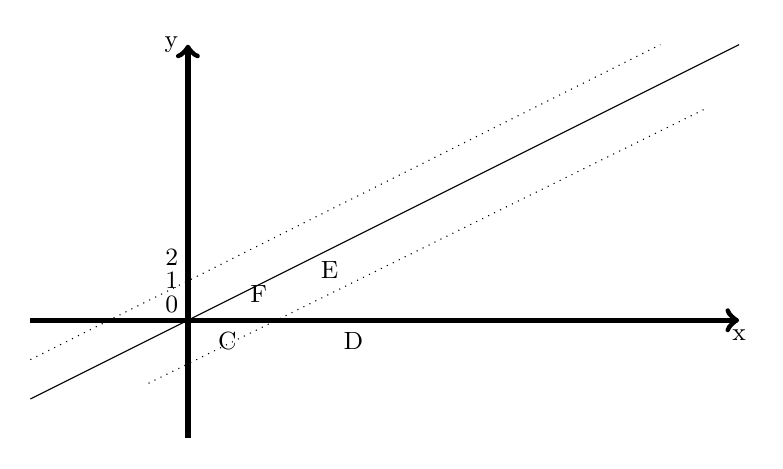
\begin{tikzpicture} [scale = 1]
\coordinate [label=left:\small{y}] (y) at (-3, 4);
\coordinate [label=below:\small{x}] (x) at (4, 0.5);
\coordinate [label=above:\small{C}] (C) at (-2.5, 0);
\coordinate [label=above:\small{D}] (D) at (-0.9, 0);
\coordinate [label=above:\small{E}] (E) at (-1.2, 0.9);
\coordinate [label=above:\small{F}] (F) at (-2.1, 0.6);
\coordinate [label=left:\small{0}] (0) at (-3, 0.7);
\coordinate [label=left:\small{1}] (1y) at (-3, 1);
\coordinate [label=left:\small{2}] (2y) at (-3, 1.3);
\draw[->, line width=2pt] (-5, 0.5) -- (4, 0.5);
\draw[->, line width=2pt] (-3, -1) -- (-3, 4);
\draw (-5, -0.5) -- (4, 4);
\draw[dotted] (-5, 0) -- (3, 4);
\draw[dotted] (-3.5, -0.3) -- (3.6, 3.2);
\end{tikzpicture}
\end{center}
\fi

%                                  62
Ведя речь об оценке универсальных выражений, справочник говорит\linebreak
в абзаце 4.10(4) ARM\footnote{
Ada Reference Manual, имеется перевод на русский язык: см. [186]. $-$\linebreak
\textit{Прим. перев.}
}:\newline
\hspace*{25pt}"$...Furthermore,$ $if$ $a$ $universal$ $expression$ $is$ $a$ $static$ $expression$,\newline
\hspace*{15pt}$then$ $the$ $evaluation$ $must$ $be$ $exact."$\footnote{
<<... Более того, если универсальное выражение $-$ статическое, то выраже-\linebreak
ние также должно быть точным.>> см. абзац 4.10.(4) в переводе ARM ([186]).$-$\linebreak
\textit{Прим. перев.}
}
\begin{center}
\textit{Статическая проверка непростоты $F_5$}
\end{center}
\begin{lstlisting}[mathescape=true, language=Ada, showstringspaces=false]
with $Text\_IO$; use $Test\_IO$;
procedure $Test\_Format\_s\_Number$ is
 $n : $ constant $:= 5$; $F_n :$ constant $:= 2 \ast\ast(2\ast\ast{n})+1$;--4_294_967_297
 
 $x_0 :$ constant $:= 5$; $x_1 :$ constant $:= (x_0 \ast\ast (2\ast\ast{6}))$
            mod $F_n$; -- $5 \ast\ast (2\ast\ast{6})$
 $x_2 :$ constant $:= (x_1 (\ast\ast 6))$ mod $F_n$; -- $5 \ast\ast (2\ast\ast{12})$
 $x_3 :$ constant $:= (x_2 (\ast\ast 6))$ mod $F_n$; -- $5 \ast\ast (2\ast\ast{18})$
 $x_4 :$ constant $:= (x_3 (\ast\ast 6))$ mod $F_n$; -- $5 \ast\ast (2\ast\ast{24})$
 $x_5 :$ constant $:= (x_4 (\ast\ast 7))$ mod $F_n$; -- $5 \ast\ast (2\ast\ast{31})$

begin
 if $x_5=F_{n-1}$ then $Put\_Line $("F_5 простое");
 else $Put\_Line$ ("F_5 составное");
 end if;
end $Test\_Fermat\_s\_Number$;
\end{lstlisting}
\hspace*{15pt}Отличительная  черта  этой  программы  заключается  в  том,  что  вы-\linebreak
числения  выполняются  в  описательной  части  программы,  с  использо-\linebreak
ванием  универсальных  целых  констант  (а  не  типизированных  целых\linebreak
констант).  Именно  при  компиляции,  а  не  во  время  выполнения,  оце-\linebreak
ниваются  все  выражеция.  По  вполне  понятным  причинам  невозможно\linebreak
прямо  вычислить $5^{\frac{F_5-1}{2}}$,  а  потом  взять  остаток  по  модулю  $F_5$ (кстати,\linebreak
сколько  десятичных  цифр  содержит  число  $5^{\frac{F_5-1}{2}}$?).  Итак,  вычисление\linebreak
разбито  на  части,  используя  статическую  и  улучшенную  версию  ди\linebreak
хотомического  возведения  в  степень.  Следовательно,  выполнение  про-\linebreak
граммы ограничивается обработкой результатов, полученных при ком-\linebreak
пиляции.
\begin{mynotice}
Помимо прочего, этот пример показывает, что лю-\linebreak
бой компилятор языка Ада обладает встроенным калькулятором\linebreak
произвольно большой точности (с точностью в пределах возмож-\linebreak
ностей конкретной машины), и можно только сожалеть, что этот\linebreak
\newpage
\noindent
калькулятор  не  доступен  при  выполнении  программ.  Разумеет-\linebreak
ся, таким способом можно проверить непростоту некоторых дру-\linebreak
гих чисел Ферма, если разлагать вычисления так тщательно, что-\linebreak
бы избежать  переполнения  разрядной  сетки компилятора  (числа\linebreak
Ферма растут  очень  быстро!)
\end{mynotice}
%                                  63
\section{4 Хорошее приближение к бесконечности}
\noindent
Все задачи в информатике можно условно разделить на два класса: за-\linebreak
дачи, имеющие решение, вычисляемое за разумное время, и задачи, ре-\linebreak
шение которых требует слишом большого времени вычисления. Изуче-\linebreak
ние многочисленных классов программ (или задач) составляет особую,\linebreak
самостоятельную область информатики,  названную \textit{теорией сложно-}\linebreak
\textit{сти} (книга D. Harel, $Algorithmics: The spirit of computing$
\footnote{
Д. Харел, Алгоритмика: Дух вычислений (англ.) $-$ \textit{Прим. перев.}}$-$ это увле-\linebreak
кательнейшее введение в эту теорию). Цель этого раздела $-$ доказать,\linebreak
что  некоторые  решения  простых  математических  задач  выходят  за\linebreak
рамки возможностей современных машин. Не делая чрезмерных обоб-\linebreak
щений, можно все же сказать, что эти решения никогда не будут вычи-\linebreak
сляться на машине, какой бы она ни была! Чтобы проиллюстрировать\linebreak
этот факт,  мы  решили  реализовать  вычисление  целочисленных  опре-\linebreak
делителей при помощи метода, исходящего прямо из математического\linebreak
определения детерминанта\footnote{
Впрочем, метод, вполне применимый (хотя, может быть, правильнее было бы\linebreak
сказать неприменимый) к вычислениям детерминантов, какова бы ни была природа\linebreak
элементов, т.е. для любого базового кольца.}. Итак, вот определение детерминанта, ко­
торое будет использоваться в этом разделе.
\begin{determ}
\hspace*{15pt}Пусть $A=(a_{ij})_{\substack{1\leqslant{i}\leqslant{n}\\1\leqslant{j}\leqslant{n}}}$ $-$ квадратная матрица с целыми элемен-\linebreak
тами. Детерминант (определитель) матрицы $A$, обозначаемый $|A|$ или\linebreak
$det{A}$ $-$ это число, определенное через $|A|=\sum_{\sigma\in{S_n}}\epsilon(\sigma)a_{1{\sigma(1)}}a_{2\sigma(2)}...$\linebreak
$a_{n\sigma(n)}$, где $S_n$ $-$ это множество перестановок интервала $[1,n]$, а $\epsilon$ $-$\linebreak
функция, дающая знак перестановки.
\end{determ}
Это определение  обладает  некоторой  инвариантной  эффективно-\linebreak
стью (по крайней мере, внешне): действительно, определитель, кажет-\linebreak
ся, может быть вычислен при помощи конечной суммы, любимой опера-\linebreak
ции в программах. Однако, прежде, чем приступить к программирова-\linebreak
нию этого метода, можно, а любой разумный человек должен, задать се-\linebreak
бе вопрос: сколько слагаемых имеет эта сумма? Математик тотчас же\linebreak
\newpage
%                                  64
\noindent
ответит: в этом выражении имеется, очевидно, $n!$ слагаемых (каждое\linebreak
состоит из $n$ множителей)! И обсуждение закончено. Но кто знает, ка-\linebreak
ково значение $n!$, когда $n$ принимает значения  10, 20, ..., т.е. значения\linebreak
очень скромные для любой  практической задачи,  имеющей матричное\linebreak
решение  (например,  задачи  метеорологии  или  моделирования течения\linebreak
жидкостей, где нередко приходится оперировать матрицами, имеющи-\linebreak
ми  тысячи  строк  и  столбцов)?  И  снова  математик  может  ответить,\linebreak
используя приближение Стирлинга, что
\begin{center}
$n!\approx n^ne^{-n}\sqrt{2\pi n}$ и даже $n!>n^ne^{-n}\sqrt{2\pi n}$,
\end{center}
а любая хорошая система алгебраического вычисления дает точные ре-\linebreak
зультаты:
\begin{center}
$10!=3 628 800$ и $20!=2 432 902 008 176 640 000$.
\end{center}
Последнее значение производит некоторое впечатление, оно приблизи­-\linebreak
тельно равно $2*10^{18}$. Зная, что современные микро-ЭВМ способны со-\linebreak
вершать  около  миллиона  сложений  в  секунду,  естественно  спросить:\linebreak
сколько времени затратит такой компьютер, чтобы выполнить $2*10^{18}$\linebreak
сложений?\newline
\hspace*{15pt}Этот пример без дополнительных выкладок не убеждает скептиков,\linebreak
которые считают,  что  стали  жертвами  фокуса.  Вот  по этой  причине\linebreak
мы и решили практически доказать сложность таких программ, взяв в\linebreak
качестве примера вычисление определителя.
\subsection{4.1 Элементы обработки массивов в языке Ада}
\noindent
Матрицы  обычно  представлены  в  алгоритмах  и  программах с  помо-\linebreak
щью массивов  (если  речь  не  идет о разреженных  матрицах,  для кото-\linebreak
рых в большинстве случаев представление оптимизируют). Кроме того,\linebreak
как мы увидим  в дальнейшем,  перестановки тоже можно представить\linebreak
с помощью этой структуры.  Следовательно, нужно изучить обработку\linebreak
массивов в языке Ада.\newline
\hspace*{15pt}Обработка массивов в языке Ада имеет только отдаленное отноше-\linebreak
ние к обработке, которую можно сделать в классических языках, таких\linebreak
как Паскаль, а средства, предоставленные в распоряжение пользовате-\linebreak
ля  разработчиками  языка,  удовлетворяют все  его  (разумные)  ожида­-\linebreak
ния.  Хотя  в  языке  Ада  и  невозможно  определить  массив  переменно-\linebreak
го размера, но существует понятие, позволяющее обрабатывать массив\linebreak
неизвестного  размера  во  время  построения  программы:  это  понятие\linebreak
\textbf{шаблона} (\textit{pattern} в англосаксонской терминологии).
\newpage
%                                  65
В качестве первой иллюстрации принципа шаблонов мы покажем,\linebreak
как в языке Ада построить процедуры или функции, число аргументов\linebreak
которых кажется переменным. Этот метод использования шаблонов не\linebreak
очень принят,  но дает блестящие результаты в задачах такого вида\linebreak
(см.  работу Буха [27]).  Выбранный нами этого пример является по-\linebreak
строением функции, позволяющей находить ее  наибольший аргумент\linebreak
(среди любого их количества). Для начала рассмотрим массив,  в ко­-\linebreak
тором множество индексов (подынтервал целых положительных чисел)\linebreak
и тип основных элементов произвольны. Массив называется $T$, а тип\linebreak
элементов массива $-$ $Object$. Так как мы ничего не знаем о типе элемен-\linebreak
тов, то если мы хотим вычислить максимум элементов массива, нужно\linebreak
располагать оператором сравнения; этот оператор обозначен <<$<$>>. Вы-\linebreak
числяемое значение $Max$ должно удовлетворять условию:
\begin{center}
при любом индексе $i$ массива $T$: $T(i)=Max$ или $T(i)<Max$.
\end{center}
В этом  выражении  внимательный  читатель  отметит  использование\linebreak
двух операторов,  <<$=$>>  и  <<$<$>>,  а не единственного оператора <<$\leqslant$>>:  про-\linebreak
граммистская шероховатость, которая будет сглажена при реализации\linebreak
этой функции в языке Ада.  Алгоритм вычисления  максимума очень\linebreak
прост, и нет необходимости его подробно объяснять. Итак, предлага-\linebreak
ем сразу реализацию этой функции в языке Ада, учитывая тот факт,\linebreak
что единственные допустимые операции на элементах типа $Object$ $-$\linebreak
это: описание, присваивание и сравнение оператором <<$<$>>.
\begin{lstlisting}[mathescape=true, language=Ada, frame=none, xleftmargin=20pt]
function $Max (T : Objects\_Array)$ return $Object$ is
 $Temporary\_Maximum : Object := T (T`First)$;
begin
 for $i$ in $T`First+1 .. T`Last$ loop
  if $Temporary\_Maximum<T(i)$ then $Temporary\_Maximum := T(i)$;
  end if;
 end loop;
 return $Temporary\_Maximum$;
end $Max$;
\end{lstlisting}
Основная характеристика этой части Ада-программы $-$ это полное от-\linebreak
сутствие явной ссылки на любое особое свойство обрабатываемого мас-\linebreak
сива: точно не известно, каковы индексы массива, и также не известны\linebreak
элементы, составляющие массив, а единственные используемые опера-\linebreak
ции $-$ это три операции, названные выше. Однако можно обработать\linebreak
массив, обработать его границы благодаря предопределенным функ-\linebreak
циям в языке Ада, которые называют \textit{атрибутами}. Таким образом,\linebreak
если $T$ $-$ массив, выражение $T`First$ обозначает наименьший  индекс\linebreak
массива $T$, a $T`Last$ обозначает наибольший индекс $T$. Это доказыва-\linebreak
\newpage

%                                  66
\noindent
ет, что функция, имеющая массив в качестве формального параметра,\linebreak
может каждый раз заново определять некоторые характеристики мас-\linebreak
сива,  который ей  передан  в качестве фактического параметра (длина,\linebreak
границы...):  атрибуты позволяют определить эти характеристики \textit{ди}-\linebreak
\textit{намически}, т.е. во время выполнения. Хотя это явно не выражено, но в\linebreak
этой  функции  используется  особое  свойство  индексов:  их  целочислен-\linebreak
ный характер, который позволяет записать выражение $T`First+1$.\newline
\hspace*{15pt}Логическое  следствие  всего  этого  заключается  в  том,  что  текст\linebreak
функции $Max$ всегда один и тот же и что обрабатываемые объекты $-$\linebreak
это  целые  числа,  действительные  числа,  литералы  перечисления  или\linebreak
любой другой объект при условии,  что пользователь задаст операцию\linebreak
сравнения. Другими словами, очень легко записать на основе всего ска-\linebreak
занного настраиваемый алгоритм вычисления максимума. Таким обра-\linebreak
зом, спецификация, обозначения которой слегка отличаются от преды-\linebreak
дущих, выглядит так:
\begin{center}
\textit{Спецификация настраиваемого алгоритма вычисления максимума}
\end{center}
\begin{lstlisting}[mathescape=true, language=Ada]
generic
    type $Object$ is private;
    with $Function "<" (a,b : Object)$ return $Boolean$ is $<>$;
package $Maximum$ is
    type $Objects\_Array$ is array $(Positive$ range $<>)$ of $Object$;
    function $Max (T : Objects\_Array)$ return $Object$;
end $Maximum$;
\end{lstlisting}
\hspace*{15pt}Рассмотрим сначала формальные  параметры  настройки  для этого\linebreak
пакета. Тип $Object$ $-$ это приватный тип; это означает, как мы видели\linebreak
в  разделе  3.3  (стр.  53),  что  единственными  операциями,  допустимы-\linebreak
ми неявно внутри пакета на объектах этого типа, являются описание,\linebreak
присваивание,  тест  на  равенство  и  использование  в  качестве  параме-\linebreak
тра  подпрограммы.  Следовательно,  разработчик  функции $Max$ ниче-\linebreak
го  не  знает  о  типе $Object$; он  не  может знать,  идет  ли  речь  о  целом\linebreak
типе,  последовательности  знаков...  Второй  формальный  параметр $-$\linebreak
это оператор сравнения элементов типа $Object$, необходимый для вычи-\linebreak
сления максимального значения,  но который невозможно прямо ввести\linebreak
из-за  незнания  типа $Object$. Кроме  того,  этот  формальный  параметр\linebreak
настройки  имеет  значение  по  умолчанию;  описание $\blacktriangleright$ \textbf{with function}\linebreak
$"<" (a,b : Object)$ \textbf{return} $Boolean$ is $<>; \blacktriangleleft$ означает,  что в случае,  ко-\linebreak
гда пользователь настраиваемого пакета не задает явно эту  функцию\linebreak
в момент конкретизации, то функция, которая должна быть использо-\linebreak
вана, — это функция $<$, имеющая соответствующий тип параметров и\linebreak
видимая в  месте  конкретизации.  Формальным параметрам настройки\linebreak
\newpage
%                                  67
\noindent
могут быть заданы другие виды значений по умолчанию, в дальнейшем\linebreak
мы еще с ними встретимся.\\

Имея эти два параметра, разработчик функции $Max$ задает пользо-\linebreak
вателю, с одной стороны, тип $Objects\_Array$, который, в основном, не\linebreak
будет использоваться,  и функцию $Max$, которая нас интересует.  Тип\linebreak
$Objects\_Array$ служит только для описания типа параметров функции\linebreak
$Max$. Как будет видно в применении функции, пользователь может его\linebreak
полностью игнорировать. Описание типа $Objects\_Array$ $-$ это несколько\linebreak
своеобразное описание массива: $\blacktriangleright$ \textbf{type} $Objects\_Array$ \textbf{is array} $(Positive$\linebreak
\textbf{range}<>$)$ \textbf{of} $Object;\blacktriangleleft$. Это будет точное описание шаблона, и говорить\linebreak
о типе, имеющем отношение к идентификатору $Object\_Array$, значит\linebreak
злоупотреблять языком. Действительно, невозможно описать перемен-\linebreak
иые типа $Object\_Array$, потому что Ада, как любой другой язык, дол-\linebreak
жен иметь возможность предоставить в памяти место, необходимое для\linebreak
массива. Впрочем, вполне возможно использовать этот шаблон для опи-\linebreak
сания типа формальных параметров подпрограммы: при фактическом\linebreak
использовании подпрограммы ее параметрами будут описанные пере-\linebreak
менные (обратное было бы удивительным) или выражения, построен-\linebreak
ные в момент вызова, характеристики которых хорошо известны, когда\linebreak
контроль идет внутри подпрограммы.\\

Тело пакета $Maximum$ записывается прямо, непосредственно и явля­-\linebreak
ется, по существу, ни чем иным, как переформулировкой функции $Max$,\linebreak
представленной выше.
\begin{center}
\textit{Реализация функции Max}
\end{center}
\begin{lstlisting}[mathescape=true, language=Ada, xleftmargin=15pt]
package body $Maximum$ is
 function $Max (T : Objects\_Array)$ return $Object$ is
  $Temporary\_Maximum : Object := T (T`First)$;
 begin
  for $i$ in $T`First+1 .. T`Last$ loop
   if $Temporary\_Maximum < T(i)$ then $Temporary\_Maximum := T(i);$ end if;
  end loop;
 return $Temporary\_Maximum$;
 end $Max$;
end $Maximum$;
\end{lstlisting}
\hspace*{15pt}Перейдем теперь к использованию этой функции. Неинтересно по-\linebreak
дробно объяснять всю программу, использующую эту функцию (в са-\linebreak
мом деле, длина такой программы была бы огромной по сравнению с\linebreak
необходимым пояснением функции $Max$), однако несколько фрагментов\linebreak
такой программы разъяснят возможности функции.
\newpage
%                                  68
\begin{lstlisting}[mathescape=true, language=Ada, frame=none, xleftmargin=15pt]
with $Maximum;--$ Продолжение контекста компиляции
procedure $Using\_Function\_Max$ is
 type $My\_Integer$ is $...-- \text{ В этом месте уже определен оператор "<"}$
                         $\text{на целых числах типа Integer}$
 package $Integer\_Maximum$ is new $Maximum (My\_Integer)$;
                         use $Integer\_Maximum$;
 $x , a , b , c , d : My\_Integer;--\text{Продолжение описаний(переменные ...)}$
begin
 $--\text{ Начало вычислений}$
 $x := Max ((a,b,c));--\text{ Продолжение вычислений}$
 $x := Max ((a,b,c,d));--\text{ Конец вычислений}$
end $Using\_Function\_Max$;
\end{lstlisting}
\hspace*{15pt}Эта программа использует конкретизацию пакета $Maximum$ для це-\linebreak
лых чисел; как видим, она начинается с оператора контекста (может\linebreak
быть неполного в примере), ссылающегося на настраиваемый пакет.\linebreak
Внутри главной процедуры после определения  целого типа, который\linebreak
наследует обычные операции на целых числах, и в частности, опера-\linebreak
тор сравнения <<$<$>>, находим конкретизацию настраиваемого пакета, в\linebreak
которой задан только фактический параметр, соответствующий типу\linebreak
$Object$; так как второй параметр явно не задан, при конкретизации для\linebreak
него используется значение по умолчанию, т.е. стандартный оператор\linebreak
<<$<$>> сравнения целых чисел. Можно уже заметить, что если бы вместо\linebreak
использования оператора <<$<$>> передали  в качестве второго параметра\linebreak
оператор <<$>$>>, как в команде
\begin{lstlisting}[mathescape=true, frame=none, language=Ada, xleftmargin=15pt]
package $Integer\_Minimum$ is new $Maximum (My\_Integer, ">")$;
\end{lstlisting}
то построенная таким образом функция $Max$ вычислила бы наименьший\linebreak
из своих аргументов, а не наибольший.\newline
\hspace*{15pt}После спецификатора видимости $\blacktriangleright$ \textbf{use} $Integer\_Maximum \blacktriangleleft$ и не-\linebreak
скольких дополнительных описаний находим тело главной процедуры,\linebreak
которое содержит определенное количество дополнительных вычисле-\linebreak
ний и (что нас интересует) два обращения к функции $Max$:
\begin{lstlisting}[mathescape=true, language=Ada, frame=none, xleftmargin=15pt]
$x:=max ((a,b,c)); x:=max ((a,b,c,d))$;
\end{lstlisting}
Выражения,  которые  образуют  фактические  параметры  этих  двух\linebreak
обращений,  являются \textit{агрегатами}, т.е.  явными  структурными\linebreak
конструкциями.  Фактический  параметр первого обращения  к функ-\linebreak
ции $Max$ $-$ это агрегат $(a,b,c)$, который вне своего контекста пред­-\linebreak
ставляет структуру с тремя компонентами типа $My\_Integer$. Это вы-\linebreak
ражение  (агрегат) совместимо с точки зрения типа как с записью с\linebreak
тремя полями типа $My\_Integer$, так и с индексируемым типом с тремя\linebreak
компонентами,  индексы  которого абсолютно произвольны.  Контекст\linebreak
\newpage
%                                  69
\noindent
использования  этого  агрегата  определяет  точным  образом  тип  выра-\linebreak
жения $(a,b,c)$: так как это параметр функции $Max$, то мы имеем  дело с\linebreak
индексируемым  типом  с  тремя  компонентами  (потому  что  в  агрегате\linebreak
их три),  индексированным посредством подынтервала типа $Positive$. О\linebreak 
нем  больше  ничего  не  известно,  и  точное  определение  данного  интер-\linebreak
вала  не  представляет  здесь  никакого  интереса  (за  дополнительными\linebreak
сведениями читатель может обратиться к $ARM$). В этих условиях вто-\linebreak
рой  вызов  функции $Max$ существенно  не  отличается  от  первого:  эта\linebreak
функция  может  применяться  к  массивам  любой  длины,  и  если  бы  не\linebreak
перегруженность  скобками,  то  можно  было  бы  сказать,  что  функция\linebreak
$Max$ обладает переменным  числом  параметров.\newline
\hspace*{15pt}Теперь  должно быть ясно,  что  пользователю этой  функции  нет  не-\linebreak
обходимости представлять тип $Objects\_Array$ в программе; один из слу-\linebreak
чаев, когда это будет необходимо, соответствует использованию функ-\linebreak
ции $Max$, применяемой к \textit{переменной} индексируемого  типа,  но это уже\linebreak
другая  история...
\subsection{4.2 Работа с матрицами}
\noindent
Следующий этап обучения обработке массивов в языке Ада заключает-\linebreak
ся  в  изучении  представления  матриц,  базовых операций  над  матрица-\linebreak
ми,  ввода-вывода  матриц  $-$  короче,  в  определении  так  называемого\linebreak
\textbf{абстрактного  типа  данных} и  в  построении  нескольких  средств\linebreak
управления  такого типа.\newline
\hspace*{15pt}Первая  фаза $-$  определение  абстрактного  типа  данных $-$ начина-\linebreak
ется с распознавания того, что называют простейшими  операциями на\linebreak
типе.  Сначала можно отметить,  что эти  операции  подразделяются  на\linebreak
два вида: \textbf{конструкторы } и \textbf{селекторы}\footnote{
Эта терминология кажется повсюду принята программистами, она произо-\linebreak
шла из разработки технологии программного обеспечения. Можно обратиться к\linebreak
книге Буха $[27]$, которая дает более полные определения с последующим стилем\linebreak
программирования.}. Конструкторы $-$ это опера-\linebreak
ции,  которые  модифицируют состояние  (значение)  данных,  тогда как\linebreak
селекторы  позволяют только узнать это состояние.\newline
\hspace*{15pt}Каковы  же  будут фундаментальные операции,  когда объект $-$  ма-\linebreak
трица?  Прежде  всего,  имеется  конструктор,  который  позволяет  при-\linebreak
сваивать значение элементу матрицы,  а также симметричная операция\linebreak
селектор,  позволяющий  узнать  значение  одного  из  элементов.  Напри\linebreak
мер,  если $A - $ рассматриваемая  матрица,  а $a_{ij}-$ интересующий  нас\linebreak
элемент, то обычно обозначаем $A(i,j)\longleftarrow v$ и $v\longleftarrow A(i,j)$ те действия,\linebreak
которые реализуют эти операции. Но такой способ действия имеет мно-\linebreak
\newpage

%                                  70
\noindent
го последствий и, в частности, приводит к тому, что матрицы всегда\linebreak
представляются с помощью массивов. Однако хорошо известно, что это\linebreak
не так! Некоторые матрицы $-$ разреженные: матрицы, у которых толь-\linebreak
ко небольшое количество элементов не равно нулю; было бы совершенно\linebreak
неразумно, с точки зрения информатики, представлять матрицу боль-\linebreak
ших размеров, например, $1000\times 1000$, с помощью массива в миллион\linebreak
клеток, если всего лишь 10000 элементов не равны нулю. Следователь-\linebreak
но,  если  все  программы,  составленные  для  работы  с  матрицами, ис-\linebreak
пользуют понятие индексируемого типа, то эти программы становятся\linebreak
полностью непригодными, когда хотят применить их алгоритмы к раз-\linebreak
реженным матрицам. Иначе говоря, программы слишком зависимы от\linebreak
внутреннего представления обрабатываемых объектов.\newline
\hspace*{15pt}Конкретно, этот тип  представления обязывает программиста вы-\linebreak
ражать присваивание и оценку элемента матрицы, соответственно, по-\linebreak
средством вызова процедуры и функции, даже если это, возможно, бу-\linebreak
дет тяжелее записывать (что справедливо лишь отчасти). Конструктор\linebreak 
обозначен $Set\_Coefficient$, а селектор $- Coefficient\_Of$ со спецификаци-\linebreak
ями, которые мы увидим в пакете, представленном далее.\newline
\hspace*{15pt}Этих двух операций недостаточно, чтобы выполнить все возможные\linebreak
манипуляции на матрице; не хватает селекторов, позволяющих узнать\linebreak
размер матриц, чтобы знать, какие элементы существуют. Так как тон-\linebreak
кая структура матрицы совершенно не известна пользователю матрицы\linebreak
(но не разработчику, роль которого мы сейчас выполняем), невозможно\linebreak
использовать различные атрибуты массива, как в предыдущем разделе\linebreak
а нужно явно задать функции, позволяющие оценить границы матри-\linebreak
цы: $First\_Row, Last\_Row, First\_Column, Last\_Column$.\newline
\hspace*{15pt}Чтобы модуль был как можно более автономным, нужно предусмо-\linebreak
треть  и  классифицировать  возможные ошибки  и  сопоставить им ис-\linebreak
ключения.  В случае матрицы единственная ошибка обработки $-$ это\linebreak
ссылка  на  несуществующий  элемент;  эту  ошибку  символизирует  ис-\linebreak
ключение $Index\_Out\_Of\_Bounds$, которое может появиться только при\linebreak
выполнении простейших операций $Set\_Coefficient$ и $Coefficient\_Of$.\newline
Вот полная спецификация настраиваемого пакета, реализующего аб-\linebreak
страктный тип данных.
\begin{center}
\textit{Матрица с целыми элементами}
\end{center}
\begin{lstlisting}[mathescape=true, language=Ada, frame=lrt]
generic
 type $Row\_Index$ is range <>;
 type $Column\_Index$ is range <>;
 type $Coefficient$ is range <>;
\end{lstlisting}
\newpage
%                                  71
\begin{lstlisting}[mathescape=true, language=Ada, frame=lbr]
package $Matrix\_Nonsparse\_Integer$ is
 type $Matrix (First\_Row : Row\_Index; Last\_Row : Row\_Index;$
      $First\_Column : Column\_Index; Last\_Column : Column\_Index)$ is private;
 procedure $Set\_Coefficient (Of\_The\_Matrix :$ in out $Matrix$;
                     $At\_Row :$ in $Row\_Index$;
                     $And\_Column :$ in $Column\_Index$;
                     $To\_The\_Value :$ in $Coefficient)$;
 function $Coefficient\_Of (The\_Matrix : Matrix$;
                     $At\_Row : Row\_Index$;
                     $And\_Column : Column\_Index)$ return $Coefficient$;            
 function $First\_Row (Of\_The\_Matrix : Matrix)$ return $Row\_Index$;
 function $Last\_Row (Of\_The\_Matrix : Matrix)$ return $Row\_Index$;
 function $First\_Column (Of\_The\_Matrix : Matrix)$ return $Column\_Index$;
 function $Last\_Column (Of\_The\_Matrix : Matrix)$ return $Column\_Index$;
 
 $Index\_Out\_Of\_Bounds :$ exception;
 
private
 type $Matrix\_Template$ is
     array$(Row\_Index$ range <>,$Column\_Index$ range <>$)$ of $Coefficient$;
 type $Matrix (First\_Row : Row\_Index; Last\_Row : Row\_Index;$
            $First\_Column : Column\_Index; Last\_Column : Column\_Index)$
 is record
  $The\_Coefficient :$
     $Matrix\_Template (First\_Row .. Last\_Row, First\_Column .. Last\_Column)$;
 end record;
 pragma $Inline (Set\_Coefficient, Coefficient\_Of,$
             $First\_Row, Last\_Row, First\_Column, Last\_Column)$;
end $Matrix\_Nonsparse\_Integer$;
\end{lstlisting}

Первое замечание касается имени пакета, $Matrix\_Nonsparse\_Integer$.\linebreak
В  этом  имени  соблюдаются  простейшие  правила  построения:  первый\linebreak
радикал означает,  что  абстрактный  тип  данных,  который в  нем  опре-\linebreak
делен, $-$ матрица, второй, что эти матрицы не разреженные  (алгорит-\linebreak
мы  доступа  к  разреженным  матрицам,  в  основном,  другие),  и,  нако-\linebreak
нец, суффикс указывает на тип элементов. Это имя позволяет сразу же\linebreak
узнать примерные характеристики  определенного объекта\footnote{
Эта  проблема  может  показаться  устаревшей,  но  в  программировании  выбор\linebreak
идентификаторов $-$ важная и  тонкая операция, и  некоторые труды по  разработке\linebreak
технологии программного обеспечения посвящают этой проблеме целую  главу.}.\newline
Рассмотрим теперь видимую часть этой спецификации  (т.е.  все то,\linebreak
что предшествует  ключевому слову \textbf{private}). Прежде  всего,  формаль-\linebreak
%                                  72
\noindent
ных параметров  настройки  три  и  их  семантика  должна  быть ясной...\linebreak
Читатель педантичный  (и усидчивый, см. раздел 3.3) сможет нас упрек­-\linebreak
нуть  в  том,  что мы  не  определили,  что элементы  — личного типа  (т.е.\linebreak
почти  любого),  это  позволило  бы  обрабатывать одинаковым  способом\linebreak
матрицы  целых  чисел,  чисел  с  плавающей  запятой,  многочленов и  т.д.\linebreak
Этот выбор  основан  на  том,  что  обычно  не  совершают  один  и  тот же\linebreak
тип  вычислений  и  на матрицах с целыми  и  на  матрицах с  действитель­-\linebreak
ными  элементами  и  что  алгоритмы  вычисления  на  матрицах  много­-\linebreak
членов  не являются  простым  применением  в  кольце  многочленов  алго­-\linebreak
ритмов  для  матриц  с  элементами  из  числового  кольца.  Другими  сло­-\linebreak
вами,  алгоритмы  вычисления  на  алгебраических  структурах  соответ­-\linebreak
ствуют  структурному  типу,  который  подлежит  обработке.  Например,\linebreak
если $A-$ матрица и  если a мы хотим вычислить $A^n$,  то  для этого можно\linebreak 
взять  великолепную  настраиваемую  функцию  дихотомического  возве­-\linebreak
дения в степень,  изученную в разделе 3.3; но намного более экономично,\linebreak
при условии,  что $n-$ достаточно большое, вычислить характеристиче-\linebreak
ский  многочлен (или  минимальный,  если  умеем  его  вычислять) от $A$  и\linebreak 
прежде,  чем  вычислить  произведения  матриц,  привести  $A^n$  по  модулю \linebreak
этого  многочлена.  Все  эти  примеры  показывают,  что  можно  фиксиро­-\linebreak
вать  тип  элементов  матрицы:  что  теряем  в  общем,  то  выигрываем  в\linebreak
полезном...\\

Собственно  спецификация  начинается  с  определения  личного  типа\linebreak
$Matrix$, который обладает четырьмя дискриминантами с красноречивы-\linebreak
ми  именами.  Когда этот пакет  получит  начальные значения, тогда бу-\linebreak
дет возможно описать, например, переменную $\blacktriangleright A:Matrix(2,4,3,7);\blacktriangleleft$
это  означает,  что  $A-$ это  матрица  $3\times 5$,  у  которой  индексы  строчек\linebreak 
находятся  в  интервале  $[2,4]$,  а  индексы  столбцов  $-$  в  интервале  $[3,7]$.\linebreak 
Конкретизация  этого  пакета  порождает  не  единственный  матричный\linebreak
тип, а, скорее,  класс матриц, имеющих некоторые общие характеристи-\linebreak
ки  (тип  индексов  и  конкретный  тип  элементов).  Преимущество  этого\linebreak
способа  действия  состоит  в  том,  что  он  позволяет  обрабатывать  ма-\linebreak
трицы  различных  размеров,  исходя  только из  начальных значений.\\

Перейдем  теперь  к  точному  определению  типа $Matrix-$ определе-\linebreak
нию,  которое  обычному,  среднему  пользователю знать  необязательно.\linebreak 
Так  как  реализуются  <<полные>>  матрицы,  внутреннее  представление  ис-\linebreak
пользует  двумерные  массивы.  Но  синтаксис  языка  Ада  предписывает,\linebreak
чтобы  определение  типа,  фигурирующее  в  личной  части,  имело  то же\linebreak
начало,  что присутствует  у  него  в спецификации.  Следовательно, этот\linebreak
тип  должен  быть  типом  дискриминанта  записи,  его  единственное  по-\linebreak
ле  (отличное от  дискриминантов)  $-$ это двумерный  массив,  о котором\linebreak
\newpage


%%\documentclass{../../template/mai_book}
%\defaultfontfeatures{Mapping=tex-text}
%\setdefaultlanguage{russian}
%\begin{document}
мы говорили. На распечатке спецификации можно увидеть определения
типов, которые должны быть представлены в личной части.
Все это может показаться невероятно сложным и неэффективным.
Это действительно сложно для того, кто не имеет достаточного опыта
в программировании. Эта сложность кажется бесполезной тому, кто
никогда не пытался повторно использовать свои программы в контек­
стах, слегка отличных от контекста разработки: с опытом приходит
понимание, что эту цену необходимо платить один только раз — лишь
во время первого написания. Некоторые могут еще сослаться на то,
что теряется четкость: пишем \textit{►~Set-Coefficient (A, i, j,\dots)~◄} вместо
\textit{►~A(i,j) := \dots~◄}. И опять, все это вопрос опыта: если стиль — однород­
ный, программы читаются так же легко, как и программы, записанные
обычным способом.
В том, что касается эффективности, язык Ада предоставляет нам
некоторые средства, позволяющие влиять на скорость выполнения про­
грамм или на объем их памяти. Для этого компилятору передаются
указания, называемые прагмами. Возможно, что эти указания будут
безрезультатны (это зависит от используемого компилятора), но не со­
ставит большого труда их предусмотреть. Как это можно увидеть в
личной части, прагма Inline — которая указывает, что обращения к
подпрограммам \textit{Set-Coefficient, Coefficient-Of,\dots} нужно развернуть «в
строке», т.е. заменить обращения к этим подпрограммам разложением
их тела, — применима для всех простейших операций этой специфика­
ции.
Вторая фаза определения типа \textit{Matrix} — его реализация, очень про­
стая операция. Действительно, внутренняя структура представляет со­
бой двумерный массив, реализация примитивов — это перезапись про­
цедур и функций спецификации в терминах массивов. Вместо долгих
объяснений проще прямо представить тело пакета.

\begin{lstlisting}
typedef double value_T;
struct _matrix_T {
    int n, m;
    value_T *body;
}
typedef struct _matrix_T *matrix_T;

bool set_coefficient(matrix_T mat,
                     row_T row,
                     column_T col,
                     value_T val) {
    int mat_i = TO_COEFFICIENT(row, col);
    if (mat_i > mat->max_i) {
        // Exception Handler...
        return false;
    }
    mat->body[mat_i] = val;
    return true;
}
value_T* last_row(matrix_T mat) {
    size_t m = mat->m;
    size_t n = mat->n;
    return mat->body + (n-1)*m;
}

value_T* last_col(matrix_T mat) {
    size_t m = mat->m;
    size_t n = mat->n;
    return mat->body + m;
}

value_T* next_col(matrix_T mat, value_T *cur_col) {
    return cur_col + mat->m;
}

value_T* next_row(matrix_T mat, value_T *cur_row) {
    return cur_row + mat->n;
}

\end{lstlisting}

Можно сразу отметить простоту кода (нельзя по-настоящему го­
	ворить об алгоритме), но, тем не менее, нужно уточнить несколько
моментов. При определении типа мы представили некоторые ошибки,
которые могут появиться при использовании этого пакета. Следова­
тельно, надо выявить эти ошибки в теле имеющих к этому отношение
простейших операций. Для этого существует несколько способов:


\begin{itemize}  
\item в начале каждого модуля, в котором может появиться ошибка,
выполняют тест, позволяющий узнать, не произойдет ли ошибка.
Для этого нужно уметь предусмотреть все потенциальные ошибки
и надо уметь распознавать их предпосылки, что не всегда легко
и возможно;
\item другое решение состоит в том, чтобы использовать механизм ис­
ключений языка Ада, т.е. дать возможность модулям следовать
\newpage
обычному ходу их выполнения и предусмотреть в конце модуля
обработчик исключений, восстанавливающий предопределенные
исключения и распространяющий одно из исключений, которое
было определено для этого типа данных. Это второе решение,
заранее привлекательное из-за своей эффективности, — в неко­
торых реализациях языка Ада обработка исключений не требует
дополнительных издержек, пока не появятся исключения — имеет
то т недостаток, что не гарантирует связности данных. В случае
матриц, как они были только что реализованы, эта проблема не
требует особого внимания.
\end{itemize}

Исключение представляет собой асинхронное или непредусмотрен­
ное событие, которое может вызвать прекращение обработки информа­
ции, обеспечивающей связанность некоторых данных. Например, при
реализации динамических структур, связность которых обеспечивает­
ся указателями, очень важно, чтобы ошибки не возникали в момент,
когда связи между структурами несогласованы, что часто происходит
при модификациях. Если это возможно, нужно обязательно выявить по­
тенциальные ошибки перед их появлением, и следовательно, применить
первый метод.
Вновь эти проблемы возникают потому, что от пользователя хотят
скрыть истинное представление обрабатываемых объектов, при этом
маскирование информации доходит до утаивания внутренних ошибок!
Итак, находим обработчики исключений в реализации двух эле­
ментарных операций Set-Coefficient и Coefficient.Of: предопределенное
исключение Constraint-Error, возбуждаемое в случае ошибки выхода
индекса матрицы за его пределы, устраняется и далее распростра­
няется исключение Index-Out-Of-Bounds. Выполнение четырех неболь­
ших примитивов, позволяющих узнать границы матрицы, не может
вызвать ошибку, следовательно, там не должно быть никакой обра­
ботки ошибки. Мы уже встречали атрибуты, действующие на масси­
вах, в разделе 4.1, и в этих последних функциях снова находим атри­
буты First и Last, это показывает, каким образом данные атрибуты
применяются в случае многомерного массива, например, в ► re tu rn
Of-The-Matrix.The.Coefficient’First (1), < параметр атрибута First ука­
зывает номер размерности, к которой применяется First.

\begin{mynotice}
Хотя только что изученные операции на матрицах
являются, действительно, единственными элементарными опера­
циями, может случиться, что в эту спецификацию добавят опе­
рации, которые очень часто используются. Это в большинстве
\newpage
случаев очень простые операции, но которые по причинам эффек­
тивности и простоты выигрывают за счет информации о точном
представлении данных.
\end{mynotice}

\subsection{Ввод-вывод матриц}

Второй модуль обработки матриц позволит нам научиться использо­
вать один тип абстрактных данных. Для задачи, которая нас сейчас
занимает, первым необходимым нам инструментом является множе­
ство функций ввода-вывода. Такой аппарат содержит, как минимум,
процедуру чтения Get и процедуру записи Put для терминала, которых
пока достаточно.
Эти две процедуры предоставляют минимальное удобство для поль­
зователя: Put имеет параметр, позволяющий задать размер поля для
вывода элементов матрицы, которую хотят вывести; a Get имеет па­
раметр, который задает выводимое для ввода одной строки матрицы.
У этих двух параметров есть, однако, одна особенность: они имеют
значение по умолчанию. Благодаря этому, если выполняется команда
► Get (Моя-Матрица);
при отсутствии второго параметра в вызове,
программа будет использовать его значение по умолчанию, и никако­
го приглашения при чтении матрицы не появится. Зато если уточнить
► Get (Моя-Матрица,
◄ , каждое чтение одной строки будет
предваряться вопросительным знаком, позволяя пользователю знать,
где он находится. Значение по умолчанию второго параметра проце­
дуры Put есть Coefficient ’Width, результат применения предопределен­
ного атрибута Width к целому типу Coefficient: этот атрибут задает
максимальное число символов для вывода какой-либо величины типа
Coefficient.
После того как описаны средства, предлагаемые модулем, т.е. услу­
ги, которые он способен предоставить, нужно познакомиться и с услу­
гами, в которых он нуждается, чтобы реализовать все это. Эти услу­
ги появятся в качестве формальных параметров настройки и должны
быть обеспечены предыдущим пакетом. Тогда получится следующая
полная спецификация:

\begin{lstlisting}
bool set_coefficient(matrix_T mat,
                     row_T row,
                     column_T col,
                     value_T val) {
    int mat_i = TO_COEFFICIENT(row, col);
    if (mat_i > mat->max_i) {
        // Exception Handler...
        return false;
    }
    mat->body[mat_i] = val;
    return true;
}
value_T* last_row(matrix_T mat) {
    size_t m = mat->m;
    size_t n = mat->n;
    return mat->body + (n-1)*m;
}
value_T* last_col(matrix_T mat) {
    size_t m = mat->m;
    size_t n = mat->n;
    return mat->body + m;
}
value_T* next_col(matrix_T mat, value_T *cur_col) {
    return cur_col + mat->m;
}
value_T* next_row(matrix_T mat, value_T *cur_row) {
    return cur_row + mat->n;
}
bool put(matrix_T mat, size_t row, size_t col, value_T val) {
    int mat_i = TO_COEFFICIENT(row, col);
    if (mat_i > mat->max_i) {
        // ERROR HANDLER
        return false;
    }
    mat->body[mat_i] = val;
    return true;
}
value_T get(matrix_T mat, size_t row, size_t col) {
    int mat_i = TO_COEFFICIENT(row, col);
    if (mat_i > mat->max_i) {
        // ERROR HANDLER
        return mat->body[0];
    }
    return mat->body[mat_i];
}
\end{lstlisting}
«Это не упрощает дела!» — сразу скажет читатель. Еще раз по­
вторим сказанное: только опыт позволит судить об этом, и во время
заключительного построения будет видно, что описанный способ дей­
ствия имеет, скорее, тенденцию к упрощению архитектуры программы.
Однако сделаем несколько уточнений:
\begin{itemize}
\item процедуры ввода-вывода нуждаются в информации о типе Ma­
trix, и поскольку он определен как личный тип, то здесь он тоже
должен быть объявлен личным;
\item для считывания и записи должны быть известны границы обра­
батываемых матриц, так же как и природа элементов, ибо, в ко­
нечном счете, именно над ними производятся действия; это объ­
ясняет присутствие первых четырех параметров настройки;
\item наконец, нужно ввести все примитивы, определенные в предыду­
щем разделе.
\end{itemize}

Данная спецификация, которая кажется довольно громоздкой, полна
и очень мало связана с другими модулями. Это означает, что исполь­
зовать указанный модуль весьма просто и что модификации описания
типа абстрактных данных Matrix или других тяготеющих к нему мо­
дулей мало скажутся на этом особом модуле.

Приводим реализацию описанной процедуры, которая пока не пред­
ставляет никакой особой трудности.
\begin{lstlisting}
bool get_all(matrix_T mat) {
	for (size_t i = 0; i < mat->max_i; ++i)
		put(mat, m, n, get_val());
	return true;
}
\end{lstlisting}

Отметим способ, с помощью которого здесь используются примити­
вы работы с матрицами, а также ассоциацию по именам фактических
параметров самих этих примитивов. Сделаем последнее замечание, ка­
сающееся имени рассмотренного пакета: что хоть и следует избегать
этого в общем случае, в данном идентификаторе используют аббреви­
атуру 10 — общепринятый акроним, означающий Input/Output, как,
например, в TextJO.

\subsection{Описание генератора биекций}

Перейдем теперь к вычислению определителя матрицы, пользуясь фор­
мулой определения 7 в начале раздела 4 и предполагая, что мы обладаем

\newpage

генератором биекций между двумя целыми интервалами. Реализация
самого генератора отнесена в конец главы, чтобы не отвлекаться от
нашей первоначальной задачи.
Даже если на время не стоит вопрос о деталях построения генера­
тора перестановок, нужно, по крайней мере, знать способ его примене­
ния и инструменты, которые он предлагает, — короче, его описание.
Первый шаг на этом пути — выбор структуры данных, допускающей
представление одной перестановки. Существует несколько стандарт­
ных обозначений для перестановок: в форме произведения циклов, в
форме таблицы, представляющей граф перестановки, и т.п. Например,
перестановка $\delta$ интервала [1,5], определенная равенствами $\delta(1)~=~2,
\delta(2) = 4, \delta(3) = 5, \delta(4) = 1 и \delta(5) = 3$, представляется в форме про­
изведения циклов как: $\delta = ( 1 2 4 )( 3 5 )$, а в форме таблицы, как
$\delta = \begin{pmatrix} 1 & 2 & 3 & 4 & 5 \\ 2 & 4 & 5 & 1 & 3 \end{pmatrix} $
Этот второй способ представления дает более
непосредственный взгляд на перестановку (по крайней мере, на нашем
уровне) и больше подходит для алгоритмической обработки, чем запись
через произведение циклов. Обычно это представление упрощают, за­
писывая только вторую строку таблицы и подразумевая первую. По
этому соглашению перестановка сг предыдущего примера представля­
ется пятеркой (2,4,5,1,3).
Выбрав структуру данных, остается найти процедуру перебора
множества перестановок. Канонический метод просмотра конечного
множества состоит в полном его упорядочении от минимального (со­
ответственно, максимального) элемента для этого порядка и функции
следования (соответственно, предшествования). Вот описание настра­
иваемого пакета, определяющего такой генератор.

\newpage
\begin{lstlisting}

typedef enum {
\\ ...
} source;

typedef enum {
\\ ...
} target;

typedef enum {
\\ ...
} signature;

typedef target bijetion[RANGE];
bijection min_bij(source s_min,
				  source s_max, 
				  target t_min,
				  target t_max);
inline void sucsessor_of(bijection bij, signature sig);

\end{lstlisting}
% TODO: code

Э тот модуль определяет, кале указывает его имя, генератор биек­
ций, а не перестановок. Разница между двумя понятиями очень незна­
чительна, но рассмотрение биекций допускает, как увидим во время
реализации, более простой подход. Заглавные параметры этого моду­
ля суть типы (целые) интервалов от начальной точки до конечной, на
которых действует биекция. В нашем случае эти интервалы будут ин­
тервалами изменения индексов строки и столбца обрабатываемой ма­
трицы. С помощью этих двух типов целых программа выдаст нам так­
же два типа: один, позволяющий представить перестановки в форме
таблицы, другой — тип-сигнатуру. Затем, основывая принцип перечи­
сления биекций на некотором порядке, используют функцию, опреде­
ляющую наименьшую биекцию относительно этого порядка, и проце­
дуру вычисления последующей за данной биекции, а также ее сигна­
туру. Когда обрабатывают перестановки, наименьшей перестановкой
в выбранном порядке является тождественная, как это увидим ниже,
чья сигнатура равна 1; это указывает инициализацию, которую должна
осуществить программа вычисления детерминанта. Тогда можно легко
перебрать множество биекций между двумя интервалами целых чисел.
Возможны две ошибки. Bijection.Overflow выполняется, когда пытают­
ся вычислить биекцию, которая следует за самой большой в выбранном
порядке; и вторая — если пытаются вычислить минимальную биекцию
между двумя множествами с разными мощностями.

\subsection{Вычисление определителя}
Чтобы достичь нашей цели — вычисление определителя — остается
только объединить множество небольших кусков, которые мы постро­
или до сих пор: матричный тип, ввод-вывод, генератор перестановок и
написать, собственно, подпрограмму вычисления.
Матрицы, которые мы будем обрабатывать, — квадратные, с целы­
ми элементами, и мы будем предполагать, что индексы строк и столб­
цов имеют то т же тип. Когда этот выбор сделан, нужно конкрети­
зировать оба настраиваемых пакета по оперированию с матрицами и

вступить в диалог с пользователем. Именно это делает первый модуль
программы, представленный здесь:

% TODO: code
\begin{lstlisting}
typedef unsigned int index;
typedef long long int coefficient;
void compute_determ

while (true){
	size_t size;
	scanf("%d", &size);
	matrix mat;
	get_all(mat);
}
\end{lstlisting}

Начинают, таким образом, с построения матричного типа и его
примитивов; тогда можно конкретизировать пакет ввода-вывода ма-
\newpage
триц (эта последняя конкретизация довольно громоздка для записи)
Конкретизация пакета Integer.IO позволяет считывать размер матри­
цы, подлежащей обработке. Это чтение размера находится в основное
цикле, который содержит также блок, в котором объявляют матри­
цу, считывают ее элементы и проводят вычисление определителя. Ис­
ключение Data.Error, вставленное в обработчик в конце этой основной
процедуры, позволяет изящно остановить программу, задавая нулевук
размерность матрицы (так как тип Index является производным от ти­
па Positive).
Функция, осуществляющая непосредственное вычисление определи­
теля, для большей ясности отделена от основной процедуры. Вот запись
этой функции, которая ничем особенным не отличается, это лишь пе­
реписанное определение 7, данное в начале раздела 4:

% TODO: code

Заметим, однако, что для облегчения записи для пакета
Matrix-Handler был добавлен спецификатор use. Кроме того, во вре-
\newpage

мя вычисления нужно осуществлять преобразование типа ► Term :=
Coefficient (s); 4 , чтобы связать элементы и сигнатуру перестановки.

\subsection{Вычисление определителя: несколько цифр}

Прежде чем продемонстрировать несколько шагов выполнения, и даже
прежде чем выполнять что бы то ни было, нужно оценить сложность
процедуры, которую мы только что описали. Дорогостоящим элемен­
том в программе, которую мы только что изучили, является функция
Determinant, а точнее, самый внешний цикл, который находится в этой
функции (тот, который повторяется для всех перестановок).
Что видно в этом цикле? Во-первых, вложенный цикл, выполняемый
n раз, где n — размерность обрабатываемой матрицы; затем суммиро­
вание, далее вычисление последователя какой-либо перестановки, что
требует времени (по максимуму), пропорционального n. Внешний цикл,
будучи выполненным $n!$ раз, дает сложность вычисления определителя
порядка $О(n \cdot n!)$. Первые примеры определителей суть определители
Майе (см. гл. III). Это определители матриц X , определенных для про­
стого р через:

\begin{center}
\( X_{i,j} = \left\lfloor \frac{ij}{p} \right\rfloor - \left\lfloor \frac{(i-1)j}{p} \right\rfloor \)
\end{center}

где i и j находятся в интервале [3, (р — 1)/2]. Абсолютная величина
определителя Майе для простого р обозначена h*(р). Эти определители

\begin{wraptable}{l}{10cm}
\begin{tabular}{|c|c|c|c|}
\hline
Значение p & Размерность & h * (p) & Время (сек) \\ \hline
11 & 3 & 1 & 0.00 \\
13 & 4 & 1 & 0.00 \\
17 & 6 & 1 & 0.72 \\
19 & 7 & 1 & 5.65 \\
23 & 9 & 3 & 501.58 \\ \hline
\end{tabular}
\caption{Определители Майе}
\end{wraptable} 

Эти определители
имеют очень тесную связь с
большой теоремой Фер­ма;
точнее, если р { Л*(р),
то уравнение х р + j f = z p
не имеет целых нетривиаль­
ных решений. Основываясь
на этих примерах, можно
констатировать, что боль-
шая теорема Ферма справедлива для простых р, заключенных между
11 и 23. С другой стороны можно также констатировать, что время
вычисления определителя размера 9 x 9 немного больше 8 минут (то,
что величины даны с двумя знаками после запятой, означает только,
что точность составляет 0,01 сек.) Чтобы дополнить измерения време­
ни счета, которые мы только что проделали, и, таким образом, оценить
коэффициент прогрессии времени счета, мы также вычислили опреде­
лители для порядков, которые не фигурируют в предыдущей таблице.

\newpage
\begin{wraptable}{l}{8cm}
\begin{tabular}{|c|c|}
\hline
Размерность определителя & Время (сек) \\ \hline
5 & 0.11 \\
8 & 52.79 \\
10 & 5666.83 \\ \hline
\end{tabular}
\end{wraptable}
Установлено, что вычисление опреде­
лителя размера 10 х 10, независимо
от его значения, требует около 1 ча­
са 30 минут; для определителя 11 по­
рядка нужно примерно один день для
определителя 12 порядка потребуется
около 10 дней... Таким образом, экспериментально установлено, что
когда переходят от определителя порядка п к определителю порядка
п + 1, время счета приблизительно умножается на (п + 1) 2 /п , что под­
тверждает теоретическую оценку сложности: О(п • п!).
Конечно, можно упрекнуть программирование в его неэффектив­
ности — маскировка информации, вынуждающая обращаться к под­
программам там, где обычно присутствует только ссылка на элементы
массива, и широкое использование настраиваемых модулей. По этой
причине приведены две другие таблицы 4: они показывают времена
вычислений, полученные при реализации, одна — без применения на­
страиваемых модулей, а другая — без маскировки информации.

\begin{multicols}{2}
%\begin{wraptable}{l}{5cm}
\begin{tabular}{|p{2.75cm}|p{2.75cm}|}
\hline
Размерность определителя & Время  (сек) \\ \hline
5 & 0.11 \\
6 & 0.77 \\
7 & 5.88 \\
8 & 51.51 \\
9 & 499.93 \\
10 & 5404.67 \\ \hline
\end{tabular}
%\end{wraptable}

\columnbreak

\begin{tabular}{|p{2.75cm}|p{2.75cm}|}
\hline
Размерность определителя & Время  (сек) \\ \hline
5 & 0.11 \\
6 & 0.77 \\
7 & 5.88 \\
8 & 51.51 \\
9 & 499.93 \\
10 & 5404.67 \\ \hline
\end{tabular}
\end{multicols}

Первая из этих двух таблиц соответствует выполнению програм­
мы вычисления определителя по методу, описанному в этой главе, но
посредством реализации без применения настраиваемых блоков, кроме
стандартных пакетов ввода-вывода. Из этой таблицы видно, что улуч­
шение времени вычислений, полученное данным методом, невелико —
улучшение касается, очевидно, только константы, на которую умножа­
ется п • п! в оценке сложности — но не является пренебрежимо малым
по отношению к полученному времени вычисления. Во всяком случае
не меняется скорость возрастания времени счета.
Вторая таблица касается измерения времени счета определителей
с помощью вполне классической реализации, которая не содержит на­
страиваемых блоков и в которой представление матриц не замаскиро­
вано; в функции вычисления определителя появляются в явной форме
такие выражения, как ► Term := Term * Of-The-Matnx (i, Sigma (i)); <.

\newpage

Здесь улучшение гораздо больше (примерно на множитель 1, б по отно­
шению ко всему первому методу), но ясно, что если меняется предста­
вление матриц, нужно полностью переписывать функцию вычисления
определителя. Таким образом, краткое сравнение издержек показыва­
ет, что часто выгоднее купить машину, которая в два раза быстрее по
сравнению с имеющейся, чем написать программу, которая действует
в два раза быстрее по сравнению с первоначальной. Кроме того, и это
здесь убийственный довод, использованный метод очень плохой (так
называемый метод «Барейса» — это эффективный метод вычисления
определителей в целых числах).
Ну, а каково время счета определителя размера 20 х 20 этим наивным
методом?

\subsection{Перестановки конечного множества}

В пункте 4.4 мы выбрали представление перестановок, которое мог­
ло бы, ко всему прочему, подойти для представления отображений од­
ного множества в другое: таблицу, содержащую элементы множества
образов (данного отображения), индексированные элементами исход­
ного множества. Это представление в форме таблицы напоминает не­
которыми аспектами понятие слова (в смысле элемента свободного мо­
ноида, см. пункт 3.3). Например, множество перестановок интервала
[1,5] может быть идентифицировано с множеством слов, образованных
из пяти различных букв и построенных в алфавите {1,2,3,4,5}. Тогда в
голову естественно приходит мысль наделить множество перестановок
индуцированным порядком, который существует для слов и который
называется лексикографическим.

\begin{determ}[лексикографический порядок на декартовом про­
изведении двух множеств]
Пусть ( Е,$\leqslant$ е ) и (F,$\leqslant$ р ) — два линейно упорядоченных множества.
Лексикографический порядок на Е х F определяется для (a,b), (a', b') $\in$
Е х F следующим образом:

$$ (a,b)\leqslant _{E \times F} (a`,b`) \Longleftrightarrow [a=a` \text{ и } b \leqslant _Fb` \text{ или } a \leqslant _Ea` ] $$
\end{determ}

Определенное таким образом отношение дает линейное упорядочение
на Е х F, которое может удобно обобщаться по индукции на любое
декартово произведение линейно упорядоченных множеств.

\begin{mynotice}
Существуют другие способы, позволяющие опре­
делить линейный порядок на декартовом произведении данных
\newpage
множеств. Один из них, в частности, упорядочивает перестановки,
чередуя их сигнатуры, чего не делает лексикографический порядок.
Заинтересованный читатель может обратиться к упражнениям
17, 23 и 24 в конце главы.
\end{mynotice}

Рассмотрим перестановку $\sigma$ множества $E$, представленную пока таблицей
из двух строк, и отыщем другую перестановку $\sigma'$, непосредственно
превосходящую $\sigma$ в лексикографическом порядке, индуцированном на второй строке таблицы.

$$
\sigma = \begin{pmatrix}
a_1 & a_2 & \cdots & a_{n-1} & a_n \\
b_1 & b_2 & \cdots & b_{n-1} & b_n \\
\end{pmatrix}
\text{и}\: \sigma' = \begin{pmatrix}
a_1 & a_2 & \cdots & a_{n-1} & a_n \\
b'_1 & b'_2 & \cdots & b'_{n-1} & b'_n \\
\end{pmatrix}
$$

\noindent выражения, в которых элементы $a_i$ и $b_i$ из $E$ удовлетворяют для всякого
 $i \in [1, n - 1]$ условию $a_i < a_{i+1}$.

Поскольку элементы $a_i$ расположены в порядке возрастания, они не
несут никакой полезной информации и могут быть подразумеваемы,
что приводит нас к представлению перестановок в форме $n$-ок.
Множество, которое мы пытаемся пронумеровать, есть, следовательно,
множество всех $n$-ок различных элементов из $E$ (мощности $n$). Предыдущее
определение лексикографического порядка без труда распространяется
на множество $n$-ок различных элементов из $E$, и задача теперь становится
такой: считая данной $n$-ку $b = (b_1,b_2, \cdots ,b_n)$ элементов из $E$, найти следующую
за ней $n$-ку $b' = (b'_1, b'_2,..., b'_n)$, удовлетворяющую условиям:\newline

(\textit{i})$\left\{ b_1,b_2,\cdots, b_n \right\} =\left\{ b'_1,b'_2, \cdots, b'_n\right\}$,

(\textit{ii})$\b = (b_1, b_2, \cdots, b_n) <_lex (b'_1, b'_2, \cdots, b'_n) = b'$,

(\textit{iii})$c > b \Rightarrow c \geq b'$, что можно также записатьдля линейной
упорядоченности через $(b,\: b') = \emptyset$.\newline

Прежде чем вычислять последователя какой-либо такой $n$-ки
 в общем случае, можно поинтересоваться существованием этого последователя.

\begin{property}
\hspace*{15pt}Пусть $E$ — линейно упорядоченное множество. Тогда единственная строго убывающая
(соответственно, возрастающая) последовательность, образованная из всех элементов $E$,
представляет наибольшую (соответственно, наименьшую) перестановку $E$ и не имеет,
таким образом, последователя (соответственно, предшественника).
\end{property}

Это очень простое свойство позволяет применить рекурсию для построения следующего
элемента для какой-либо $n$-ки в общем случае.
\newpage

\noindent Действительно, имея определеgние лексикографического порядка на $E^n$ 
для вычисления последователя какого-либо элемента нужно попытаться 
вычислить последователя в $E^{n-1}$ для $(n - 1)$-ки, образованной  
последними составляющими первоначальной $n$-ки; и этот процесс редукции 
может повторяться до тех пор, пока не достигнем набора из $(n - k)$ 
элементов, который не имеет последователя. Предыдущее свойство  
позволит нам охарактеризовать такой набор из $(n - k)$ элементов: он  
образован убывающей последовательностью элементов. Таким образом,  
первый этап в вычислении последователя для $n$-ки элементов из $E$ есть  
поиск финальной убывающей максимальной части этой $n$-ки; затем  
нужно переупорядочить элементы, и следующее свойство указывает, каким 
образом.

\begin{property}[последователя для $n$-ки различных элементов]

\hspace*{0.55cm}Пусть $E$ — множество из $n$ элементов и пусть $b = (b_1,b_2,\cdots ,b_n)$. 
Предположим, что существует такое $l \geq 1$, что для всякого $i$ из $(l, n — 1]$ 
имеют место соотношения $b_i > b_{i+1}$ и $b_l < b_{l+1}$; тогда последователь 
$n$-ки в множестве $n$-ок различных элементов из $E$ определяется как
$$
(b_1, b_2,\cdots,b_{l-1},\quad b_k,\quad b_n,b_{n-1},\cdots,b_{k+1},\quad b_l,\quad b_{k-1},\cdots,b_{l+1}),
$$
где $k$ — наибольший индекс, превосходящий $l$ и такой, что $b_k > b_l$. 
Другими словами, чтобы вычислить следующий за $b$ элемент,  
достаточно обратить финальную убывающую часть $b$, затем поменять элемент, 
предшествовавший этой части, с его последователем в этой части. 
\end{property}
\begin{myproof}
\begin{itemize}
\item Прежде всего, должно быть ясно, что если индекс $l$ не существует, 
то мы будем находиться в ситуации, выраженной в свойстве 9: $n$-ка 
не имеет последователя. 
\item Обозначим $b'$ новую $n$-ку, определяемую этим свойством. Тогда 
ясно, что $b' >_{lex} b$. Действительно, эти две $n$-ки совпадают на их 
$(l—1)$ элементах, и их элементы с индексом $l$ удовлетворяют условию 
$b'_l = b_k > b_l$. 
\item Остается показать, что $b$' является наименьшей мажорантой $b$ в 
лексикографическом порядке; а это можно сделать, показав, что  
открытый интервал $(b,b')$ пуст (в силу линейного лексикографическо- 
го порядка). Предположим, что существует такое $c$, что $b < c < b'$:
\end{itemize}
%тут должна быть таблица

Заметим прежде всего, как это подсказывает схема, что части  
слева от вертикальной черты равны во всех строках, следовательно, 
нет нужды учитывать их в дальнейшем. Рассмотрим только  
элементы каждой перестановки, чьи индексы превосходят или равны $l$, 
Следующее свойство, которое мы не будем повторять по ходу  
доказательства, является основным: \textit{части трех перестановок,  
расположенные справа от вертикальной черты, образованы из одних 
и тех же элементов, различных между собой.}\newline 
Теперь мы покажем, что если предположить, что $b < c < b',$ 
то $b_l < c_l < b'_l$. Действительно, предположим $b_l = c_l$;  
поскольку $b < c$, то из этого следует, что в лексикографическом порядке 
$b_{l+1...n} < c_{l+1...n}$, но часть $b_{l+1...n}$, будучи строго убывающей,  
максимальна в лексикографическом порядке, а так как она образована 
из тех же элементов, что и часть $c_l+1...n$, то не может быть меньше 
последней. Следовательно, $b_l \neq c_l$ и, значит, $b_l < c_l$.  
Рассматривая части $c_{l+1...n}$ и $b'_{l+1...n}$, где последняя является минимальной в 
лексикографическом порядке, аналогичным образом получаем, что 
$c_l < b'_l$. Итак, $b'_l = b_k$, и выбор $b_k$ делает невозможным найти среди 
элементов $b_{l+1},\: \cdots,\: b_n$ элемент $c_l$, заключенный строго между $b_l$ и 
$b'_l$, что противоречит первоначальному предположению  
(существует $c$, удовлетворяющее $b < c < b'$). Значит, $b'$ есть последователь 
для $b$. 
\end{myproof}

\begin{mynotice}
Предыдущее свойство позволит нам эффективно 
вычислять последователя $n$-ки различных элементов из  
множества $E$ мощности $n$. 
Кроме того, как будет видно из записи алгоритма — который 
уже должен просматриваться из этого рассуждения — нетрудно 
вычислить отношение между сигнатурами исходной $n$-ки и новой. 
\end{mynotice}

\begin{center}
\parbox{11cm}
{
\hspace{0.4cm} Наконец,  перестановка  —  первоначальный  объект  нашего
изучения — полностью исчезла, а все эти результаты могут при­
меняться в более общих рамках:  для нумерации биекций конеч­
ного множества.
}
\end{center}

Теперь  есть  возможность  разработать  алгоритм,  который  реали­
зует результаты предыдущего свойства. Перестановка будет предста­
влена таблицей элементов из \textit{Е},
 индексированной целыми числами, за­
ключенными между \textit{р} и \textit{q}.
 Перестановка, или скорее таблица, которая ее 
представляет, будет называться \textit{Sigma}.
  Дальнейшие построения  уточ­
няют преобразование \textit{Sigma}
 в ее  последователя в лексикографическом 
порядке.  Эта конструкция осуществляется  в три этапа и очень точно 
следует изложению предыдущего свойства.

\noindent \textbf{\large{Первая фаза}}

\begin{wraptable}{}{0.4\textwidth}
\begin{tabular}{|l}
\textit{\textbf{\begin{tabular}[c]{@{}l@{}}
Length = 1;\\ 
for(int i = q - 1; i \textgreater p; i--)\\ 
\{\\ 
\hspace{0.2cm} if(Sigma(i) \textgreater Sigma(i+1)) \\
\hspace{0.2cm} \{Length++;\}\\ 
\hspace{0.2cm} else First\_Index = i;\\ 
\}\\ 
if(Length == q - p + 1) \\ 
\{printf("No\_Successor");\}
\end{tabular}}}\\ 
\end{tabular}
\end{wraptable}
Первое, что нужно сделать, — это 
определить  конечный  максимальный 
убывающий  сегмент.  Соответствую­
щая  часть  алгоритма  очень  проста 
(смотри рядом). В этом фрагменте \textit{р} и \textit{q}
 суть границы таблицы \textit{Sigma}.
 
Цикл,  который  здесь  видим,  по­
зволяет определить \textit{First-Index}, нача­
ло финальной убывающей максималь­
ной  подпоследовательности  (величи­ну \textit{l}
  свойства  10).  Кроме того, пере­
менная \textit{Length}
сегмента,  что  позволяет  определить,  не  максимальной  ли  он  длины 
(что, как это уже было видно, означает отсутствие у перестановки по­
следователя)
 выражает длину этого сегмента,  что  позволяет  определить,  не  максимальной  ли  он  длины 
(что, как это уже было видно, означает отсутствие у перестановки по­
следователя).

\noindent \textbf{\large{Вторая фаза}}

Затем  нужно  обратить  конечный  сегмент,  определенный  в  пер­
вой фазе; алгоритм, который осуществляет эту операцию, тоже очень 
прост.

\begin{tabular}{|l}
\textit{\begin{tabular}[c]{@{}l@{}}
Ascending\_Index = First\_Index + 1\\ 
Descending\_Index = q\\ 
\textbf{while}(Ascending\_Index $<$ Descending\_Index)\\ 
\{\\ 
\hspace{0.2cm} tmp\_value $=$ Sigma(Ascending\_Index) \\
\hspace{0.2cm} Sigma(Ascending\_Index) $=$ Sigma(Descending\_Index)\\
\hspace{0.2cm} Sigma(Descending\_Index) $=$ tmp\_value \\
\hspace{0.2cm} Ascending\_Index $=$ Ascending\_Index $+$ 1\\ 
\hspace{0.2cm} Descending\_Index $=$ Descending\_Index $-$ 1\\ 
\}\\
\end{tabular}}\\
\end{tabular}

Нужно заметить, что это последнее преобразование перестановки \textit{Sigma}
 сделано через транспозиции, и поэтому отсюда можно вывести 
отношение между сигнатурами начальной перестановки и полученной 
из  нее  (число  осуществленных  перемен \textit{s}  =  \textit{Length}/2,
  и,  значит, это отношение равно $(—1)^{s})$.
   
\noindent \textbf{\large{Третья фаза}}

\noindent \begin{wraptable}{i}{0.55\textwidth}
\begin{tabular}{|l|}
\hline
\textit{\textbf{\begin{tabular}[c]{@{}l@{}}
for(int i = First\_Index; i \textless q; i++)\\ 
\{\\ 
\hspace{0.3cm}if(Sigma(i) \textgreater Sigma(First\_Index)\\ 
\hspace{0.3cm}\{\\ 
\hspace{0.6cm}swap(Sigma(i),Sigma(First\_Index))\\ 
\hspace{0.3cm}\}\\ 
\}\end{tabular}}} \\ \hline
\end{tabular}
\end{wraptable}

Наконец, нужно отыскать в
только  что  обращенной  части 
таблицы  наименьший  элемент, 
превосходящий  элемент  с  ин­
дексом \textit{First-Index}
 (т.е. элемент 
с индексом \textit{l}
 из свойства 10), и
поменять их местами, что добавляет еще одну дополнительную транс­
позицию к преобразованию.

Полный алгоритм генерации биекций  формируется очень просто, 
достаточно склеить все фрагменты, которые мы только что изучили. 
Целиком это будет видно в следующем разделе, посвященном реализа­
ции всего этого.

\subsection{Настраиваемый модуль генератора биекций}
\noindent Мы закончим эту главу реализацией алгоритма перечисления биекций 
и, таким образом, построим тело цикла, спецификация которого была 
дана в  разделе 4.4. Как это было видно в предыдущем рассуждении, 
названные биекции действуют на целых интервалах, что вовсе не ли­
шает решение общности; всякая биекция между двумя конечными мно­
жествами может трактоваться как целая биекция.
Напомним все-таки, что этот пакет, кроме типа биекций между дву­
мя целыми интервалами и процедуры вычисления последующего эле­
мента, дает также наименьшую биекцию в лексикографическом поряд­
ке  (которая является и единственной  строго возрастающей  биекцией 
между двумя рассматриваемыми интервалами). Кроме того, процеду­ра \textit{Successor}
 имеет два параметра: исходная биекция и ее сигнатура, и 
эта процедура вычисляет следующую биекцию и ее сигнатуру.
\newpage
%\end{document}

%91-108, Варя
%\documentclass{mai_book}

\defaultfontfeatures{Mapping=tex-text}
\setmainfont{DejaVuSerif}
\setdefaultlanguage{russian}

\setcounter{page}{109} % ВОТ ТУТ ЗАДАТЬ СТРАНИЦУ
%\setcounter{thesection}{5} % ТАК ЗАДАВАТЬ ГЛАВЫ, ПАРАГРАФЫ И ПРОЧЕЕ.
\setcounter{equation}{10}% номер формул
\begin{document}
%109
\begin{center}
$\begin{pmatrix}
1 & 2 & 3 & 4 & 5 & 6 & 7 & 8 & 9\\
8 & 2 & 9 & 4 & 3 & 7 & 6 & 5 & 1
\end{pmatrix}$.
\end{center}
И обратно, дать перестановки, таблицы инверсий которых следующие:
\begin{center}
$\begin{pmatrix}
0 & 1 & 1 & 3 & 2 & 4 & 6
\end{pmatrix}, 
\begin{pmatrix}
0 & 1 & 1 & 3 & 3 & 4 & 6 & 7 & 5
\end{pmatrix}$.
\end{center}
\hspace*{15pt}\textbf{d.} Показать, что массив инерсий a некоторой перестановки $\sigma$  удовлетворяет условиям: 0 $\leqslant a_{k} <  k = 1, 2, ... , n.$ Каков массив инверсий единственной возрастающей перестановки интервала [1, n]? Тот же вопрос для единственной убывающей перестановки.\\

\textbf{e.} Написать алгоритм, который некоторой биекци $\alpha$ интервала [1, n] ставит в сооьветствие ее массив инверсий a.\\

\textbf{f.} Пусть дана последовательность a целых чисел n, удовлетряющих условиям: $0 \leqslant a_{k} <  k = 1, 2, ... , n$; показать, что существует одна и только одна перестановка $\sigma$ интервала [1, n], таблица инверсий которого и есть a. Ответ на этот вопрос является не только свойством существования, но и алгоритмом вычисления, позволяющим получить $\alpha$, исходя из ее таблицы инверсий. Дать элементы обоснования этого алгоритма.\newline
\hspace*{15pt}Проверить алгоритм на следующих примерах таблиц инверсий:
\begin{center}
$(0, 0, 2, 1, 3, 4, 6), (0, 1, 0, 3, 4, 2, 1), (0, 0, 0, 2, 4, 0, 5),$
\end{center}
\begin{center}
$(0, 0, 0, 0, 0, 0, 0)$ и $(0, 1, 2, 3, 4, 5, 6).$
\end{center}
\textbf{24. Перебор перестановок транспозициями \textit{(i, i+1)}}\\

\textbf{a.} Показать, что можно располодить перестановки интервала $[1,\: n]$ в последовательность $\sigma_{1}, \sigma_{2}, ... , \sigma_{n!}$ такую, что перестановка ($\sigma_{i+1}$) получается из перестановки ($\sigma_{i}$) транспозицией образов двух последовательных чисел. Это упорядочение приводит также к тому, что первая из этих перестановок получается из последней применением в точности того же правила - $\sigma_{1}$ есть результат композиции транспозиции $(i,\: i+1)$ и перестановки $\sigma_{n!}$.\\

\textbf{b.} Рассмотрим множество $E$ таблиц инверсий интервала $[1, n]$, которое наделяется знакочередующимся лексикографическим порядком. Пусть $a,b \in E$ и $\alpha$, $\beta$ - соответствующие перестановки интервала $[1,\: n]$; показать, что если $b$ является последующим элементом для $a$ в $E$, то перестановка $\beta$ получается из перемтановки $\alpha$ транспозицией двух последовательных элементов.\\
\newpage

%110
\textbf{c.} Вывести из предыдущего вопроса алгоритм, реализующий вопрос \textbf{a}: этот алгоритм должен быть способен по некоторой данной перестановке вычислить транспозицию, котоую необходимо совершить, чтобы получить следующую перестановку.\\

\noindent
\textbf{25. Принцип включения-исключения или формула решета}\\

Это упражнение посвящено формуле перечисления, которая обобщает формулу для мощности объединения двух множеств $|A \bigcup B| = |A| + |B| - |A \cap B|$. Всюду в упражнении X обозначает конечное множество, а $(X_{i})_{i \in I}$ - семейство подмножеств X, индексированное конечным множеством интедксов I; напомним что $\bigcup _{i \in \varnothing} X_{i} = \varnothing и X_{i} = X.$ Если $Y \subset X$, то через $\overline{Y}$ обозначается дополнение Y в X и через |Y| - число элементов Y.\\

\textbf{a.} Доказать формулы:
\begin{center}
$\left|\bigcup_{i\in I} X_{i}\right| = \Sigma_{\varnothing \neq J \subset I} (-1)^{|J|+1 } \left|\cap_{i \in J} X_{i}\right| $ и двойственную
\end{center}
\begin{center}
$\left|\cap_{i \in J} X_{i}\right| = \Sigma_{\varnothing \neq J \subset I} (-1)^{|J|+1 } \left|\bigcup_{i \in I} X_{i}\right(|.$
\end{center}
Отсюда вывести формулу Сильвестера (называемую также формулой решета):
\begin{center}
$\left|\bigcap_{i \in I} \overline{X_{i}}\right| = \Sigma_{J \subset I} (-1)^{|J|} \left|\cap_{i \in J} X_{i}\right(|$
\end{center}
термин "решето" происходит из того факта, что для перечисления множества элементов, которые не принадлежат ни одному из $X_{i}$, достаточно перечислить те, которые принадлежат $X_{i}$, затем те, которые принадлежат $X_{i} \cap X_{j}$, и т.д.\\

\textbf{b.} Доказать аналогичные формулы, когда кардинальная функция $P(X) \rightarrow \mathbb{N}$  заменяется весовой функцией $p$ со значениями в некоторой абелевой группе, эта функция $p$ определена на $X$ и продолжена на множество $P(X)$ подмножества $X$ в соответствии с равенством $p(Y) = \Sigma_{y \in Y} p(y)$\\

\textbf{c.} Использовать формулу Сильвестра для доказательства, что чисто $\sigma_{n}$ перестановок из $n$ элементов без фиксированной точки дается\linebreak
формулой:\\
\begin{center}
$\sigma_{n} = \textit{n!} \left( 1 - \dfrac{1}{1!} + \dfrac{1}{2!} - \dfrac{1}{3!} + ... + (-1)^{\textit{n}} \dfrac{1}{\textit{n!}} \right)$
\end{center}
\newpage

%111
\textbf{d.} Для $n \in N$ обозначим через $\varphi (n)$ число целых чисел из интервала [1, n], взаимно простых с n: $\varphi (n)$ называется функцией Эйлера и будет изучена более полно в главе IV; здесь предлагается метод вычисления $\varphi (n)$, использующий формулу решета. Если $p_{1}^{\alpha_{1}} ... p_{k}^{\alpha_{k}}$ — разложение на простые множители числа n, доказать, что:
\begin{center}
$\varphi (n) = n \left( 1 - \frac{1}{p_{1}} \right) ... \left( 1 - \frac{1}{p_{k}} \right) .$
\end{center}
\hspace*{15pt}\textbf{e}. Показать, что формула Райзера для вычисления перманента (см. упражнение 21) выводится из формулы решета.\\

\noindent
\textbf{26. Произведение многочленов, заданных массивами}\\

Условимся представлять многочлены массивами, индексированными, начиная с 0, в которых элемент с индексом i означает коэффициент одночлена степени i:
\begin{lstlisting}[mathescape=true, frame=none, language=Ada]
type $Polynome$ is array ($Natural$ range <>) of $Ring\_Element;$
\end{lstlisting}
\hspace*{15pt}\textbf{a.} Исходя из умножения и сложения элементов базового кольца, реализовать функцию умножения двух таких многочленов.\\

\textbf{b.} Предполагая, что умножение и сложение элементов базового кольца требует постоянного времени счета (какими бы ни были комбинируемые элементы), дать достаточно точную оценку времени перемножения двух многочленов в зависимости от их степеней.\\

\noindent
\textbf{27. Возведение в степень многочленов, заданных массивами}\\

\textbf{a.} С предположениями предыдущего упражнения — время умножения и сложения постоянно в базовом кольце — оценить сложность алгоритма возведения в степень через последовательные перемножения.\\

\textbf{b.} Сохраняя те же предположения, определить время вычисления через алгоритм дихотомического возведения в степень: сначала, если n является степенью 2, $n = 2^{l}$, затем, если n имеет вид $2^{l} - 1$. Какой можно сделать вывод?\\

\noindent
\textbf{28. Небольшие оптимизации для произведений многочленов}\\

В принципе вычисление произведения двух многочленов степеней n и m соответственно требует $(n+1)(m+1)$ элементарных перемножений.\\

\textbf{a.} Пользуясь соображением симметрии, написать алгоритм, позволяющий возвести многочлен в квадрат, осуществляя приблизительно половину элементарных перемножений, которые кажутся необходимыми.
\newpage

%112
\textbf{b.} Найти способ, позволяющий умножать два многочлена первой степени с помощью 3 элементарных перемножений вместо 4 (конечно, при этом число элементарных сложений возрастает). Рекурсивно применить этот способ для получения эффективного алгоритма перемножения двух многочленов, чья степень имеет вид $2^{l} - 1$. Выразить сложность этого алгоритма через число элементарных умножений и сложений.\\

\noindent
\textbf{29. Высота произведения двух многочленов}\\

Цель этого упражнения — установить некоторые соотношения между высотой (числом ненулевых одночленов) произведения двух многочленов и высотой исходных многочленов. Запись $\sharp P$ означает высоту многочлена.\\

\textbf{a.} Если даны два многочлена Р и Q с высотой р и q соответственно, какова максимальная высота произведения Р на Q? Существуют ли многочлены, позволяющие достичь этой высоты?\\

Ответ, полученный на этот вопрос, не удовлетворителен: действительно, оба многочлена, которые позволяют достичь теоретической границы высоты, очень специфичны, и мы вправе спросить, не является ли эта граница исключением и не является ли высота произведения двух многочленов в среднем гораздо более скромной. Последующие вопросы показывают, что даже если ограничиться степенями одного и того же многочлена, высота результата может расти очень быстро в зависимости от показателя.\\

\textbf{b.} Пусть Р — многочлен высоты d; показать, что $\sharp P \leqslant (\frac{d+n-1}{n})$.\\

\textbf{c.} Рассмотрим многочлен $Р = \sum^{d}_{i=1} X^{F_{1+i_{n}}}$, где Fj означает j-тое число Фибоначчи. Показать, что с этим многочленом граница вопроса b достигается.\\

\noindent
\textbf{30. Представление многочленов списками}\\

Когда нужно обратиться к разреженным многочленам (т.е. имеющим много нулевых коэффициентов) или же к многочленам, высоту которых трудно ограничить, их обычно представляют не в виде массивов, а, скорее, в форме динамических структур типа списка. Алгоритмы, действующие с многочленами, представленными этим способом, очень специфичны и требуют тщательного изучения, если мы не хотим удесятерить их сложность. Чтобы упростить терминологию, ниже всюду будем называть несобственно разреженным многочленом всякий

\newpage

%113
\noindent
многочлен, представление которого является цепным списком, независимо от того, действительно ли этот многочлен разрежен или нет (в целом не меняя представления многочлена по ходу вычислений, даже если окажется, что оно не самое оптимальное).\\

Описать на языке Ада структуру данных, допускающих представление разреженных многочленов списками. Какие исходные данные априори необходимы в списках, чтобы выполнять действия над этими многочленами? Ввести эти исходные данные и обсудить выгоды и неудобства выбранных структур.\\

\noindent
\textbf{31. Сложение многочленов, представленных списками}\\

\noindent
Написать алгоритм сложения двух разреженных многочленов, используя только исходные данные, описанные в предыдущем упражнении. Оценить сложность этого алгоритма.\\

\noindent
\textbf{32. Умножение многочленов, представленных списками}\\

Написать алгоритм умножения двух многочленов, представленных списками. Рассмотреть для этого сложность различных методов в зависимости от сложности алгоритма сложения, введенного в упражнении 31.\\

\noindent
\textbf{33. Действия с формальными рядами}\\

\textbf{a.} Принцип вычисления квадрата многочлена, показанный в упражнении 28, может также применяться к вычислению квадрата формального ряда. В соответствии с этим принципом написать алгоритм, который допускает на входе последовательность коэффициентов исходного формального ряда и который вычисляет по мере этого чтения коэффициенты квадрата этого же ряда.\\

Можно заметить, что этот способ вычисления (волной) является фундаментальным для тех, кто хочет действовать с формальными рядами, т.е. по сути, с бесконечными объектами.\\
\textbf{b.} Рассмотрим формальный ряд $А = \sum a_{i} X^{i}$, $n$-ую степень которого
хотим вычислить. Дифференцируя $А^{n}$, найти формулу, связывающую А и $В = А^{n}$. Вывести из нее алгоритм, позволяющий вычислить коэффициент одночлена степени i из В, зная i первых коэффициентов ряда А и $i — 1$ первых коэффициентов $В = А^{n}$.\\

\textbf{c}. Применить оба предыдущих алгоритма к случаю многочленов. Какие улучшения это может принести? Какую получаем сложность?
\newpage

%114
\noindent
\textbf{34. Определение нулей многочлена по модулю $p^{\alpha}$ }\\

Целью этого упражнения является разработка алгоритма, позволяющего вычислить для простого числа р нули многочлена в $\mathbb{Z} / p^{n} \mathbb{Z}$ , если они известны в $\mathbb{Z} / p \mathbb{Z}$\\

\textbf{a.} Этот вопрос слегка предвосхищает главу II, но разработанный алгоритм необходим для решения следующих вопросов. Указать алгоритм решения уравнения ах = b по модулю n в общем случае.\\

\textbf{b.} Доказать, что произведение n целых последовательных чисел является кратным n!.\\

\textbf{c.} Показать, что если $a$ и $t$ — целые числа, Р — многочлен с целыми коэффициентами и $\alpha \in \mathbb{N}$ , то $P(a + tp^{\alpha}) \equiv P(a) + tp^{\alpha} P'(a) (mod p^{\alpha + 1})$. Отсюда вывести, что если а есть корень Р по модулю $p^{\alpha}, то P(a + tp^{\alpha}) \equiv 0 (mod p^{\alpha + 1})$ тогда и только тогда, когда $P(a)/p^{\alpha} \equiv 0 (mod p)$. Построить алгоритм, который по известным корням Р по модулю $p^{\alpha}$ определяет их по модулю $p^{\alpha + 1}$.\\

\textbf{d.} Пусть а является нулем Р по модулю р таким, что $P'(a) \neq 0 (mod p)$. Вывести из предыдущего вопроса, что существует один и только один нуль Р по модулю (), который был бы сравним с а по модулю $p^{i}$. Если $a^{i}$ обозначает этот нуль, показать, что $a_{i+1} = a_{i} - P(a_{i})P'(a)^{-1} (mod p^{i+1})$, формулу, в которой $P'(a)^{-1}$ обозначает обратный к многочлену Р(а) по модулю р.\newline
\textbf{e.} Можно усилить свойство, доказанное в b, и показать, что $P(a + tp^{\alpha}) \equiv P(a) + tp^{\alpha}P'(a) (mod p^{2\alpha})$. С учетом этого свойства, каким становится результат, заявленный по поводу определения корней? Дать новый алгоритм, способный вычислять корни по модулю $p^{2n}$ многочлена, зная его корни по модулю $p^{n}$.\\

\textbf{f.} Какой синтез двух алгоритмов может быть сделан?\\

\noindent
\textbf{35. Циклическая перестановка элементов массива}\\

В этом упражнении n представляет собой целое, строго положительное число, которое будет предполагаться заранее определенным.\\

\textbf{a.} Вспомнить алгоритм, который по заданному массиву, индексированному целыми числами от 0 до n — 1, осуществляет круговую перестановку элементов массива по одному шагу вправо (т.е. элемент с индексом 0 оказывается в ячейке 1, элемент с индексом 1 в ячейке 2... и элемент с индексом n — 1 в ячейке 0).\newline
\hspace*{15pt}\textbf{b.} Рассматривается аддитивная группа $G = \mathbb{Z} / n\mathbb{Z}$  целых по модулю n и а — элемент из G. Каков порядок подгруппы Н группы G, порожденной элементом а? Ответ зависит от n и от а.
\newpage

%115
Показать, что целый полуоткрытый интервал $[0, НОД(n,а)]$ является системой представителей G/H. Отсюда вывести, что если х и у — два различных элемента этого последнего интервала, то множества ${x + ka| k \in \mathbb{Z}}$ и ${y + ka| k \in \mathbb{Z}}$ не пересекаются.\\

\textbf{c.} Вывести отсюда алгоритм, обобщающий алгоритм вопроса а следующим образом: он осуществляет циклическую перестановку таблицы на р шагов вправо, где р — целое число, заданное в алгоритме.\\

Очевидно, требуемое решение не состоит в применении р раз алгоритма из вопроса \textbf{а}.\\

Сколько присваиваний элементов массива осуществляется этим алгоритмом? Сравнить это число с числом присваиваний, которое получилось бы при повторении р раз алгоритма из вопроса \textbf{а}.\\

\textbf{d.} Написать алгоритм, который в массиве меняет местами две группы членов, расположенных соответственно в начале массива и его конце и ограниченных индексом k.\\

\textbf{e.} Написать Ада-программу, реализуя алгоритм вопроса с и проводя (в случае необходимости) все этапы счета. Программа должна быть в высшей степени модульной (разделить чтение параметров, фиксирование промежуточных результатов и процедуру циклической перестановки). Можно будет протестировать эту программу, используя массивы целых чисел, автоматически заполненных целыми числами от 0 до n — 1; можно предусмотреть отдельную процедуру для такой инициализации.\\

\noindent
\textbf{36. Элементарные операции в арифметике повышенной точности}\\

Располагая фиксированным раз и навсегда основанием для вычислений, которое обозначается b (например, b = 2 или b = 10, или же степенью одного из этих чисел), рассмотрим положительные числа и, заданные их представлением по основанию b:
\begin{center}
$u = (u_{m}u_{m-1} ... u_{1}u_{0})_{b} = u_{m}b^{m} + u_{m-1}b^{m-1} + ... + u_{1}b + u_{0}$
\end{center}
Для всех искомых алгоритмов имеем в своем распоряжении только элементарные арифметические операции над цифрами по основанию b.\\

\textbf{a.} Написать алгоритм, позволяющий складывать два целых $u = (u_{m} ... u_{0})_{b}$ и $v = (v_{m} ... v_{0})_{b}.$\\

\textbf{b.} Написать алгоритм, позволяющий вычислить u — v, если и предполагается большим или равным v.
\newpage

%116
Если больше не предполагать, что $u \geqslant v$, модифицировать алгоритм таким образом, чтобы он мог сразу вычислять $(u — v) mod b^{m+1}$ и реализовывать проверку $(u < v)$.\\

\textbf{c.} Написать алгоритм, позволяющий умножать число $u = (u_{m} ... u_{0})_{b}$ веса $\leqslant m$ на цифру v, т.е. $v < b$, имея результатом число $w = (w_{m+1} ... W_{0})_{b}$ веса $\leqslant m+1$\\

\textbf{d.} Написать алгоритм, позволяющий вычислять остаток и частное от деления числа $u = (u_{m} ... u_{0})_{b}$ веса $\leqslant m$ на \textbf{цифру} $v$.
\\

\noindent\textbf{37. Деление в арифметике повышенной точности}\\

Показать, что деление каких либо двух чисел всегда сводится \textit{обычным делением} вручную к следующей общей ситуации:

\begin{itemize}
\item делимое имеет цифру большую, чем делитель,
\item отношение делимого к делителю является цифрой, т.е. строго меньше, чем основание.
\end{itemize}

Более строго, зададимся двумя числами $u \equiv (u_n,...,u_1,u_0)_b$, $v = (v_m,..., v_1,v_0)_b$ и предположим, что умеем вычислять их частное $[u/v]$, если они удовлетворяют следующим условиям:

$$
u = (u_{m+1}, u_m,...,u_1,u_0)_b, \text{ } v = (v_m,..., v_1,v_0)_b, \text{ } u/v<b.
$$

(Это означает, что $[u/v]$ есть цифра). Написать алгоритм, позволяющий определять цифры по основанию $b$ частного $q = [u/v]$ и остатка $r = u \text{ mod } v$ при делении $u$ на $v$.
\\

\noindent\textbf{38. Вычисление частного методом проб и ошибок}\\

Чтобы закончить разработку алгоритма деления каких-либо двух чисел, остается только установить способ деления двух чисел $u$, $v$, удовлетворяющих условиям ($5$) упражнения $37$.

Идея этого метода (см. Кнут [$99$]) состоит в действии с помощью метода проб и ошибок: используя критерии, изучаемые ниже, определяют кандидата в частные $\widehat{q} \geqslant q = [u/v]$, затем вычисляют $u — \widehat{q}v$; эта величина должна удовлетворять условию: $u — \widehat{q}v < v$. Если это не так, меняют $\widehat{q}$ (пробуя $\widehat{q}-1$, затем $\widehat{q}-2$, ...). Теперь вопросы: как определить кандидата в частное наиболее экономным возможным способом и как его менять? Для этого примененный метод использует две наибольшие цифры чисел $u$ и $v$.
\newpage

%117
\textbf{a.} Рассмотрим как \textbf(первоначальную) оценку величины $q = [u/v]$ частное от деления двух первых цифр числа и на первую цифру числа $v$, точнее:

\[
\widehat{q} = min (\lfloor \frac{u_{m+1}b+u_{m}}{u_{m}} \rfloor , b - 1).
\]

\noindent Как в этой формуле определить простым способом наименьшее из двух чисел? Показать, что $q \leqslant \widehat{q} \leqslant q + (b + v_{m} - 1)/(v_{m} + 1)$. Что нужно предполагать при реализации, использующей эту оценку?\\

\textbf{b.} В этом вопросе предполагается, что $v$ имеет более одной цифры, т.е. $m \geqslant 1$. Для некоторого данного целого числа $\widehat{q} \geqslant 0$ положим $\widehat{r} = u_{m+1}b + u_{m} - \widehat{q}v_{m}$, что можно рассматривать как остаток от деления $(u_{m+1}u_{m})_{b}$ на $v_{m}$. Показать, что
\begin{eqnarray*}
\textbf{(i) } \hat{q}v_{m-1} > b\hat{r} + u_{m-1} \Longrightarrow q \le \hat{q}-1,\\
\textbf{(ii) } \hat{q}v_{m-1} \le b\hat{r} + u_{m-1} \Longrightarrow q \ge \hat{q}-1.
\end{eqnarray*}

Вывести из этого и предыдущего вопросов быстрый корректирующий тест, дающий оценку $\widehat{q}$ величины $q$, удовлетворяющую соотношению $q = \widehat{q}$ или же $q = \widehat{q} — 1$; будем говорить тогда о \textbf{скорректированной} оценке. Какова выгода от этого теста по сравнению с тестом $u — \widehat{q}v < v$? Дать примеры, в которых скорректированная оценка отлична от точного частного.

\textbf{c.} Написать алгоритм деления $u$ на $v$, используя оценку из вопроса \textbf{а} и быстрый тест корректировки из вопроса \textbf{b}.
\\

\textbf{39. Деление: операция нормализации}\\

Сохраняем обозначения упражнений $37$ и $38$; в вопросах \textbf{а} и \textbf{b} располагаем двумя числами $u$, $v$, удовлетворяющими предположениям ($5$).

\textbf{a.} Вывести из упражнения $38$, вопрос \textbf{а}, что предположение $v_{m} \geqslant \lfloor b/2 \rfloor -1$ влечет за собой $0\leqslant \widehat{q} - q \leqslant 2$.\\

\textbf{b.} Предположим, что $v$ имеет более одной цифры $(m \geqslant 1), v_{m} \geqslant \lfloor b/2 \rfloor$ и что скорректированная оценка $\widehat{q}$ отлична от $q = [u/r]$. Показать, что остаток $r = u — qv$ от деления $u$ на $v$ удовлетворяет условию $r/v > (1 — 2/b)$ (можно интерпретировать этот результат, говоря, что вероятность для $\widehat{q}$ быть отличным от $q$ меньше $2/b$).\\

\textbf{c.} Теперь рассмотрим два произвольных целых $u = (u_{n} ... u_{0})_{b}$ и $v = (v_{m} ... v_{0})_{b}$. Доказать, что если положить $d = [b/(v_{m} + 1)]$, $u' = du$, $v' = dv$, то $v'_m \geqslant [b/2]$. Какова связь между делением $u$ на $v$ и делением $u'$ на $v'$? Каков вес $u'$ и $v'$? Написать общий алгоритм деления $u$ на $v$.
\newpage

%118
\noindent\textbf{40. Самовоспроизводящаяся программа}\\

Во всяком достаточно мощном языке программирования (фактически, который имеет мощность машины Тьюринга) возможно написать программу, единственной целью которой было бы воспроизведение своего текста. Написать такую программу на языке Ада. Указание: прочитать главу о самовоспроизведении у Хофпггадтера [$88$] или статью Томсона [$170$].
\newpage

%119
\vspace*{20pt}
\begin{center}
\Large \textbf{Решения упражнений}
\end{center}
\cleartop

\vspace{20pt}

\textbf{1. Вычисление целого квадратного корня}\\

Подлинная трудность этого упражнения кроется в возможном смешении целого частного от евклидова деления двух целых чисел и рационального числа, определяемого делением этих чисел: $a/b = [a/b] + (a \text{ mod } b)/b$. Результат упражнения состоит в том, что последовательность $(a_{n})$ всегда дает квадратный корень целого числа а, а последующее исследование имеет целью показать, каковы условия сходимости этой последовательности.\\

\textbf{а.} Целый квадратный корень из $a$ есть целое $x$ такое, что $x^{2} \leqslant a <  (x + 1)^{2}$. Учитывая неравенство $[y/2] \geqslant y/2 — 1/2$, справедливое для целого $y$, можно написать:

\[
\lfloor \frac{x + \lfloor a/x\rfloor }{2} \rfloor \geqslant \frac{x + \lfloor a/x\rfloor }{2} - \frac{1}{2} > \frac{x + a/x - 1}{2} - \frac{1}{2} = \frac{x + a/x}{2} - 1,
\]

\noindent и отсюда выводится доказываемый результат. Конечно, начальная форма более эффективна для вычисления.\\

\textbf{с.} Функция $F$, соответствующая методу Ньютона, является строго возрастающей в интервале $[\sqrt{a}, + \infty [$, удовлетворяет условию $x > F(x)$ на открытом интервале и $F(\sqrt{a}) = \sqrt{a}$. Предполагаем впредь, что число $a$ отлично от $0$ и $1$. Если это не так, легко видеть, что последовательность $(a_{n})$ постоянна и тогда ее сходимость очевидна. Исследование, проведенное с помощью программ, показывает, что последовательность $(a_{n})$ является строго убывающей, поскольку к квадратному корню приближаемся сверху. Если предположить $a_{n}^{2} > a$, имеем $a_{n} > \lfloor \sqrt{a} \rfloor$, что влечет $a_{n} > F(a_{n}) \geqslant \lfloor F(a_{n}) \rfloor = a_{n+1}$. 
Последовательность целых положительных чисел $(a_{n})$ является, следовательно, строго убывающей, пока $a_{n}^{2} > a$; но это не может длиться бесконечно: существует целое $p$ такое, что $a^{2}_{p-1} > a$ и $a^{2}_{p} \leqslant a$. Тогда имеем $a_{p+1} \geqslant a_{p}$ - свойство, которое мы будем использовать для построения одного из алгоритмов. Упражнение показывает, и это легко можно доказать, что последовательность $(a_{n})$ является постоянной или периодической, начиная с номера $р$: интуитивно $a_{p}$ есть искомый квадратный корень.
\newpage

\restoretop
\newtopre{I\quad Алгоритмика и программирование на языке Ада}
\textbf{d.} Покажем, что если $a^{2}_{n-1} > a$, то $(a_{n} + 1)^{2} > a$ (свойство, которое, будучи примененным к $n = p$, докажет, что $а_{р}$ является целым квадратным корнем из $а$). Имеем $a_{n} = \lfloor F(a_{n-1}) \rfloor > F(a_{n-1}) - 1$ и, следовательно, $a_{n} + 1 \geqslant F(a_{n-1})$. Но по предположению $a_{n-1} > \sqrt{a}$, и, значит, $F(a_{n-1}) > \sqrt{a}$, поскольку функция $F$ строго возрастающая.

\begin{table}[]
\centering
\begin{tabular}{|l|l|}
\hline
{\begin{lstlisting}[frame=none, mathescape=true]
$x \leftarrow x_0$; $x_0^2 \ge a$
while $x \times x > a$ loop
	$x \leftarrow [\frac{x+[a/x]}{2}];$
end loop;
return $x$;
\end{lstlisting}} & {\begin{lstlisting}[frame=none, mathescape=true]
$x \leftarrow x_0$;
loop
	$x' \leftarrow [\frac{x+[a/x]}{2}]$
exit when $x' \ge x$;
$x \leftarrow x'$
end loop;
return $x$;
\end{lstlisting}} \\ \hline
\end{tabular}
\end{table}
\begin{center}
Вычисление целого квадратного корня
\end{center}
Ранее было установлено, что $a^{2}_{p} \leqslant a < (a_{p} + 1)^{2}$. Поэтому получаем: последовательность $(a_{n})$ обладает строго убывающим начальным сегментом, все члены которого, кроме последнего (с индексом $p$), строго больше $a$; этот последний член является целым квадратным корнем из $a$. Это приводит нас к указанным выше двум алгоритмам. Выбор первоначальной величины последовательности совершенно произвольный. Во втором алгоритме проверка завершения модифицирована, чтобы избежать в ней ненужных перемножений, правда ценой одного дополнительного деления. Сложность этого алгоритма, конечно, ниже сложности алгоритма в действительных числах, потому что убывание последовательности происходит быстрее (по причине целых частных). При выборе первоначального члена последовательности таким, что $x^{2}_{0} > a$ (если $x^{2}_{0} = a$, то последовательность постоянна), можно доказать следующие свойства:
\begin{itemize}
\item последовательность $(a_{n})$ строго периодична тогда и только тогда, когда $a + 1$ является полным квадратом; в этом случае период имеет длину $2$ и размах колебаний равен $1$.
\item последовательность стационарна \textbf{тогда и только тогда, когда} $a + 1$ не является полным квадратом.
\end{itemize}

\textbf{е.} Основной результат изучения этой новой последовательности состоит в том, что она стабилизируется на $\lfloor \sqrt{a} \rfloor$ или на $\lfloor \sqrt{a} \rfloor + 1$.

\begin{mynotice}
Только что изученный алгоритм полностью пригоден для вычисления целого квадратного корня из действительного числа.
\end{mynotice}
\newpage

%121
\newtoplo{Решение упражнений}
\noindent
\textbf{2. Целая часть функций}\\

\textbf{a.} Если х — целое число, результат тривиален. Предположим, что $x\notin \mathbb{N}$. Имеем $|x| < х$, что влечет $f(|x|) \leqslant f(x)$ и, следовательно, $|f(|x|)| \leqslant |f(x)| < f(x)$ (поскольку х — не целое, f(x) — и подавно). Предположим, что $|f(|x|)| < |f(x)|$, тогда имеем:
\begin{center}
$|f(|x|)| < |f(|x|)| + 1 \leqslant |f(x)| < f(x)$,
\end{center}
\hspace*{100pt}и значит $f(|x|) \leqslant |f(|x|)| + 1 \leqslant |f(x)| < f(x$).\\

\noindent
Тогда можно применить теорему о промежуточных значениях в интервале ||x|, х| к величине |f(x)|, и найдем у в этом интервале, удовлетворяющий f(у) = |f(x)|. В соответствии с предположениями относительно f имеем $y \in \mathbb{N}$ и, следовательно, у = |x|. Снова обращаясь к последней строчке неравенств, получаем $f(y) \leqslant f(y) + 1 \leqslant f(у)$, что дает нужное противоречие. Следовательно, |f(|x|)| = |f(x)|.\\

\textbf{b.} Рассмотрев несколько примеров, быстро замечаем, что обе величины различаются, когда целая часть (меньшая) от х является квадратом. Действительно, легко показать, что $|\sqrt{|x|}| \neq |\sqrt{x}|$ тогда и только тогда, когда $m^{2} < x < m^{2} + 1$ для целого m. Другими словами, можно утверждать, что $|\sqrt{|x|}| = |\sqrt{x}|$ тогда и только тогда, когда х является целым числом, или же $\sqrt{|x|}$ не является целым.\\

\textbf{c}. Положим $у = |f(x)|$. Имеем $у \leqslant  f(x) < у + 1$, и поскольку f строго возрастает, она обратима и $f^{-1}(y) \leqslant x < f^{-1}(y + 1)$. Итак, по предположению относительно $f$, $f^{-1}$ принимает целые значения от целых, и значит, $f^{-1}(y) < x + 1 \leqslant f^{-1}(y + 1)$, и применяя $f$, находим $у \leqslant f(x+1) < у + 1$, что и доказывает требуемое соотношение.\\

\textit{\textbf{Замечание}}\\

Свойство функций f, изученных в вопросах а и с, в действительности эквивалентно тому факту, что функция, обратная (когда она существует) к этим функциям, принимает целые значения для целых аргументов. Например, это случай функций $x \longrightarrow log_{10}x$ или $x \longrightarrow \sqrt{x/2}...$, что доказывает в итоге, что такие функции весьма распространены.\\

\noindent
\textbf{3. Вычисление целого корня n-й степени}\\

Функция F строго возрастает на интервале $(^{n}\sqrt{a}, \infty )$ и удовлетворяет $х > F(x$) на открытом интервале, а также $F(^{n}\sqrt{a}) = ^{n}\sqrt{a}$. Если $x_{i} > |^{n}\sqrt{a}|$, то $x_{i} > ^{n}\sqrt{a}$ (так как $x_{i} \in \mathbb{N}$ ) и значит, $x_{i} > F(x_{i}) \geqslant |F(x_{i})| = x_{i+1}$. Следовательно,
\newpage

%122
\noindent
поскольку $x_{i} > |^{n}\sqrt{a}|$, последовательность $x_{i}$ является строго убывающей. Тогда существует номер $р \geqslant 1$ такой, что $x_{p} \leqslant |^{n}\sqrt{a}| < x_{p-1}$.\\

Теперь покажем, что только предположение $x_{i} > |^{n}\sqrt{a}|$ влечет $x_{i+1} + 1 > |^{n}\sqrt{a}|$. Имеем $x_{i+1} = |F(x_{i})| > F(x_{i}) - 1$, т.е. $x_{i+1} > F(x_{i})$. Но $x_{i} > |^{n}\sqrt{a}|$ и, значит, $F(x_{i}) > |^{n}\sqrt{a}|$, что и дает результат. Применяя его к $i = р — 1$, получим $x_{p} \leqslant |^{n}\sqrt{a}| < x_{p} + 1$; $x_{p}$ является, следовательно, целой частью искомого корня n-й степени.\\

Нужно особо позаботиться о величине начального члена $x_{0}$: он должен быть больше, чем $|^{n}\sqrt{a}|$ и, конечно, можно выбрать $x_{0} = a$ (исключая случаи а = 0 или а = 1), но предпочтительнее из-за члена $x_{0} = a$, участвующего в вычислении $x_{i}$, взять его как можно меньшим. Можно, например, вычислить целое l такое, что $2^{l} \geqslant a$, потом взять $x_{0} = 2^{[l/n]}$ (что можно также представить в виде $2^{[(l+n-1)/n]}$, учитывая тот факт, что немногие машины располагают операцией нахождения верхней целой части).\\

\noindent
\textbf{4. Вычисление десятичных знаков числа $\sqrt{2}$}\\

Имеем $A_{0} = 1$, $R_{0} = 1$ и, конечно, $A_{k+1} = 10A_{k} + a_{k+1}$; отсюда выводим, что:
\begin{center}
$R_{k+1} = 2\ldotp 10^{2}_{k+2} - 100A^{2}_{k} - 20a_{k+1}A_{k} - a^{2}_{k+1} = 100R_{k} - (20a_{k+1}A_{k} + a^{2}_{k+1})$.
\end{center}
Так как $R_{k+1}$ должно быть наименьшим положительным целым числом, удовлетворяющим данному ему определению, $R_{k}$ может рассматриваться как \textit{остаток} в смысле \textit{«backward error analysis»}, т.е. как сознательно допущенная ошибка.
\begin{table}[h!]
\centering
\begin{tabular}{|c|c|}
\hline
\underline{\textbf{A.} Первоначальный алгоритм} & \underline{\textbf{B.} Оптимизированный алгоритм} \\
{\begin{lstlisting}[mathescape=true, language=Ada, frame=none]
//$A=A_k, R=R_k$
$a\leftarrow0; R\leftarrow100R$;
while $R\geqslant 20aA+a^2$ loop
  $a\leftarrow a+1$;
end loop;
$R\leftarrow R-(20aA+a^2)$;
$A\leftarrow10A+a$;
//$a=a_{k+1}, R=R_{k+1}, A=A_{k+1}$
\end{lstlisting}}
&
{\begin{lstlisting}[mathescape=true, language=Ada, frame=none]
//$A=A_k, R=R_k$
$a\leftarrow0; R\leftarrow100R$;
loop
  $b:=20A+2a+1$;
exit when $R<b$;
  $R\leftarrow R-b$;
  $a\leftarrow a+1$;
end loop;
$A\leftarrow10A+a$;
//$a=a_{k+1}, R=R_{k+1}, A=A_{k+1}$;
\end{lstlisting}}
\\ \hline
\end{tabular}
\end{table}
\begin{center}
\textbf{Алгоритм 4.} Вычисление десятичных знаков
\end{center}
\newpage

%123
Объясняем: $R_{k}$ не является ошибкой по отношению  к $\sqrt{2}$,
  но  оно  по­
зволяет определить  число,  для  которого $А_{к}10^{-k}$
  является  точным  ква­
дратным  корнем;  это число есть  2 — $R_{k}10^{-2k}$.

Как следствие,  $a_{k+1}$  является  наибольшей  цифрой  числа $a$,
  такой 
что  $100R_{k} — (20aA_{k} +  а^{2}$
положительно. Тогда получаем  алгоритм 4-А, 
прямо используя эти  результаты;  этот алгоритм вычисляет  $a_{k+1}$,  $A_{k+1}$ и $R_{k+1}$,
  исходя  из 
$a_{k}$, $A_{k}$ и $R_{k}$-
  Достаточно повторить k
  раз  алгоритм, 
начиная  с 
A=1  и 
R=1,  для  вычисления 
$k$ первых  десятичных  зна­ков $\sqrt{2}$

Замечая,  что сумма $n$
  первых  нечетных  чисел  есть  $n^{2}$, можно легко 
оптимизировать алгоритм  (алгоритм 4-В).

Можно  записать  $10^{k}\sqrt{2} =  A_{k} + \varepsilon c 0 < \varepsilon <  1 $  (неравенства  стро­
гие,  потому  что 
у/2
 не  имеет  конечного  десятичного  разложения),  что 
позволяет оценить $R_{k}$:
\begin{center}
$R_{k} = 2 \cdot 10^{2k} - A_{k}^{2} =  2 \cdot 10^{2k} - (10^{k}\sqrt{2} - \varepsilon)^{2} = \varepsilon(2A_{k} + \varepsilon) < 2A_{k} + 1$,
\end{center}
следовательно, $R_{k}$ —
 тоже неограниченное  целое число.  Предложенный 
алгоритм легко  реализовать  на языке  формальных  вычислений  (кото­
рый  содержит неограниченные  целые  числа),  но  можно такж е  и  на бо­
лее  традиционном  языке  —  операции  над  большими  числами  ограни­
чиваются  сложением,  вычитанием,  умножением  на  10  (сдвиг  на  один 
десятичный  знак)  и  умножением  на 2.\\

\noindent
\textbf{5. Точный корень из целого числа}\\

\textbf{a.} Целое число $n$, разложенное в произведение простых: $n=p_{1}^{\alpha_{1}}$ ... $p_{s}^{\alpha_{s}}$
является $k$-й степенью  тогда и только тогда, когда $k\text{ | }\alpha_{i}$ для $1 \leqslant i \leqslant s$
или когда $k$ делит НОД чисел $\alpha_{i}$. Из  этого  выводим,  что $e(n) =  \text{НОД}(\alpha_{i})$  и  что $n$ является 
$k$-й степенью  тогда и  только  тогда  
когда $k\text{ | }e(n)$.  Отсюда  удобно  получить:  $e(n^{q}) =  qе(n)$,  что  позволяет 
вычислять  $e(n^{q})$,  если  известно  $e(n)$  (корень  $r$  —  один  и  тот   же  для $n$ и $n^{q}$).

\textbf{b.} Идея алгоритма 5 следующая: вычисляем $n_{1} = \sqrt[2]{\sqrt[2]{...\sqrt[2]{n}}}$;
по­скольку результат — целый, это позволяет записать $n=n_{1}^{2e_{1}}$, что дает
$n=n_{2}^{3e_{2}}$, откуда $e(n) = 2^{e_{1}}3^{e_{2}}e(n_{2})$. 
и  подвергают $n_{2}$
такому  же преобразованию, $\sqrt[5]{\sqrt[5]{...\sqrt[5]{n_{2}}}}$ и так далее.
\newpage

%124
Чтобы подтвердить конечность метода, нужно определить для целого $r$,
когда $e(r) = 1$. Ясно, что $e(r) = 1$ тогда и только тогда, когда для всякого
простого $q \sqrt[q]{r} \notin \mathbb{N}$; но если $r < 2^q$, всегда имеем $\sqrt[q]{r} \notin \mathbb{N}$.
Следовательно, имеем $e(r) = 1$ тогда и только тогда, когда $\sqrt[q]{r} \notin \mathbb{N}$ для всякого простого $q \leqslant \lfloor\log_2{r}\rfloor$.

\begin{lstlisting}[mathescape=true, language=Ada, caption=Вычисление корня из целого числа]
$e \leftarrow 1; r \leftarrow n; p \leftarrow 2$
while $p \leqslant \lfloor\log_2{r}\rfloor$ loop
  //$r^e = n, p\: - \text{простое}, \sqrt[q]{r} \notin \mathbb{N},\: q\: \text{простое} < q$
  $i \leftarrow 0$
  loop //$r^{ep^i} = n$
  $r' \leftarrow \sqrt[p]{r}$
  exit when $r'^p \neq r$
  $r \leftarrow r'; i \leftarrow i + 1$
  end loop
 $e \leftarrow ep^i; p \leftarrow Next\_prime(p)$
end loop
//$ r^e = n,\sqrt[q]{r} \notin \mathbb{N}, q\: \text{простое } \leqslant\log_2{(r)},\: \text{значит}\: e(r) = 1$
return ($r,\:e$)
\end{lstlisting} 

В цикле этого алгоритма изменяются две величины: простое $p$ возрастает
и \textit{остаток} $r$ целого $n$ убывает. При выходе из цикла имеем $r^е = n$, и ни для
какого простого $q \leqslant \lfloor\log_2{r}\rfloor$ число $r$ не является корнем $q$-й степени; как следствие,
в соответствии с выводами предыдущего абзаца $e(r) = 1$.

Все числа из интервала $[0, 2^{1009})$ могут быть \textit{уменьшены} этим алгоритмом с использованием
только простых чисел, меньших 1000. Конечно, можно применить алгоритм к числам, расположенным
вне этого интервала, но тогда получаемый с помощью алгоритма результат крайне ненадежен при отсутствии
дополнительной информации по рассматриваемому числу.\newline

\noindent\textbf{6. Порождение простых чисел}\newline

\textbf{a.} Для этого алгоритма используем таблицу целых чисел, которая содержит
все уже вычисленные простые числа и которая возникает по мере вычислений.
Что касается доказательства корректности этого алгоритма, то можно удовлетвориться
рассмотрением того, что происходит в самом внутреннем цикле, который проверяет $Candidate$ на простоту.
\newpage

В этом тесте (алгоритм 6) просматривается последовательность уже вычисленных
простых чисел и делается остановка, как только квадрат одного из них превосходит $Candidate$:
действительно, в произведении двух нетривиальных множителей один из них меньше
квадратного корня из этого числа (обычный критерий остановки решета Эратосфена).

Если обнаруживается простое число, которое делит $Candidate$, то последний объявляется непростым,
и цепочка циклов делает переход к проверке следующего нечетного числа. Зато,
если $Candidate$ преодолевает все простые числа, то он — простое число; в этом случае
выходят из цикла $Searching\_For\_Next\_Prime$, как только выполнено условие $p^2_i > Candidate$
в силу предыдущего замечания; найденное простое число помещается в таблицу.

\begin{lstlisting}[mathescape=true, language=Ada, caption=Генерация простых чисел]
$p_1 \leftarrow 3; Candidate \leftarrow 3;$
for $k$ in 2 .. $n$ loop
  $Searching\_For\_Next\_Prime:$ loop
    $Candidate \leftarrow Candidate + 2; i \leftarrow 1$;
    loop
      exit $Searching\_For\_Next\_Prime$ when $p^2_i > Candidate$;
      exit when $Candidate\: \text{mod}\: p_i = 0$;
      $i \leftarrow i + 1$;
    end loop;
  end loop $Searching\_For\_Next\_Prime$;
  $p_k \leftarrow Candidate$;
end loop;
\end{lstlisting}

Несмотря на все аргументы здравого смысла, которые позволили
провести неформальное доказательство этого алгоритма, это доказательство
неполно. Действительно, условие остановки $p^2_i > Candidate$ имеет смысл, только если отныне и впредь в таблице имеется простое число, удовлетворяющее этому неравенству. Можно избежать этой проблемы, заменяя условие выхода из цикла $Searching\_For\_Next\_Prime$ на\newline

\textbf{exit} $Searching\_For\_Next\_Prime$ \textbf{when} $i \geqslant k$ \textbf{or else} $p^2_j > Candidate$\newline

В этом случае применяется чистый аргумент Эратосфена. Но в действительности
эта модификация бесполезна, так как постулат Бертрана говорит нам,
что такое $p_i$ уже вычислено. Почему? Ответ находится во втором вопросе,
с другими оптимизациями, но здесь нужно немного поразмышлять...
\newpage

\textbf{b.} Обратимся к переменной $Ord$, которая определяет номер наименьшего простого числа,
квадрат которого превосходит $Candidate$ и вторую переменную $Square$, которая имеет
значение этого квадрата. Когда нужно менять эти переменные? Когда кандидат
превосходит $Square$! Это означает, что $Candidate \geqslant p^2_{Ord}$, а поскольку задействованные
числа — нечетные, в действительности имеем равенство. Итак, непосредственным следствием
постулата Бертрана является соотношение $p_{i+1} < p^2_i$ (что попутно доказывает корректность алгоритма \textbf{a}).
Следовательно, когда величина первого кандидата достигает $p^2_{Ord}$, имеем уже вычисленным $p_{Ord} + 1$,
и изменение переменных $Square$ и $Ord$ возможно. Кроме того, поскольку кандидат является
квадратом простого числа, он — непростое число. Это приводит нас к модификации (алгоритм 7) метода из вопроса \textbf{a}.

\begin{lstlisting}[mathescape=true, language=Ada, caption=Генерация простых чисел (оптимизация)]
$p_1 \leftarrow 3; Candidate \leftarrow 3; Square \leftarrow 9; Ord \leftarrow 1$;
for $k$ in 2 .. $n$ loop
  $Searching\_For\_Next\_Prime$: loop
    $Candidate \leftarrow Candidate + 2$;
    if $Candidate = Square$ then
      $Ord \leftarrow Ord + 1; Square \leftarrow p^2_{Ord}$;
      $Candidate \leftarrow Candidate + 2$;
    end if;
    $i \leftarrow 1$;
    loop
      exit $Searching\_For\_Next\_Prime$ when $ i > Ord$;
      //$Candidate < Square = p^2\_{Ord}\: \text{и}\: I \leqslant Ord$
      exit when $Candidate\: \text{mod}\: p_i = 0$;
      $i \leftarrow i + 1$;
    end loop;
  end loop $Searching\_For\_Next\_Prime$;
  $p_k \leftarrow Candidate$;
end loop;
\end{lstlisting}

Окончательный алгоритм — с несколькими дополнительными оптимизациями — был, кажется,
представлен впервые Далом, Дейкстрой и Хоаром [58]; его можно найти также у Кнута [101] и Верса [182].
В заключение заметим, что для нас постулат Бертрана является теперь теоремой.

\end{document}
%
\newpage
%                                  127
\noindent\textbf{7. Правильный пятиугольник для всех (без Ферма и Гаусса)}\\

Зная, что
\begin{center}
$-cos\dfrac{\pi}{5}=cos\dfrac{4\pi}{5}=2cos^2\dfrac{2\pi}{5}-1=8cos^4\dfrac{\pi}{5}-8cos^2\dfrac{\pi}{5}+1$,
\end{center}
достаточно разложить на множители многочлен $8X^4-8X^2+X+1$\linebreak
(очевидными корнями которого являются —1 и 1/2). Единственное до-\linebreak
пустимое решение для $cos\dfrac{\pi}{5}$ - это $\dfrac{1+\sqrt{5}}{4}$. Тогда построение проводится\linebreak
следующим способом (см. рис. 2):\\

\begin{wrapfigure}{i}{0.5\textwidth}
\begin{center}
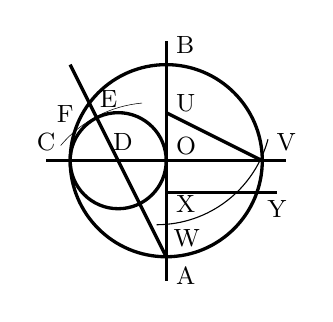
\begin{tikzpicture} [scale = 0.61]
\coordinate [label=right:\small{A}] (A) at (0, -2.4);
\coordinate [label=right:\small{B}] (B) at (0, 2.4);
\coordinate [label=above:\small{C}] (C) at (-2.5, 0);
\coordinate [label=above:\small{D}] (D) at (-0.9, 0);
\coordinate [label=above:\small{E}] (E) at (-1.2, 0.9);
\coordinate [label=above:\small{F}] (F) at (-2.1, 0.6);
\coordinate [label=right:\small{O}] (O) at (0, 0.3);
\coordinate [label=right:\small{U}] (U) at (0, 1.2);
\coordinate [label=above:\small{V}] (V) at (2.5, 0);
\coordinate [label=right:\small{W}] (W) at (-0.05, -1.6);
\coordinate [label=right:\small{X}] (X) at (0, -0.9);
\coordinate [label=right:\small{Y}] (Y) at (1.9, -1);
\draw[very thick] (0, 0) circle (2); %big circle
\draw[very thick] (-1, 0) circle (1); %small circle
\draw[thin] (-0.2, -4/3) arc (270:345:2.4); %WV
\draw[very thin] (-0.5, 1.2) arc (95:140:2.5); %FE
\draw[very thick] (-2.5, 0) -- (2.5, 0); %CV line
\draw[very thick] (0, -2.5) -- (0, 2.5); %AB line
\draw[very thick] (0, 1) -- (2, 0); %UV line
\draw[very thick] (0, -2/3) -- (2.3, -2/3); %XY line
\draw[very thick] (0, -2) -- (-2, 2); %AE line
\end{tikzpicture}\\
\textbf{Рис.2} Правильный пятиугольник
\end{center}
\end{wrapfigure}
\noindent
$\bullet$ построить окружность с це-\linebreak
тром $O$ и радиусом 1,\newline
$\bullet$ построить диаметр $AB$, ра-\linebreak
диус $OC$ перпендикулярно $AB$\linebreak
и окружность радиусом $1/2$ с\linebreak
центром в $D$ - середине $OC$,\newline
$\bullet$ прямая $AD$ делит эту окруж-\linebreak
ность в двух точках, из кото-\linebreak
рых наиболее удаленная от $A$\linebreak
точка $E$ удовлетворяет усло-\linebreak
вию: $AE=\phi(AD=\sqrt{5}/2)$ и\linebreak
$DE=1/2)$.\newline
Тогда достаточно постро-\linebreak
ить на окружности радиуса 1
с центром $O$ точку $F$ такую, что $AF=\phi$, и получаем прямоугольный
треугольник, в котором угол $(\widehat{FAB})$ равен $\pi/5$.\newline
\hspace*{15pt}Соответствующий центральный угол$(\widehat{FOB})$ равен $2\pi/5$ и позволяет\linebreak
построить правильный пятиугольник (Слейе-Мишо[48]).\newline
Существуют и другие решения, и вот одно из них, особенно про-\linebreak
стое: если $z$ есть корень 5-й степени из единицы, соотношение $z^4+$\linebreak
$z^3+z^2+z+1=0$ приводит к тригонометрическому уравнению\linebreak
$2cos\dfrac{2\pi}{5}+2cos\dfrac{4\pi}{5}+1=0$, которое просто решается, давая $cos\dfrac{2\pi}{5}=\dfrac{\sqrt{5}-1}{4}$.\linebreak
Сразу осуществимо построение. Если $U$ — середина $OB$, строим точ-\linebreak
ку $W$ , расположенную на радиусе $OA$ и удовлетворяющую равенству\linebreak
$UW=UV=\sqrt{5}/2$. Точка $X$ , середина $OW$, есть ортогональная проек-\linebreak
ция точки $Y$ такой, что угол $(\widehat{AOY})$ равен $2\pi/5$.
\noindent\textbf{8. <<Двоичное>> деление нацело}
\hspace*{15pt}\textbf{a.} Вот евклидово деление $a$ на $2b$: $a=2b\times q+r$, с $0\leqslant r<2b$. Если\linebreak
$r<b$, то евклидово деление $a$ на $b$ получается сразу: $a=b\times 2q+r$. Зато,\linebreak
если $b\leqslant r<2b$, деление таково: $a=b\times(2q+1)+(r-b)$.
\newpage


%                                  128
\textbf{b.} Предельный случай евклидова деления появляется, когда дели-\linebreak
тель больше делимого. Вот рекурсивный алгоритм вычисления частно-\linebreak
го и остатка, представленный в форме функции $Divide$:
\begin{lstlisting}[frame=single, mathescape=true]
if ($b$ > $a$)  return $(0,a)$;
else {
  $(q,r) \longleftarrow$ Divide $(a,2b)$;
  if ($r$ < $b$)  return $(2q,r)$;
  else  return $(2q+1,r-b)$; }
\end{lstlisting}
\hspace*{15pt}\textbf{d.} Недостаток рекурсивного алгоритма следующий: в ходе счета\linebreak
второй параметр функции $Divide$, который удваивается при каждом\linebreak
вызове, может превзойти первоначальные величины переменных $a$ и $b$.\linebreak
Это означает, что хотя данные и результат деления поддаются коди-\linebreak
рованию, может случиться, что в какой-либо частной реализации вели-\linebreak
чины приведут к переполнению.\newline
\hspace*{15pt}Например, когда применяют рекурсивный алгоритм к целым чи-\linebreak
слам 31001 и 15, наблюдается ряд рекурсивных вызовов, последний из\linebreak
которых — \textit{Divide}(31001,61440); если целый тип, который используют,\linebreak
записан и закодирован 16 битами, возникает переполнение, тогда как\linebreak
можно очень хорошо вычислить результат (2066,11), если остановить\linebreak
удвоение $b$ перед последней итерацией.\newline
\begin{center}
\begin{tabular}{|l|l|}
\hline
\hspace*{28pt}\underline{\textbf{A.} С переполнением}
&
\hspace*{23pt}\underline{\textbf{B.} Без переполнения}\\
{\begin{lstlisting}[mathescape=true, frame=none]
$k\longleftarrow0$;
if $b$ > $a$  return (0,$a$);
while ($b\leqslant a/2$) {
  $b\longleftarrow 2\times b$; $k\longleftarrow k+1$;
}
$q\longleftarrow 0$; $r\longleftarrow a$;
for (int $i$=1; $i\leqslant k+1$; ++$i$) {
  $q\longleftarrow 2\times q$;
  if ($r\geqslant b$) {
    $q\longleftarrow q+1$; $r\longleftarrow r-b$;
  }
  $b\longleftarrow b/2$;
}
return (q,r);
\end{lstlisting}}
&
{\begin{lstlisting}[mathescape=true, frame=none]
$k\longleftarrow 0$;
while ($b\leqslant a$) {
  $b\longleftarrow 2\times b$; $k\longleftarrow k+1$;
}
$q\longleftarrow 0$; $r\longleftarrow a$;
for (int $i=1$; $i\leqslant k$; ++$i$) {
  $b\longleftarrow b/2$; $q\longleftarrow 2\times q$;
  if ($r\geqslant b$) {
    $q\longleftarrow q+1$; $r\longleftarrow r-b$;
  }
}
\end{lstlisting}}\\
\hline
\end{tabular}
\end{center}
\begin{center}
\textbf{Алгоритм 8.} Бинарные деления
\end{center}
\newpage

%                                  129                            
Теперь уже можно — это пригодится в дальнейшем — написать\linebreak
итерационный алгоритм (8-А), который есть не что иное, как разви-\linebreak
тие предыдущего рекурсивного алгоритма ($q$ и $r$ образуют результат\linebreak
алгоритма: частное и остаток от деления). Этот алгоритм яснее вы-\linebreak
являет поставленную задачу.\\\\
\hspace*{15pt}\textbf{e.} Чтобы показать эквивалентность двух алгоритмов, можно на-\linebreak
чать с доказательства очень простого свойства: $[a/2]<b\Leftrightarrow a<2b$.\newline
\hspace*{15pt}На выходе из цикла первого алгоритма имеем свойство\linebreak
$b/2\leqslant a<b=b_02^k$ с $k>0$ - не забудем, что тело цикла использу-\linebreak
ется, по крайней мере, один раз.\newline
\hspace*{15pt}Что касается второго алгоритма, если цикл использовался, по край-\linebreak
ней мере, один раз, имеем свойство $b/2\leqslant a/2<b=b_02^k$ для $k>1$ и\linebreak
$b$ - четного. После выполнения последних присваиваний обнаруживаем\linebreak
то же свойство, что и для первого алгоритма. Если цикл не выполнен,\linebreak
это означает, что $a/2<b_0\leqslant a$, и после исполнения последних команд\linebreak
получаем $b_0=b/2\leqslant a<b=2b_0$.\newline
\hspace*{15pt}Последний алгоритм (8-В) получен, исходя из первой итерационной\linebreak
версии (8-А) извлечением из первого цикла итерации и ее слиянием с\linebreak
итерацией, взятой из второго цикла (для этого алгоритма, как и для\linebreak
предыдущего, результат - частное и остаток - представлен послед-\linebreak
ними значениями переменных $q$ и $r$).\\

\noindent\textbf{9. Построение прямых линий методами DDA}\\

\hspace*{15pt}\textbf{a.} Если $u$ и $v$ не взаимно простые числа, отрезок $[0, (u,v)]$ - не что\linebreak
иное, как повторение $d=$НОД$(u,v)$ сегментов, идентичных сегменту\linebreak
$[0,(u/d,v/d)]$.
\begin{center}
\begin{tabular}{|l|l|}
\hline
\hspace*{50pt}Алгоритм&
\hspace{5pt}Построение\\
{\begin{lstlisting}[mathescape=true, frame=none]
$y\longleftarrow 0$; $d\longleftarrow 0$; $Plot(0,0)$;
for (int $x=1$; $x\leqslant u$; ++$x$) {
  $2(vx-uy)=dc-u\leqslant d<u$.
  $d\longleftarrow d+2v$;
  if ($d\geqslant u$) {
    $y\longleftarrow y+1$; $d\longleftarrow d-2u$;
  }
  $Plot(x,y)$;
}
\end{lstlisting}}
&
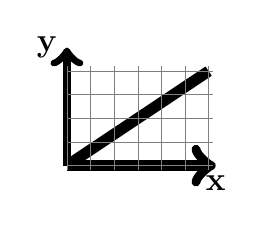
\begin{tikzpicture} [scale=0.3]
\coordinate [label=below:\textbf{\large{x}}] (x) at (6.3, 0);
\coordinate [label=left:\textbf{\large{y}}] (y) at (0, 5);
\draw[->, line width=3pt] (0, 0) to (y);
\draw[->, line width=4pt] (0, 0) to (x);
\draw[line width=4pt] (0, 0) -- (6, 4);
\draw[help lines] (0,-0.2) grid (6.2,4.2);<br>
\end{tikzpicture}\\
\hline
\end{tabular}
\end{center}
\begin{center}
\textbf{Рис. 3.} Построение прямой в первом октанте
\end{center}
\newpage


%                                  130
\textbf{b.} Выбрать для $y$ наилучшую целую аппроксимацию величины $vx/u$\linebreak
- это значит убедиться, что $|vx/u-y|\leqslant 1/2$, или еще, что\linebreak
$-u\leqslant2(vx-uy)<u$. Эта формула является в действительности ин-\linebreak
вариантом алгоритма. Поскольку нужная прямая имеет тангенс угла\linebreak
наклона меньше 1, есть только один зажигающийся пиксел на данной\linebreak
вертикали (т.е. $х$ возрастает при каждой итерации). Этот алгоритм\linebreak
(рис. 3) избегает, следовательно, пересечений маленьких горизонталь-\linebreak
ных сегментов, что дает красивый результат, когда нужны тонкие ли-\linebreak
нии; было бы совсем по-другому, если нужно <<жирное>> построение.\newline
\hspace*{15pt}Кроме того, если желаем построить этим способом прямую с накло-\linebreak
ном, большим 1, нужен второй алгоритм, идентичный первому с точ-\linebreak
ностью до перемены ролями $x$ и $y$. Наконец, построение вертикальных,\linebreak
горизонтальных или диагональных линий может проводиться наивным\linebreak
способом, который будет всегда более быстрым, чем указанный.\newline
\begin{center}
\begin{tabular}{|l|l|}
\hline
\hspace*{50pt}Алгоритм&
\hspace{5pt}Построение\\
{\begin{lstlisting}[mathescape=true, frame=none]
$x\longleftarrow 0$; $y\longleftarrow 0$; $d\longleftarrow v-u$;
for (;;) {
  $Plot(x,y)$
  $d=\delta(x,y+v-u c |\delta(x,y)|\leqslant u+v)$.
  if ($d>0$) {
    $y\longleftarrow y+1$; $d\longleftarrow d-2u$;
  } else {
    $x\longleftarrow x+1$; $d\longleftarrow d+2v$;
  }
  if (($x$==$u$) && ($y$==$v$))  break;
}
$Plot(x,y)$;
\end{lstlisting}}
&
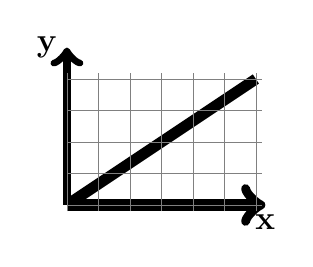
\begin{tikzpicture}[scale=0.4]
\coordinate [label=below:\textbf{\large{x}}] (x) at (6.3, 0);
\coordinate [label=left:\textbf{\large{y}}] (y) at (0, 5);
\draw[->, line width=3pt] (0, 0) to (y);
\draw[->, line width=4pt] (0, 0) to (x);
\draw[line width=4pt] (0, 0) -- (6, 4);
\draw[help lines] (0,-0.2) grid (6.2,4.2);<br>
\end{tikzpicture}\\
\hline
\end{tabular}
\end{center}
\begin{center}
\textbf{Рис. 4.} Построение прямой в первой четверти
\end{center}
\hspace*{15pt}\textbf{c.} Парадоксально, но этот алгоритм (рис. 4) - который может\linebreak
дать менее элегантные результаты, чем предыдущий, - оказывается\linebreak
немного более сложным для реализации. Действительно, нельзя больше\linebreak
предполагать, что координата $x$ возрастает после включения точки; на\linebreak
самом деле, каждая координата является \textit{доминантой} в полуквадран-\linebreak
те, о котором рассуждаем. Если рассмотреть четыре точки квадрата,\linebreak
сразу замечаем, что невозможно требовать - если не разрешены диаго-\linebreak
нальные перемещения - чтобы вертикальное расстояние правой точки\linebreak
было меньше $1/2$. Если поддерживать включенную точку в полосе фи-\linebreak
гуры 1, это влечет, между прочим, что одно из расстояний справа, го-\linebreak
\newpage


%                                  131
\noindent
ризонтальное или вертикальное, может быть сохранено меньшим 1, это\linebreak
означает, что величина $|vx-uy|$ меньше, чем $u$ или $v$. Сказать, что точ-\linebreak
ка расположена в полосе, очень точно означает, что $|2(vx-uy)|\leqslant u+v$;\linebreak
теперь покажем, что можно подтвердить это положение.\newline
\hspace*{15pt}Движение, осуществляемое на экране, будет определяться величи-\linebreak
ной $\delta(x,y)=2(vx-uy)$, получаемой после этого движения. Возможны\linebreak
два (не исключительных) случая: увеличивают $x$, величина становится\linebreak
равной $\delta(x+1,y)=\delta(x,y)+2v$, и нужно убедиться, что она остается\linebreak
меньше $u+v$, т.е. что $\delta(x,y)\leqslant u-v$. Аналогичным образом можно\linebreak
увеличить $y$, только если $u-v\leqslant\delta(x,y)$. Видим, что положение $\delta(x,y)$\linebreak
по отношению к $u-v$ определяет осуществляемые перемещения.\newline
\hspace*{15pt}Доказательство сходимости состоит в выявлении, что во время ите-\linebreak
раций $x\leqslant u$ и $y\leqslant v$. Чтобы проверить это, зная, что $x$ или $y$ растут\linebreak
при каждой итерации, можно предположить, что $x=u$ и $y<v$. В\linebreak
этих условиях оценим величину $d$: $d\geqslant\delta(u,v-1)+v-u=u+v>0$.\linebreak
Как следствие, очередная итерация увеличит $y$, и так будет до тех пор,\linebreak
пока $y<v$.\newline
\hspace*{15pt}Заметим, что по этому алгоритму построенные две вещественные\linebreak
прямые, симметричные относительно первой диагонали, не симметрич-\linebreak
ны относительно этой же диагонали (тест, применяемый к $d$, не экви-\linebreak
валентен для $x$ и $y$).\\

\noindent\textbf{10. Построение окружности методами DDA}\\

\hspace*{15pt}\textbf{a.} Функция $f$ убывает на итервале $x\in[0,R\sqrt{2}/2]$, и ее производная\linebreak
здесь меньше 1. Как следствие, $0\leqslant f(x)-f(x+1)\leqslant1$, значит, учитывая\linebreak
это, можно ограничиться уменьшением $y$ только на шаг, равный 1.\newline
\hspace*{15pt}\textbf{b.} Исходим из сделанного предположения, что $y-1$ есть луч-\linebreak
шее приближение f(x+1) тогда и только тогда, когда $y-3/2\leqslant$\linebreak
$f(x+1)<y-1/2$, т.е. $f(x+1)<y-1/2$; второе неравенство выте-\linebreak
кает из предположений по поводу f(x) и результата вопроса $a$.\newline
\hspace*{15pt}Следовательно, оцениваем на каждой итерации величину\linebreak
$e(x,y)=4y^2-4R^2-4y+4x^2+8x+5$, и нетрудно доказать, что\linebreak
$y-1/2>\sqrt{R^2-(x+1)^2}$ тогда и только тогда, когда $e(x,y)>0$, и\linebreak
еще, поскольку оперируем целыми величинами, тогда и только тогда,\linebreak
когда $d(x,y)=e(x,y)-1\geqslant 0$. Кроме того, $e(x+1,y)=e(x,y)+8x+12$\linebreak
и $e(x+1,y-1)=e(x,y)+8(x-y)+20$ и, конечно, $e(0,R)=4-4R$.\newpage



%                                  132
\begin{multicols}{2}
\begin{center}
Алгоритм
\end{center}
{\begin{lstlisting}[xleftmargin=15pt, mathescape=true]
$y\longleftarrow R$; $x\longleftarrow 0$; $s\longleftarrow 1-R$;
while (x<y) { $s=s(x,y)$
  $Plot(x,y)$;
  if ($s\geqslant 0$) {
    $s\longleftarrow s+2(x-y)+5$;
    $y\longleftarrow y-1$;
  } else {
    $s\longleftarrow s+2x+3$;
  }
  $x\longleftarrow x+1$;
}
if ($x$==$y$)  $Plot(x,y)$;
\end{lstlisting}}
\columnbreak
\begin{center}
Построение $R=14$
\end{center}
\begin{center}
\begin{tikzpicture} [scale=0.6]
\draw[->, line width=4pt] (0, -4.5) to (y);
\draw[->, line width=4pt] (-4.5, 0) to (x);
\draw[line width=3pt] (0,0) circle (4);
\draw[help lines] (-0.5,-0.5) grid (4.2, 4.2);<br>
\end{tikzpicture}
\end{center}
\end{multicols}
\begin{center}
\textbf{Рис. 5.} Построение окружности методом DDA
\end{center}
\hspace*{15pt} Рассмотрим теперь более пристально последовательность величин\linebreak
$e_i=d(x_i,y_i)-1$. Имеем следующие рекуррентные определения:
\begin{center}
\hspace*{15pt}$x_0=0$,\hspace{15pt}$y_0=R$,\hspace{15pt}$e_0=4-4R$,\newline
$x_{i+1}=x_i$,\hspace{15pt}
$y_{i+1}=\left\{ 
      \begin{gathered}
        \hspace{-53pt}y_i-1, \text{ если $e_i\geqslant0,$} \\
        y_i\text{\hspace{25pt}в противном случае,} \\ 
      \end{gathered} 
\right.$\newline
$e_{i+1}=\left\{ 
      \begin{gathered}
        \hspace{-53pt}e_i+8(x_{i+1}-y_{i+1})+20, \text{ если $e_i\geqslant0,$} \\
        e_i+8x_{i+1}+12\text{\hspace{45pt}в противном случае.} \\ 
      \end{gathered} 
\right.$
\end{center}
Значит, совершенно ясно, что эти соотношения могут упроститься (по­-\linebreak
скольку только последовательности $(х_i)$  и $(у_i)$ нас интересуют, и их\linebreak
определение зависит от знака $(e_i)$) следующим образом:
\begin{center}
\hspace*{15pt}$x_0=0$,\hspace{15pt}$y_0=R$,\hspace{15pt}$e_0=1-R$,\newline
$x_{i+1}=x_i$,\hspace{15pt}
$y_{i+1}=\left\{ 
      \begin{gathered}
        \hspace{-53pt}y_i-1, \text{ если $s_i\geqslant0$,} \\
        y_i\text{\hspace{25pt}в противном случае,} \\ 
      \end{gathered} 
\right.$\newline
$s_{i+1}=\left\{ 
      \begin{gathered}
        \hspace{-53pt}s_i+2(x_{i+1}-y_{i+1})+5, \text{ если $e_i\geqslant0,$} \\
        s_i+2x_{i+1}+3\text{\hspace{46pt}в противном случае.} \\ 
      \end{gathered} 
\right.$
\end{center}
Это соотношения, используемые в алгоритме 5.\newline
\hspace*{15pt}Когда работа алгоритма заканчивается, $x\geqslant y$, и не обязательно за­-\linebreak
жигать точку $(x,y)$. Действительно, если $x>y$, правила, которые при-\linebreak
менялись в верхнем октанте, больше недействительны (точка $(x,y)$ -\linebreak
в нижнем октанте). Зато, если $x=y$, зажигать точку нужно.\newpage


%                                  133
\textbf{c.} Аргумент Бреэенхама просто выражает тот факт, что если да­-\linebreak
на точка $(x,y)$ дискретной окружности и $|(x+1)^2+(y-1)^2-R^2|\leqslant$\linebreak
$\leqslant|(x+1)^2+y^2-R^2|$, то $|\sqrt{(x+1)^2+(y-1)^2}-R|\leqslant|\sqrt{(x+1)^2+y^2}-R|$\linebreak
(эта импликация верна также, если обратить знаки неравенств), и в\linebreak
этом случае будем брать $(x+1,y-1)$ как ближайшую точку дискретной\linebreak
окружности; в противном случае ближайшей точкой будет $(x+1,y)$.\newline
\hspace*{15pt}Обозначим $d(x,y)$ величину (положительную или отрицательную)\linebreak
$x^2+y^2-R^2$. Ясно, что $d(x+1,y)>d(x+1,y-1)$. Как следствие, знак\linebreak
суммы $s(x,y)=d(x+1,y)+d(x+1,y-1)$ указывает, какова лучшая\linebreak
(в смысле, определенном условием задачи) точка, аппроксимирующая\linebreak
окружность в этой окрестности: если $s(x,y)\geqslant$, то $P_2$ является этой\linebreak
точкой, в противном случае - это $P_1$. Из этого непосредственно выте­-\linebreak
кает алгоритм, и он соответствует эквивалентной версии алгоритма,\linebreak
построенного в вопросе \textbf{b}: достаточно положить
\begin{center}
$s_{\text{Брезенхам}}=2s_{\text{вопрос \bf{b}}}$.
\end{center}

\noindent\textbf{11. Сложность возведения в степень}\\

\hspace*{15pt}Можно сразу заметить, что $P_i$ есть степень $x$:$ P_i=x^{\alpha_i}$, кроме того,\linebreak
очевидно, что последовательность $(\alpha_i)_{\alpha_i\geqslant 0}$ является \textit{почти} цепочкой\linebreak
сложений для $n$: действительно, нет строгого возрастания $\alpha_i$, и цепь\linebreak
не обязательно начинается с 1; если исключить 1 из возможных зна­-\linebreak
чений $y_i$ и $z_i$, получили бы настоящую цепочку сложений. Как бы то\linebreak
ни было, легко видеть, что $\alpha_1\leqslant2$, $\alpha_2\leqslant 4$, $\alpha_3\leqslant8$ и т.д. Как след­-\linebreak
ствие, $\alpha_t=n\leqslant2^t$, а это доказывает, что $t\geqslant log_2n$. Это доказывает\linebreak
также, что невозможно сделать гораздо лучше, чем это делает дихото­-\linebreak
мический алгоритм возведения в степень, если разрешаются только пе-\linebreak
ремножения; точнее, можно было бы получить улучшенные результаты\linebreak
с оптимизированными цепочками сложений, но от этого не изменится\linebreak
порядок величины сложности.\\

\noindent\textbf{12. Последовательность Фибоначчи и золотое сечение}\\

\hspace*{15pt}\textbf{a.} Запишем равенства:\newline
\hspace*{80pt}$F=F_0+F_1X+F_2X^2+F_3X^3+F_4X^4+...$ ,\newline
\hspace*{71pt}$XF=$\hspace{26pt}$F_0X+F_1X^2+F_2X^3+F_3X^4+...$ ,\newline
\hspace*{67pt}$X^2F=$\hspace{58pt}$F_0X^2+F_1X^3+F_2X^4+...$ ,\\\\\\
которые непосредственно (используя определение последовательности\linebreak
Фибоначчи) подтверждают, что $F-XF-X^2F=X$. Формальный ряд\linebreak
\newpage


%                                  134
\noindent
$1-X-X^2$, будучи обратимым (так как его постоянный член - нену-\linebreak
левой), позволяет отсюда вывести, что $F=\dfrac{X}{(1-X-X^2)}$. Остается только\linebreak
разложить эту последнюю рациональную дробь на простые слагаемые.\linebreak
Нулями многочлена $X^2+X-1$ являются $-\phi$ и $-\hat{\phi}$, и быстро получается\linebreak
разложение:
\begin{center}
$F=\dfrac{-\phi}{\sqrt{5}}\times\dfrac{1}{X+\phi}+\dfrac{\hat{\phi}}{\sqrt{5}}\times\dfrac{1}{X+\hat{\phi}} = \dfrac{1}{\sqrt{5}}\left(\dfrac{-1}{1-\hat{\phi}X}+\dfrac{1}{1-\phi X}\right)$,
\end{center}
с учетом того факта, что $\phi\hat{\phi} = -1$. Еще раз беря разложения ря-\linebreak
дов, которые появляются в этом последнем выражении, выводим, что\linebreak
$F_{n}=\dfrac{1}{\sqrt{5}}(\phi^n-\hat{\phi}^n)$.\newline
\hspace*{15pt}\textbf{b.} $\phi^n+\hat{\phi}^n$ является общим членом ряда
\begin{center}
$\dfrac{1}{1-\phi X}+\dfrac{1}{1-\hat{\phi}X}=\dfrac{2-X}{1-X-X^2}=\dfrac{2F}{X}-F$.
\end{center}
Значит, $\dfrac{1}{1-X-X^2}=\dfrac{F}{X}$ является порождающим рядом последовательно-\linebreak
сти $(F_{n+1})$, следовательно, $\phi^n+\hat{\phi}^n=2F_{n+1}-F_{n}$.\newline
\hspace*{15pt}\textbf{c.} $\phi^n$ есть общий член ряда
\begin{center}
$\dfrac{1}{1-\phi X}=\dfrac{1-\hat{\phi} X}{1-X-X^2}=\dfrac{F}{X}-\hat{\phi}F$.
\end{center}

Но $\phi\hat{\phi}=-1$, и тогда, умножая на $\phi$ равенство $\phi^n=F_{n+1}-\hat{\phi}F_{n}$, получаем\linebreak
$\phi^{n+1}=\phi F_{n+1}+F_{n}$.\\

\noindent\textbf{13. Соотношения в последовательности Фибоначчи}\\

\hspace*{15pt}\textbf{a.} Нетрудно установить, что характеристическим многочленом для\linebreak
$A$ является $X^2-X-1=(X-\phi)(x-\hat{\phi})$. Матрица $A$ тогда приводится к\linebreak
диагональному виду, и легко находим базис, образуемый собственными\linebreak
векторами$(\phi,1)$ и $(\hat{\phi},1)$. Следовательно,
\begin{center}
$A^n=\dfrac{1}{\sqrt{5}}\begin{pmatrix} \phi & \hat{\phi} \\ 1 & 1 \end{pmatrix}\begin{pmatrix} \phi^n & 0 \\ 0 & \hat{\phi}^n \end{pmatrix} \begin{pmatrix} 1 & -\hat{\phi} \\ -1 & \phi \end{pmatrix} = \begin{pmatrix} F_{n+1} & F_{n} \\ F_{n} & F_{n-1} \end{pmatrix}$.
\end{center}
Конечно, простое рассмотрение первых величин $A^n$, вытекающих из\linebreak
рекуррентности, привело бы к тому же результату, но не будем отка-\linebreak
зывать себе в маленьком удовольствии (обратиться к упражнению 14\linebreak
для более общей точки зрения).
\newpage


%                                  135
Требуемые соотношения получаются соответственно вычислением\linebreak
определителя матрицы $A^n$ и использованием равенства $A^{n+m}=A^n A^m$.\linebreak
Эти соотношения обнаруживаются вновь в еще более общей форме в\linebreak
упражнениях главы II, относящимся к непрерывным дробям.\newline
\hspace*{15pt}\textbf{b.} Общий член произведения двух формальных рядов является\linebreak
сверткой $n$ первых членов каждого ряда: $\sum_{i \leqslant n}a_ib_{n-i}$. Для задачи, ко-\linebreak
торой мы занимаемся, имеем: порождающий ряд последовательности\linebreak
$f_n$ есть $F^2$ ($F$ - порождающий ряд последовательности Фибоначчи).\\\\
$F^2=\dfrac{1}{5}\left(\dfrac{1}{(1-\phi X)^2}-\dfrac{2}{(1-\phi X)(1-\hat{\phi} X)}+\dfrac{1}{(1-\hat{\phi} X)^2}\right)$\newline
\hspace*{15pt}$=\dfrac{1}{5}\left(\sum(n+1)\phi^nX^n-2(\sum\phi^nX^n)(\sum\hat{\phi}^nX^n)+\sum(n+1)\hat{\phi}^nX^n\right)$\\\\
\hspace*{15pt}$=\dfrac{1}{5}\left(\sum(n+1)(\phi^n+\hat{\phi}^n)X^n-2\sum(\sum\phi^i\hat{\phi}^{n-i})X^n\right)$.\\\\
Но мы знаем $\phi^n+\hat{\phi}^n$ (упражнение 12), и общий член второго ряда есть\linebreak
$\dfrac{\phi^{n+1}-\hat{\phi}^{n+1}}{\phi-\hat{\phi}}=F_{n+1}$. Значит,
\begin{center}
$F^2=\dfrac{1}{5}\left(\sum(n+1)(2F_{n+1}-F_n)X^n-2\sum F_{n+1}X^n\right)$
\end{center}
\begin{center}
или\hspace{15pt}$\displaystyle\sum_{k=0}^nF_kF_{n-k} = \dfrac{2nF_{n+1}-(n+1)F_n}{5}$.
\end{center}

\noindent\textbf{14. Линейные рекуррентные последовательности $k$-го\newline
порядка}\\

\hspace*{15pt}\textbf{a.} Действуем, выполняя преобразования над порождающими ряда-\linebreak
ми. Пусть $\mathcal{F}$ - порождающий ряд последовательности. Как для по-\linebreak
следовательности Фибоначчи, можно легко установить, что $(1-X-$\linebreak
$X^2)\mathcal{F}=x_0+X(x_1-x_0)$. Следовательно,
\begin{center}
$\mathcal{F}=\dfrac{x_0+X(x_1-x_0}{1-X-X^2}=x_0\dfrac{F}{X}+(x_1-x_0)F$.
\end{center}
Значит, $x_n=x_0F_{n+1}+(x_1-x_0)F_n=x_1F_n+x_0F_{n-1}$.\\\\
\hspace*{15pt}\textbf{b.} Ясно, что множество рассмотренных последовательностей явля-\linebreak
ется векторным пространством размерности $k$, и существует изомор-\linebreak
физм между этим пространством и $K^k$: он ставит в соответствие ка-\linebreak
\newpage



%                                  136
\noindent
ждой последовательности ее $k$ первых членов. Полным прообразом ка-\linebreak
нонического базиса $K^k$ является то, что называется фундаменталь-\linebreak
ным базисом пространства последовательностей. Обозначим этот базис\linebreak
$(x^{k-1},...,x^0)$ ($x^0$ есть полный прообраз вектора $(0,...,0,1))$. Матрица\linebreak
$A$, которая действует в $K^k$, соответствует при этом изоморфизме опе-\linebreak
ратору сдвига последовательностей. Тогда столбцы матрицы $A$ суть\linebreak
выборки $(x_k^i,...,x_1^i)$ из последовательностей $x^i$. Это означает еще, что\linebreak
\begin{center}
$A^n=\begin{pmatrix}
x_{n+k-1}^0 & x_{n+k-1}^1 & \cdots & x_{n+k-1}^{k-1} \\
x_{n+k-2}^0 & x_{n+k-2}^1 & \cdots & x_{n+k-2}^{k-1} \\         
\vdots & \vdots & \ddots & \vdots \\
x_n^0 & x_n^1 & \cdots & x_n^{k-1}
\end{pmatrix}$.
\end{center}
В случае, когда $k=2$, фундаментальный базис пространства последова-\linebreak
тельностей образован последовательностью Фибоначчи и ее \textit{сдвигами}.\linebreak
Тут же обнаруживается результат предыдущего вопроса и матричное\linebreak
равенство упражнения 13.\\

\noindent\textbf{15. Дихотомия по Горнеру}\\

\hspace*{15pt}\textbf{a.} Конечно, $P_0=P$ и $P_k=a_k$. Соотношение между $P_i$ и $P_{i-1}$,\linebreak
которое определяет метод Горнера, есть $P_{i-1}=X P_i+a_{i-1}$.\newline
\hspace*{15pt}\textbf{b.} Если предположить, что $n=\sum b_i2^i$, то можно рассмотреть мно-\linebreak
гочлен $P=\sum b_iX^i$ и вычислить элементы $x^{P_i(2)}$, используя предыдущее\linebreak
рекуррентное соотношение. Это дает алгоритм:
\begin{lstlisting}[xleftmargin=15pt, mathescape=true]
$R\longleftarrow 1$;
for (int $i=n$; $i\geqslant 0$; --$i$) {
  $R\longleftarrow R^2\times x^{b_i}$; $R=x^{b_n2^{n-i}+b_{n-1}2^{n-i-1}+...+b_i}=x^{P_i(2)}$
}
return $R$;
\end{lstlisting}
Этот алгоритм может быть оптимизирован исключением ненужных\linebreak
перемножений следующим образом:
\begin{lstlisting}[xleftmargin=15pt, mathescape=true]
$R\longleftarrow 1$;
for (int $i=n$; $i\geqslant 0$; --$i$) {
  $R\longleftarrow R^2$;
  if ($b_i$==$1$)  $R\longleftarrow R\times x^{b_i}$;
  $R=x^{b_n2^{n-i}+b_{n-1}2^{n-i-1}+...+b_i}=x^{P_i(2)}$
}
return $R$;
\end{lstlisting}


%                                  137
\textbf{c.} Если неизвестно двоичное разложение $n$, то ясно, что нужно бу-\linebreak
дет тем или иным способом вычислить его более или менее неявно по\linebreak
ходу выполнения алгоритма. Если известно, что $2^k \leqslant n < 2^{k+1}$, то это\linebreak
влечет, что двоичный разряд порядка $k$ числа $n$ равен 1, что позво-\linebreak
ляет запустить счет. Затем достаточно определить, принадлежит ли\linebreak
$n-2^k$ интервалу $[a^{k-1},2^k]$, чтобы узнать величину двоичного разряда\linebreak
порядка $k-1$. Все это приводит к следующему алгоритму (который не\linebreak
касается случая $n=0$):
\begin{lstlisting}[xleftmargin=15pt, mathescape=true]
$\alpha\longleftarrow 1$;
while ($\alpha\leqslant n-\alpha$)  $\alpha\longleftarrow 2\alpha$;
Ici $2\alpha>n\geqslant \alpha=2^k$
$R\longleftarrow x$; $m\longleftarrow n-\alpha$;
for (;;) {
  $x^n=R^\alpha x^m$ et $0\leqslant m<\alpha$, $\alpha$ est une puissance de 2
  if ($\alpha==1$)  break;
  $\alpha\longleftarrow \alpha/2$; $R\longleftarrow R^2$;
  if ($m\geqslant \alpha$) {
    $R\longleftarrow R\times x$;
    $m\longleftarrow m-\alpha$;
  }}
return $R$;
\end{lstlisting}
\hspace*{15pt}В этом алгоритме все начинается с определения $\alpha=2^k$ такого, что\linebreak
$a^k \leqslant n < 2^{k+1}$ (только без того, чтобы результаты промежуточных\linebreak
вычислений превосходили $n$), затем продолжается вычисление $x^n$.\newline
\hspace*{15pt}\textbf{d.} В этом случае, когда сложность одного перемножения постоянна\linebreak
(независимо от размеров сомножителей), устанавливаем, что имеется\linebreak
самое большее $k$ итераций, каждая из которых содержит 1 или 2 умно-\linebreak
жения; следовательно, сложность оценивается сверху числом $2log_2n$.\newline
\hspace*{15pt}В случае, когда сложность элементарного умножения не постоянна,\linebreak результат совершенно другой.\\

\noindent\textbf{16. Вычисление чисел Фибоначчи}\\

\hspace*{15pt}\textbf{a.} Несложно написать рекурсивный аглоритм, подобный следующе-\linebreak
му:
\begin{lstlisting}[xleftmargin=15pt, mathescape=true]
if ($n==0$)  return 0;
else if ($n==1$)  return 1;
else return $\textit{Фибоначчи}(n-1)+\textit{Фибоначчи}(n-2)$;
\end{lstlisting}
\hspace*{15pt}Число рекурсивных вызовов в действительности равно $2\sum_{i=1}^{n-1}F_i=$\linebreak
$2(F_{n+1}-1)$ (доказать этот результат), что дает экспоненциальную\linebreak
сложность.\newpage



%                                  138
Вдохновившись, напротив, методом, использованным для алгорит-\linebreak
ма Евклида, состоящим в преобразовании пар последовательных эле-\linebreak
ментов в последовательность: $(F_{n+2},F_{n+1})=(F_{n+1}+F_n,F_{n+1})$ (фор-\linebreak
мула, которая имеет связь с матрицей упражнения 14), приходим к ал-\linebreak
горитму, который для $n$ вычисляет пару чисел Фибоначчи $(F_{n+1},F_n)$:
\begin{lstlisting}[xleftmargin=15pt, mathescape=true]
if ($n==0$)  return $(1,0)$;
else {
  $(F_n,F_{n-1})\longleftarrow\textit{Фибоначчи}(n-1)$;
  return $(F_n+F_{n-1},F_n)$;
}
\end{lstlisting}
\hspace*{15pt}Этот алгоритм, который легко может быть сделан нерекурсивным,\linebreak
имеет сложность, пропорциональную $n$ (линейную, а не экспоненциаль-\linebreak
ную).\\
\hspace*{15pt}\textbf{Ь.} Любое из соотношений:\\\\
\hspace*{5pt}$F_{n-1}+\phi F_n=\phi^n$,\hspace{40pt}
$\begin{pmatrix}
F_n \\ F_{n-1}
\end{pmatrix}=
\begin{pmatrix}
1 & 1 \\ 1 & 0
\end{pmatrix}^n
\begin{pmatrix}
1 \\ 0
\end{pmatrix}$,\hspace{40pt}$F_n=\dfrac{\phi^n-\hat{\phi}^n}{\sqrt{5}}$\newline
приводит к мысли, что $F_n$ может быть вычислено методом дихотоми-\linebreak
ческого возведения в степень. Это действительно так! Обоснуем наше\linebreak
решение с помощью, например, первого соотношения (другие приво-\linebreak
дят к тому же методу). В несколько научной манере можно сказать,\linebreak
что $\phi$ принадлежит кольцу $\mathbb{Z}[\phi]$, состоящему из $a+\phi b$ с целыми $a$, $b$.\linebreak
Устойчивость относительно произведения в $\mathbb{Z}[\phi]$ вытекает из уравне-\linebreak
ния $\phi^2=\phi+1$:
\begin{center}
$(a+\phi b)(c+\phi d)=ac+\phi(ad+bc)+\phi^2bd=(ac+bd)+\phi(ad+b(c+d))$.
\end{center}
Эта формула показывает, к тому же, как считать в $\mathbb{Z}[\phi]$ с помощью це-\linebreak
лых операций. Следовательно, вычисление $\phi^n$ может быть осуществлено\linebreak
через дихотомию; как это видим по вышеупомянутой формуле, слож-\linebreak
ность одного перемножения в $\mathbb{Z}[\phi]$ есть 4 целых перемножения и 3 целых\linebreak
сложения, тогда как сложность возведения в квадрат — 3 целых перем-\linebreak
ножения и 2 сложения: $(a+\phi b)^2=(a^2+b^2)+\phi b(2a+b)$, что приводит\linebreak
к алгоритму 9-А.\newline
\hspace*{15pt}Но можно сделать лучше; соотношение
\begin{center}
$(a+bX)(c+dX)=ac+\left((a+b)(c+d)-ac-bd\right)X+bdX^2$
\end{center}
доказывает, что можно умножать два многочлена первой степени с по-\linebreak
мощью только 3 перемножений, но 4 сложений (об этом снова пойдет\linebreak
\newpage


%                                  139
\noindent
речь в главе V). Применительно к кольцу $\mathbb{Z}[\phi]$ оно позволяет вычислить\linebreak
произведение с помощью 3 целых перемножений и 4 целых сложений:
\begin{center}
$(a+\phi b)(c+\phi d)=ac+bd+\phi((a+b)(c+d)-ac)$,
\end{center}
и, конечно, использовались при реализации.\newline
\hspace*{15pt}\textbf{c.} Можно вычислить $\phi^n$ через дихотомию, но применяя метод\linebreak
упражнения 15 (использование метода Горнера). Заметим, что одна\linebreak
из компонент аддитивных перемножений в этом способе постоянна\linebreak
(равна элементу, степень которого хотим вычислить): здесь это умно-\linebreak
жение на $\phi$, которое не является настоящим умножением, так как\linebreak
$(a+b\phi)\phi=b+\phi(a+b)$. В алгоритме 9-В последовательные степени\linebreak
$\phi$ вычислены в паре $(g,g')$, представляющей $g+\phi g'$.
\begin{center}
\begin{tabular}{|l|l|}
\hline
\hspace*{20pt}\underline{\textbf{A.} Традиционная дихотомия}&
\hspace*{5pt}\underline{\textbf{B.} Дихотомия <<по Горнеру>>}\\
{\begin{lstlisting}[mathescape=true, frame=none]
$(f,f')\longleftarrow(1,0)$; $(g,g')\longleftarrow(0,1)$;
$i\longleftarrow n$;
for (;;) { $(f+\phi f')\times(g+\phi g')^i=\phi^n$
  if ($i\%2==1$) {
   $(f,f')\longleftarrow(fg+f'g',fg'+f'(g+g'))$;
  }
  $i\longleftarrow [i/2]$;
  $(f+\phi f')\times(g+\phi g')^{2i}=\phi^n$
  if ($i==0$)  break;
  $(g,g')\longleftarrow(g^2+g'^2,g'(2g+g'))$;
}
return $f'$; $f+\phi f'=\phi^n$
\end{lstlisting}}
&
{\begin{lstlisting}[mathescape=true, frame=none]
$n=\epsilon_q 2^q+\epsilon_{q-1}2^{q-1}+...+\epsilon_0$
$(g,g')\longleftarrow(1,0)$;
for (int $i=q$; $i\geqslant 0$; $--i$) {
  $(g,g')\longleftarrow (g^2+g'^2, g'(2g+g'))$;
  if ($\epsilon_i==1$) {
    $(g,g')\longleftarrow(g',g+g')$;
  }
}
return $g'$;
\end{lstlisting}}\\
\hline
\end{tabular}
\end{center}

\begin{center}
\textbf{Алгоритм 9.} Вычисление чисел Фибоначчи
\end{center}

\noindent\textbf{17. $\epsilon$-лексикографический порядок и знакопеременный лексикографический порядок}\\

\hspace*{15pt}\textbf{a.} $\epsilon$-лексикографический порядок является линейным, если исход-\linebreak
ные упорядочения линейны. Если функция $\epsilon$ тож дественно равна 1, по-\linebreak
лучаем тогда обычный лексикографический порядок.
\newpage



%                                  140
\begin{wraptable}{i}{0.6\textwidth}
\centering
\begin{tabular}{|ccccc|}
\hline
$(e_1,f_4)$ & $\rightarrow$ & $(e_2,f_4)$ &  & $(e_3,f_4)$ \\
$\uparrow$ &  & $\downarrow$ &  & $\uparrow$ \\
$(e_1,f_3)$ &  & $(e_2,f_3)$ &  & $(e_3,f_3)$ \\
$\uparrow$ &  & $\downarrow$ &  & $\uparrow$ \\
$(e_1,f_2)$ &  & $(e_2,f_2)$ &  & $(e_3,f_2)$ \\
$\uparrow$ &  & $\downarrow$ &  & $\uparrow$ \\
$(e_1,f_1)$ &  & $(e_2,f_1)$ & $\rightarrow$ & $(e_3,f_1)$ \\ \hline
\end{tabular}
\end{wraptable}
\textbf{b.} Эта история с планкой наводит на мысль о том, что происходит внутри $E\times F$; функция $F\ni y\longmapsto(x,y)\in$\linebreak
$\in x\times F$ является изоморфизмом, если $\epsilon(x)=1$, в противном случае антиизоморфизмом.\newline
\hspace*{15pt}\textbf{c.} Убеждаемся, что $min_{E\times F}=(min_E,min_F)$. Определение набольшего элемента немного сложнее:\newline
\hspace*{15pt}$max_{E\times F}=(max_E,min_F)$, если мощность множества $E$ - четна, и\linebreak
$max_{E\times F}=(max_E, max_F)$, если мощность множества E - нечетна.\newline
\hspace*{15pt}Проиллюстрируем это с помощью примера: пусть $E=\{e_1<e_2<e_3\}$\linebreak
и $F=\{f_1<f_2<f_3<f_4\}$; тогда знакопеременное лексикографическое\linebreak
произведение $E\times F$ представляется так, как это показано в таблице\linebreak
выше.\newline
\hspace*{15pt}Последующий элемент для $(x,y)\in E\times F$ вычисляется тогда рекур-\linebreak
сивно, например, с использованием алгоритма 10-A.
\begin{center}
\begin{tabular}{|l|l|}
\hline
\hspace*{20pt}\underline{\textbf{A.} Рекурсивная версия}&
\hspace*{5pt}\underline{\textbf{B.} Итеративная версия}\\
{\begin{lstlisting}[mathescape=true, frame=none]
if ($\epsilon(x)==1$ && $y<\text{max}_F$)
  return $(x,\text{succ}_F(y))$;
else if ($\epsilon(x)==-1$ && $y>\text{min}_F$)
  return $(x,\text{предш}_F(y))$;
else if ($x<\text{max}_E$)
  return $(\text{succ}_E(x),y)$;
else
  ici, $(x,y)=max_{E\times F}$;
\end{lstlisting}}
&
{\begin{lstlisting}[mathescape=true, frame=none]
$s\longleftarrow\text{sign}_{E_1}(x_1)\text{sign}_{E_2}(x_2)...\text{sign}_{E_n}(x_n)$;
for (int $i=n$; $i\geqslant 1$; $--i$) {
 $s\longleftarrow s\times\text{sign}_{E_i}(x_i)$;
 $s=\text{sign}_{E_1}(x_1)\text{sign}_{E_2}(x_2)...
 \text{sign}_{E_{i-1}}(x_{i-1})$
 if ($s==1$ && $x_i<\text{max}_{E_i}$) {
   $x_i\longleftarrow\text{succ}_{E_i}(x_i)$;
   return $x$;
 } else if ($s==-1$ && $x_i>\text{min}_{E_i}$) {
   $x_i\longleftarrow\text{предш}_{E_i}(x_i)$;
   return $x$;
 }
}
$x=\text{max}_E$;
return $Successor_Error$;
\end{lstlisting}}\\
\hline
\end{tabular}
\end{center}
\begin{center}
\textbf{Алгоритм 10.} Последующий элемент в знакопеременном\newline
лексикографическом порядке
\end{center}
\hspace*{15pt}В этом алгоритме замечаем, что единственная составляющая мо-\linebreak
дифицирована и заменена своим последующим или предшествующим\linebreak
элементом. Отсюда следует, что функция $\mu(x,y)=sign_E(x)\times sign_F(y)$\linebreak
со значениями из $\{1, -1\}$ является <<знакочередующейся>>, т.е. удовле-\linebreak
творяет равенству $\mu(succ(x,y))=-\mu(x,y)$. Поскольку она равна 1 на\linebreak
\newpage



%                                  141
\noindent
$min_{E\times F}=(min_E,min_F)$, то она совпадает с функцией-сигнатурой на\linebreak
$E\times F$.\newline
\hspace*{15pt}\textbf{d.} Пусть $E_1, E_2, ...,E_n - n$ конечных линейно упорядоченных\linebreak
множеств. Обозначим $sign_{E_i}$, фуцнкцию-сигнатуру на $E_i$, единственную\linebreak
функцию, отображающую $E_i$ на множество $\{-1,1\}$, удовлетворяющую\linebreak
условиям $sign_{E_i}(min_{E_i})=1$ и для $x\in E_i-\{max_{E_i}\}sign_{E_i}(succ_{E_i}(x))=$\linebreak
$-sign_{E_i}(x)$. Обозначим через $\epsilon_i:E\rightarrow\{-1,1\}$ функцию, определенную\linebreak
через $\epsilon_i(x)=\Pi_{j<i}sign_{E_j}(x_1)$. На декартовом произведении $E=E_1\times$\linebreak
$E_2\times ... \times E_n$ определим отношение $<: (x_1,...,x_n)<(y_1,...,y_n)$ тогда\linebreak
и только тогда, когда наименьшее $i$ такое, что $x_i\neq y_i$, удовлетворяет\linebreak
неравенству $x_i\leqslant^{\epsilon_i(x)}y_i$.\newline
\hspace*{15pt}Легко убедиться, что отношение <<$x=y$ или $x<y$>> является отноше-\linebreak
нием порядка на $E$, которое есть не что иное, как отношение порядка,\linebreak
изученное в предыдущем упражнении для $n=2$. Это отношение линей-\linebreak
ного порядка, наименьший элемент которого есть $min_E=(min_{E_1},...,$\linebreak
$min_{E_n})$.\newline
\hspace*{15pt}Сигнатура линейно упорядоченного множества $E$ есть  <<произведе-\linebreak
ние  сигнатур  каждой  компоненты>>; это  можно  доказать  с  помощью\linebreak
индукции, используя ассоциативность: $(E_1\times E_2)\times E_3=E_1\times(E_2\times E_3)$,\linebreak
которая вытекает из-того факта, что сигнатура произведения \textit{двух} ко-\linebreak
нечных линейно упорядоченных множеств есть произведение их сигна-\linebreak
тур.\newline
\hspace*{15pt}Следующий  вопрос  показывает,  что  последующий элемент для\linebreak 
$(x_1,...,x_n)$ получается изменением \textit{единственной компоненты} $x_i$ и ее\linebreak 
заменой своей последующей или предыдущей в $E_i$. Функция
\begin{center}
$\mu(x_1,...,x_n)=sign_{E_1}(x_1)...sign_{E_n}(x_n)$
\end{center}
для $x\neq max_E$ удовлетворяет равенству $\mu(succ_E(x))=-\mu(x)$ и, посколь-\linebreak
ку для $min_E$ она равна 1, это $-$ сигнатура множества $E=E_1\times...\times E_n$.\linebreak
\hspace*{15pt}\textbf{e.} Как и для лексикографического порядка, последующий элемент\linebreak
для $x=(x_1,...,x_n)$ получается в результате \textit{попыток} варьировать по-\linebreak
следнюю компоненту $x_n$ и ее замены на $succ_{E_n}(x)$ (если $\epsilon_n(x)=1$),\linebreak
или на предш$_{E_n}(x)$ (если $\epsilon_n(x)=-1$). Если это невозможно, т.е. если\linebreak
$\epsilon_n(x)=1$ и $x_n=max_{E_n}$, либо $\epsilon_n(x)=-1$ и $x_n=min+{E_n}$, то пробуем\linebreak
сварьировать предпоследнюю компоненту $x_{n-1}$ по аналогичному пра-\linebreak
вилу..., что приводит к окончательному алгоритму (10-B).\\

\noindent\textbf{18. Перебор делителей целого числа}\\

\hspace*{15pt}Делитель числа $n=p_1^{\alpha_1}p_2^{\alpha_2}...p_k^{\alpha_k}$ полностью определен данной по-\linebreak
следовательностью $(\beta_1,\beta_2,...,\beta_n)$, которая удовлетворяет соотношени-\linebreak
\newpage



%                                  142
\noindent
ям $0\leqslant \beta_i\leqslant \alpha_i$ для $i=1,2,...,n$. \textit{Смена} делителя $n$ сводится, значит, к\linebreak
смене показателей простых множителей. Если выбрать порядок, опре-\linebreak
деленный на показателях, т.е. на произведении $[0,\alpha_1]\times...\times[0,\alpha_n]$, и\linebreak
вычислить делитель в переменной $P$, тогда достаточно \textit{одного деле}-\linebreak
\textit{ния или умножения} для вычисления последователя для $P$. Действитель-\linebreak
но, если $P$ записывается: $P=p_1^{\beta_1}p_2^{\beta_2}...p_k^{\beta_k}$, и если $i$ является индек-\linebreak
сом компоненты, которая изменилась в вычислении последующего для\linebreak
$(\beta_1,\beta_2,...,\beta_n)$, то $succ(P)=P\times p_i$  или же $succ(P)=P/p_i$. Возьмем\linebreak
пример: $n=p^3q^3r^2$; последовательные величины для P, т.е. список де-\linebreak
лителей n, тогда получается так: $p^0q^0r^0$, $p^0q^0r^1$, $p^0q^0r^2$, $p^0q^1r^2$, $p^0q^1r^1$,\linebreak
$p^0q^1r^0$, $p^0q^2r^0$, $p^0q^2r^1$, $p^0q^2r^2$, $p^0q^3r^2$, $p^0q^3r^1$, $p^0q^3r^0$, $p^1q^3r^0$, $p^1q^3r^1$,\linebreak
...\\

\noindent\textbf{19. Код Грея}\\

\textbf{a.} Достаточно рассмотреть множество
\begin{center}
$\{0,1\}^n=\{0,1\}\times\{0,1\}\times...\times\{0,1\}$
\end{center}
и наделить его знакопеременным лексикографическим порядком. Мож­-\linebreak
но также рассуждать с помощью индукции по $n$:  если $s_1, ..., s_{2^n-1}$\linebreak
является кодом Грея для цепочек из $n$ разрядов, то:\newline
\hspace*{25pt}$(0,s_0)$,\hspace{15pt}$(0,s_1),...,(0,s_{2^n-2})$,\hspace{15pt}$(0,s_{2^n-1})$,\hspace{15pt}$(1,s_{2^n-1})$,\newline
\hspace*{250pt}$(1,s_{2^n-2}),...,(1,s_1), (1,s_0)$\newline
\hspace*{25pt}и\hspace{15pt}$(0,s_0)$,\hspace{15pt}$(1,s_0)$,\hspace{15pt}$(1,s_1)$,\hspace{15pt}$(0,s_1),...,(0,s_{2^n-2})$,\newline
\hspace*{197pt}$(1,s_{}2^n-2)$,\hspace{15pt}$(1,s_{2^n-1})$,\hspace{15pt}$(0,s_{2^n-1})$\newline
суть два кода Грея для цепочек из $n+1$ разрядов.\newline
\textbf{b.} Используя первый из только что данных примеров кода Грея,\linebreak
можно довольно просто построить требуемую программу. Для этого\linebreak
применяют две взаимно рекурсивные процедуры: одна генерирует код\linebreak
Грея, другая $-$ его зеркальное отражение. Каждая из этих двух про­-\linebreak
цедур $Gray$ и $Reverse_Gray$ обладает двумя параметрами, второй обо­-\linebreak
значает цепочку из 1 или 0, которая должна быть помещена в качестве\linebreak
приставки каждого слова кода Грея, длина которой задается первым\linebreak
параметром. Главный  вызов, который должен быть осуществлен для\linebreak
получения вывода на экран кода Грея длины $n$, есть $\blacktriangleright Gray (n) \blacktriangleleft$. Вот\linebreak
первая из этих процедур:
\newpage



%                                  143
\begin{lstlisting}[mathescape=true]
void $Gray$(int $n$, string $Prefix$) {
  if ($n==0$) $Put\_Line(Prefix)$;
  else {
    $Gray(n-1, Prefix \& "0")$; $Reverse\_Gray(n-1, Prefix \& "1")$;
  }
}
\end{lstlisting}
\hspace*{15pt}Вторая процедура $Reverse\_Gray$ получается перестановкой вхожде-\linebreak
ний цепочек "1" и "0".\newline
\hspace*{15pt}\textbf{c.} Чтобы написать итерационный алгоритм, достаточно использо­-\linebreak
вать результат упражнения 17, но факт работы с $\{0,1\}$ приносит зна-\linebreak
чительные упрощения. Изучим знакопеременное лексикографическое произведение вида $E\times\{0,1\}$, где $E-$ конечное линейно упорядочен-\linebreak
ное множество, и рассмотрим последователя для элемента $(x_1,x_2)\in$\linebreak
$E\times\{0,1\}$ \textit{в случае, когда этот последователь получается изменени-\linebreak
ем компоненты} $x_2$; это проявляется в следующих ситуациях:
\begin{multicols}{2}
\begin{lstlisting}[mathescape=true, caption=Код Грея]
$s:=x_1+x_2+...+x_n\mod{2}$;
for (int $i=n$; $i\geqslant 1$; $--i$) {
  if ($s==0$) {
    $x_i\longleftarrow 1-x_i$;
    return $x$;
  }
  $s\longleftarrow(s+x_i)\mod{2}$;
}
return $Successor_Error$;
\end{lstlisting}
\columnbreak
$\bullet (x_1,x_2)=(x_1,0)$ и $sign(x_1)=1$,\newline
значит, $succ(x_1,0)=(x_1,1)$,\newline
$\bullet (x_1,x_2)=(x_1,0)$ и $sign(x_1)=-1$,\newline
значит, $succ(x_1,1)=(x_1,0)$.\newline
Можно свести эти два случая к од-\newline
ному: $sign(x_1,x_2)=1$ и $succ(x_1,x_2)=$\linebreak
$(x_1,1-x_2)$, что приводит к алгоритму\linebreak
вычисления последователя для элемента,\linebreak
который приведен слева.
\end{multicols}
\hspace*{15pt}Несколько замечаний, однако, к этому алгоритму: прежде всего,\linebreak
вместо использования сигнатуры рассуждаем в терминах четности це-\linebreak
пи рассматриваемых разрядов; затем, нормальный выход из цикла (по\linebreak
исчерпании итераций) происходит только для последнего элемента ко-\linebreak
да, что объясняет возбуждение исключения.\\
\noindent\textbf{20. Изменение слов в обратном коде Грея}\\
\hspace*{15pt}\textbf{a.} Очевидно, что $T_1 = (1)$. С другой стороны, обратный код\linebreak
Грея таков, что если $G_n$ является таким кодом из $n$ разрядов, то\linebreak
$(0G_n,1\overline{G_n}) - $обратный код Грея из $n+1$ разрядов, запись $\overline{G_n}$ озна-\linebreak
чает обращенную последовательность $G_n$. при этих условиях $T_{n+1}=$\linebreak
$T_n\cdot(n+1)\cdot\overline{T_n}$, и тот факт, что $\overline{T_1}=T_1$, доказывает с помощью индук-\linebreak
ции требуемое свойство.\newline
\hspace*{15pt}\textbf{b.} Этот алгоритм, выведенный из тонких методов освобождения от\linebreak
рекурсивности, является искусственным, но обезоруживающе простым.
\newpage



%                                  144
Очевидно, что при $k=1$ он дает последовательность $T_1$ (сведенную к\linebreak
элементу 1). Кроме того, в этом случае выполнена единственная ите-\linebreak
рация, что влечет при выходе из цикла $Stack(1)=x$ и $Stack(2)=2$.\newline
\hspace*{15pt}Сделаем теперь индуктивное предположение, что этот алгоритм ве-\linebreak
дет себя так, как описано в условии, для
$k=n-1$. Если $k=n$, то он\linebreak
начинает \textit{создавать} последовательность $T_{n-1}$ (гипотеза индукции), и\linebreak
после этого обнаруживаем, что $Stack(1)=n$ и $Stack(n)=n$, а другие\linebreak
элементы массива стека остаются неизмененными по отношению к пер-\linebreak
воначальной конфигурации. В этой последней ситуации осуществляем\linebreak
итерацию, по ходу которой все начинается
с \textit{получения} $Stack(1)=n$,\linebreak
возвращаем $Stack(1)$ к 1, затем переносим значение $x=Stack(n+1)$\linebreak
на место $n$ и заменяем $Stack(n+1)$ на $n+1$. Тогда оказываемся в си-\linebreak
туации, которая заставляет алгоритм заново создавать последователь-\linebreak
ность $T_{n-1}$. Тут остается проверить, что на выходе из этого второго\linebreak
захода содержани массива $Stack$ согласуется с гипотезой индукции;\linebreak
принимая во внимание конфигурацию, предшествующую этому второ-\linebreak
му заходу $(Stack(n)=n+1)$ и $Stack(n+1)=n+1$, видим, что эта\linebreak
проверка является лишь формальностью.\newline
\hspace*{15pt}Запись пактеа, реализующего шаг за шагом генерацию слов ко-\linebreak
да, требует нескольких предостережений, прежде всего, нельзя боль-\linebreak
ше удовлетворяться представлением слова кода только как функции\linebreak
вычисления последущего элемента, нужно получить также таблицу\linebreak
$Stack$, вытекающую из последнего вычисления; затем, когда достигнуто\linebreak
последнее слово кода, исполнение тела цикла будет вызывать ошибку\linebreak
переполнения. Можно сгладить этот недостаток, заменяя последнюю\linebreak
инструкцию тела цикла на $Stack(1+(t\mod{n}))\longleftarrow 1+(t\mod{n})$; эта\linebreak
модификация позволяет алгоритму бесконечно создавать один и тот\linebreak
же код Грея.\newline
\hspace*{15pt}Еще можно заметить, что этот способ генерации кода Грея, благо-\linebreak
даря изменениям, которые нужно проделать, позволяет создать цикл\linebreak
в обратном коде Грея, начинающийся с какой угодно конфигурации.\linebreak
Цикл, который проходится таким образом, выводится из \textit{стандартно-}\linebreak
\textit{го} кода (того, которому выше дано рекурсивное определение) трансля-\linebreak
цией всех слов кода (трансляция означает здесь покомпонентное сложе-\linebreak
ние по модулю 2).\\

\noindent\textbf{21. Вычисление перманента матрицы}\\

\textbf{a.} Центральный член может быть рассмотрен как однородный мно-\linebreak
гочлен степени $n$ от переменных $a_{ij}$, который можно выразить суммой\linebreak
$\sum\mu_{\alpha}a_{1\alpha(1)}...a_{n\alpha(n)}$, распространяющейся на все \textbf{отображения} $\alpha$ из
\newpage



%% \begin{106/145-162}

\DeclarePairedDelimiter{\abs}{\lvert}{\rvert}
\DeclarePairedDelimiter{\floor}{\lfloor}{\rfloor}

\lhead{\small\textit{Решения упражнений}}
\rhead{145}

\noindent
[1, $n$] в [1, $n$], при этом коэффициент $\mu_\alpha$ определяется суммой

\begin{equation*}
\mu_{\alpha} = \sum_{\epsilon_i\in\{0,1\}} (-1)^{\epsilon_1+...+\epsilon_n} \epsilon_{\alpha(1)}...\epsilon_{\alpha(n)}.
\end{equation*}

\noindent
Если $\alpha$ — перестановка, коэффициент $\mu_\alpha$ равен $(—1)^n$, поскольку единственный ненулевой член суммы — это тот, для которого все $\epsilon_i$, равны 1. В противном случае можно разложить $\mu_\alpha$ следующим образом:

\begin{equation*}
\sum_{\epsilon_i, i \neq k} (-1)^{\epsilon_1+...+\epsilon_n} \sum_{\epsilon_k=0,1} (-1)^{\epsilon_k} \epsilon_{\alpha(1)}...\epsilon_{\alpha(n)},
\end{equation*}

\noindent
где $k$ — элемент из [1, $n$], который не принадлежит образу $\alpha$, и хорошо видно, что внутренний член (сумма по $\epsilon_k$) равен нулю; это доказывает, что $\mu_\alpha$ в этом случае равно нулю. Второе искомое выражение (суммы которого записываются на множествах) просто выводится из первого, исключением ненулевых $\epsilon_i$, появляющихся в сумме.

\setcounter{lstlisting}{11}
\captionsetup[lstlisting]{labelfont={bf}}

\begin{wrapfigure}{r}{7cm}
\begin{lstlisting} [language=C,
					basicstyle=\small,
					linewidth=7cm, 
					belowskip=-1em,
					mathescape=true, 
					caption=Вычисление перманента]
S[1] = a[1][succ($n$)]; P = S[1];
for (int i = 2; i <= n; ++i)
	S[i] = a[i][succ($n$)]; P *= S[i];
$\sum$ = -P; E = succ($n$);
while (E != E$_{max}$) {
	j = E $\Delta$ E$^{'}$; S[1] $\pm$= a[1][j];
	P = pow(-1, abs(E$^{'}$)) * S[1];
	for (int i = 2; i <= n; ++i)
		S[i] $\pm$= a[i][j]; P *= S[i];
	$\sum$ += P; E = E$^{'}$;
}
return pow(-1, n) * $\sum$;
\end{lstlisting}
\end{wrapfigure}

\subparagraph{b.} Возвратный код Грея из $n$ разрядов является выражением линейного порядка на множестве всех частей $E$ из [1, $n$], наименьший элемент которого есть 0̸  и наибольший, $E_{max}$, исходное множество. Если $E'$ является последователем для $E$, то симметрическая разность $E \Delta E'$ сводится к одному элементу, а это означает, что $E'$ получается, исходя из $E$, добавлением или удалением одного элемента. Введем несколько обозначений: $E'$ = succ($E$), ${\sum}_E = {\sum}_{F \leqslant E} (-1)^{\abs{F}} {\prod}_{1 \leqslant i \leqslant n} S_i (F)$, где $S_i (E) = {\sum}_{j \in E} a_{ij}$. Вычисляемый перманент является, значит, суммой $(-1)^n {\sum}_{E_{max}}$. Эта сумма получается вычислением последовательных значений ${\sum}_E$ и, тогда, итерируя, имеем:

\setcounter{equation}{6}

\begin{equation}
{\sum}_{E'} = {\sum}_E + (-1)^{|E'|} \prod_{1 \leqslant i \leqslant n} S_i(E').
\end{equation}

\noindent
Вклад наименьшего элемента 0̸  в эту сумму — нулевой; значит, начнем с его последователя, который может быть \{1\}, \{$n$\} или какое-нибудь одноэлементное множество в соответствии с порядком, заданным на [1, $n$]. Можно заметить, что $S_i(E') = S_i(E) \pm a_{ij}$, где $\{j\} = E \triangle E'$.

\newpage

\lhead{146}
\rhead{\small\textit{$I$ \quad Алгоритмика и программирование на языке Ада}}

\noindent
В этой записи, как в алгоритме 12, $\pm$ должен пониматься как $+$, если $E \subset E'$ и $-$, если $E' \subset E$.

Чтобы оценить ${\sum}_{E'}$, исходя из ${\sum}_E$ с использованием 
соотношения (7), нужно осуществить $n$ сложений (для подсчета каждого $S_i (E')$), затем $n - 1$ перемножений: $S_1(E') \times \cdots \times S_n(E')$, и, наконец, 1 сложение. Имеем $2^n - 2$ операций для осуществления (7), при этом первый член $\sum = -{\prod}_{1 \leqslant i \leqslant n} \alpha_{in}$ требует $n - 1$ перемножений; это доказывает сформулированный результат о сложности. Сложность \textit{O}($n2^n$) значительна, но остается того же порядка, что и сложность, индуцированная определением ($n!(n - 1)$ перемножений и $n! - 1$ сложений). Формула Стирлинга позволяет сравнить эти два значения сложности: $ n \cdot n!/(n \cdot 2^n) \approx (n/2e)^n \sqrt{2\pi n}$.

\paragraph{22. Перманент матрицы (продолжение)}

\subparagraph{a.} Правая часть может рассматриваться как многочлен (от переменных $a_{ij}$), равный ${\sum}_\alpha \mu_\alpha a_{1 \alpha(1)} ... a_{n \alpha(n)}$, где сумма распространяется на все отображения [1, $n$] в [1, $n$]. Коэффициент $\mu_\alpha$ задан формулой

\begin{equation*}
\mu_\alpha = \sum_\omega \mu_\alpha(\omega) \quad \text{с} \quad \mu_\alpha(\omega) = \omega_1 \text{ ... } \omega_{n - 1} \omega_{\alpha(1)} \text{ ... } \omega_{\alpha(n)},
\end{equation*}

\noindent
в которой полагаем $\omega_n = 1$. Если $\alpha$ — перестановка, то каждое $\mu_\alpha(\omega)$, присутствующее в сумме $\mu_\alpha$, равно 1 и, следовательно, $\mu_\alpha = 2^{n - 1}$. Напротив, если $\alpha$ не является перестановкой, то сумма $\mu_\alpha$ — нулевая. Действительно, образ $\alpha$ отличен от [1, $n$], и различаем два случая: \newline
\indent ($i$) $\exists$ $k < n$, не принадлежащий образу $\alpha$, \newline
\indent ($ii$) $\exists$ $k < n$, дважды полученный из $\alpha$.

В обоих случаях члены $\mu_\alpha(\omega)$, присутствующие в сумме, группируются попарно, один соответствуя $\omega_k = 1$, другой — $\omega_k = -1$, и взаимно уничтожаются (в случае ($ii$) $\mu_\alpha(\omega) = \omega_k$).

\subparagraph{b.} Формула пункта \textbf{a} может быть записана в следующем виде:

\begin{equation*}
\frac{per A}{2} = \sum \omega_1 \text{ ... } \omega_{n - 1} \prod_{1 \leqslant i \leqslant n} (a_{in} + \omega_1 a_{i1} + \cdots + \omega_{n - 1} a_{in - 1})/2.
\end{equation*}

\noindent
Как и в предыдущем упражнении, вычисление перманента получается генерированием перебора при линейной упорядоченности на $\{-1, 1\}^{n - 1}$, в которой два последовательных элемента отличаются только одной компонентой. Если для $\omega \in \{-1, 1\}^{n - 1}$ и $i \leqslant n$ положить

\begin{equation*}
S_i(\omega) = (a_{in} + \omega_1 a_{i1} + \cdots + \omega_{n - 1} a_{in - 1})/2,
\end{equation*}

\newpage

\lhead{\small\textit{Решения упражнений}}
\rhead{147}

\noindent
то можно, благодаря перебору на $\{-1, 1\}^{n - 1}$, вычислить последовательно ${\sum}_\omega = {\sum}_{\rho \leqslant \omega}$... , используя формулу

\begin{equation}
	\begin{split}
	{\sum}_{\omega'} \quad = \quad &{\sum}_\omega + {\omega'}_1 \text{ ... } {\omega'}_{n - 1} \prod_{1 \leqslant i \leqslant n} S_i(\omega'),
	\\
	&\text{где } \omega' \text{ — последователь для } \omega \text{ в } \{-1, 1\}^{n - 1}.
	\end{split}
\end{equation}

\noindent
Если $j$ является индексом, по которому различаются два слова $\omega$ и $\omega'$, то сумма $S_i(\omega')$ вычисляется, исходя из $S_i(\omega)$, через $S_i(\omega') = S_i(\omega) - a_{ij}$, если $\omega_j = 1$, и через $S_i(\omega') = S_i(\omega) + a_{ij}$, если $\omega_j = -1$.

\renewcommand{\figurename}{Алгоритм}

\begin{figure}[htp]
\centering
\begin{tabular}{c}
\begin{lstlisting} [language=C,
					basicstyle=\small,
					linewidth=9.3cm, 
					mathescape=true, 
					caption=Вычисление перманента в кольце\, где 2 обратимо]
for (int i = 1; i <= n; ++i)
	S[i] = (a[i][1] + ... + a[i][n]) / 2;
$\sum$ = S[1] * ... * S[n]; $\epsilon$ = {0, ..., 0}; sgn = 1;
while ($\epsilon$ != $\epsilon_{max}$) {
	$\epsilon^{'}$ = succ($\epsilon$); sgn = -sgn; j = $\epsilon$ $\Delta$ $\epsilon^{'}$;
	if ($\epsilon_j$ == 0)
		for (int i = 1; i <= n; ++i)
			S[i] -= a[i][j];
	else // $\epsilon_j$ == 1
		for (int i = 1; i <= n; ++i)
			S[i] += a[i][j];
	$\sum$ += sgn * S[1] * ... * S[n]; $\epsilon$ = $\epsilon^{'}$;
}
return 2 * $\sum$;
\end{lstlisting}
\end{tabular}
\end{figure}

\textbf{Алгоритм 13.} Вычисление перманента в кольце, где 2 обратимо \newline

С практической точки зрения для генерации адекватного перебора \linebreak $\{-1, 1\}^{n - 1}$, выбираем соответствие между $\{0, 1\}$ и $\{-1, 1\}$ вида $\epsilon \mapsto (-1)^\epsilon$ и классическую генерацию кода Грея на $\{0, 1\}^{n - 1}$, что достигается с помощью алгоритма 13. Мультипликативная сложность получается, если заметить, что нужно вычислить $2^n - 1$ членов ${\sum}_\omega$ , каждый из которых требует $n - 1$ перемножений (см. формулу (8)), значит, всего $2^{n - 1}(n - 1)$ произведений, к которым нужно добавить последнее умножение на 2. С точки зрения сложений первоначальный член ${\sum}_{(1,...,1)}$ требует $n(n - 1)$ сложений и $n$ делений на 2, тогда как общий член ${\sum}_\omega$ вычисляется, исходя из предыдущего, с помощью $n$ сложений; наконец, нужно сложить все эти члены, что требует в целом $n(n - 1) + (2^{n - 1} - 1)(n + 1)$ сложений и $n$ делений на 2. Заметим относительно предыдущего упражнения, что сложность была приблизительно разделена на 2.

\newpage

\lhead{148}
\rhead{\small\textit{$I$ \quad Алгоритмика и программирование на языке Ада}}

\subparagraph{c.} Рассмотрения полностью аналогичны предыдущему пункту, если
только невозможно деление на 2; деление (точное) на $2^{n - 1}$ будет иметь
место уже в конце. Результатом является алгоритм 14. \newline

\begin{figure}[htp]
\centering
\begin{tabular}{c}
\begin{lstlisting} [language=C,
					basicstyle=\small,
					linewidth=9.3cm, 
					mathescape=true, 
					caption=Вычисление перманента для характеристики\, 							отличной от 2]
for (int i = 1; i <= n; ++i)
	S[i] = a[i][1] + ... + a[i][n];
$\sum$ = S[1] * ... * S[n]; $\epsilon$ = {0, ..., 0}; sgn = 1;
while ($\epsilon$ != $\epsilon_{max}$) {
	$\epsilon^{'}$ = succ($\epsilon$); sgn = -sgn; j = $\epsilon$ $\Delta$ $\epsilon^{'}$;
	if ($\epsilon_j$ == 0)
		for (int i = 1; i <= n; ++i)
			S[i] -= 2 * a[i][j];
	else // $\epsilon_j$ == 1
		for (int i = 1; i <= n; ++i)
			S[i] += 2 * a[i][j];
	$\sum$ += sgn * S[1] * ... * S[n]; $\epsilon$ = $\epsilon^{'}$;
}
return $\sum$/($2^{n - 1}$);
\end{lstlisting}
\end{tabular}
\end{figure}

\paragraph{23. Массив инверсий подстановки}

\subparagraph{d.} Массив инверсий перестановки $\alpha$ имеет вид (0, 0, 0, 1, 4, 2, 1, 5, 7). Свойство $0 \leqslant \alpha_k < k$ легко получается из того, что имеется точно $k - 1$ целых чисел, заключенных строго между 0 и $k$. Массив инверсий возрастающей перестановки интервала [1, $n$] есть, очевидно, (0, 0, ... , 0), и таблица для единственной убывающей перестановки —  (0, 1, 2, ... , n).

\subparagraph{e.} Можно использовать тот факт, что $a_{\alpha(j)}$ есть число индексов таких, что $i > j$ и $\alpha(i) < \alpha(j)$, что приводит к нижеследующему алгоритму:

\begin{leftbar}
\begin{lstlisting} [language=C,
					basicstyle=\small,
					linewidth=6.8cm, 
					mathescape=true, 
					frame=none]
{ a[1], ..., a[n] } = { 0, ..., 0 }
for (int j = 1; j <= n; ++j)
	for (int i = j + 1; i <= n; ++i)
		if ($\alpha$(i) < $\alpha$(j))
			a[$\alpha$(j)]++; 
\end{lstlisting}
\end{leftbar}

Сложность полученного способа, конечно, имеет порядок квадрата длины перестановки.

\newpage

\lhead{\small\textit{Решения упражнений}}
\rhead{149}

\subparagraph{f.} Пусть $a$ — элемент из $[0, 1[ \times [0, 2[ \times \cdots \times [0, n[$. Построим перестановку $\alpha$, для которой $a$ является массивом инверсий, следующим способом: \newline

$\bullet$ элемент $n$ помещаем в массив, индексированный с помощью [1, $n$], представляющий $\alpha$, оставляя $a_n$ \textbf{пустых ячеек} справа от $n$; это означает в точности, что $\alpha^{-1}(n) = n - a_n + 1$;

$\bullet$ затем помещаем $n - 1$ в массив $\alpha$, оставляя $\alpha_{n - 1}$ \textbf{пустых ячеек} справа от $n - 1$;

$\bullet$ продолжаем, зная, что на $k$-м этапе этого процесса $k - 1$ величин уже размещены в массиве, следовательно, в массиве $\alpha$ остается $n - k$ свободных мест, и, с другой стороны, величина $\alpha_{n - k}$ строго меньше, чем $n - k$. \newline

\noindent
\begin{figure}[htp]
\centering
\begin{tabular}{c}
\begin{lstlisting} [language=C,
					basicstyle=\small,
					linewidth=7cm, 
					mathescape=true, 
					caption=Генерация перестановок]
{ $\alpha$[1], ..., $\alpha$[n] } = { 1, ..., 1 }
for (int k = 2; k <= n; ++k) {
	j = n; i = 0;
	do {
		if (a$_j$ == 1) // (#1)
			i++;
		j--;
	} while (i != 1 + a$_k$); // (#2)
	$\alpha_{j + 1} = k;$
}
\end{lstlisting}
\end{tabular}
\end{figure}

\begin{leftbar}
\noindent
\#1: \quad $i$ есть число свободных индексов > $j$
\\
\#2: \quad $i$ = 1 + a$_k$, то $j$ свободен
\end{leftbar}

В алгоритме 15 использована оптимизация: свободные места в массиве, представляющем перестановку $\alpha$, отмечены числами 1, что позволяет не помещать это последнее значение в массив, представляющий $\alpha$, в конце алгоритма.

\paragraph{24. Перебор перестановок транспозициями $(i, i + 1)$}

\subparagraph{a.} Рассуждаем индукцией по $n$, при этом случаи $n = 1$ и $n = 2$ очевидны. С помощью перестановки $\sigma$ интервала [1, $n$] можно построить $n + 1$ перестановок $\sigma^1, \sigma^2, \text{ ... } , \sigma^{n + 1}$ интервала [1, $n + 1$], где перестановка $\sigma^i$ получается включением в $\sigma$ элемента $n + 1$ на $i$-ое место; например, если \linebreak

\newpage

\lhead{150}
\rhead{\small\textit{$I$ \quad Алгоритмика и программирование на языке Ада}}

\noindent
$\sigma$ = (5 2 4 1 3), то

\begin{equation*}
	\begin{split}
	\sigma^1 &= \text{(\underline{6} 5 2 4 1 3)}, \quad \sigma^2 = \text{(5 \underline{6} 2 4 1 3), ... ,}
	\\
	&\sigma^5 = \text{(5 2 4 1 \underline{6} 3)}, \quad \sigma^6 = \text{(5 2 4 1 3 \underline{6})}.
	\end{split}
\end{equation*}

\noindent
Если $\sigma_1, \sigma_2, \text{ ... } , \sigma_{n!}$ и есть такая последовательность перестановок на [1, $n$], то соответствующую последовательность перестановок интервала [1, $n + 1$] получаем следующим образом:

\begin{equation*}
	\begin{split}
	&\sigma_1^1, \sigma_1^2, \text{ ... } , \sigma_1^{n + 1}, \quad \sigma_2^{n + 1}, \sigma_2^n, \text{ ... } , \sigma_2^1
	\\
	\sigma_3^1, &\sigma_3^2, \text{ ... } , \sigma_3^{n + 1}, \quad \sigma_4^{n + 1}, \sigma_4^n, \text{ ... }, \sigma_4^1 \quad \text{и т.д.}
	\end{split}
\end{equation*}

\subparagraph{b.} Действуем индукцией по $n$; знаем, что \textit{b} —  последующий элемент для $a$ в знакопеременном лексикографическом порядке —  получается изменением \textit{одной} компоненты $а$. Предположим сначала, что эта компонента — последняя; тогда имеем $b_n = a_n \pm 1$ и $b_j = a_j$ для $1 \leqslant j \leqslant n - 1$. Если $i$ — индекс $n$ в $\alpha$ (т.е. $\alpha(i) = n$), то имеем $\beta = \alpha \circ (i, i - 1)$ в случае $b_n = a_n + 1$, и $\beta = \alpha \circ (i, i + 1)$ в случае $b_n = a_n - 1$, при этом запись $(j, k)$ означает транспозицию индексов j и k.

Теперь предположим, что компонента, по которой различаются $a$ и $b$, не является последней. Поскольку $b$ — последующий элемент для $a$ в знакопеременном лексикографическом порядке, имеем $a_n = b_n = 0$ или $a_n = b_n = n$ и $b_{[1..n - 1]}$ есть последующий элемент для $a_{[1..n - 1]}$ в лексикографическом знакопеременном произведении $[0, 1[ \times [0, 2[ \times \cdots \times [0, n - 1[$, причем компонентой с самым большим индексом массива инверсий является та, которая меняется быстрее всех во время перебора в лексикографическом знакопеременном порядке. Если $\alpha'$ (соответственно, $\beta'$) означает перестановку [1, $n - 1$], для которой $a_{[1..n - 1]}$ (соответственно, $b_{[1..n - 1]}$) массив инверсий, то $\beta'$ получается из $\alpha'$ транспозицией двух последовательных элементов (гипотеза индукции). Тогда утверждение верно также и для $\alpha$ и $\beta$, поскольку элемент $n$ находится в этих перестановках либо на месте $n$ (случай $a_n = b_n = 0$), либо на месте 1 (случай $a_n = b_n = n$).

\subparagraph{c.} Пусть $\alpha$ — перестановка интервала [1, $n$] и $a = (a_1, a_2, \text{ ... }, a_n)$ — ее массив инверсий. По предыдущему сигнатура перестановки $\alpha$ является также сигнатурой $a$ в знакопеременном лексикографическом произведении. Алгоритм вычисления последующего элемента в знакопеременном лексикографическом произведении приводит к алгоритму 16-А.

В начале тела основного цикла этого алгоритма делается попытка опустить элемент $q$ (применить транспозицию ($\alpha^{-1}(q) - 1, a^{-1}(q)$) к перестановке $\alpha$) или же поднять его.

\newpage

\lhead{\small\textit{Решения упражнений}}
\rhead{151}

Фактически, бесполезно приниматься за предварительное вычисление массива инверсий $a$. Достаточно вычислить при необходимости элемент $a_q$, что может быть реализовано одновременно с вычислением $\alpha^{-1}(q)$ благодаря алгоритму 16-В. В этом втором алгоритме результирующим значением $i$ является $\alpha^{-1}(q)$.

\setcounter{figure}{15}
\captionsetup[figure]{labelfont={bf}}
\renewcommand{\figurename}{Алгоритм}

\setlength{\belowcaptionskip}{-10pt}

\begin{figure}[htp]
\begin{framed}
\noindent
\begin{tabular}{p{8.2cm}|p{4.8cm}}
\centering
\underline{\textbf{A.} Первая версия}  &  \qquad\underline{\textbf{B.} Вторая версия} \\
{\begin{lstlisting} [language=C,
					basicstyle=\small,
					aboveskip=-1em,
					belowskip=-2em,
					mathescape=true,
					frame=none]
s = sign($\alpha$);
for (int q = n; q >= 1; --q) {
	s *= pow(-1, a[q]);
	// s = sign(a[1]) * ... * sign(a[q - 1])
	i = $\alpha^{-1}$(q);
	if (s == 1 && a[q] < q - 1)
		swap($\alpha$(i), $\alpha$(i - 1)); break;
	else if (s == -1 && a[q] > 0)
		swap($\alpha$(i), $\alpha$(i + 1)); break;
}
\end{lstlisting}}&
{\begin{lstlisting} [language=C,
					basicstyle=\small,
					aboveskip=-1em,
					belowskip=-2em,
					mathescape=true,
					frame=none]
					
i = n;
a[q] = 0;
while ($\alpha$(i) == q) {
	if (q > $\alpha$(i))
		a[q]++;
	i--;
}
\end{lstlisting}}
\end{tabular}
\end{framed}
\caption{Генерация перестановок}
\end{figure}

\setcounter{lstlisting}{16}

\paragraph{25. Принцип включения-исключения или формула решета}

\subparagraph{a.} Первая формула удобно получается индукцией по $\abs{I}$, числу элементов $I$, с использованием хорошо известной формулы $\abs{A \cup B} = \abs{A} + \abs{B} - \abs{A \cap B}$. Вторая получается переходом к дополнениям. Чтобы получить формулу Сильвестра, достаточно записать:

\begin{equation*}
\bigcap_{i \in I} \overline{X_i} = \overline{\bigcup_{i \in I} X_i} = X - \bigcup_{i \in I} X_i,
\end{equation*}

\noindent
затем применить первую формулу.

\subparagraph{b.} Пусть X — множество всех перестановок на [1, $n$] и $X_i$ —  множество перестановок, имеющих $i$ фиксированной точкой, $1 \leqslant i \leqslant n$. Искомое число $\sigma_n$:

\begin{equation*}
\sigma_n = \abs[\Big]{\bigcup_{i \in [1, n]} \overline{X_i}} = \sum_{J \subset [1, n]} (-1)^{\abs{J}} \abs[\Big]{\bigcap_{i \in J} X_i}.
\end{equation*}

\noindent
Множество $\bigcap X_i$ есть множество $J$ перестановок на [1, $n$] и, следовательно, содержит $(n - \abs{J})!$ элементов, откуда:

\begin{equation*}
\sigma_n = \sum_{J \subset [1, n]} (-1)^{\abs{J}} (n - \abs{J})! = \sum_{k = 0}^n (-1)^k C_n^k(n - k)! = \sum_{k = 0}^n (-1)^k \frac{n!}{k!}
\end{equation*}

\newpage

\lhead{152}
\rhead{\small\textit{$I$ \quad Алгоритмика и программирование на языке Ада}}

\subparagraph{c.} Положим здесь $X$ равным интервалу [1, $n$] и для $1 \leqslant i \leqslant k$ пусть $X_i$ — множество элементов из $X$, которые кратны $p_i$. Тогда имеем:

\begin{equation*}
\phi(n) = \abs[\Big]{\bigcap_{i \in [1, k]} \overline{X_i}} = \sum_{J \subset [1, k]} (-1)^{\abs{J}} \abs[\Big]{\bigcap_{i \in J} X_i}
\end{equation*}

\noindent
Множество $\bigcap X_i$ здесь является множеством элементов из X, кратных ${\prod}_{i \in J} p_i$; но если $d$ является делителем $n$, имеется точно $n / d$ элементов из $X$, кратных $d$, откуда:

\begin{equation*}
\phi(n) = n \sum_{J \subset [1, k]} \frac{(-1)^{\abs{J}}}{{\prod}_{i \in J} p_i} = n (1 - \frac{1}{p_1}) (1 - \frac{1}{p_2}) \text{ ... } (1 - \frac{1}{p_k}).
\end{equation*}

\subparagraph{d.} Обозначим через $X$ множество всех отображений из [1, $n$] в [1, $n$] и для $1 \leqslant i \leqslant n$ через $X_i$ — множество отображений из X, не имеющих $i$ в их образе; выберем в качестве весовой функции на $X$ функцию $p(\alpha) = a_{1\alpha(1)} a_{2\alpha(2)} \text{ ... } a_{n\alpha(n)}$: тогда нужно вычислить вес множества $S_n$ всех перестановок на [1, $n$]. Заметим, что $S_n = {\bigcap}_{i \in [1, n]} \overline{X_i}$ и, значит, $per A =$ \linebreak ${\sum}_{J \subset [1, n]} (-1)^{\abs{J}} p({\bigcap}_{i \in J} X_i)$. Но ${\bigcap}_{i \in J} X_i$ есть множество всех отображений, образы которых не встречаются в $J$, следовательно:

\begin{equation*}
p(\bigcap_{i \in J} X_i) = \sum_{\alpha : [1, n] \rightarrow \overline{J}} a_{1\alpha(1)} \text{ ... } a_{n\alpha(n)} = \sum_{j \not\in J} a_{1j} \sum_{j \not\in J} a_{2j} \text{ ... } \sum_{j \not\in J} a_{nj}
\end{equation*}

\noindent
отсюда получаем формулу $per A = {\sum}_{J \subset [1, n]} (-1)^{\abs{J}} {\prod}_{i = 1}^n {\sum}_{j \not\in J} a_{ij}$, которая при замене $J$ его дополнением дает формулу Райзера.

\paragraph{26. Произведение многочленов, заданных массивами} \mbox{}\\

\begin{wrapfigure}{r}{7.5cm}
\begin{lstlisting} [language=C,
					basicstyle=\small,
					linewidth=7.5cm,
					aboveskip=-1em,
					belowskip=-1em,
					mathescape=false,
					frame=l]
					
for (int i = 0; i < arrlen(P); ++i)
	for (int j = 0; j < arrlen(Q); ++j)
		R[i + j] += P[i] * Q[j];
\end{lstlisting}
\end{wrapfigure}

\subparagraph{a.} Алгоритм справа дает \linebreak функцию умножения двух многочленов $Р$ и $Q$, где многочлен $R$ степени deg $P$ + deg $Q$ (который дает результат в конце алгоритма) должен быть предварительно инициализирован нулем. \newline

\subparagraph{b.} Изучая предыдущий алгоритм, устанавливаем, что его сложность, как по числу перемножений, так и сложений, равна произведению высот двух многочленов: (deg $P$ + 1) $\times$ (deg $Q$ + 1) — обычно высотой многочлена \linebreak

\newpage

\lhead{\small\textit{Решения упражнений}}
\rhead{153}

\begin{wrapfigure}{l}{7.8cm}
\begin{lstlisting} [language=C,
					basicstyle=\small,
					linewidth=7.8cm,
					belowskip=-1em,
					mathescape=false,
					caption=Перемножение многочленов]
for (int i = 0; i < arrlen(P); ++i)
	if (P(i) != 0)
		for (int j = 0; j < arrlen(Q); ++j)
			if (Q(j) != 0)
				R[i + j] += P[i] * Q[j]
\end{lstlisting}
\end{wrapfigure}

\noindent
называют число его ненулевых коэффициентов, но в этом алгоритме, который не учитывает случай нулевых коэффициентов, можно рассматривать высоту многочлена как число всех коэффициентов. Значит, возможно улучшить предыдущий алгоритм, исключив все ненужные перемножения: это сделано в алгоритме 17. В противовес тому, что можно было бы подумать, эта оптимизация вовсе не смехотворная и активно применяется при умножении разреженных многочленов.

\paragraph{27. Возведение в степень многочленов, заданных массивами}

\subparagraph{a.} Очень просто вычислить сложность алгоритма возведения в степень последовательными умножениями, если заметить, что когда $P$ — многочлен степени $d$, то $P^i$ — многочлен степени $id$. Если обозначить $C_{mul}(n)$ сложность вычисления $P^n$, то рекуррентное соотношение $C_{mul}(i + 1) =$ \linebreak $C_{mul}(i) + (d + 1) \times (id + 1)$ дает нам:

\begin{equation*}
C_{mul}(n) = (d + 1) \sum_{i = 1}^{n - 1} id + 1 = \frac{n^2 d(d + 1)}{2} + \frac{n(d + 1)(2 - d)}{2} - (d + 1).
\end{equation*}

\subparagraph{b.} Что касается возведения в степень с помощью дихотомии (т.е. повторяющимся возведением в квадрат), вычисления несколько сложнее: зная $P^{2^i}$, вычисляем $P^{2^{i + 1}}$ с мультипликативной сложностью $(2^i d + 1)^2$. Как следствие имеем:

\begin{equation*}
	\begin{split}
	C_{sqr}(2^l) = \sum_{i = 0}^{l - 1} (2^i d + 1)^2 &= \frac{d^2 (4^l - 1)}{3} + 2d(2^l - 1) + l =
	\\
	&= \frac{d^2 n^2}{3} + 2nd + \log_2 n - 2d - \frac{d^2}{3}
	\end{split}
\end{equation*}

\noindent
Предварительное заключение, которое можно вывести из предыдущих вычислений, складывается в пользу дихотомического возведения в степень: если $n$ есть степень двойки (гипотеза ad hoc), этот алгоритм еще выдерживает конкуренцию, даже если эта победа гораздо скромнее в данном \linebreak

\newpage

\lhead{154}
\rhead{\small\textit{$I$ \quad Алгоритмика и программирование на языке Ада}}

\noindent
контексте ($n^2 d^2 / 3$ против $n^2 d^2 / 2$), чем когда работаем в $\mathbb{Z} / p \mathbb{Z}$ ($2 \log_2 n$ против $n$).

Но мы не учли корректирующие перемножения, которые должны быть выполнены, когда показатель не является степенью 2-х. Если $2^{l + 1} - 1$, нужно добавить к последовательным возведениям в квадрат перемножения всех полученных многочленов. Умножение многочлена $P^{(2^i - 1)d}$ степени $(2^i - 1)d$ на многочлен $P^{2^i d}$ степени $2^i d$ вносит свой вклад из $((2^i - 1)d + 1) \times (2^i d + 1)$ умножений, которые, будучи собранными по всем корректирующим вычислениям, дают дополнительную сложность:

\begin{equation*}
	\begin{split}
	C_{sqr}'(2^{l + 1} - 1) &= \sum_{i = 1}^l ((2^i - 1)d + 1) \times (2^i d + 1) =
	\\
	&= \frac{d^2 n^2}{3} - \frac{4d^2 n}{3} + 2nd -2d^2 + d(1 - \floor{\log_2 n} ).
	\end{split}
\end{equation*}

\noindent
Теперь можно заключить, что дихотомическое возведение в степень не всегда является лучшим способом для вычисления степени многочлена с помощью перемножений многочленов. Число перемножений базисного кольца, которые необходимы, $C_{sqr}(n)$ — в действительности заключено между $C_{sqr}(2^{\floor{log_2 n}})$ и $C_{sqr}(2^{\floor{log_2 n}}) + C'(2^{\floor{log_2 n} + 1} - 1)$, т.е. между $n^2 d^2 / 2$ и $2n^2 d^2 / 3$, тогда как простой алгоритм требует всегда $n^2 d^2 / 2$ перемножений. В частности, если исходный многочлен имеет степень, большую или равную 4, возведение в степень наивным методом  требует меньше перемножений в базисном кольце, чем бинарное возведение в степень, когда $n$ имеет форму $2^l - 1$. \newline


Можно пойти еще дальше без лишних вычислений: можно довольно просто доказать, что если $n$ имеет вид $2^l + 2^{l - 1} + c$ (выражения, представляющие двоичное разложение $n$), то метод вычисления последовательными перемножениями лучше метода, использующего возведение в квадрат (этот последний метод требует корректирующего счета ценой, по крайней мере, $n^2 d^2 / 9$). Все это доказывает, что наивный способ является лучшим для этого класса алгоритмов, по крайней мере в половине случаев. \newline

Действительно, МакКарти [124] доказал, что дихотомический алгоритм возведения в степень оптимален среди алгоритмов, оперирующих повторными умножениями, если действуют с плотными многочленами (антоним к разреженным) по модулю $m$, или с целыми и при условии оптимизации возведения в квадрат для сокращения его сложности наполовину (в этом

\newpage

\lhead{\small\textit{Решения упражнений}}
\rhead{155}

\noindent
случае сложность действительно падает приблизительно до $n^2 d^2 / 6 + n^2 d^2 / 3 = n^2 d^2 / 2$).

\paragraph{28. Небольшие оптимизации для произведений многочленов}

\subparagraph{a.} Алгоритм состоит просто в применении формулы квадрата
суммы:

\begin{equation*}
\left( \sum_{0 \leqslant i \leqslant n} a_i X^i \right)^2 = \sum_{0 \leqslant i \leqslant n} a_i^2 X^{2i} + \sum_{0 \leqslant i < j \leqslant n} 2a_i a_j X^{i + j},
\end{equation*}

\noindent
что дает $n + 1$ умножений для первого члена и $n(n + 1)/2$ — для  второго, или в целом $(n + 1)(n + 2)/2$ умножений, что близко к половине предусмотренных умножений, когда $n$ большое.

\subparagraph{b.} Достаточно легко для вычисления произведения двух многочленов $P = aX + b$ и $Q = cX + d$ находим формулы $U = ac$, $W = bd$, $V = (a + b)(c + d)$ и $PQ = UX^2 + (V - U - W)X + W$, в которых появляются только три элементарных умножения, но четыре сложения (само же существование этих формул связано с записью тензорного ранга произведения многочленов, приведенной в главе IV). Можно рекурсивно применить этот процесс для умножения двух многочленов $P$ и $Q$ степени $2^l - 1$, представляя их в виде $P = AX^{2^l - 1} + B$, $Q = CX^{2^l - 1} + D$ и применяя предыдущие формулы для вычисления $PQ$ в зависимости от $A$, $B$, $C$ и $D$, где каждое произведение $AB$, $CD$ и $(A + B)(C + D)$ вычисляется с помощью рекурсивного применения данного метода (это метод Карацубы). Все это дает мультипликативную сложность $\mathcal{M}(2^l)$ и аддитивную сложность $\mathcal{A}(2^l)$ такие, что:

\begin{equation*}
	\begin{split}
	\mathcal{M}(2^l) = 3\mathcal{M}(2^{l - 1}), \enspace ..., \enspace \mathcal{M}(2) = 3&\mathcal{M}(1), \quad \mathcal{M}(1) = 1,
	\\
	\mathcal{A}(2^l) = 3\mathcal{A}(2^{l - 1}) + 3 \cdot 2^l, \enspace ..., \enspace \mathcal{A}(2) = &3\mathcal{A}(1) + 6, \quad \mathcal{A}(1) = 1.
	\end{split}
\end{equation*}

\noindent
В этой последней формуле член $3 \cdot 2^l$ представляет собой число элементарных сложений, необходимых, чтобы сделать два сложения многочленов степени $2^{l - 1} - 1$ ($a + b$ и $c + d$) и два вычитания многочленов степени $2^l - 1(U - V - W)$. Суммируя каждое из этих выражений, находим для $n$, являющегося степенью двойки:

\begin{equation*}
\mathcal{M}(n) = n^{\frac{\log 3}{\log 2}} \approx n^{1,585} \quad \text{и} \quad \mathcal{A}(n) = 7n^{\frac{\log 3}{\log 2}} - 6n.
\end{equation*}

\noindent
К сожалению, этот принцип остается теоретическим, и на его основе нужно построить итерационный алгоритм, чтобы получить разумную эффективность (цена управления рекурсией очень велика).

\newpage

\lhead{156}
\rhead{\small\textit{$I$ \quad Алгоритмика и программирование на языке Ада}}

\paragraph{29. Высота произведения двух многочленов}

\subparagraph{a.} Не говоря даже об оценке стоимости умножения двух разреженных многочленов, уже очень трудно — и даже невозможно, потому что эта высота зависит только от высоты каждого из множителей, — выразить высоту произведения двух многочленов как функцию высот исходных многочленов. Однако можно довольно легко ограничить ее произведением высот исходных многочленов. Два многочлена $Q = b_{q - 1}X^{q - 1} + \text{ ... } + b_0$ и $P = a_{p - 1}X^{(p - 1)q} + a_{p - 2}X^{(p - 2)q} + \text{ ... } + a_0$ показывают, что эта граница может быть достигнута.

\subparagraph{b.} Положим $P = {\sum}_{i = 1}^d a_i X^{\alpha_i}$. Вычисление $P^n$ дает нам выражение \linebreak $\sum a_{i_1} \text{ ... } a_{i_n}X^{\alpha_{i_1} + \text{ ... } + \alpha_{i_n}}$. Эта формула дает такое представление для $P^n$, в котором не сделано никакого упрощения и никакой группировки членов. Высота $P^n$ дается числом членов, имеющих разные степени, и чтобы оценить ее сверху, нужно сгруппировать члены, которые очевидным образом имеют одинаковые степени. Поскольку сложение показателей неизвестного коммутативно, можно переписать $P^n$ как сумму мономов степеней $\alpha_{i_1} + \alpha_{i_2} + \text{ ... } + \alpha_{i_n}$, где последовательность $(\alpha_{i_k})_k$ — возрастающая. Если все эти суммы различны, высота многочлена $P^n$ будет максимальной и равной числу возрастающих отображений (в широком смысле) интервала [1, $n$] в интервал [1, $d$]. Это число отображений хорошо известно (Берж [19]) и равно $\left(\begin{array}{c} d + n - 1 \\ n \end{array}\right)$.

Этот факт можно легко доказать. Действительно, рассмотрим возрастающее отображение $f$ интервала [1, $n$] в [1, $d$]; множество $\{f(1), 1 + f(2),...,$ \linebreak $n - 1 + f(n)\}$ является частью из $n$ элементов множества из $n + d - 1$ элементов. Обратно, если рассмотреть такую часть $\{x_1 < x_2 \text{ ... } < x_{n - 1} < x_n\}$, то последовательность $x_1, x_2 - 1,...,x_n - n + 1$ — возрастающая со значениями \linebreak в [1, $d$].

\subparagraph{c.} Прежде чем доказать требуемый результат, сначала сформулируем небольшую лемму (которая легко доказывается индукцией): для $k \geqslant 1$ и $p \geqslant 2$ имеем $kF_p < F_{p + k}$. Доказательство максимального характера (в смысле, данном в формулировке условия) многочлена $P$ состоит просто в том, чтобы показать, если положить $S_i = \sum F_{1 + ni_k}$, что для различных $i = \{i_1,...,i_n\}$ и $j = \{j_1,...,j_n\}$ суммы $S_i$ и $S_j$ различны. Предположим, что множества $i$ и $j$ упорядочены в возрастающем порядке; мы покажем, что если $F_{1 + ni_n} \neq F_{1 + nj_n}$, то две суммы различны. Предположим, что $i_n > j_n$, и пусть $i_n \geqslant j_n + 1$. Можно применить лемму, сформулированную в начале этого вопроса, и вывести отсюда, что $F_{1 + ni_n} > nF_{1 + nj_n}$; числа Фибоначчи входят в суммы, расположенные в порядке возрастания, и суммы $S_i$ и $S_j$ содержат только $n$ членов; отсюда непосредственно выводится, что $S_i > S_j$.

\newpage

\lhead{\small\textit{Решения упражнений}}
\rhead{157}

\paragraph{30. Представление многочленов списками} \mbox{}\\

\begin{wrapfigure}{l}{6.7cm}
\begin{lstlisting} [language=C,
					basicstyle=\small,
					linewidth=6.7cm,
					aboveskip=-1em,
					belowskip=-1em,
					mathescape=true,
					frame=r]
typedef struct Monomial {
	unsigned int Degree; // Natural
	$\textit{Ring\_Element}$ Coefficient;
} Monomial;

typedef struct Term {
	$\textit{Monomial}$ The_Monomial;
	$\textit{Polynomial}$ Next_Term;
} Term;
\end{lstlisting}
\end{wrapfigure}

Разреженный многочлен можно реализовать с помощью списка мономов, где каждый моном представляется парой (степень, коэффициент). Это индуцирует тип, который на языке Ада может быть описан следующей структурой данных. Вот некоторые понятия обработки списков в языке Ада. Мы не будем в деталях описывать то, что называется динамической структурой, а только наметим... (для деталей читатель может обратиться к книгам по алгоритмике, например, [181]). Однако укажем, что определение рекурсивной структуры, такой, как список, делается с помощью того, что называется неполным определением типа: $\blacktriangleright$ \textbf{type} Term; $\blacktriangleleft$. Это \textit{описание} позволяет определить тип \textit{Polynomial} как указатель на объект типа \textit{Term} и дополнить затем определением типа \textit{Term}: пара, состоящая из монома и указателя на следующий моном, т.е. классическая структура списка. Так как будут представлены не все коэффициенты многочлена, а только ненулевые, то необходимо ко всякому ненулевому коэффициенту присоединить степень соответствующего монома.

После определения структуры данных остается зафиксировать ее семантику, т.е. смысл данных на языке многочленов, используемых в списках. В данной реализации первый терм списка есть моном наивысшей степени многочлена и все мономы упорядочены в порядке убывания степеней. Кроме того, многочлен нуль представляется пустым списком мономов. Из предыдущего выбора следует, в частности, что просмотр всех коэффициентов многочлена может быть замечательно организован, если начать со старшего члена и заканчивать членом степени 0. Просмотр многочлена в обратном порядке стоит дороже. Можно прибегнуть к компромиссу: если оценить, что алгоритмы действий с многочленами предпочтительнее начинать со старшей степени, то семантика хороша. Если лучше пользоваться обоими способами просмотра, то для разреженного многочлена можно использовать двойные цепочки. Эти «небольшие» рассогласования есть цена, которую приходится платить при работе с разреженными многочленами, чтобы избежать разорительной структуры данных, каковой являются массивы для представления разреженных многочленов.

Какие простейшие конструкции мы собираемся использовать при реализации арифметических алгоритмов для многочленов? Очевидно, те,\linebreak

\newpage

\lhead{158}
\rhead{\small\textit{$I$ \quad Алгоритмика и программирование на языке Ада}}

\noindent
которые являются основными при действиях со списками: те, что вызываются программами языка Лисп: \textbf{car}, \textbf{cdr}, \textbf{cons} и \textbf{null?}. Вот некоторые примитивы с именами и значениями теми же, что и в языке Лисп:

$\bullet$ \textit{Head} дает первый элемент непустого списка,

$\bullet$ \textit{Tail} дает список, полученный пропуском первого элемента 
непустого списка,

$\bullet$ \textit{Construct} строит новый список, добавляя первый элемент к уже существующему списку,

$\bullet$ \textit{Is-Null} — булевская переменная, истинная, если список пуст.

Представление многочленов списками приводит к тому, что обычное присваивание переменной типа $Polynomial$ влечет за собой то, что носит название \textit{раздел структуры}. Последнее означает, что если $P$ — переменная типа $Polynomial$, представляющая многочлен $X^9 + X^5 + X^2$, то после выполнения действия $\blacktriangleright Q := P \blacktriangleleft$ не только переменная $Q$ будет представлять формально тот же многочлен, что и Р, но, кроме того, разделит с $P$ ячейки памяти, где расположены мономы $P$. Если в дальнейшем потребуется прицепить к многочлену $Q$ моном $4X$, то надо будет изменить границы многочлена $P$, который ввиду равенства присоединит тот же моном!

Эти функции кажутся опасными, но они используют методы контроля, допускающие эффективную реализацию. Мы исследуем это чуть позже.

\textit{В действительности эти и другие ограничения на реализуемые с вышеописанными примитивами действия делают невозможным испортить структуру (цепочки связи или компоненты), как мы увидим после описания реализации.}

Вот возможная спецификация для управляющего списком настраиваемого пакета, содержащего примитивы, которые были только что представлены:

\begin{lstlisting} [language=C,
					linewidth=10cm,
					aboveskip=3em,
					mathescape=true,
					frame=none]
	#ifndef LIST_HANDLER_H
	#define LIST_HANDLER_H
	
	#include <stdbool.h>

	typedef struct Element;
	typedef struct Item;
	typedef struct List;
	
	const $\textit{List}$ Null_List = NULL;
\end{lstlisting}

\newpage

\lhead{\small\textit{Решения упражнений}}
\rhead{159}

\begin{lstlisting} [language=C,
					morekeywords={bool},
					linewidth=14cm,
					belowskip=3em,
					mathescape=true,
					frame=none]
	
	$\textit{Element}$ Head($\textit{List}$ Of_The_List);
	$\textit{List}$ Tail($\textit{List}$ Of_The_List);
	$\textit{List}$ Construct($\textit{Element}$ The_Element, $\textit{List}$ And_The_List);
	bool Is_Null($\textit{List}$ The_List);

	#endif
\end{lstlisting}

К этой спецификации добавлена константа \textit{Null\_List}, обозначающая пустой список. Определение этой константы раскрывается в предыдущей части. На первый взгляд есть одно исключение \textit{List\_Is\_Null}, которое указывает при случае, что требуемая операция невозможна в случае отсутствия списка. С другой стороны, в предыдущей части производилась работа с определением неполного типа (которое пополнялось в теле пакета с помощью определения $\blacktriangleright$ \textbf{type} \textit{Item} \textbf{is record} \textit{Element : Element; Next : List;} \textbf{end record} $\blacktriangleleft$ ).

Теперь реализация трех первых примитивов показывает, как использовать раздел структур. Всегда вначале идет функция \textit{Head}, тело которой содержит только инструкцию $\blacktriangleright$ \textbf{return} \textit{Of\_The\_List.Element} $\blacktriangleleft$.

Функция \textit{Tail} приводит к разделению структур, ее тело также состоит из единственной инструкции $\blacktriangleright$ \textbf{return} \textit{Of\_The\_List.Next} $\blacktriangleleft$. Следовательно, можно заметить, что список, возвращаемый этой функцией, скорее окончание списка, используемого в аргументе, а не копия хвоста списка. Поэтому в результате выхода инструкции такой, что $\blacktriangleright$ \textit{L2 := Tail (L1)} $\blacktriangleleft$, два списка $L1$ и $L2$ разделяют один и тот же набор ячеек памяти. Следовательно, всякая несвоевременная модификация конца списка $L1$ скажется на состоянии списка $L2$. С другой стороны, время выполнения этой функции постоянно, каков бы ни был размер исходного списка, что не имело бы места, если бы этот список копировался.

Процедура \textit{Construct} также вызывает разделение структуры. Вот ее тело, не содержащее ничего, кроме инструкции $\blacktriangleright$ \textbf{return new} \textit{Item'(\linebreak The\_Element, And\_The\_List)} $\blacktriangleleft$. Эта инструкция провоцирует размещение (по \textbf{new}) элемента списка типа \textit{Item}, затем инициирует его, используя значение следующего агрегата. Полученный этим способом список все еще разделяет часть компонент с исходным списком.

Структура памяти, получаемой с помощью допустимых операций этого вида, представляет собой ориентированный граф, вершинами которого служат части памяти, и в котором существует дуга от одной вершины к другой, если первая вершина содержит логический указатель на вторую \linebreak

\newpage

\lhead{160}
\rhead{\small\textit{$I$ \quad Алгоритмика и программирование на языке Ада}}

\noindent
вершину. Вершина этого графа будет внешней, если она не достижима из любой другой вершины. Внешние вершины соответствуют в программе \textbf{переменным}-указателям, тогда как внутренние — ячейкам списка. Ясно также, что до тех пор, пока напрямую не изменяется информация, содержащаяся во внутренних вершинах (т.е. в терминологии списков, ни одна из компонент списка не изменяется), информация не изменяется и для существующих связей и вершин, и разделение структур не является опасным. Единственные операции, которые, следовательно, разрешены, это присоединение дуг, выходящих из новых вершин и входящих в уже существующий граф — философия, которой следуют три реализованные примитива.

\paragraph{31. Сложение многочленов, представленных списками} \mbox{}\\

Теперь можно построить алгоритм сложения двух многочленов, использующий примитивы, описанные в упражнении 30, так как эти примитивы полны (и поэтому позволяют реализовать всякую функцию, вычислимую с помощью списков), хотя сами детали этого алгоритма мало интересны. Напротив, возможно, было бы наиболее интересным построить эффективный алгоритм сложения разреженных  многочленов, свободный от добавления новых примитивов для списков.

Сложение двух рассматриваемых многочленов в каком-то смысле есть слияние двух списков, упорядоченных по убыванию степеней одночленов. Следовательно, надо перебрать каждый из двух списков, представляющих многочлены, и, как только мономы данной степени окажутся в каждом из представленных многочленов, их надо сложить. Как только будет исчерпан один из многочленов, ничего не останется, как прицепить к концу результирующего многочлена хвост  оставшегося. Этим вводится структурное разделение между многочленом-результатом и тем из двух многочленов-операндов, порядок которого (низшая степень одночлена) является наименьшим. Но так как используются примитивы из упражнения 30, то такое разделение не опасно.

\renewcommand{\figurename}{Рис}
\setcounter{figure}{5}
\captionsetup[figure]{labelfont={bf}}

\begin{figure}[htp]
\centering
\begin{framed}
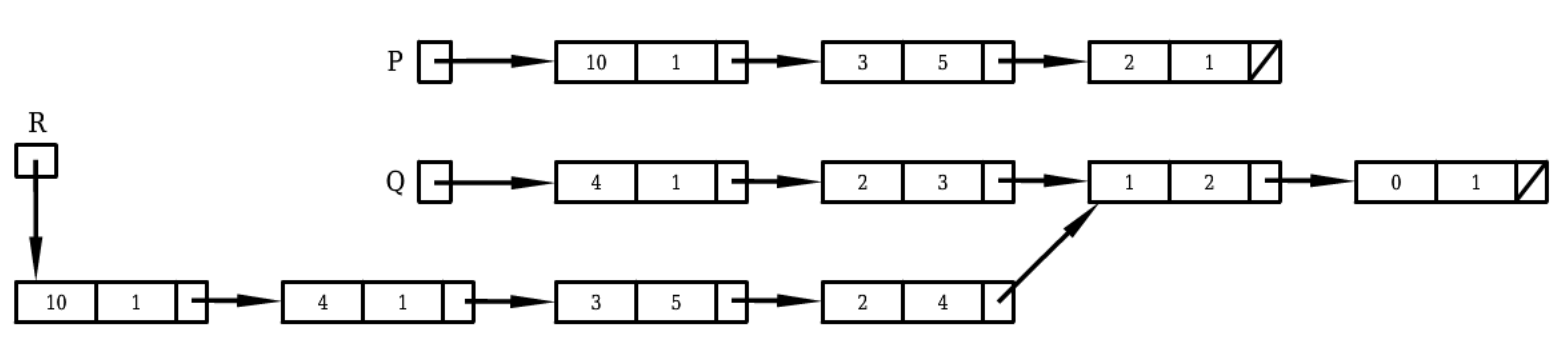
\includegraphics[width=12cm]{./img/Pic6.png}
\end{framed}
\caption{Сложение двух многочленов, представленных списками}
\end{figure}

\renewcommand{\figurename}{Алгоритм}

\newpage

\lhead{\small\textit{Решения упражнений}}
\rhead{161}

На рис. 6 видим схему памяти, представляющую три многочлена: $P =$ \linebreak $X^{10} + 5X^3 + X^2$, $Q = X^4 + 3X^2 + 2X + 1$ и $R = P + Q$, вычисленный с помощью предыдущего метода. Каждый элемент списка на этом рисунке представлен в виде тройки (степень, коэффициент, указатель). Этот метод реализован в алгоритме 18.

Построение списка, содержащего частичные последовательные результаты, осуществляется по возрастанию степеней. Следовательно, если один из списков исчерпался, нужно перевернуть промежуточный результат \linebreak прежде, чем присоединить хвост другого списка. Это делает подпрограмма \textit{Reverse\_Append}, которую можно поместить в пакет, разработанный в \linebreak упражнении 30. Эта функция реализована, начиная с примитивов управления списком: \textit{Head, Tail, Construct и Is\_Null}.

\begin{lstlisting} [language=C,
					basicstyle=\small,
					linewidth=14cm,
					mathescape=true,
					frame=none]
	$\textit{List}$ Reverse_Append($\textit{List}$ The_List, $\textit{List}$ And_The_List) {
		$\textit{List}$ x = The_List;
		$\textit{List}$ y = And_The_List;
		while (!Is_Null(x)) {
			y = Construct(x->Element, y);
			x = Tail(x);
		}
		return y;
	}
\end{lstlisting}

\begin{lstlisting} [language=C,
					basicstyle=\small,
					mathescape=true,
					caption=Сумма двух разреженных многочленов]
	R = Null_List;
	while (1) {
		if (Is_Null(Q)) return Reverse_Append(R, P);
		else if (Is_Null(P)) return Reverse_Append(R, Q);
		if (Head(Q)->Degree > Head(P)->Degree) {
			R = Construct(Head(Q), R);
			Q = Tail(Q);
		} else if (Head(P)->Degree > Head(Q)->Degree) {
			R = Construct(Head(P), R);
			P = Tail(P);
		} else {
			x = Head(P)->Coefficient + Head(Q)->Coefficient;
			if (x != 0)
				R = Construct(New_Element$\footnotemark$(Head(P)->Degree, x), R);
			P = Tail(P);
			Q = Tail(Q);
		}
	}
\end{lstlisting}

\footnotetext{\textit{New\_Element()} - "конструктор" объекта \textit{Element}. (Прим. редактора)}

Порядок многочлена есть его наименьшая степень, а его высота, обо- \linebreak

\newpage

\lhead{162}
\rhead{\small\textit{$I$ \quad Алгоритмика и программирование на языке Ада}}

\noindent
значаемая через $\sharp P$, — число ненулевых мономов в $P$. Если порядок $P$ больше порядка $Q$, то сложность алгоритма сложения прямо пропорциональна выражению:

\begin{center}
$\sharp P$ + число мономов многочлена $Q$ степени большей, чем порядок $P$.
\end{center}

\noindent
В этих вычислениях смешаны сложность просмотра списков и сложность вычисления арифметических операций — это вполне разумно в случае многочленов с небольшими целыми коэффициентами, но нереалистично, если арифметика коэффициентов более сложна.

\paragraph{32. Умножение многочленов, представленных списками} \mbox{}\\

Пусть $P = \sum a_i X^{\alpha_i}$, где $\alpha_i < \alpha_{i + 1}$ и $Q$ — два многочлена, которые требуется перемножить. Их произведение может вычисляться по формуле $R = \sum a_i X^{\alpha_i}Q$, если предполагается осуществлять умножение, следуя представлению $P$ в виде суммы одночленов. Легко видеть, что было бы удобно использовать функцию, реализующую умножение одночлена на многочлен. Эта функция легко и эффективно  реализуется, если воспользоваться более общей функцией, оперирующей списками таким образом, что на основании данного списка и некоторого преобразования его элементов она выдает новый список, полученный дублированием и преобразованием исходного списка.

\begin{lstlisting} [language=C,
					linewidth=10cm,
					mathescape=true,
					frame=none]
	$\textit{Element}$ Transform($\textit{Element}$ The_Element);
	$\textit{List}$ Map_List($\textit{List}$ The_List);
\end{lstlisting}

Реализация этого несколько особенного итерационного цикла — каково должно быть тело пакета \textit{List\_Handler}, если стремиться к эффективной реализации? — предлагается читателю. Чтобы получить функцию умножения одночлена на многочлен, конкретизируем функцию \textit{Map\_List} с помощью следующей процедуры преобразования\footnote{Трудноконвертируемый в Си код. Приведен оригинал на Ada для лучшего понимания. \textit{(Прим. редактора)}}:

\begin{lstlisting} [language=Ada,
					basicstyle=\small,
					linewidth=13cm,
					mathescape=true,
					frame=none]
	function $\textit{Multiply (M : Monomial, P : Polynomial)}$
			return $\textit{Polynomial}$ is
		function $\textit{Multiply\_M\_By (M\_1 : Monomial)}$ return $\textit{Monomial}$;
		function $\textit{Result}$ is new $\textit{Map\_List (Transform => Multiply\_M\_By)}$;
		function $\textit{Multiply\_M\_By (M\_1 : Monomial)}$ is
		begin
			return $\textit{(Degree => M.Degree + M\_1.Degree,}$
							$\textit{Coefficient => M.Coefficient * M\_1.Coefficient)}$;
		end $\textit{Multiply\_M\_By}$
	begin
		return $\textit{Result(P)}$;
	end $\textit{Multiply}$;
\end{lstlisting}

% \end{106/145-162}
%163-180 Мищенко
%\documentclass{../../template/mai_book}

\defaultfontfeatures{Mapping=tex-text}
\setdefaultlanguage{russian}

\usepackage{dsfont}% for mathds and more
\usepackage{scrextend}

%\clearpage
%\setcounter{page}{7} % ВОТ ТУТ ЗАДАТЬ СТРАНИЦУ
%\setcounter{thesection}{5} % ТАК ЗАДАВАТЬ ГЛАВЫ, ПАРАГРАФЫ И ПРОЧЕЕ.
% Эти счетчики достаточно задать один раз, обновляются дальше сами
% \newtop{ЗАГОЛОВОК}  юзать чтобы вручную поменть заголовок вверху страници

\begin{document}
%//////////////////////////////////////
%//Begin of 181 page
%//////////////////////////////////////
%\newtop{II-1.2 $\:$ Что такое факториальное кольцо?}

\noindent \textit{нуля, то оба элемента равны } \textbf{с точностью до обратимого элемента}\textit{,
т.е. существует $\text{\textepsilon}\in\:U(A)$, такой, что $a=\text{\textepsilon}\:\!b$.}

\textit{($iii$) Элемент р $\in$ А называется} \textbf{неприводимым}\textit{, если он не является ни нулевым, ни обратимым и если его единственными делителями являются 1 и р. Более точно: р неприводим тогда и только тогда, когда d | р $\Rightarrow$ d \textasciitilde$\:$ 1 или d \textasciitilde$\:$ р. Это свойство равносильно тому, что идеал Ар является максимальным в множестве} \textbf{однопорожденных}\textit{ (т.е глав­ных) идеалов в А, отличных от А и \{0\}.}

\textit{($iv$) Если кольцо А без делителей нуля, то р — неприводимый эле­мент тогда и только тогда, когда из р = de следует, что d или е — обратимый элемент в А.}

\section{\large 1.2 Что такое факториальное кольцо?}

Теперь можно дать точное определение структуры колец, обобщающей в какой-то мере структуру кольца $\mathds{Z}$ целых чисел.

\begin{determ}[факториальность]
\textit {\indent} Кольцо А называется факториальным, если оно не имеет делителей нуля и если оно удовлетворяет основной теореме арифметики, что, формально, выражается следующим образом: \newline \indent($i$) Наличие разложения на неприводимые множители:
\begin{align*}
\forall a \in A^* \backslash U(A),\,\exists p_1 ,p_2 ,\dots,p_n , \text{\textit{неприводимые}} \\ 
\text{\textit{и такие, что}}\: a = p_1 p_2 \dots p_n . 
\end{align*}
\indent ($ii$) Единственность такого разложения:
\begin{align*}
p_1 p_2 \dots p_n \sim_A q_1 q_2 \dots q_m (p_i , q_j \text{\textit{неприводимые }}\;\Rightarrow \\
n = m \:\text{и}\: \exists \sigma, \text{\textit{перестановка на }}[1, n]\text{\textit{, такая, что }} \\
p_i \sim_A q_{q(i)} (1 \leqslant i \leqslant n) \text{.}
\end{align*}
\end{determ}

В дальнейшем мы рассмотрим критерии, позволяющие распознать факториальность кольца. В настоящий момент читатель должен пове­рить, что это понятие не «бессодержательное», т.е. класс факториаль­ных колец сравнительно широк. Прежде, чем продолжать дальнейшее изучение делимости, укажем одно арифметическое приложение факториальности.

\newpage
%//////////////////////////////////////
%//Begin of 182 page
%//////////////////////////////////////
%\setcounter{page}{182}
%\newtop{II-1 $\:$ Обобщение арифметики целых чисел}

\subsection{\large 1.3 Обобщать арифметику целых чисел: зачем?}

\noindent Абстрагирование от конкретной ситуации позволяет математику отследить влияние основных параметров, влияющих на ситуацию, и диапазон их изменения. Более того, часто происходит так, что свойства обобщенной ситуации оказываются полезными для изучения базовой ситуации. Вот пример, когда арифметика подкольца кольца $\mathds{Z}$ оказывает влияние на арифметику в $\mathds{Z}$.
\newline \indent Рассмотрим для этого кольцо целых гауссовых чисел $\mathds{Z}[i] = \mathds{Z} + i\mathds{Z} =$\newline $\{x + iy | (x, у) \in \mathds{Z} \times \mathds{Z}\}$. Очевидно, $\mathds{Z}[i]$ — подкольцо поля $\mathds{C}$ комплексных чисел, выдерживающее операцию сопряжения $z \rightarrow \bar{z}$. Поэтому операция сопряжения индуцирует инволютивный автоморфизм в $\mathds{Z}[i]$, в котором $\mathds{Z}$ является множеством неподвижных точек, и позволяет оснастить $\mathds{Z}[i]$ мультипликативной нормой $N : \mathds{Z}[i] \rightarrow \mathds{N}$, определяемой через $N(z) = z\bar{z}$, для $z \in \mathds{Z}[i]$. Другими словами, $N(x + iy) = x^2 + y^2 $ для всех $x , y \in \mathds{Z}$.

\begin{predl}
\textit{\indent} ($i$) Кольцо $\mathds{Z}[i]$ целых гауссовских чисел факториально. 
\newline \indent($ii$)  Пусть $z \in \mathds{Z}[i]$ — неприводим в $\mathds{Z}$ и не ассоциирован с элементом из $\mathds{Z}$. Тогда $N(z)$ является простым числом в $\mathds{Z}$.
\end{predl}

\begin{myproof}
Пункт $(i)$ следует из евклидовости $\mathds{Z}[i]$ (см. раздел 3.1) и того, что всякое евклидово кольцо без делителей нуля факториально (см. раздел 3.5). \newline Что касается $(ii)$, то мы покажем, что разложение $rs$ числа $N(z)$ в $\mathds{Z}$ тривиально. Сначала предположим, что ни r, ни s не обратимы в $\mathds{Z}[i]$. Пусть $n$ (соответственно, $m$) — длина разложения на простые множители для $r$ (соответственно, для $s$). Так как $z\bar{z}$ является простым разложением для $N(z)$ (напомним, что $z$ и $\bar{z}$ неприводимы в $\mathds{Z}[i]$), то из единственности разложения на неприводимые множители следует, что $m + n = 2$, откуда $n = m = 1$, т.е. $r$ и $s$ — неприводимые в $\mathds{Z}[i]$. Из единственности следует, что $z \sim_{mathds{Z}[i]} r$  или $z \sim_{mathds{Z}[i]} s$ , что противоречит предположению относительно $z$ ($z$ не ассоциирован с элементом из $\mathds{Z}$). Следовательно, хотя бы один из двух элементов $r$ и $s$ является обратимым в $\mathds{Z}[i]$. Но из $r \in U(\mathds{Z}[i])$ следует, что $N(r) \in U(\mathds{Z})$. Так как $N(r) = r^2$ и $N(s) = s^2$ , то имеем $r = \pm 1$ или $s = \pm 1$. \\
\end{myproof}

\begin{mynotice}
\noindent В доказательстве, приведенном выше, мы использовали (кроме факториальности кольца) только наличие мультипликативной нормы со значениями в $\mathds{Z}$ (фактически, в $\mathds{N}$, хотя это

\newpage
%//////////////////////////////////////
%//Begin of 183 page
%//////////////////////////////////////
%\newtop{II-1.3 $\:$ Обобщать арифметику целых чисел: зачем?}

\noindent и не важно). В то же время вид единиц в $\mathds{Z}[i]$ не был использован. Кроме того, существование мультипликативной нормы основано, главным образом, на существовании инволютивного автоморфизма $z \rightarrow \bar{z}$, для которого $\mathds{Z}$ является множеством неподвижных точек. Такой тип доказательства применим и в других ситуациях.
\end{mynotice}

\begin{predl}
\textit{\indent} Элемент вида $x^2 + y^2$ из $\mathds{N}$, где $x \in \mathds{N}$ и $y \in \mathds{N}$ взаимно просты, назовем точной суммой двух квадратов. Тогда всякий делитель (из $\mathds{N}$) точной суммы двух квадратов сам является точной суммой двух квадратов.
\end{predl}

\begin{myproof}
Заметим сначала, что «общая» сумма двух квадратов может иметь делители, о которых ничего сказать нельзя (достаточно рассмотреть сумму виде $(\lambda x)^2 + (\lambda y)^2 $ и тогда $\lambda$ — такой делитель). Поэтому утверждение о взаимной простоте $x + iy$ в произведение неприводимых в $\mathds{Z}[i]: x + iy = \pi_1 \dots \pi_n $ , где $\pi_j $ неприводимы. Это разложение индуцирует разложение $x^2 + y^2:$
\begin{align}
x^2 + y^2 = N(x + iy) = N(\pi_1 )N(\pi_2) \dots N(\pi_n )\text{.}
\end{align}
Заметим, что ни одно из $\pi_j$ не ассоциировано с элементом из $mathds{Z}$ (так как $x$ и $y$ взаимно просты). Согласно предшествующей лемме, $N(\pi_j )$ является простым элементом $\mathds{Z}$. Следовательно, разложение $(1)$ есть разложение (в $\mathds{Z}$) $x^2 + y^2$ на простые множители. Если $d \in \mathds{N}$ — делитель $x^2 + y^2$, то существует такое подмножество $J \subset [1,n]$, что
\begin{align*}
d = \prod_{j \in J}\: N(\pi_j) = N\Biggl(\prod_{j \in J} \pi_j \Biggr) = u^2 + v^2\text{, где } u + iv = \prod_{j \in J} \pi_j \text{.} 
\end{align*}
Откуда следует, что $d$ есть сумма двух квадратов. Так как $u + iv$ является делителем в $\mathds{Z}[i]$ числа $x + iy$, то эта сумма точная.\\
\end{myproof}

\begin{mynote}% 1em left, 2em right
\textit{\indent} Зная, что кольцо $\mathds{Z}[\sqrt{—2}] = \mathds{Z} + i\sqrt{2}\mathds{Z} = \{x + \sqrt{—2}у, (x,y) \in \mathds{Z}\times\mathds{Z}\}$ факториально, можно доказать небанальный результат, касающийся сумм $x^2 + 2y^2$ , где $(x,y) \in \mathds{N}\times\mathds{N}$. Это обобщенная точка зрения математика $\dots$

\newpage
%//////////////////////////////////////
%//Begin of 184 page
%//////////////////////////////////////
%\newtop{II-1 $\:$ Обобщение арифметики целых чисел}
\noindent Кстати: существует аналогичный результат для сумм вида $x^2 - 2y^2$, связанный с кольцом $\mathds{Z}[\sqrt{2}] = \mathds{Z} + \sqrt{2}\mathds{Z}$. Предложложив, что кольцо факториально, можно доказать, для взаимно простых $x,y \in \mathds{Z}$ следующий результат:
\begin{align*}
d \in \mathds{Z}, d|x^2 - 2y^2 \Rightarrow \exists u \in \mathds{Z}\text{,}v \in \mathds{Z} \:\text{такие, что } d = u^2 - 2v^2\text{.}
\end{align*}
Начнём с определения инволютивного автоморфизма $\mathds{Z}[\sqrt{2}]$ (которое в этом случае уже не связано с операцией сопряжения в $\mathds{C}$), затем введём норму (со значением в $\mathds{Z}$ на этот раз)$\dots$, остерегаясь обратимого элемента $-1 \in \mathds{Z}$. Новая ступень преодолена. \newline \indent Однако аналогичного феномена для сумм вида $x^2 + 3y^2$ в кольце $\mathds{Z}[\sqrt{-3}]$ не наблюдается. Не путайте кольцо $\mathds{Z}[j]$ целых чисел и кольца $\mathds{Q}[\sqrt{-3}]$. Оно не факториально!\\
\end{mynote}

Пусть $p \in \mathds{N} \backslash \{2\}$ — простое число, являющееся суммой двух квадратов. Легко проверить, рассматривая $\mathds{Z}/4\mathds{Z}$, что $p \equiv 1\:(mod\:4)$. Вот обратное утверждение: 

\begin{sled}
\textit{\indent} Пусть $p \in \mathds{N}$ — простое число, удовлетворяющее соотношению $p \equiv 1\:(mod\:4)$. Тогда $p$ является суммой двух квадратов.
\end{sled}

\begin{myproof}
Сравнение Вильсона для всякого простого $p$:
\begin{align*}
(p - 1)!\equiv -1\:(mod\:p)
\end{align*}
получается при помощи перегруппирования в произведении $1 \times 2 \times \dots \times (p-1)$ каждого сомножителя со своим обратным по модулю $p$. Если $p \neq 2$, то, перегруппировывая в том же произведении вместе числа $i$ и $(p - i)$, получаем формулу
\begin{align*}
(-1)^{(p-1)/2} \Biggl(\Biggl(\frac{p-1}{2}\Biggr)!\Biggr)^2 \equiv -1\:(mod\:p)\text{.}
\end{align*}
В частности, если $p \equiv 1 (mod 4)$ и если $x = (\frac{p-1}{2})!$, то $x^2 \equiv —1\:(mod\:p)$ или, что то же самое, $p | (x^2 + 1)$. Простое $p$ делит точную сумму двух квадратов и, следовательно, само является суммой двух квадратов. \newline Можно заметить, что главный этап доказательства состоит в~ утверждении, что $—1$ является квадратом по модулю $p$, где $p$ — число вида $4n + 1$. Этот результат, прямое доказательство которого было только что получено, будет углублен позже в части, посвященной квадратичным вычетам.
\end{myproof}

\newpage
%//////////////////////////////////////
%//Begin of 185 page
%//////////////////////////////////////

Закончим раздел сводкой результатов, относящихся к группе единиц и неприводимым элементам в $\mathds{Z}[i]$ (результаты, содержащие, в частности, пункт ($ii$) теоремы 5). Указанные результаты позволяют лучше понять новое кольцо, удовлетворяющее основной теореме арифметики, обобщающее некоторые кольца, являющиеся квадратичными расширениями, например $\mathds{Z}[\sqrt{2}]$ или $\mathds{Z}[\sqrt{2}]$, но не все! \newline \indent Пусть $p \in \mathds{Z}$. Если $p$ неприводимо в $\mathds{Z}[i]$, то оно тем более неприводимо в $\mathds{Z}$ (это простое число из $\mathds{Z}$). Следующее предложение содержит одну из возможных обратных теорем:

\begin{predl}
\textit{\indent} ($i$) $U(\mathds{Z}[i]) = \{z \in \mathds{Z}[i] | N(z) = 1\} = \{+1,-1,+i,-i\}$. \newline \indent ($ii$) Если $p$ — простое в $\mathds{N}$, то $p$ неприводимо в $\mathds{Z}[i]$ тогда и только тогда, когда оно не является нормой $N(z)$ для $z \in \mathds{Z}[i]$ (что эквивалентно $p \equiv 3\:(mod\:4)$). \newline \indent ($iii$) Пусть $z \in \mathds{Z}[i]$. Элемент $z$ является неприводимым в $\mathds{Z}[i]$ и не ассоциированным с элементом из $\mathds{Z}$ тогда и только тогда, когда $N(z)$ — простое число в $\mathds{Z}.$
\end{predl}

\noindent \textbf{ \large \textit{Несколько примеров}}
\begin{enumerate}
\item Число $5$ — простое в $\mathds{Z}$, не неприводимое в $\mathds{Z}[i]$, так как существует нетривиальное разложение $5 = 1^2 + 2^2 = (1 + 2i)(1 — 2i)$
\item В $\mathds{Z}[i] 2$ разлагается в сумму двух равных квадратов и почти является квадратом: $2 = 1^2  + 1^2  = (1 + i)(l — i) = —i(1 + i)^2 \sim_{\mathds{Z}[i]} (1 + i)^2.$
\item В $\mathds{Z}[i]$ еще неприводимо $2 + Зi$, так как $N(2 + Зi) = 13$ — простое число в $\mathds{Z}$.
\item Простые числа $181$, $281$ и $601$, сравнимые с $1$ по модулю $4$, имеют представление в виде суммы двух квадратов: $181 = 9^2 + 10^2$, $281 = 5^2 + 16^2$, и $601 = 5^2 + 24^2$.\\
\end{enumerate}

\begin{myproof}[Доказательство предложения 8]
$\;\;\;\;$ Пункт ($i$) вытекает из равенства
\begin{align*}
U(\mathds{Z}[i]) = \{z \in \mathds{Z}[i]\:|\:N(z) \text{обратим в}\:\mathds{Z}\:\} = \{+1,-1,+i,-i\}\text{.}
\end{align*}
\indent Докажем ($ii$), рассматривая простое число $р$ из $\mathds{N}$. Если $p$ является нормой $N(z)$, то имеется нетривиальная факторизация: $p = z\bar{z}$, которая показывает, что $p$ не является неприводимым в $\mathds{Z}[i]$.

\newpage
%//////////////////////////////////////
%//Begin of 186 page
%//////////////////////////////////////

Обратно, если $p$ не является неприводимым в $\mathds{Z}[i]$, то имеется его разложение на неприводимые в $\mathds{Z}[i]:\:р = \pi_1 \pi_2 \dots \pi_n$ с $n \geqslant 2$. Применяя норму, получаем: $р^2 = N(\pi_1) N(\pi_2) \dots N(\pi_n)$ дает нетривиальное разложение $p^2$ в $\mathds{Z}$. Отсюда $n = 2$, $N(\pi_1) = p$ и $N(\pi_2) = p$.\newline \indent Второй результат о равносильности — следствие первого. \newline \indent ($iii$) Пусть $z \in \mathds{Z}[i]$ такое, что $N(z)$ — простое число в $\mathds{N}$. Из разложения $z = z_1 z_2$, где $z_1$ и $z_2$ принадлежат $\mathds{Z}[i]$, получаем, применяя норму, что $N(z) = N(z_1 ) N(z_2 )$. Это — разложение простого числа $N(z)$ в $\mathds{Z}$. Оно непременно тривиально. Следовательно, тому, что исходное разложение является разложением неприводимого элемента $z$ из $\mathds{Z}[i]$ (и подтверждает его неассоциированность с элементом из $\mathds{Z}$). Обратное уже было доказано в предложении 5.
\end{myproof}

\section{\large{2 Эементарные~ свойства теории~ делимости}}

Мы займемся нахождением общих критериев факториальности колец. Эти критерии устанавливаются совершенно естественным путем и ба­зируются на основных понятиях теории делимости: нётеровости кольца и свойстве Гаусса.

\subsection{2.1 Существование и единственность разложения на \newline простые~ множители}

\subsection{(9) Предложение.}
\textit{\indent Пусть любая бесконечно неубывающая последовательность главных (т.е. порожденных одним элементом) идеалов кольца $A$ без делителей нуля стабилизируется (т.е. становится постоянной, начиная с некоторого ее члена). Тогда кольцо $A$ удовлетворяет условию существования разложения на неприводимые множители.}

\begin{myproof}
Допустим, что условие на главные идеалы выполнено. Предположим противное: существует $x_0 \in A^* \backslash U(A)$, не являющийся произведением неприводимых. Элемент хо тем более не является неприводимым и поэтому имеет нетривиальное разложение $x_0 = x_1 y_1$, где $x_1$ и $y_1$ необратимы. Один из двух элементов $x_1$ или $y_1$ не представим в виде произведения неприводимых (иначе $x_0$ обладает разложением в произведение неприводимых). Пусть это будет $x_1$. Значит имеем строгое включение $A x_0 \varsubsetneq A x_1$. Тогда это рассуждение можно

\newpage
%//////////////////////////////////////
%//Begin of 187 page
%//////////////////////////////////////
\noindent повторить для $x_1$, что дает другое точное включение того же типа, что и первое: $A x_1 \varsubsetneq A x_2$ с $x_2$, не являющимся произведением неприводимых. Ясно, что можно построить бесконечную последовательность главных идеалов, которая не может стабилизироваться.
\end{myproof}

Следующее предложение связано с единственностью разложения на неприводимые множители. Доказательство является простой формальностью и предоставим его читателю.

\begin{predl}
\textit{\indent} Пусть $A$ — кольцо без делителей нуля, удовлетворяющее условию существования разложения в произведение неприводимых. Тогда $A$ обладает свойством единственности разложения (т.е. является \textbf{факториальным}), если для любого неприводимого $p$ выполнено следующее свойство: если $p$ делит $ab$, то $p\:|\:a$ или $p\:|\:b$ (значит $p$ может рассматриваться как простой элемент).
\end{predl}

\subsection{\large 2.2 НОД и взаимно простые элементы}

\begin{determ}
\textit{\indent} ($i$) Элемент $d \in A$, являющийся общим делителем $a$ и $b$, называется НОД $a$ и $b$, если всякий другой делитель $\delta$ элементов $a$ и $b$ является делителем $d$. В кратком виде это выражается следующей эквивалентностью:
\begin{align*}
d\:\text{есть НОД}\:a\:\text{и}\:b\:\text{тогда и только тогда, когда}\:[\delta\:|\:d\:\Longleftrightarrow\:\delta\:|\:a\:\text{и}\:\delta\:|\:b]\text{.}
\end{align*}
В этом случае идеал $Ad$ является единственным: действительно, сказать, что $d = $НОД$(a,b)$ равносильно тому, что идеал $Ad$ есть верхняя грань для множества $\{Aa, Ab\}$ главных идеалов. \newline \indent В дальнейшем будем использовать обозначения $d = $НОД$(a, b)$ или $a = a \wedge b$, помня, что в общем случае НОД — не единственный элемент. \newline \indent ($ii$) Элементы $a$ и $b$ будут называться \textbf{взаимно простыми} , если 1 является НОД $a$ и $b$ (равносильным образом, это означает, что только единицы $A$ — суть общие делители для $a$ и $b$).
\end{determ}

Существуют кольца, обладающие парами элементов, не имеющими наибольшего общего делителя. Покажем это.

\textit{\textbf{Кольцо $A = \mathds{Z}[\sqrt{-5}]$}}

Рассмотрим кольцо $A = \mathds{Z}[\sqrt{-5}] = \{x + iy\sqrt{5}, x, y \in \mathds{Z}\}$. Это множество есть подкольцо поля С с обычными операциями сложения и

\newpage
%//////////////////////////////////////
%//Begin of 188 page
%//////////////////////////////////////
\setcounter{page}{188}
%\newtop{II-2 $\:$ Элементарные свойства теории делимости}
\noindent умножения и потому без делителей нуля. Операция сложения в $\mathds{C}$ инду­
цирует инволютивный автоморфизм $\sigma \mathds{Z}[\sqrt{-5}]:\sigma(x+y\sqrt{5}) = x - y\sqrt{5}$,
и дает возможность определить в $\mathds{Z}[\sqrt{-5}]$ мультипликативную алгебра­
ическую норму со значениями в $\mathds{N}$, определяемую через $N(z) = z\sigma(z)$.
Другими словами, $N(x + y\sqrt{-5}) = x^2 + 5y^2$. Группа единиц в $\mathds{Z}[\sqrt{-5}]$ следующая:
\begin{align*}
U(\mathds{Z}[\sqrt{-5}]) =  \{z \in \mathds{Z}[\sqrt{-5}]\:\text{с}\:N(z) = 1\} = \{\pm 1\}\text{.}
\end{align*}
\indent Элемент $2$ неприводим в этом кольце. Действительно, из соотношения $2 = uv$ следовало бы равенство $4 = N(u)N(v)$. Так как $2$ не представимо в виде $x^2 + 5y^2$, то $2$ не является нормой. Из этого ясно, что $N(u) = 1$ или $N(v) = 1$: $u$ или $v$ обратим, а, следовательно, $2$ неприводим. Таким же образом можно показать, что элементы $3$, $1 + \sqrt{5}$ и $1 - \sqrt{5}$ неприводимы. Однако для них выполнено равенство $2 \times 3 = (1 + \sqrt{5} )\times(1 - \sqrt{5})$. Как грустно: $4$ сомножителя, встречающихся здесь, неприводимы! Понятно, что в кольце $\mathds{Z}[\sqrt{-5}]$ основная теорема арифметики не имеет места. \newline \indent Если положим $a = 1 + \sqrt{-5}$ , $b = 1 — \sqrt{-5}$, то это равенство имеет другое необычное следствие: $2 | ab$, $2$ неприводимо, но $2$ не делит ни $a$, ни $b$! Беда не приходит одна. В результате предыдущей патологии элементы $2a$ и $ab$ не имеют НОД в $\mathds{Z}[\sqrt{-5}]$. Допустим, что $d$ — общий делитель $2a$ и $ab$. Тогда $d\:|\:2a$ и $а\:|\:d$, что приводит к заключению $(\frac{d}{a} | 2$. Так как $2$ неприводимо, то $d \sim_A a $ или $d \sim_A 2a$. Но а не может быть НОД (он не делится на общий делитель с $2$), а $2a$ — тем более ($b$ не делится на $2$, $ab$ не делится на $2a$), что приводит к противоречию.

\subsection{\large 2.3 Выделение понятия}
\noindent Мы уже рассмотрели два важных свойства. Одно связано с наличием разложения на неприводимые множители, другое — с единственностью разложения. Это дает повод к следующим определениям:

\begin{determ}[свойство Гаусса]
\textit{\indent} Элемент $p$ кольца $A$ \textbf{называется простым}, если он отличен от нуля, не является обратимым и удовлетворяет условию: $p | ab \rightarrow p | a$ или $p | b$, что можно выразить по-другому: факторкольцо $A/Ap$ не имеет делителей нуля.
\end{determ}

\begin{determ}[упорядоченное нётерово множество]
\textit{\indent} Упорядоченное множество $X$ называется нётеровым, если всякая бесконечная возрастающая последовательность стабилизируется.
\end{determ}

\newpage
%//////////////////////////////////////
%//Begin of 189 page
%//////////////////////////////////////
\begin{determ}[нётерово кольцо]
\textit{\indent} Кольцо $A$ называется нётеровым, если множество идеалов этого кольца, упорядоченное по включению, является нётеровым. Другими словами, всякая бесконечная возрастающая последовательность идеалов постоянна, начиная с некоторого номера.
\end{determ}

По определению (или почти по определению) для факториального кольца понятия простого и неприводимого элемента совпадают. Между прочим, в кольце без делителей нуля имеет место следующее свойство:

\begin{determ}
\textit{\indent} В кольце без делителей нуля простой элемент неприводим. Обратное, вообще говоря, неверно.
\end{determ}

\begin{determ}[принцип нётеровой индукции]
\textit{\indent} Упорядоченное множество $X$ нётерово тогда и только тогда, когда всякое непустое подмножество $Y$ в $X$ обладает максимальным элементом, содержащимся в $Y$ (элемент $y \in Y$ называется максимальным в $Y$, если не существует $z \in Y$, для которого $z > y$).
\end{determ}

\begin{myproof}
Допустим, что $X$ нётерово и $Y \subset X$ — непустое подмножество $X$ без максимального элемента. Пусть $x_0 \in Y$. Так как $x_0$ не максимальный в $Y$ , то найдется $x_i \in Y$, такой, что $x_0 < x_1$. Так как $x_1$ не максимален в $Y$, то можно построить $x_2$, такой, что $x_i < x_2$, $x_2 \in Y$. Это вам ничего не напоминает? \newline Обратно, пусть $(x_n)_{n \in \mathds{N}}$ — возрастающая последовательность элементов из $X$. Если $x_m$ — максимальный элемент множества $\{x_n,n \in \mathds{N}\}$, то последовательность $(x_n)_{n \in \mathds{N}}$ стабилизируется, начиная с номера $m$.\\
\end{myproof}

\begin{determ}[связь между нётеровостью и конечностью колец]
\textit{\indent} Кольцо $A$ является нётеровым, тогда и только тогда, когда всякий идеал в $A$ конечного типа (т.е. порожден конечным числом элементов).
\end{determ}

\begin{myproof}
Допустим, что всякий идеал конечного типа, и пусть $(I_n)_{n \in \mathds{N}}$ — возрастающая последовательность идеалов. Объединение $I = \bigcup_{n \in \mathds{N}} I_n$ есть идеал, порожденный конечным подмножеством $\mathcal{F}$. Так как $(I_n)_{n \in \mathds{N}}$ возрастающая, то существует такое $m \in \mathds{N}$, что $\mathcal{F} \subset I_m$. Отсюда получаем, что $I = I_m$, а, следовательно, начиная с номера $m$, последовательность $(I_n)_{n \in \mathds{N}}$ стабилизируется.

\newpage
%//////////////////////////////////////
%//Begin of 190 page
%//////////////////////////////////////
\noindent Обратно, предположим, что кольцо $A$ нётерово, содержащее идеал $I$, не являющийся идеалом конечного типа. Так как $I$ не является идеалом конечного типа, то $x_0 \in I$, затем $x_1 \in I \backslash A x_0$, затем $x_2 \in I \backslash (A x_0 + A x_1 )\:\dots$ Это приводит нас к наличию строго воэрастающей последовательности идеалов:
\begin{align*}
Ax_0 \varsubsetneq Ax_0 + Ax_1 \varsubsetneq Ax_0 + Ax_1 + Ax_2 \varsubsetneq \dots \\
\varsubsetneq Ax_0 + Ax_1 + \dots + Ax_n \varsubsetneq \dots\text{,}
\end{align*}
что заканчивает доказательство.
\end{myproof}
Прежде чем перейти к вещам, более конкретным, забежим вперед в главу III и приведем несколько результатов о нётеровых модулях. Конечно, нётеров модуль — это такой модуль, в котором всякая возрастающая последовательность подмодулей стабилизируется, или, иначе, всякий подмодуль является подмодулем конечного типа. Для того чтобы связать сказанное с предыдущим, заметим, что идеалы кольца являются его подмодулями.

\begin{predl}
\textit{\indent} ($i$) Пусть $A$ — кольцо. Если $A$-модуль $E$ — нётеров, то для всякого подмодуля $F$ модуля $E$ $A$-модули $E/F$ и $F$ нётеровы. Обратно, если в $A$-модуле $E$ есть такой нётеров подмодуль $F$, что $E/F$ нётеров, то и $E$ — нётеров.
\end{predl}

\begin{myproof}
Доказательство первого результата очень просто. Действительно, всякая возрастающая последовательность подмодулей $F$ является также возрастающей последовательностью подмодулей в $E$. Заметим также, что подмодули $E/F$ есть образы подмодулей $E$, содержащие $F$. \newline Обратное утверждение доставляет больше забот. Нельзя пользоваться теми же рассуждениями, что в векторном пространстве, и предполагать, например, что $E \simeq E/F \oplus F$. \newline Рассмотрим отображение, которое каждому подмодулю $G$ в $E$ ставит в соответствие пару $(G + F, G \cap F)$. Это отображение порождает строго возрастающую последовательность. Действительно, рассмотрим два подмодуля $G' \subset G$, такие, что $G' + F = G + F$ и $G' \cap F = G \cap F$. Пусть элемент $x \in G$. Тогда $x = y + z$, где $y \in G', z \in F$. Так как $G' \cap G$, то $y \in G$ и, значит, $z \in G$. Однако $G' \cap F = G \cap F$, откуда $z \in G'$, и потому $x \in G'$. Таким образом, всякая строго возрастающая последовательность модулей в $E$

\newpage
%//////////////////////////////////////
%//Begin of 191 page
%//////////////////////////////////////
\noindent порождает строго возрастающую последовательность подмодулей в $(E + F)/F$ и $E \cap F$. Догадаемся о продолжении$\dots$
\end{myproof}

\begin{predl}
\textit{\indent} Если $E$ и $F$ — два $A$-модуля, то $E \times F$ нётеров модуль тогда, и только тогда, когда таковыми являются $E$ и $F$.
\end{predl}

\begin{myproof}
Проектируя $E \times F$ на каждый из подмодулей $E$ и $F$, получаем необходимость условия. Для доказательства обратного достаточно заметить, что $E \simeq E \times F / \{0\} \times F$ и применить предыдущее предложение.
\end{myproof}

\subsection{\large 2.4 Соотношение Безу}

\begin{predl}
\textit{\indent} ($i$) Пусть $a$, $b$ и $d$ — элементы кольца $A$, связанные соотношением \newline $Ad = Aa + Ab$. Тогда $d$ = НОД$(a, b)$. \newline \indent($ii$) Пусть $A$ — кольцо, в котором сумма двух главных идеалов есть главный идеал. Тогда всякий неприводимый элемент $A$ является простым элементом (т.е. удовлетворяет свойству Гаусса).
\end{predl}

\begin{myproof}
($i$) — простая формальность, в которой нет ничего удивительного. Действительно, $Aa + Ab$ есть верхняя грань для множества идеалов \newline $\{Aa, Ab\}$.\newline \newline Чтобы доказать ($ii$), предположим, что $p$ неприводим в $A$, $a \in A$ и $b \in A$ таковы, что $p | ab$. Допустим, к примеру, что $p$ не делит $a$. Тогда $Ap \varsubsetneq Ap + Aa$ и, значит, $Ap + Aa$ есть главный идеал. Из максимальности $Ap$ среди главных идеалов следует, что $Ap + Aa = A$, и поэтому выполнено соотношение Безу $1 = up + va$, из которого выводим $b = upb + vab$. Но тогда $p$ делит $b$.
\end{myproof}

\indent Подчеркнем роль, сыгранную соотношением Безу, связанную с НОД и свойством Гаусса в доказательстве предложения. Вот результат, приводящий к понятию максимального элемента.


\newpage
%//////////////////////////////////////
%//Begin of 192 page
%//////////////////////////////////////
\begin{determ}[кольцо Безу]
\textit{\indent} Кольцо А называется кольцом Безу, если сумма любых двух его главных идеалов является главным идеалом. Это эквивалентно тому, что всякий идеал конечного типа является главным.
\end{determ}

\begin{mynotice}
Введение понятия кольца Безу продиктовано соображениями удобства записи. Никакой теории колец Безу в этой книге не будет!
\end{mynotice}

\begin{predl}
Пусть $p$ — неприводимый элемент кольца Безу $A$. Тогда факторкольцо $A/Ap$ есть тело. Равносильным образом это означает, что идеал $Ap$ максимален среди всех идеалов (отличных от $A$). По-другому это можно выразить так: для любого $x \in A\backslash Ap$ существуют такие $u$ и $v$ из $A$, что $1 = ux + vp$.
\end{predl}

\begin{myproof}
Пусть $\xi$ — ненулевой элемент из $A\backslash Ap$, представляющийся элементом $x \in A\backslash Ap$. Тогда идеал $Ax + Ap$ есть главный идеал $Ad$, строго содержащий $Ap$. Отсюда $d | p$ и $d \nsim p$. Значит, $d \sim 1$, т.е. $1 \in Ax + Ap = A$. Поэтому найдутся такие $u$ и $v$, что $1 = ux + vp$, откуда, переходя к факторкольцу $A/Ap$, получаем $1 = \bar{ux} = \bar{u}\xi$, что доказывает обратимость $\xi$ в $A/Ap$. Отсюда следует, что $A/Ap$ — тело. \newline Читатель без труда проверит самостоятельно эквивалентность трех формулировок результата
\end{myproof}

\begin{determ}
\textit{\indent}Идеал $I$ кольца называется простым, если он отличен от $A$ и если для всякого произведения $ab \in I$ следует, что $a \in I$ или $b \in I$. Последнее равносильно тому, что факторкольцо $A/I$ не имеет делителей нуля. \newline \indent Идеал называется максимальным, если он максимален среди всех идеалов, отличных от $A$, или, что то же самое, факторкольцо $A/I$ является телом.
\end{determ}

\begin{mynotice}
Идеал $\{0\}$ простой тогда и только тогда, когда кольцо не имеет делителей нуля. Он максимален тогда и только тогда, когда кольцо является телом.
\end{mynotice}

\newpage
%//////////////////////////////////////
%//Begin of 193 page
%//////////////////////////////////////
\indent В качестве резюме:

\begin{predl}
\textit{\indent} ($i$) В кольце без делителей нуля всякий элемент, порождающий максимальный идеал, является простым, а каждый простой элемент неприводим. Два последние понятия (простой и неприводимый) совпадают в факториальном кольце, и все три понятия совпадают в кольце Везу. \newline \indent ($ii$) Элемент $p$ кольца $A$ простой тогда и только тогда, когда идеал $Ap$ простой и отличен от $\{0\}$. \newline \indent ($iii$) В любом кольце всякий максимальный идеал прост.
\end{predl}

\section{3 Евклидовы кольца с точки зрения эффективности}

Этот раздел посвящен изучению евклидовых колец, т.е. колец, обладающих евклидовым делением. Здесь можно будет найти точное определение данного понятия, элементарные свойства евклидовых колец, в частности, факториальности евклидовых колец без делителей нуля, алгоритм Евклида и его реализацию в языке Ада во всей его общности. Для более глубокого изучения необходимой математики читатель может обратиться к работе Самюэля $[159]$, являющейся очень толковыми легко читаемым руководством.

\subsection{3.1 Что такое евклидово кольцо?}

\begin{determ}
Евклидово деление в кольце $А$ есть оператор $A\times A^* \rightarrow A$, обозначаемый «$/$», для которого существует отображение $\phi$ кольца $A$ во вполне упорядоченное множество (т.е. множество, всякая непустая часть которого имеет наименьший элемент), удовлетворяющее соотношению:
\begin{align}
\forall(a,b) \in A \times A^*, \:\: \phi(a - b(a/b)) < \phi(b)
\end{align}
В этом случае говорят, что «$/$» евклидово для $\phi$. Отображение $\phi$ называется \textbf{алгоритмом Евклида}, если оно удовлетворяет свойству:
\begin{align}
\forall(a,b) \in A \times A^*, \exists(q,r) \in A \times A \:\text{такая, что}\: a = bq + r \: c \:\phi(r) < \phi(b)\text{.}
\end{align}
Эквивалентным образом, для всякого $b$ в $A^*$ существует такая система представителей в $A/Ab$, элементы $r$ которых удовлетворяют неравенству $\phi(r)<\phi(b)$.
\newpage
%//////////////////////////////////////
%//Begin of 194 page
%//////////////////////////////////////
\indent Кольцо $A$ (не обязательно без делителей нуля) называется евклидовым, если оно допускает евклидово деление «$/$» (в таком случае $A$ называется евклидовым для «$/$»), а также, что $A$ допускает евклидов алгоритм (в последнем случае говорят, что $A$ евклидово для $\phi$).
\end{determ}

\begin{mynotice}
Хотя в математике заостряется внимание на понятии евклидова алгоритма, именно эффективность евклидова деления позволяет вычислять НОД, находить коэффициенты Безу, и т.д. В какой-то мере приходится пожалеть о термине «алгоритм Евклида».\newline \indent Большинство евклидовых алгоритмов, используемых в математических учебниках, базируется на упорядоченности множества $\mathds{N}$(или на упорядочении множества, изоморфного $\mathds{N}$). Междупрочим, произведение колец $\mathds{Z} \times \mathds{Z}$ есть евклидово кольцо (имеющее делители нуля), не допускающее алгоритма Евклида с целыми значениями $[159]$. Гиблот в $[85]$ нашел аналогичный пример для кольца без делителей нуля.
\end{mynotice}

\begin{determ}
\textit{\indent} Пусть $A$ — евклидово кольцо для $\phi$. Скажем, что равенство типа $(3)$ есть \textbf{евклидово деление} (относительно $\phi$) $a$ на $b$, $q$ — частное евклидова деления, $r$ — остаток. Назовем оператором \textbf{взятия остатка} (для $\phi$) оператор $mod\::A \times A^* \rightarrow A$, удовлетворяющий соотношениям:
\begin{align*}
\phi(a\:mod\:b) < \phi(b)\;\text{и}\; a\:mod\:b\equiv a\:(mod\:b)\text{.}
\end{align*}
Каждое евклидово деление «$/$» определяет остаточный оператор\newline$a\;mod\;b = a - b \times (a/b)$, для $a \in A$ и $\b \in A^*$.
\end{determ}

\noindent \textbf{Примеры евклидовых алгоритмов на $\mathds{Z}$}
\newline \indent Кольцо $\mathds{Z}$ целых чисел является моделью для конструирования евклидовых колец. Вот два примера деления и евклидовых алгоритмов для $\mathds{Z}$.

\begin{enumerate}
\item Взятие абсолютного значения в $\mathds{Z}$ дает возможность построить алгоритм Евклида. Для $(a,\:b) \in \mathds{Z} \times \mathds{Z}^*$ можно записать $a = bq + r\:с\: |r| < |b|$ различными способами. Например, при $(a,b) = (—14,3)$ можно записать $—14 = 3 \times (-5) + 1$ и получить остаток, равный единице, или $—14 = 3 \times (-4) — 2$ с остатком, равным $-2$. В обоих случаях абсолютная величина остатка меньше $3$. Следовательно, знание евклидова алгоритма еще не определяет евклидово деление (оно становится единственным, если потребовать, чтобы остаток был положительным или нулевым).
\newpage
%//////////////////////////////////////
%//Begin of 195 page
%//////////////////////////////////////
\item Другой, менее известный, евклидов алгоритм на $\mathds{Z}$ связан с отображением $\phi$, которое по целому числу дает количество двоичных цифр в его записи (уславливаются, что $\phi(0) = 0$). Для доказательства того, что $\phi$ является евклидовым алгоритмом, необходимо показать, что для $b \ne 0$ выполнено соотношение деления: $a = bq + r, |r| \le |b|/2$. Действительно, при $b \ne 0$ из соотношения $|r| \le |b|/2$, конечно следует $\phi(r) < \phi(b)$ и обратно.
\end{enumerate}

Наличие такого деления вытекает из того факта, что всегда можно записать соотношение $a = bq + r\:c\:|r| < |b|$ и $r$ того же знака, что и $b$. Это и дает возможность отыскать такое деление, что $|r| \le |b|/2$. Если
$|r| > |b|/2$, то положим:
\begin{align*}
a = bq + r = b(q + 1) + r — b,\;\;\; (\text{ибо}\:|r — b| \le |b|/2)\text{.}
\end{align*}
Еще раз подчеркнем, что для пары $(a, b)$ пара $(q,r)$ определяется не единственным образом. Например, если $(a, b) = (27,6)$, то:
\begin{align*}
\text{$
\begin{cases}
27 = 6 \times 4 + 3 & (r\; = \:\;3),\\
27 = 6 \times 5 - 3 & (r = -3),
\end{cases}$} & \;\;\;\;\;c\:|r|\le |b|/2 \text{в обоих случаях.}
\end{align*}
Несмотря на эту неединственность, будем использовать выражение «евклидово деление с самым малым остатком» или «центрированное деление», чтобы обозначить всякое евклидово деление, ассоциированное с данным евклидовым алгоритмом. Примечательно, что указанный евклидов алгоритм является в определенном смысле наименьшим евклидовым алгоритмом на $\mathds{Z}$ (см. упр. 27).

$\:$\newline
\noindent \textbf{Пример кольца многочленов.}
\newline \indent Для кольца многочленов $K[X]$, где $K$ — поле, функция степени со значениями во вполне упорядоченном множестве $\{-\infty\} \cup \mathds{N}$ есть евклидов алгоритм. Действительно, хорошо известно, что для $a,b \ in K[X], b \ne 0$ можно записать $a = bq + r\:с\:deg\:r < deg\:b$ и такое представление однозначно. Мы вернемся позднее к этому евклидову делению, когда будем рассматривать алгоритм евклидова деления многочленов для вычисления НОД при нахождении неприводимых многочленов над $\mathds{Z}/p\mathds{Z}$.

$\:$\newline
\noindent \textbf{Пример кольца целых гауссовских чисел.}
\newline \indent Кольцо $\mathds{Z}[i]$, введенное в разделе $1.3$, евклидово для нормы $N$. Чтобы это проверить, рассмотрим сначала поле $\mathds{Q}[i] = \mathds{Q} + i\mathds{Q}$, являющееся полем частных для кольца $\mathds{Z}[i]$. Это поле остается неподвижным относительно операции комплексного сопряжения, что позволяет продолжить

\newpage
%//////////////////////////////////////
%//Begin of 196 page
%//////////////////////////////////////
\noindent норму с $\mathds{Z}[i]$ на $\mathds{Q}[i]$ в той же форме $(N(z) = z\bar{z}, z \in \mathds{Q}[i])$. Рассмотрение решетки $\mathds{Z}[i] \subset \mathds{Q}[i]$ позволяет приблизить каждый элемент $\mathds{Q}[i]$ следующим образом:
\begin{align*}
\forall c \in \mathds{Q}[i], \exists q \in \mathds{Z}[i]\:\text{такой, что}\: \sqrt{N(c-q)} \le \sqrt{2}/2,\text{т.е}\:N(c-q) \le 1/2\text{.}
\end{align*}

\noindent Если $a$ и $b$ — два элемента из $\mathds{Z}[i]$,где $b \ne 0$, использование предыдущего неравенства с $a/b$ в качестве с дает нам наличие $q \in \mathds{Z}[i]$, такого, что $N(a/n - q) \le 1/2$, или, по-другому, $N(a - bq) \le $N(b)/2$. Если положить $r = a - bq$, то получим $a = bq + r, где $N(r) < N(b)$, что и ожидалось.

$\:$ \newline
\textbf{\large 3.2 Алгоритм Евклида нахождения НОД}
$\:$ \newline
Алгоритм Евклида для нахождения НОД двух целых чисел адаптируется без изменений для всякого евклидова кольца. Вот точная формулировка:


\begin{algo}[алгоритм Евклида в евклидовом кольце]
Пусть евклидово деление в кольце $A$ ассоциировано с евклидовым алгоритмом $\phi$ и $a, b$ — элементы из $A$. Алгоритм Евклида заключается в том, чтобы осуществить следующие евклидовы деления (в которых положим $r_0 = a, r_1 = b$) до появления нулевого остатка:
\end{algo}
\begin{align*}
\text{$
\begin{cases}
\text{если}\:r_1 \ne 0,&\text{то}\:r_0=r_1 q_1+r_2,\hspace{45pt}\text{где}\:\phi(r_2)<\phi(r_1)\\
\text{если}\:r_2 \ne 0,&\text{то}\:r_1=r_2 q_2+r_3,\hspace{45pt}\text{где}\:\phi(r_3)<\phi(r_2)\\
\;\;\;\;\;\;\vdots &\;\;\;\;\;\;\vdots\;\;\;\hspace{115pt}\vdots\\
\text{если}\:r_i \ne 0, &\text{то}\:r_{i-1}=r_i q_i+r_{i+1},\hspace{29pt}\text{где}\:\phi(r_{i+1})<\phi(r_i)\\
\;\;\;\;\;\;\vdots &\;\;\;\;\;\;\vdots\;\;\;\hspace{115pt}\vdots\\
\text{если}\:r_{n-1} \ne 0, &\text{то}\:r_{n-2}=r_{n-1}q_{n-1}+r_n,\hspace{10pt}\text{где}\:\phi(r_n)<\phi(r_{n-1})\\
\text{если}\:r_n \ne 0, & \text{то}\:r_{n-1}=r_n q_n+r_{n+1},\hspace{20pt}\text{где}\:\phi(r_n) = 0\:\text{и}\:\phi(r_{n+1})<\phi(r_n)\text{.}\\
\end{cases}$}
\end{align*}

\begin{predl}
\textit{\indent}($i$) В евклидовом кольце $A$ алгоритм Евклида, ассоциированный с парой $(a,b) \in A \times A$, находит элемент $r_n \in A$ такой, что $Aa + Ab = Ar_n$ (в частности, $r_n$ является НОД $a$ и $b$).\newline\indent($ii$) Всякое евклидово кольцо $A$ является кольцом Безу.
\end{predl}

\begin{myproof}
Оно идентично тому, что имеется во введении. Из равенства
$r_{i-1} = r_i q_i + r_{i+1}$ с $1 \le i \le n$ выводим, что $Ar_{i - 1} + Ar_i = Ar_i + Ar_{i+1}$ и, в частности, $Aa + Ab = Ar_0+Ar_1=Ar_n+ Ar_{n+1} = Ar_n$.
\end{myproof}

\newpage
%//////////////////////////////////////
%//Begin of 197 page
%//////////////////////////////////////
Пусть mod — оператор нахождения остатка, ассоциированный с $\phi$ в схеме вычисления алгоритма Евклида и $r_{i+1} = r_{i-1}\:mod\:r$. Следовательно, можно только с помощью оператора $mod$ выразить пару $(r_1,r_2)$ через пару $(r_0,r_1)$, затем $(r_2, r_3)$ через $(r_1, r_2)\dots$ Эта рекуррентная последовательность приводит к алгоритму $1$, в котором пара $(r, s)$ принимает последовательные значения $(r_i,r_{i+1})$.

$\:$\newline
\begin{lstlisting}[mathescape=true]
$\text{НОД}(a, b \in A)$ retrun r $\in$ $A$ is 
    $(r,s)$ $\in A \times A\::=\:(a,b)$;{
    while($s$ $\ne$ 0){ $\text{НОД(r,s) = НОД(a,b)}$
	    $(r,s) \longleftarrow (s,r\:mod\:s)$;    
    }
    $\text{НОД(r,s) = НОД(a,b) и s = 0, где r = НОД(a,b)}$
    return $r$;
}
\end{lstlisting}
\begin{align*}
\text{\textbf{Алгоритм 1.} Вычисление НОД в евклидовом кольце}
\end{align*}

$\:$\newline
\begin{mynotice}
Если обозначить НОД результат обсуждаемого ал­горитма, то вполне возможно, что найдутся элементы $a$, $b$, для которых НОД$(a, b)$ отличается от НОД$(b, a)$. Впрочем, даже два последовательных оператора взятия различных модулей могут дать различные НОД, но, конечно, ассоциированные. См. пример в следующем разделе.
\end{mynotice}

\subsection{3.3 Реализация в языке Ада вычисления НОД}
Язык Ада, в котором все понятия определены самым строгим обра­зом $[68]$, располагает, в частности, и евклидовым делением в $\mathds{Z}$, обозначенным «$/$», определяемым в первую очередь тем фактом, что для
$a \geqslant О, b > 0$ число $a/b$ есть обычное евклидово частное, $a$ с другой стороны, свойством симметрии: $(-a)/b = -(a/b) = a /(-b)$. \newline \indent Язык Ада располагает также двумя остаточными операторами \textbf{mod} и \textbf{rem. mod} (соответственно, \textbf{rem}) есть единственный оператор взятия наименьшего по абсолютной величине остатка того же знака, что и то число, на которое делят (соответственно, делимого), удовлетворяющий соотношениям
\begin{align*}
a\:mod\:b\equiv a\:(mod\: b),\hspace{10pt}|a\:mod\:b| < |b|, \hspace{10pt}a\:mod\:b\:\text{того же знака, что и}\:b,\\
a\:rem\:b\equiv a\:(mod\: b),\hspace{10pt}|a\:rem\:b| < |b|, \hspace{10pt}a\:rem\:b\:\text{того же знака, что и}\:a.\\
\end{align*}

\newpage
%//////////////////////////////////////
%//Begin of 198 page
%//////////////////////////////////////
В частности, $a\:rem\:b = a\:mod\:b$, если $a$ и $b$ одного знака. Следующие соотношения легко проверяются:
\begin{align*}
a\:rem\:b=a-(a/b)\times b, \hspace{10pt}(-a)\:rem\:b=-(a\:rem\:b),\hspace{10pt}a\:rem\:(-b)=a\:rem\:b.
\end{align*}
Вот (программа $1$) настраиваемая Ада-функция, упрощающая вы­числения НОД в $\mathds{Z}$, основанная на ранее изученном алгоритме. Ниже в рамке записаны сгруппированные спецификация функции и ее реали­зация, что, вообще говоря, является не самым лучшим способом.

\begin{lstlisting}[mathescape=true]
generic
  type Ring-Element is private;
  Zero : in Ring_Element;
  with function "-"(a,b: Ring_Element)return Ring_Element is <>;
  with function "$*$" (a,b: Ring_Element)return Ring_Element is <>;
  with function "$/$" (a,b: Ring_Element)return Ring_Element is <>;
function GCD (a, b : Ring_Element) return Ring_Element;

function GCD (a, b : Ring_Element) return Ring-Element is
  type Pair is record
    First, Second : Ring_Element;
  end record;
  u : Pair := (a , b);

function "NOD" (a, b : Ring-Element) return Ring-Element is
begin
  return a - b * (a/b);
end;

begin
  while u.second / = Zero loop
    u := (u.second, u.first mod u.second);
  end loop;
  return u.first;
end GCD;
\end{lstlisting}

Этот кусок программы требует некоторых пояснений. Тип элементов, для которых требуется вычисление НОД, есть тип private языка Ада. Это означает, что не предполагается особенных ограничений на структуру этих элементов. Единственные операции, которые над ни­ми производятся — это присваивание и проверка на равенство. Для вычисления НОД нам требуются и другие действия: сложение, вычи­тание, евклидово деление и, хотя и не сразу, но во время реализации, необходимо распознавать нулевой элемент рабочего кольца. Итак, вот, в основном, все понятия, заложенные в спецификации функции.

\end{document}


\documentclass{mai_book}

\setdefaultlanguage{russian}
\setcounter{page}{199}
\setcounter{section}{3}
\setcounter{subsection}{3}

\begin{document}
Для того, чтобы не усложнять работу с текущими значениями параметров, момент, когда нужна работа с этими значениями, откладывается до выполнения трех арифметических операций. Это делается при помощи формулы $\blacktriangleright$ \textbf{is} <> $\blacktriangleleft$, фигурирующей в настраиваемой части функции. Точная семантика этого обозначения следующая. Если он не оснащен одним из параметров подпрограммы, имеющим значение по умолчанию, то компилятор использует в подпрограмме то же имя, что и настраиваемый параметр, и то же значение параметра. Таким образом, программа, использующая эту функцию, чтобы найти НОД, может быть реализована следующим образом:\newline 

$\# \textbf{define}\: Ring\_ GCD\: GCD$\newline

\noindent где передаваемый параметр для действий целого типа и константа 0.\newline
 
Перейдем к реализации функции \textit{GCD} (т.е. НОД). Для упрощения 
работы с элементами поля, для того, чтобы сделать эту работу более 
похожей на исходный алгоритм, определяется тип \textit{Pair}. Надо отметить, 
что единственное, в чем нуждается функция\textit{GCD}, это оператор \textbf{mod}. 
На практике, в общем случае, все что нужно, — это, прежде всего,  
оператор деления. Поэтому оператор деления, снабженный настраиваемым 
параметром, находит функцию остатка, используемую в алгоритме для 
вычисления НОД, сравнительно просто. 

\subsection{Сравнение эффективности различных делений}
Разумеется, функция, о которой говорилось в предыдущем разделе, достаточна для вычисления НОД двух элементов евклидова кольца. Но нас интересует также эффективность предложенных методов, а для такой оценки одних этих функций недостаточно. Действительно, чтобы сравнить эти методы, можно написать программу вычисления НОД двух целых чисел, параметризовав ее используемым оператором деления (или нахождения остатка). Если эта программа позволит отследить все промежуточные результаты, то можно наблюдать сходимость метода и сделать некоторые предположения в отношении сложности.

 Мы не будем заниматься здесь подробно этой функцией (ее выполнение очень просто). Ограничимся приведением нескольких результатов, иллюстрирующих полученную разницу в сложности и в результатах, когда используются различные операторы нахождения остатка. Функции, которые используются (в порядке следования), деление, отвечающее оператору \textbf{rem} в языке Ада, деление с использованием оператора \textbf{mod} и, наконец, центрированное деление (которое отвечает стандартному оператору, заложенному в большинстве языков программирования, но который
легко может привести к неверному результату).
\pagebreak

Сложность вычисления НОД сильно отличается в зависимости от используемой функции, как показывает таблица 1.

\begin{table}[h!]
\centering
\label{}
\begin{small}
\begin{tabular}{|c|c|c|c|}
\hline
\textit{i} & Остаток \textbf{rem} в яз. Ада & Остаток \textbf{mod} в яз. Ада & \textbf{Центриров. остаток}\\
\hline
1 & $204=-126\times-1+78$ & $204=-126\times-2+-48$ & $204=-126\times-2+-48$\\
2 & $-126=78\times-1+-48$ & $-126=-48\times2+-30$ & $-126\times3 +18$\\
3 & $78=-48\times-1+30$ & $-48=-30\times1 +-18$ & $-48= 18\times-3 +6$\\
4 & $-48 = 30\times-1+-18$ & $-30= -18\times 1 +-12$ & $18 = 6\times3 + 0$\\
5 & $30= -18\times-1+12$ & $-18=-12\times1+-6$ &\\
6 & $-18= 12\times-1+-6$ & $-12=-6\times2+0$ &\\
7 & $12=-6\times-2+0$ &&\\
\hline
\end{tabular}
\end{small}
\caption{Последовательность частных для различных 
евклидовых делений}
\end{table}

Центрированное деление дает в действительности наименьшее количество итераций, результат, на котором мы остановимся в разделе 6. Однако точка зрения, заключающаяся в том, что НОД надо вычислять в $\mathbb{Z}$, используя наименьший остаток, уязвима. Она не учитывает того факта, что оператор центрированного деления реализуется за большее время из-за логики программирования, тогда как два других вообще свободны от этого недостатка и могут быть прямо реализованы в железе. То, что выигрывается в теории алгоритмов, теряется при программировании на машине. Ах, информатика без машин! На этом примере можно также увидеть неединственность НОД. Два простых алгоритма дают значение —6, в то время как третий дает значение 6.

\subsection{Факториальность евклидовых колец без делителей нуля}
Следующая лемма рассматривает поведение алгоритма Евклида $\varphi$ по отношению к включению идеалов и показывает, что евклидово кольцо нётерово.\newline
\begin{lemma}

\hspace*{15pt}Пусть $\varphi$ — евклидов алгоритм кольца $A$.

(i) Неравенство $\varphi(0) < \varphi(b)$ верно для любого $b \in A^*.$

(ii) Отображение $\tilde{\varphi}$ (со значениями в области значений $\varphi$),  
определенное на множестве ненулевых идеалов $A$ соотношением  $\tilde{\varphi}(I) =$ min$\{\varphi(a)\:\newline |\: a \in I \backslash 0\} $
 — строго убывающее отображение множества 
ненулевых идеалов из $A$ во вполне упорядоченное множество. Значит, $A$ нётерово. 
\end{lemma}
\pagebreak

\begin{myproof}
(\textit{i}) Пусть $b \in A^*$. Алгоритм Евклида 27, применяемый к $a \neq 0$ и $b$, дает последовательность $(r_i)_{0\leqslant i\leqslant n+1}$ с $\varphi(r_{n+1})< \varphi(r_n)< \cdots < \varphi(r_2) <\varphi(r_1)$, где $r_{n+1} = 0$ и $r_1 = b$. Следовательно, $\varphi(0) < \varphi(b)$ для любого $b \in A^*$.\newline
(\textit{ii}) Пусть теперь $I$ и $J$ два ненулевых идеала, для которых $I \subsetneq J$. Пусть $a \in I \backslash  \{0\}$ такой, что $\varphi(a) = \tilde{\varphi}(I)$. Идеал $Aa$, содержащийся в $I$, строго содержится в $J$. Выберем $x \in J \backslash Aa$ и осуществим евклидово деление $x$ на $a$: $x = aq + r$, где $\varphi(r) < \varphi(a)$. Так как $x \notin Aa$, то $r$ — ненулевой элемент из $J$. Отсюда $\tilde{\varphi}(J)\leqslant \varphi(r) < \varphi(a) =\tilde{\varphi}(I)$ что заканчивает доказательство леммы.
\end{myproof}

\begin{predl}
\hspace*{15pt}Всякое евклидово кольцо без делителей нуля является факториальным, нётеровым и кольцом Безу.
\end{predl}


\begin{myproof}
Предыдущая лемма показывает, что всякое евклидово кольцо (без делителей нуля или с ними) нётерово. Согласно предложению 9, всякий элемент из $A^* \backslash U(A)$ является произведением неприводимых элементов. С учетом того, что $A$ — кольцо Безу, предложение доказано.
\end{myproof}

Итак, мы доказали, в частности, что всякий идеал евклидова кольца имеет конечный тип. Следующее предложение еще интереснее.

\begin{predl}
\hspace*{15pt}Всякий ненулевой идеал евклидова кольца $A$ главный.
\end{predl}

\begin{myproof}
Вот прямое и классическое доказательство этого факта. Пусть 
$I$ — ненулевой идеал в $A$ и $a \in I \backslash \{0\}$ такой элемент, что 
$\varphi(a) =$ min$\{\varphi(x) | x \in I \backslash 0\}$ (такое определение имеет смысл, так 
как значения $\varphi$ принадлежат вполне упорядоченному множеству). 
Элемент $a$ порождает $I$. В самом деле, для $x \in I$ осуществим  
евклидово деление $x$ на $a$: $x = aq + r$, где $\varphi(r) < \varphi(a)$. Принадлежность $r$ 
к $I$ и минимальность $\varphi(a)$ дают $r = 0$. Следовательно, $x = aq$, что 
и требовалось доказать.\newline 
Внимательный читатель обратит внимание на аналогию с  
доказательством леммы 29. Действительно, если $I$ — ненулевой идеал и 
$ a \in I\backslash \{0\}$ такой, что $\varphi(a) = \tilde{\varphi}(I)$, то $Aa \subset I$ и $\tilde{\varphi}(Aa) = \tilde{\varphi}(I)$, ввиду 
 строгого убывания $\tilde{\varphi}$. Значит, $Aa = I$.\newline
\newpage


\noindent Наконец, имеется третий довод! Так как кольцо $A$ конечного  
типа ($A$ нётерово), то его идеал конечного типа и потому главный 
($A$ является кольцом Безу)... 
\end{myproof}

\begin{mynotice}
Можно заметить, что в $\mathbb{Z}$ или в $K[X]$ имеется  
эффективный метод (раздел 6) вычисления НОД. Однако  
проблема разложения целых чисел на простые множители (или  
многочлена в произведение неприводимых) более трудна для решения. 
Есть, впрочем, проблема, имеющая, по-видимому,  
промежуточную сложность. Это задача проверки на простоту целого числа 
(или неприводимость многочлена). Читатель - скептик  
приглашается для проверки неприводимости для случая факторизации, 
с одной стороны, числа, имеющего в своей записи 78 десятичных 
цифр:
\begin{multline*}
2^{257} - 1 = 231\: 584\: 178\: 474\: 632\: 390\: 847\: 141\: 970\: 017\: 375\: 815\\ 
706\: 539\: 969\: 331\: 281\: 128\: 078\: 915\: 168\: 015\: 826\: 259\: 279\: 871,
\end{multline*} 
а с другой — полинома с коэффициентами из $\mathbb{Z}\backslash2\mathbb{Z} : X^{2^{30}} — X$. 
\end{mynotice}
\setcounter{section}{3}

\section{Многочлены с коэффициентами из поля}
Читатель, несомненно, знаком с некоторыми результатами  
относительно распределения простых чисел или с теоремой Евклида,  
утверждающей бесконечность множества простых чисел. Что известно для  
многочленов? На самом деле, применение аргумента Евклида  
показывает, что существует бесконечное множество унитарных неприводимых 
многочленов над всяким полем. Для некоторых полей можно доказать 
существование неприводимых многочленов любой заданной степени. 
Например, над полем $\mathbb{Q}$ рациональных чисел многочлен $X^n — 2$  
является неприводимым для любого натурального числа $n$ (что совершенно 
неочевидно и требует доказательства, например, для $n = 2$ это  
равносильно иррациональности $\sqrt{2}$). 

Мы докажем, что для всякого простого $p$ и для любого  
натурального числа $n$ существует неприводимый многочлен степени $n$ по модулю 
$p$, без явного указания его, — результат, который можно  
рассматривать как замечательный. Мы найдем также формулу, позволяющую 
подсчитать количество таких многочленов, исходя из которой  
читатель сможет найти плотность множества неприводимых многочленов 
по модулю р, имеющих данную степень. Но прежде всего, представим 
в явном виде алгоритм Евклида деления многочленов. 
\pagebreak

\subsection{Евклидово деление в $K[X]$ ($K$ - поле)}

\begin{thm}[евклидово деление многочленов]
\hspace*{15pt}Пусть $A$ и $B$ два многочлена с коэффициентами в поле $K$, $B$ —  
ненулевой. Существует алгоритм, позволяющий вычислить такие  
многочлены $Q$ и $R$, что $А = BQ + R $ и deg$(R) < $ deg$(B)$. Более того, указанная 
пара $(P, Q)$ многочленов определяется единственным образом.
\end{thm}

\noindent\textbf{\textit{Дидактический пример}}

Рассмотрим сначала пример, который позволит лучше понять  
доказательство теоремы. Осуществим евклидово деление в $\mathbb{Q}[X]$ многочлена 
$A = 2X^5 - 3X^4 + 6X^3 - 9X^2 + 7X + 2$ на многочлен $B = 2X^2 - X + 1$ 
(на самом деле деление производится в $\mathbb{Z}[X]$, но это несущественно). 

Разделим $2X^5$ на $2X^2$, старшие одночлены в $A$ и $B$ соответственно. 
Получим $1 \times X^3$ (старший одночлен частного). Теперь можно вычислить 
$A — B \times 1 \times\newline X^3$ и получить многочлен степени $\leq 4$. Наконец, заменим $B$ 
на $A — B \times 1 \times X^3$ и повторим для $A$ и $B$ описанную выше операцию... 
Оформим действия в виде следующей таблицы, форма которой  
читателю, возможно, знакома: 
$$
\begin{array}{rrrrrr@{\,}r|l}
2X^5&{}-3X^4&{}+6X^3&{}-9X^2&{}+7X&{}+2&&\,2X^2-X+1\\
\cline{8-8}
0&{}-2X^4&{}+5X^3&&&&&\,X^3-X^2+2X-3\\
&{}0&{}+4x^3&{}-8X^2&&&&\\
&{}&{}0&{}-6X^2&{}+5X&{}&&\\
&{}&{}&{}0&{}+2X&{}+5&{}&\\
\end{array}
$$

Частное есть многочлен $Q = X^3 — X^2 + 2X — 3$, в то время как 
остаток $R = 2X + 5$. 

Рассуждения, встретившиеся в описанном выше примере, должны 
быть формализованы не только ради математической деонтологии, но, 
главным образом, для того, чтобы показать рекуррентную основу,  
поддающуюся переделке в алгоритм, а затем в программу. Очевидно, что 
читатель легко сможет проследить на предыдущем примере  
доказательство теоремы, которое приводится ниже. 

\noindent\textbf{\textit{Доказательство теоремы 32}}

Пусть $n = \text{deg}(A),\: m = \text{deg}(B)$ и $b_m$ — старший коэффициент  
полинома $B$. Определим рекуррентным образом многочлены $R_{m+k}$ для 
$k = n — m, n — m — 1,\newline ..., 1,0, —1$. На шаге $k$ предположим, что верно 
равенство

\begin{center}
$A = B \times (...) + R_{m+k},\:\:$где deg$(R_{m+k}) \leqslant m + k$,
\end{center} 
\pagebreak

\noindent$a$ (...) — многочлен, название которого несущественно. Начнем  
рекурсию, положив $k = n — m$ и положив $R_n = A$ (получим $A = B \times 0 + A$). 
Если $r_{m+k}$ обозначает коэффициент при $X^{m+k}$ многочлена $R_{m+k}$ и 
$q_k = r_{m+k}\slash b_m$, то запишем $A = B\times (... + q_kX^k) + (R_{m+k} - Bq_kX^k)$.  
Достаточно определить $R_{m+k-1}$ с помощью равенства $R_{m+k-1} = R_{m+k} — 
Bq_kX^K$ и проверить, многочлен ли это степени $\leqslant m + K — 1$. Получаем 
следующую рекуррентную схему:

\begin{center}
\noindent$R_n = A$ и $q_k = r_{k+m}\slash b_m,\: R_{m+k-1}=R_{m+k} - Bq_kX^k,\: k = n-m,...,1,0,$
\end{center}

\noindent в которой выполняется порождающее равенство $(0 \leqslant k \leqslant n — m + 1)$: 

\begin{center}
$A = B\left(\sum\limits_{j=k}^{n-m}q_jX^j\right)+R_{k+m-1}$ и deg$(R_{k+m-1})\leqslant k+m-1,$
\end{center}

\noindent дающее для $k = 0$: $A =B\sum_{j=0}^{n-m}q_jX^j + R_{m-1}$ с deg$(R_{m-1}) \leqslant m - 1 <$ 
deg$(B)$, что заканчивает описание полученного алгоритма евклидова 
деления. Доказательство единственности евклидова деления очень  
просто и предоставляется читателю. 

\begin{sled}
\hspace*{15pt}Кольцо $K[X]$ многочленов с коэффициентами в поле $K$ является  
евклидовым кольцом без делителей нуля, евклидовым относительно  
степени (со значением в множестве $\{\infty\}\cup \mathbb{N}$).\newline
\end{sled}

\begin{lstlisting}[mathescape=true, caption=Евклидово деление многочленов над полем]
$(Q,\: R) \in K[X] \times K[X] \: Quotient\_ Euclidien (A,\: B \in K[X])\{$
  $n = \text{deg}(A),\: m = \text{deg}(B)$,
  $R(0\: ..\: n)\: \textbf{\textit{и}}\: Q()\: ..\: n - m)\: \textbf{\textit{два массива с компонентами в }} K.$
  $R(0\: ..\: n)\: \leftarrow\: A(0\: .. \: n)$;
  $Q(0\: .. \: n - m) \: \leftarrow\: 0$;
  $\textbf{for}(k = n-m;\:k \geq 0;\: k = k - 1)\{$//$\textbf{\textit{A = BQ + R(0 .. m+k), Q(0 .. k) = 0}}$
    $Q(k)\: \leftarrow \: R(m+k)\slash B(m)$;
    $R(k\: ..\: m+k-1)\: \leftarrow\: R(k\: ..\: m+k-1) - Q(k)B(0\: ..\: m - 1)$;
  $\}$
  return $(Q, R(0 .. m - 1))$;  //$\textbf{\textit{A = BQ + R(0 .. m - 1)}}$
$\}$
\end{lstlisting}

Алгоритм 2, отвечающий полученной рекуррентной схеме  
доказательства теоремы 32, существенно использует тот факт, что \textit{единственный}
\newpage

\noindent массив $R(0 .. n)$ достаточен для вычисления полиномов $R_{m+k}$. 
Действительно, переход от $R_{m+k}$ к $R_{m+k-1}$ происходит покоэффициентно
 (см. рекуррентную формулу, фигурирующую в доказательстве).
 
Этот алгоритм деления, разумеется, позволяет реализовать  
алгоритм Евклида для многочленов, который в любом случае больше не 
представляет затруднений. 
\subsection{Неприводимые многочлены с коэффициентами из $\mathbb{Z}\slash p\mathbb{Z}$} 
Согласно общим определениям раздела 1, неприводимым многочленом 
в $K[X]$ является многочлен степени $n\geq 1$ (т.е. не являющийся  
константой), не имеющий делителя степени, строго меньшей$n$ (кроме  
постоянных величин, понятно). Следующий параграф уточняет строение 
неприводимых многочленов в $\mathbb{F}_p[X]$, где $\mathbb{F}_p$ (для простого $p$) обозначает 
поле $\mathbb{Z}\slash p\mathbb{Z}$ целых чисел по модулю $p$. Докажем существование (в неявном 
виде) неприводимого многочлена по модулю $p$ произвольной степени. 
В качестве извинения за отсутствие эффективности в следующем  
разделе даются критерий неприводимости многочлена и его применения в 
нескольких конкретных примерах. 

Если $Q$ — неприводимый многочлен, то уже показано, что фактор- 
кольцо $K[X]\slash(Q)$ является полем (предложение 22). Обозначение $(Q)$  
использовано для идеала, порожденного многочленом $Q$. Этот результат 
является \textit{фундаментальным}, поскольку является ключевым  
инструментом в конструировании под полей. Вот несколько уточнений структуры 
$K[X]\slash(Q)$. 

\begin{predl}
\hspace*{15pt}Пусть $Q$ — многочлен степени $n$ с коэффициентами в поле $K$. Тогда 
факторкольцо $K[X]\slash(Q)$ есть векторное $K$-пространство размерности 
$n$. Если $Q$ неприводим, то это — поле. Если дополнительно $K$ —  
конечное поле, состоящее из $k$ элементов, то $K[X]\slash(Q)$ будет полем,  
состоящим из $k^n$ элементов.
\end{predl}

(Основная часть доказательства состоит в том, чтобы убедиться, 
что $\overline{1},\: \overline{X},...,\: \overline{X}^{n-1}\text{ является базой }K[X]\slash(Q)$).

\begin{thm}
\hspace*{15pt}Пусть $p$ — простое число из $\mathbb{N}$ и $ n \in \mathbb{N}^*$. Для неприводимого 
многочлена $Q$ из $\mathbb{F}_p[X]$ выполнено: $Q | X^{p^n} — X \Leftrightarrow$ $\text{deg}(Q) | n$.
\end{thm} 
\newpage

\begin{myproof}
Пусть $K$ — факторкольцо $\mathbb{F}_p[X]\slash(Q)$ и $d$ = deg$(Q)$. To, что $K$ — 
конечное поле характеристики $p$, состоящее из $p^d$ элементов,  
проверяется известным способом. Обозначим через $\overline{X}$ образ $X$ в $K$. 
Мультипликативная группа $K^*$ состоит из $p^d — 1$ элементов,  
удовлетворяющих соотношению 
\begin{equation}
y^{p^d - 1} = 1,\:\: \text{для любого}\: y\in K^*
\end{equation}
Сначала докажем импликацию «$\Leftarrow$» («только тогда»), предполагая, 
что $d | n$. Это последнее свойство приводит к тому, что $p^d — 1$ делит 
$p^n — 1$. Затем с помощью равенства из предыдущего параграфа,  
примененного к $y = \overline{X}$, получаем: $\overline{X}^{p^n -1} = 1$, откуда $\overline{X}^{p^n} = \overline{X}$. 
Это последнее равенство в $K$ интерпретируется в $\mathbb{F}_p [X]$ следующим 
образом: 
\begin{equation*}
X^{p^n} - X \equiv 0\: (\text{mod}\: Q)\:\: \Rightarrow\:\: Q|X^{p^n} - X,
\end{equation*}
что и дает нужное заключение.

\noindent Доказательство импликации «$\Rightarrow$» требует большего внимания. 
Предположим, что $Q | X^{p^n} - X$. Тогда $X^{p^n} - X \equiv 0$ (mod $Q$) $\rightarrow$ 
$\overline{X}^{p^n} = \overline{X}$. Но всякий элемент $y\in K$ представим в виде $R(\overline{X})$, где $R$ 
— многочлен с \textit{коэффициентами} из $\mathbb{F}_p$. Используя теперь тот факт, 
что поле $K$ имеет характеристику $p$, заключаем: для всякого $y \in K$ 
выполнено: $y^{p^n} = R(\overline{X})^{p^n} = R(\overline{X}^{p^n}) = R(\overline{X}) = y$, откуда: 
\begin{equation}
y^{p^n - 1} = 1,\:\: \forall y \in K^*
\end{equation}
Поделим $n$ на $d$: $n = dq + r$ с $0\leqslant r < d$. Тогда имеем равенство
$p^n - 1 = (p^{dq} - 1)p^r + p^r - 1$, которое ввиду равенств (4) и (5) дает:
$y^{p^r - 1} = 1$ для любого $y \in K^*$. Многочлен $R(Y) = Y^{p^r -1} - 1 \in K[Y]$
имеет степень $p^r - 1 < p^d - 1$, но обладает $p^d - 1$ корнями в $K$.
Значит, это нулевой многочлен, откуда $p^r - 1 = 0$, т.е. $r = 0$. В этом
случае $d | n$, что и требовалось.
\end{myproof}

Теорема 35 дает возможность найти число \textit{унитарных неприводимых}
многочленов степени $n$ над полем $\mathbb{F}_p$ (целых чисел по модулю $p$).
 
\begin{sled}
\hspace*{15pt}Пусть $I^n_p$-- число неприводимых унитарных многочленов в $\mathbb{F}_p[X]$
степени $n$.

\newpage

\hspace*{15pt}(\textit{i}) $p^n = \sum\limits_{d|n}dI^d_p$.

\hspace*{15pt}(\textit{ii}) $I^n_p \geqslant 1$ для всякого простого числа $p$ и всякого натурального $n$.
Другими словами, для любого натурального $n$ существует неприводимы над $\mathbb{F}_p$ многочлен степени $n$.\newline
\end{sled}

\begin{myproof}
Многочлен $X^{p^n} — X \in \mathbb{F}_p[X]$ не имеет сомножителей, являющихся 
полными квадратами. Действительно, если $X^{p^n} — X = U^2V$, то, 
находя производную от обеих частей, получаем: $— 1 = 2UU'V + 
U^2V' = U(2U'V + UV')$, откуда следует, что $U$ — константа.
 
\noindent Теорема 35 утверждает, что унитарные неприводимые многочлены 
$Q$ с deg$(Q) | n$ являются неприводимыми унитарными делителями 
$X^{p^n} — X$. Вышеприведенное рассуждение показывает, что эти  
многочлены появляются \textit{ровно один раз} в простом разложении $X^{p^n} — X$. 
Следовательно,
\begin{equation*}
X^{p^n} - X =  \prod_{d|n} \prod_{Q\in K^d_p}Q
\end{equation*}
где $K^d_p$ обозначает множество неприводимых унитарных  
многочленов степени $d$ над $\mathbb{F}_p$. Приравнивая степени в левой и правой частях 
равенства, получаем $p^n = \sum_{d|n} dI^d_p$, что доказывает (\textit{i}). 

\noindent Для доказательства (\textit{ii}) заметим, что
\begin{equation*}
p^d = \sum_{e|d}eI^e_p = dI^d_p + \sum_{\substack{e|d{}\\e\neq d}}eI^e_p \geqslant dI^d_p.
\end{equation*}
Следовательно,
\begin{eqnarray*}
p^n = \sum_{d|n}dI^d_p = nI^n_p + \sum_{\substack{d|n\\n\neq d}}dI^d_p \leqslant nI^n_p + \sum_{\substack{d|n{}\\d\neq n}}p^d \leqslant \qquad\qquad\qquad\\
\leqslant nI^n_p + \sum^{n-1}_{d = 0}p^d \leqslant nI^n_p + \frac{p^n - 1}{p - 1}\:\:
\end{eqnarray*}
или еще $nI^n_p \geqslant p^n - \frac{p^n - 1}{p - 1} \geqslant 1$, что и требовалось.
\end{myproof}
\newpage

\noindent\textbf{\textit{Вычисление количества неприводимых унитарных\newline 
многочленов степени $n$ по модулю $p$ }}

Из предыдущего следствия немедленно вытекает (для простого $p$), 
что $I^1_p = p, I^2_p = p(p — 1)\slash2, I^3_p = p(p^2 — 1)\slash3$ и вообще для  \textbf{простого} $n$: 
$I^n_p = p(p^{n-1} - 1)\slash n$. 

Из формулы, доказанной в предыдущем следствии, можно получить 
рекуррентное соотношение, позволяющее найти $I^n_p$ для  
произвольного $n$: 
\begin{equation*}
I^n_p = \frac{1}{n}(p^n - \sum_{\substack{d|n\\d\neq n}}dI^d_p).
\end{equation*}
В таблице 2 приведены значения $I^n_p$ (полученные, разумеется, с  
помощью Ада-программы) для $p$ = 2,3,5,7 и $n$ от 1 до 10. 

\begin{table}[h!]
\centering
\label{}
\begin{small}
\begin{tabular}{|c|cccccccccc|}
\hline
\textit{p} & $I^1_p$ & $I^2_p$ & $I^3_p$ & $I^4_p$ & $I^5_p$ & $I^6_p$ & $I^7_p$  & $I^8_p$  & $I^9_p$   & $I^{10}_p$   \\ \hline
2          & 2     & 1     & 2     & 3     & 6     & 9     & 18     & 30     & 56      & 99       \\
3          & 3     & 3     & 8     & 18    & 48    & 116   & 312    & 810    & 2184    & 5880     \\
5          & 5     & 10    & 40    & 150   & 624   & 2580  & 11160  & 48750  & 217000  & 976248   \\
7          & 7     & 21    & 112   & 588   & 3360  & 19544 & 117648 & 720300 & 4483696 & 28245840 \\ \hline
\end{tabular}
\end{small}
\caption{Число неприводимых многочленов по модулю $p$} 
\end{table}

\begin{mynotice}
976 248 неприводимых многочленов степени 10 над 
$F^5$ дают 976 248 полей вычетов, каждое из которых состоит из 
$5^{10}$ = 9 765 625 элементов. В действительности (это классический 
результат теории конечных полей) все они изоморфны. Другими 
словами, поле с таким числом элементов всегда одно! Более точно, 
для каждой степени $q$ простого числа существует единственное 
конечное поле, состоящее из $q$ элементов (см. упр. 57).\newline 
\end{mynotice}

Применение формулы обращения Мёбиуса (раздел 6.3) к формуле 
($i$) следствия 36 сразу же дает 

\begin{sled}
\hspace*{15pt}Если $\mu$ — обычная функция Мёбиуса, то, сохраняя введенные выше 
обозначения, имеем: 
\begin{equation*}
I^n_p = \frac{1}{n}\sum_{d|n}\mu(d)p^{n \slash d}.
\end{equation*}
\end{sled}
\newpage

\subsection{Простой критерий неприводимости по модулю $p$}
Переформулировка теоремы 35 позволяет дать критерий  
неприводимости по модулю $р$. Этот критерий применяется к полиномам степени 
$n$, где $n$ превосходит $p$ и число $p$ мало. Существует другой,  
эффективный критерий неприводимости по модулю $p$, принадлежащий Берлек- 
эмпу [21]. \newline\newline
\begin{sled}
\hspace*{15pt}Пусть $p$ — простое натуральное число, $Q \in \mathbb{F}_p [X]$ имеет степень $n$. $Q$ 
неприводим тогда и только тогда, когда для любого простого делителя 
$q$ числа $n$ выполнено: 
\begin{equation*}
Q|X^{p^n} - X\:\: \textit{и} \:\: \text{НОД}(X^{p^{n\slash q}} - X,\:Q)=1.
\end{equation*}
\end{sled}

\begin{myproof}
Допустим, что $Q$ неприводим. По теореме 35 $Q | X^{p^n} — X$ и 
$Q \nmid X^{p^m} — X$, если $m$ — собственный делитель $n$ (т.е. $n \nmid m$), что 
доказывает первую половину следствия.
 
\noindent Допустим, что выполнены условия доказываемого критерия и $R$ — 
неприводимый множитель $Q$. Тогда $R | X^{p^n} — X$ и $R \nmid X^{p^n} — X$ для 
любого простого делителя $q$ числа $n$. Используя теорему 35, имеем: 
deg$(R) | n$ и deg$(R) \nmid n \slash q$ для любого простого делителя $q$ числа $n$. 
Отсюда следует, что deg$(R) = n$ и потому $R \sim Q$. Следовательно, 
$Q$ — неприводимый многочлен.
\end{myproof}

\begin{mynotice}
При реализации этого теста советуем работать в 
кольце $\mathbb{F}_p[X]\slash(Q)$ (элементы которого могут быть представлены 
массивами длины $n$) и вычислять $X^{p^i}$ с помощью  
дихотомического алгоритма. Можно использовать также тот факт, что  
отображение $ \Phi: x \mapsto x^p$ является линейным отображением $\mathbb{F}_p[X]\slash(Q)$ 
(допускающим кодирование при помощи матрицы размера $n \times n$) 
и тогда $X^{p^i} = \Phi^i(X)$.\newline 
\end{mynotice}

\noindent\textbf{\textit{Некоторые примеры тестов на неприводимость}}

\textbf{1.} Пусть многочлен $Q(X) = X^{10} + X^3 + 1$ из $\mathbb{F}_2[X]$. Согласно  
критерию, приведенному выше ($n = $ deg$(Q) = 10$ и $q = 2,\: 5$), имеем 
$(X^{2^{10}} - X)$ mod $Q(X) = 0$, но НОД$(X^{2^5} - X,Q(X)) = 1$ для $q = 2$ и, 
наконец, НОД$(X^{2^2} — X, Q(X)) = 1$ для $q = 5$. Следовательно, полином 
$Q(X) = X^{10} + X^3 + 1$ неприводим по модулю 2.
\newpage

\textbf{2.}  Пусть многочлен $Q(X) = X^5 + X^4 + X^3 + X^2 + X - 1$ из $\mathbb{F}_3[X]$. 
Критерий, описанный выше, дает $(X^{3^5} — X)$ mod $Q(X) = —X^2 — X — 1$. 
Этот результат достаточен для того, чтобы утверждать, что  
многочлен не является неприводимым. Второй шаг проверки, нахождение 
НОД$(X^3 — X, Q(X)) = 1$ при $q = 5$ не требуется. Впрочем, тест не 
позволяет найти ни одного \textit{делителя Q}.\hspace{13.1cm}$\blacksquare$\newline


Итак, теперь мы знаем два основных примера евклидовых колец: $\mathbb{Z}$ 
и $K[X]$ ($K$ — поле), которые имеют, с точки зрения деления,  
одинаковое поведение. В частности, эти два кольца обладают тем важным 
свойством, сформулированным в предложении 31, что все их идеалы 
главные. Действительно, это свойство (как будет показано в следующем 
разделе) — единственное достаточное условие для выполнения  
основной теоремы арифметики.

\section{Кольца главных идеалов или идеалистическая точка зрения}
Работа математика заключается, между прочим, в изучении гипотез, 
имеющих важные последствия. Примером служит ситуация,  
встретившаяся здесь. Если читатель внимательно прочитал доказательства  
результатов раздела 4, то заметил, что свойство «всякий идеал главный» 
действительно становится главным (кроме, разумеется, предположений 
о целостности, т.е. отсутствия делителей нуля). 

\subsection{Идеализация}
Математик идеализирует ситуацию следующим образом:

\begin{determ}[кольцо главных идеалов]
\hspace*{15pt}\textit{Кольцо $A$ называется \textbf{кольцом главных идеалов} (КГИ), если оно 
без делителей нуля и всякий его идеал главный.}
 
\textit{Понятие кольца главных идеалов определяет новый класс фактори- 
альных колец, удовлетворяющих (не эффективным образом)  
соотношению Безу и строго содержащих класс евклидовых колец без делителей 
нуля:} 
\end{determ}

\begin{predl}
\hspace*{15pt}Кольцо главных идеалов $A$ факториально и удовлетворяет  
соотношению Безу. 
\end{predl}
\newpage
\begin{myproof}
Из того, что всякий идеал в $A$ главный следует, с одной стороны, 
что $A$ нётерово, а с другой, что $A$ — кольцо Безу. Согласно  
полученным в разделах 2.1 и 2.4 результатам (предложения 9, 10 и 20), 
$A$ факториально, что равносильно свойству Безу.
\end{myproof}

\begin{mynotice}
Из того, что $A$ — КГИ следует, что для любых $a$ 
и $b \in A$ существует наибольший общий делитель (НОД) $d$ этих 
элементов (задающийся равенством $Aa + Ab = Ad$) без способа 
вычисления этого НОД (в отличие от евклидовых колец).  
Арифметические свойства евклидовых колец и колец главных идеалов, 
в основном, те же: явное различие между этими двумя  
категориями заключается в исчислении объектов. Надо все-таки  
отметить, что существуют неевклидовы кольца главных идеалов, для 
которых имеются алгоритмы вычисления НОД и даже  
коэффициентов Безу (например, некоторые кольца квадратичных  
расширений кольца целых чисел, квадратичных полей, см. упр. 59).\newline 
\end{mynotice}
 
\begin{predl}
\hspace*{15pt}Классы колец, введенных к настоящему моменту, связаны  
следующими включениями: 
\end{predl}

$ \left\lbrace 
\begin{array}{l} 
\text{Евклидовы кольца} \\ 
\text{без делителей нуля} 
\end{array} 
\right\rbrace \subsetneq 
\left\lbrace 
\begin{array}{l} 
\text{Кольца главных} \\ 
\text{идеалов } 
\end{array} 
\right\rbrace \subsetneq 
\left\lbrace 
\begin{array}{l} 
\text{Факториальные} \\ 
\text{кольца} 
\end{array} 
\right\rbrace .$


\begin{myproof}
Единственная проблема состоит в том, чтобы показать, что  
указанные тут классы различны. Чуть позже в этой главе, мы покажем, 
что кольцо многочленов с целыми коэффициентами $\mathbb{Z}[X]$  
факториально. Докажем сейчас, что не все идеалы в $\mathbb{Z}[X]$ являются  
главными. Рассмотрим, например, идеал $(X) + (2)$ и предположим наличие 
образующего элемента $P$ для $(X) + (2)$. Тогда $2 \in (P)$, и $P$ делит 2. 
Итак, $P = ±2$ или $P = ±1$. Возможность $P = ±2$ приводит к 
противоречию, так как $X \notin (2)$. Что касается другой  
возможности $P = ±1$, то она приводит к существованию полиномов $U(X)$ 
и $V(X)$ из $\mathbb{Z}[X]$, таких, что $1 = U(X) \times X + V(X) \times 2$. Подставив 
в последнее тождество $X = 0$, получим $1 = 2V(0)$, что абсурдно. 
Итак, $\mathbb{Z}[X]$ не КГИ. Существование КГИ, не являющегося  
евклидовым, более деликатная проблема и, как обычно, предоставляется 
читателю (упр. 21).

\noindent Приведем здесь только два известных кольца, являющихся КГИ, но 
не евклидовыми. Первое — кольцо $A$ целых чисел из $\mathbb{Q}[\sqrt{-19}]$:
\begin{equation*}
A = \mathbb{Z} + \frac{1 + \sqrt{-19}}{2}\mathbb{Z} = \left\{{\frac{x+y\sqrt{-19}}{2},\: \text{где}\: x \equiv y\: (\text{mod}\: 2)}\right\},
\end{equation*} 
Второе — факторкольцо $R[X, Y]\slash(X^2 + Y^2 + 1)$. 
\end{myproof}

\subsection{Частные кольца главных идеалов}
Так как КГИ $A$ является кольцом Безу, то всякий идеал,  
порожденный неприводимым элементом $q \in A$, максимален (т.е. факторкольцо 
$A\slash(q)$ есть тело). Это видно из предложения 22. Классические примеры: 
$\mathbb{Z}\slash p\mathbb{Z}$ и $K[X]\slash(P)$. Следующее предложение обобщает этот результат, 
описывая обратимые элементы всякого факторкольца $A\slash(q)$, результат 
совершенно аналогичный описанию известного факторкольца $\mathbb{Z}\slash n\mathbb{Z}$. 
\begin{predl}

\hspace*{15pt}В кольце главных идеалов понятия максимального, простого или 
неприводимого элементов совпадают. Пусть $q$ не является ни нулевым, 
ни обратимым в кольце $A$. 

(i) Пусть $x$ — элемент $A$. Тогда $\overline{x}$ обратим в $A\slash(q)$ тогда и только 
тогда, когда $x$ и $q$ взаимно просты, равносильным образом, существуют 
такие $u$ и $v$, что $ux + vq = 1$. 

(ii) В частности, $A\slash(q)$ — тело тогда и только тогда, когда $q$  
является неприводимым элементом $A$. 
\end{predl}
\begin{myproof}
Пусть $d$ является НОД $q$ и $x$, а $u$ и $v$ — коэффициентами Безу; $q$ и $x$ 
взаимно просты, т.е. $d = 1$. Отсюда следует $(i)$. Эквивалентности: 
\begin{equation*}
\overline{u}\overline{x} = 1\: (\text{в}\: A\slash (q))\:\:\: \Leftrightarrow\:\:\: ux \equiv 1\: (\text{mod}\:q)\:\:\: \Leftrightarrow \:\:\: ux \in 1 + Aq
\end{equation*}
заканчивают доказательство первого из утверждений. Второе теперь
 становится очевидным. 
\end{myproof}

\noindent\textbf{\textit{Примеры}}

Предыдущее предложение может рассматриваться как инструмент, 
позволяющий строить тела с помощью перехода к частному. Вот  
несколько элементарных примеров, в основе которых лежит этот  
фундаментальный принцип. 
\newpage

\textbf{1.} Каждое простое число $p$ порождает поле $\mathbb{Z}\slash p\mathbb{Z}$ вычетов по  
модулю $p$. Кроме того, всякое простое $p$, сравнимое с 3 по модулю 4, 
неприводимо в $\mathbb{Z}[i]$ (предложение 8) и, следовательно, порождает поле 
$\mathbb{Z}[i]\slash p\mathbb{Z}[i]$, имеющее $p^2$ элементов. Например, $\mathbb{Z}[i]\slash 7\mathbb{Z}[i]$ есть поле из 49 
элементов. Эти элементы записываются в виде $a+\overline{i}b$, где $a$ и $b$ в $\mathbb{Z}[i]\slash 7\mathbb{Z}[i]$
и $\overline{i}$ (элемент факторкольца) удовлетворяет соотношению $\overline{i}^2 = — 1.$

\textbf{2.}  Рассмотрим многочлен $X^3 + X + 1$ с коэффициентами из 
$\mathbb{F}_2 = \mathbb{Z}\slash 2\mathbb{Z}$. Это неприводимый многочлен (можете проверить), что  
позволяет построить поле $K = \mathbb{F}_2[X]\slash(X^3 + X + 1)$ порядка 8, элементы 
которого имеют вид $a\alpha^2 + b\alpha + c$, где $a$, $b$, $c$ $\in \mathbb{Z}/2\mathbb{Z}$ и $\alpha$ (элемент 
факторкольца) удовлетворяет соотношению $\alpha^3 = —\alpha — 1$.

\section{ Об оптимальных алгоритмах вычисления НОД}
В предыдущих разделах мы рассмотрели алгоритм Евклида и  
различные математические понятия для его выражения. Чтобы закончить 
обсуждение, необходимо оценить сложность алгоритма Евклида в  
нескольких особых случаях и наметить способы получения оценок для 
более общих ситуаций. Первые оценки сложности алгоритма Евклида 
принадлежат Ламе [109] и являются предметом изучения первой части 
этого раздела. Эта теория проста и вполне доступна студенту первого 
курса университета, но заставляет прибегнуть к последовательности 
Фибоначчи.
 
Эта теория также провоцирует вопрос: «существуют ли  
оптимальные алгоритмы вычисления НОД?» и приводит к появлению понятий 
квазиевклидова кольца и квазиалгоритма. Наконец, теорема Дирихле 
порождает идею плотности пар целых простых чисел, полезная вещь 
для тех, кто хочет вычислять НОД более чем двух целых чисел. 
 
\subsection{Вычисление НОД двух целых чисел: теорема Ламе}
Используемые обозначения те же, что и в предыдущих разделах. Пусть 
$a$ и $b$ — два натуральных числа, для которых необходимо вычислить 
НОД. Как обычно, алгоритм Евклида позволяет построить  
последовательность $(r_i)_{0 \leqslant i \leqslant n+1}$:

\begin{equation*}
r_0 = a,\: r_1 = b \:\: \text{и} \:\: r_{i-1} = r_i q_i + r_{i+1},
\end{equation*}
\newpage

\begin{equation*}
\text{где}\: 0 < r_{i+1} < r_i \: \text{для}\: 1 \leqslant i < n,\: \text{а}\: r_{n+1} = 0,
\end{equation*}
последнее деление $r_{n-1} = r_n q_n$ является делением нацело. В этих  
условиях алгоритм Евклида требует $n$ итераций для своей реализации 
(используемое деление — обычное деление натуральных чисел). 

\begin{determ}
\hspace*{15pt}Последовательностью Фибоначчи $(F_n)_{n \in \mathbb{N}}$ называется  
последовательность, задаваемая следующим образом: $F_0 = 0,\: F_1 = 1$ и для $n \geqslant 0\:
F_{n+2} = \newline F_{n+1} + F_n$.
\end{determ}

\begin{mynotice} 
Эта последовательность названа в честь  
итальянского математика начала XIII века Леонардо Фибоначчи,  
который использовал ее при подсчете размножения кроликов (1202 г.), 
см. Кнут [97]. Эта последовательность естественным образом  
возникает при изучении процесса роста листвы некоторых растений. 
Числа Фибоначчи связаны с золотым сечением через  
соотношение $F_p = (\phi^p — \hat{\phi}^p)\slash \sqrt{5}$, где $\phi$ — положительный корень уравнения 
(называемый золотым числом) $X^2 — X — 1 = 0$, $\phi = (1 + \sqrt{5})\slash 2$ и 
$\hat{\phi} = (1 - \sqrt{5})\slash 2$.\newline 
\end{mynotice}

В данном исследовании для простоты предполагается, что $a > b$. 
Если это не выполнено, то легко видеть, что первое деление,  
выполненное по алгоритму Евклида, меняет ролями $а$ и $b$ и приводит нас именно 
к этому предположению.
 
Прежде чем формулировать теорему Ламе, установим несколько 
простых свойств, позволяющих сделать ее доказательство более  
естественным. 

\begin{property}
\hspace*{15pt}Если для того, чтобы вычислить $\text{НОД}$ чисел $a$ и $b$, таких, что 
$a > b > 0$ алгоритм Евклида требует $n$ итераций, то $a \geqslant F_{n+2}$ и 
$b \geqslant F_{n+1}$. Если к тому же $a = F_{n+2}$ и $b = F_{n+1}$, то алгоритм Евклида 
требует ровно $n$ итераций для вычисления $\text{НОД}(a, b)$ (их наибольший 
общий делитель равен 1). 
\end{property}

\begin{myproof}
Прежде всего заметим, что $r_n \geqslant 1$ (в противном случае последнее 
деление дает нулевой остаток). Кроме того, $r_n < r_{n-1}$ и,  
следовательно, $r_{n-1} \geqslant 2$, откуда $r_n \geqslant F_2$ и $r_{n-1} \geqslant F_3$ (напомним: $F_2 = 1$ и 
$F_3 = 2$)

\noindent С другой стороны, при делении $r_{i-1} = r_i q_i + r_{i + 1}$  частное $q_i$ нулевое 
и потому $r_{i-1} \geqslant r_i + r_{i+1}$. С помощью нисходящей индукции можно 
доказать, что $r_i \geqslant F_{n+2-i}$ для $0 \leqslant i \leqslant n$, что и доказывает  
сформулированное свойство.
 
\noindent Чтобы доказать вторую часть, достаточно в явном виде  
продолжить последовательность делений: $\: F_{n+2}\: = \: F_{n+1}\: + \: F_n$, 
$F_{n+1} = F_n + F_{n-1}, ...$ и, наконец, $F_3 = F_2 \times 2$ (действительно, 
$F_2 = F_1 = 1$). Отсюда следует, что HOД$(F_{n+2}, F_{n+1}) = F_2 = 1$, и 
что необходимо ровно $n$ итераций для реализации алгоритма Евклида
 на этой паре чисел.
\end{myproof} 

\begin{property}
\hspace*{15pt}В предположении, что алгоритм Евклида требует $n$ итераций,  
справедливы соотношения: 
\begin{equation*}
n+2 < \frac{\log_{10}{\sqrt{5}(a+1)}}{\log_{10}{\phi}}\:\: \text{и} \:\: n+1 < \frac{\log_{10}{\sqrt{5}(b+1)}}{\log_{10}{\phi}}.
\end{equation*}
\end{property}

\begin{myproof}
Для доказательства этих соотношений достаточно сопоставить 
предыдущее свойство с соотношением, связывающим $\phi$ и $F_n$,  
приведенное в предыдущем примечании, зная, что $\hat{|\phi|} < 1$. Например, 
\begin{eqnarray*}
a \geqslant F_{n+2}\: \Leftrightarrow \: a \geqslant \frac{1}{\sqrt{5}}(\phi^{n+2} - \hat{\phi}^{n+2}) \: \Rightarrow \qquad\qquad \\
\Rightarrow \: a > \frac{1}{\sqrt{5}}(\phi^{n+2} - 1) \: \Rightarrow \: a+1 > \frac{\phi^{n+2}}{\sqrt{5}}.
\end{eqnarray*}
\end{myproof}

\begin{thm}[Ламе]
\hspace*{15pt}Число итераций, необходимых для вычисления $\text{НОД}$ двух  
натуральных чисел $a$ и $b$, таких, что $a > b > 0$, мажорируется 5-кратным числом 
десятичных знаков наименьшего из этих двух чисел. Более формально, 
если $n$ является искомым числом итерации, то
\begin{equation*}
n \leqslant 5(\lfloor \log_{10}{b} \rfloor + 1)\:\:\: \textit{или}\:\:\: n \leqslant 5 \lceil \log_{10}{(b+1)}\rceil.
\end{equation*}
\end{thm}

\begin{lemma}
\hspace*{15pt}Пусть $p$ — число десятичных цифр положительного целого числа $b$. 
Тогда 
\begin{equation*}
\lfloor \frac{\log_{10}{\sqrt{5}(b+1)}}{\log_{10}{\phi}} \rfloor \leqslant 5p + 1.
\end{equation*}
\end{lemma}
\newpage

\begin{myproof}
По условию $b \leqslant 10^p - 1$ и $log_{10}{(b+1)} \leqslant p$. Следовательно,
\begin{equation*}
\frac{\log_{10}{\sqrt{5}(b+1)}}{\log_{10}{\phi}} = \frac{\log_{10}{(b+1)}}{\log_{10}{\phi}} + \frac{\log_{10}{\sqrt{5}}}{\log_{10}{\phi}} \leqslant \frac{1}{log_{10}{\phi}}p + \frac{\log_{10}{\sqrt{5}}}{\log_{10}{\phi}} = \alpha p + \beta
\end{equation*}
так как $\alpha \approx 4,7849$ меньше 5 и $\beta \approx 1,6722$ несколько меньше 2. 
Итак, можно записать: $\alpha p + \beta = 5p + \beta - (5 - \alpha)p$, формула, в которой 
число $(\beta — (5 — \alpha)p$ мажорируется 1, когда $p \geq 4$, что дает
\begin{equation*}
\frac{\log_{10}{\sqrt{5}(b+1)}}{\log_{10}{\phi}} \leqslant \alpha p + \beta \leqslant 5p + 1.
\end{equation*}
Чтобы завершить доказательство, остается рассмотреть случаи, 
когда $p =$ 1,2 или 3. Простые вычисления показывают, что когда 
$p \in [1,3]$, имеем $\lfloor \alpha p + \beta \rfloor = 5p + 1$, что доказывает лемму.
\end{myproof} 

\begin{myproof}[Доказательство (теоремы Ламе)]
Свойство 45 вместе с предыдущей леммой позволяет без труда  
доказать теорему Ламе. Действительно, из этих двух результатов  
выводим $n + 1 \leqslant 5p + 1$, т.е. $n \leqslant 5p$. Кроме того, утверждение,  
состоящее в том, что $b$ имеет $p$ десятичных цифр в записи, означает 
$p = \lfloor \log_{10}{b} \rfloor + 1 = \lceil \log_{10}{(b+1)} \rceil$.
\end{myproof}

Главный результат в этой теории — сложность алгоритма  
Евклида для целых чисел логарифмическая по отношению к наименьшему из 
двух чисел. (Обозначение $O$(log $b$) скрывает весьма существенную  
константу).

\begin{mynotice}
В оценке Ламе коэффициент 5 оптимален, так как 
для следующих пар (13,8), (144,89) и (1597,987),  
соответствующих парам $(F_7,F_6)$, $(F_{12},F_{11})$ и $(F_{17},F_{16})$, число итераций  
алгоритма Евклида, соответственно, 5, 10 и 15. Впрочем, это свойство 
не идет дальше $F_{17}$ и $F_{16}$. Действительно, для пары
\begin{equation*}
(F_{22},\: F_{21}) = (17711,\: 10946)
\end{equation*} 
число итераций равно 20, в то время как оценка Ламе 25. Это  
показывает, что если коэффициент 5 оптимален, то мажорирующая 
функция таковой не является. 
\end{mynotice} 
\end{document}


\end{document}
